\chapter{Analysis procedures}  
\label{Chap:Ana}
	\section{Data and simulated samples}
		\subsection{Data sample}
		The MuonEG February re-reco dataset collected in 2016 at $\sqrt{s}=13~\TeV$, corresponding to a total integrated luminosity of 35.9~\fbinv , is used. The data for each run period is summarized in Table~\ref{tab:datasample}. The official Golden JSON file is used to select the luminosity sections recorded when all sub-detectors running under good condition. 
		\begin{table}[!ht]
		  \begin{center}
		    \begin{tabular}{|l|c|}
		      \hline
		      Dataset Name                                & Luminosity(\fbinv)                       \\ \hline
		      /MuonEG/Run2016B-03Feb2017\_ver2-v2/MINIAOD   & 5.8     \\
		      /MuonEG/Run2016C-03Feb2017-v1/MINIAOD   & 2.6     \\
		      /MuonEG/Run2016D-03Feb2017-v1/MINIAOD   & 4.2     \\
		      /MuonEG/Run2016E-03Feb2017-v1/MINIAOD   & 4.0     \\
		      /MuonEG/Run2016F-03Feb2017-v1/MINIAOD   & 2.7     \\
		      /MuonEG/Run2016F-03Feb2017-v1/MINIAOD   & 0.4     \\
		      /MuonEG/Run2016G-03Feb2017-v1/MINIAOD   & 7.5     \\
		      /MuonEG/Run2016H-03Feb2017\_ver2-v1/MINIAOD   & 8.4     \\
		      /MuonEG/Run2016H-03Feb2017\_ver3-v1/MINIAOD   & 0.2      \\
		      \hline
		    \end{tabular}
		    \caption{Summary of data sample used in the analysis.\label{tab:datasample}}
		  \end{center}
		\end{table}
		
		\subsection{Simulated samples}
		\subsubsection*{Signal samples}
		The $\PH\to\JPsi\ \gamma\to\mu\mu\gamma$ sample, with $m_{\PH}=125$\GeV, is produced with \POWHEG v2.0~\cite{Alioli:2008tz,Nason:2009ai} for ggF, VBF, V$\PH$, and tt$\PH$ productions. The generator is interfaced with \PYTHIA 8.212~\cite{SJOSTRAND2008852,Sjostrand:2014zea} for hadronization and fragmentation with tune CUETP8M1~\cite{Khachatryan:2015pea}. 
The parton distribution function PDF set used is NNPDF3.0~\cite{Ball:2014uwa}. The samples used, with the cross-section for each production mode taken from Ref.~\cite{LHCHXSWG}, are summarized in the Table~\ref{tab:HiggsSample}. The cross sections for all the productions are calculated with QCD and electroweak (EW) corrections. The EW correction for each mode includes the calculation up to next-to-leading order (NLO). The QCD correction for the ggF is calculated at next-to-next-to-next-to-leading order, at next-to-next-to-leading order (NNLO) for the VBF and V$\PH$ , and at NLO for the tt$\PH$. 		
		\begin{table}[!ht]
		%\footnotesize
		\scriptsize
		  \begin{center}
		    \begin{tabular}{|l|l|l|l|}
		    \hline
		      Dataset name & Production                                & Cross-section(pb)   & Order                    \\ 
		      \hline
		      /ggH\_HToJPsiG*/RunIISummer16*/* & ggF   & 48.6   & N3LO QCD \& NLO EW  \\
		      /VBFH\_HToJPsiG*/RunIISummer16*/* & VBF   & 3.78   & NNLO QCD \& NLO EW \\
		      /ZH\_HToJPsiG*/RunIISummer16*/* & ZH   & 0.884   & NNLO QCD \& NLO EW  \\
		      /WpHJ\_HToJPsiG*/RunIISummer16*/* & $\text{W}^{+}H$   & 0.840 & NNLO QCD \& NLO EW    \\
		      /WmHJ\_HToJPsiG*/RunIISummer16*/* & $\text{W}^{-}H$   & 0.538  & NNLO QCD \& NLO EW   \\
		      /ttH\_HToJPsiG*/RunIISummer16*/* & ttH   & 0.507    & NLO QCD \& NLO EW \\
		      %bbH   & 0.4880    & NNLO QCD \\
		      \hline
		      & \textbf{Total}    & \textbf{55.1} &     \\
		      \hline
		    \end{tabular}
		    \caption{Summary of Higgs boson signal samples.\label{tab:HiggsSample}}
		  \end{center}
		\end{table}
		
		The $\cPZ\to\JPsi\ \gamma\to\mu\mu\gamma$ sample, with $m_{\cPZ}=91.2$\GeV~\cite{Patrignani:2241948}, is produced with the \PYTHIA 8.226 generator for hadronization and fragmentation with underlying event tune CUETP8M1.
The SM $\cPZ$ boson production cross section includes the NNLO contribution, QCD and electroweak corrections from \FEWZ3.1 using the NLO PDF set NNPDF3.0.
%The $\cPZ$ boson $\pt$ is reweighted to match the NLO calculation. 	
		To account for the potential mismodeling of the $\cPZ$ $\pt$ distribution and the missing $\gamma^{*}$ contribution in the sample, we apply the $\cPZ$ $\pt$ reweighting. 
		We use the Drell-Yan jets samples (with $\text{m}_{ll} > 50\GeV$) as references to do $\cPZ$ $\pt$ reweighting, one generated with $\MGvATNLO$ matrix-element generator and the other one with $\POWHEG$ generator. In both samples, the NLO contribution, the interference, and the contribution of the $\gamma^{*}$ diagrams are included. 
		The left plot of Fig.~\ref{fig:ZPtRewei} shows the $\cPZ$ $\pt$ distributions at generator level of the $\cPZ\to\JPsi\ \gamma$ and Drell-Yan jets samples. The interference between diagrams at NLO in $a\MCATNLO$ sample are properly handled.  
		%As one can see, the distributions of $a\MCATNLO$ and the $\POWHEG$ are similar. 
		We take the ratio of the two $\pt$ distributions ''Drell-Yan jets ($a\MCATNLO$)'' to ''$\cPZ\to\JPsi\ \gamma$'' as binned weight, as shown in the right plot of Fig.~\ref{fig:ZPtRewei}.
		\begin{figure}[!ht]
		  \begin{center}
		  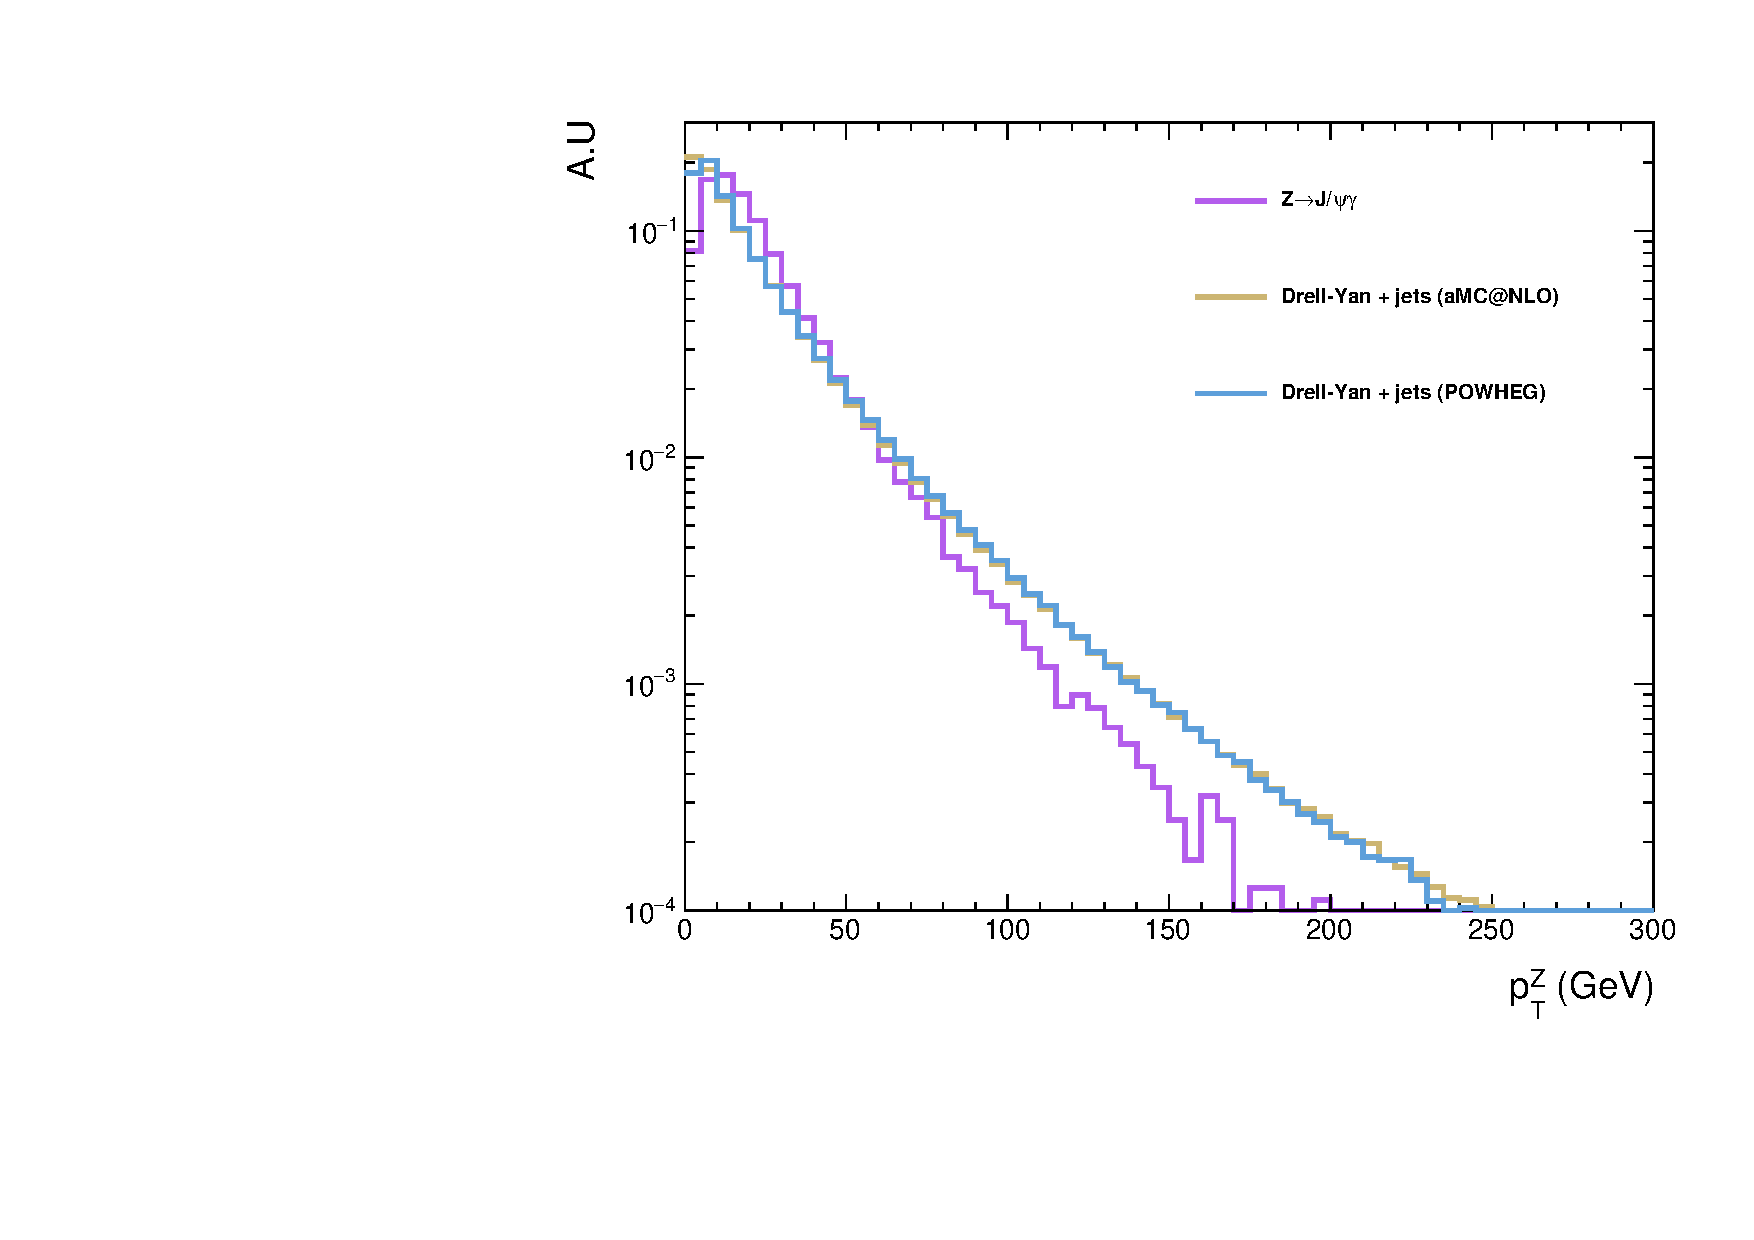
\includegraphics[width=0.5\textwidth]{Fig/ZPt_comp_withgenwei_final}~
		  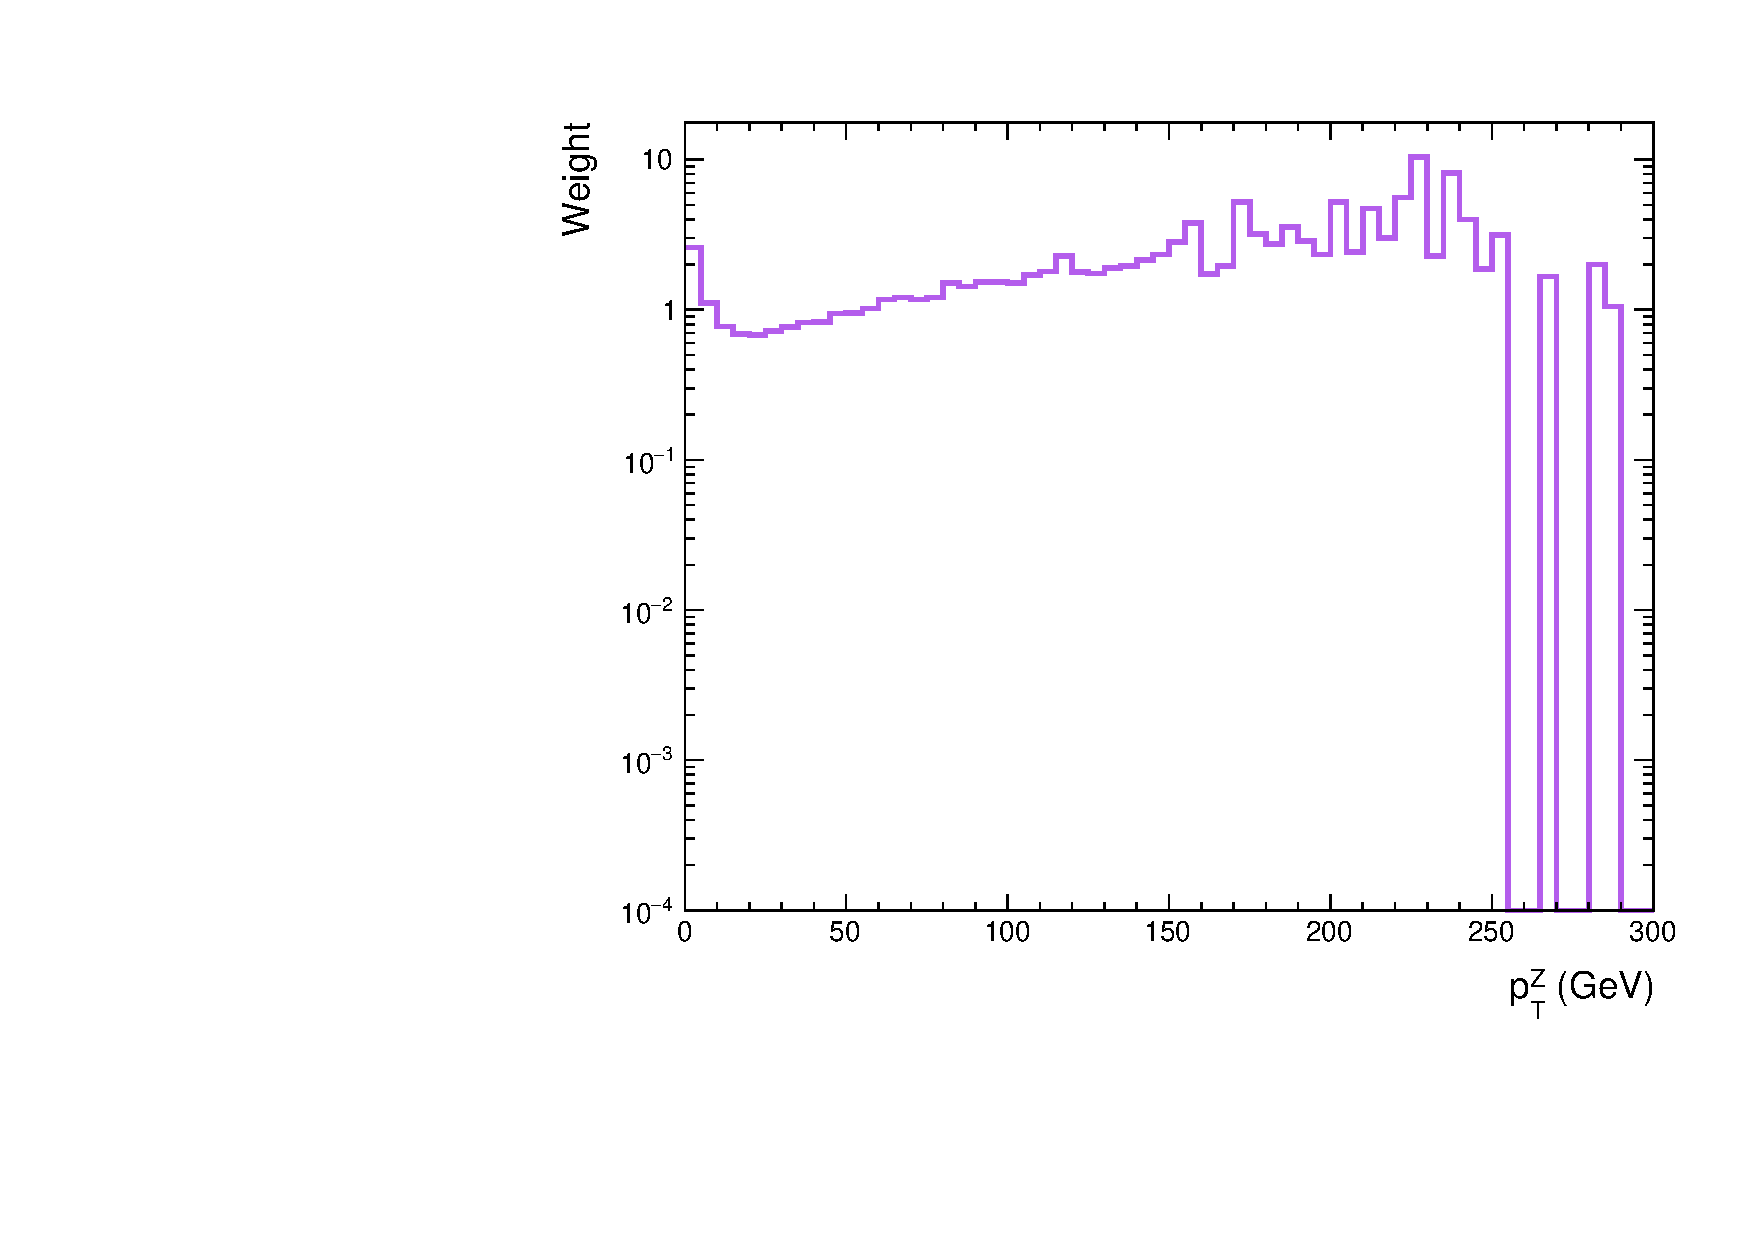
\includegraphics[width=0.5\textwidth]{Fig/ZPt_ratio_withgenwei_final}\\
		  \caption{The right plot shows the Z $\pt$ distributions at generator level of the $\cPZ\to\JPsi\ \gamma$ and Drell-Yan jets samples. The left plot shows the ratio of the two $\pt$ distributions ''Drell-Yan jets($a\MCATNLO$)'' to ''$\cPZ\to\JPsi\ \gamma$'', as binned weight to be applied to the $\PYTHIA$ sample. \label{fig:ZPtRewei}}
		  \end{center}
		\end{figure}
		
		\subsubsection*{$\JPsi$ polarization}
		The Higgs boson is now commonly believed to be a spin-0 particle, and the $\JPsi$ from its decay is therefore transversely polarized (with $\text{J}_{\text{Z}}=\pm 1$). However, this polarization is not correctly simulated in the \PYTHIA. The distribution of $cos\theta$ was checked, where $\theta$ is the angle between the muon and the direction of $\JPsi$, and is derived at the generator level. The angle $\theta$ is calculated without kinematic requirement and in the rest frame of $\JPsi$, where the direction of $\JPsi$ is obtained from the center-of-mass (CM) frame of the Higgs boson. 
		%In the Higgs Dalitz background sample, however, polarization of the $\gamma^{*}$ is correctly simulated.
		The $\PH\to\JPsi\ \gamma$ samples are therefore reweighted using weight $w = 3/4\times(1+(cos\theta)^{2})$ per event. This reweighting preserves the total number of events in the samples, however, results in a decrease of the signal acceptance by 7.0\%.
		No systematic uncertainty is assigned for this procedure since the reweighting is done via exact formula, and the angular distribution after reweighting is the one we expect. 
		Figs.~\ref{fig:JpsiPolarization} shows the distributions of the $\PH\to\JPsi\ \gamma$ samples before (green), after (blue) reweighting, and of the $\PH\to\gamma^{*}\gamma$ sample (red) where the polarization of $\gamma^{*}$ is correctly simulated.
		
		\begin{figure}[!ht]\begin{center}
		  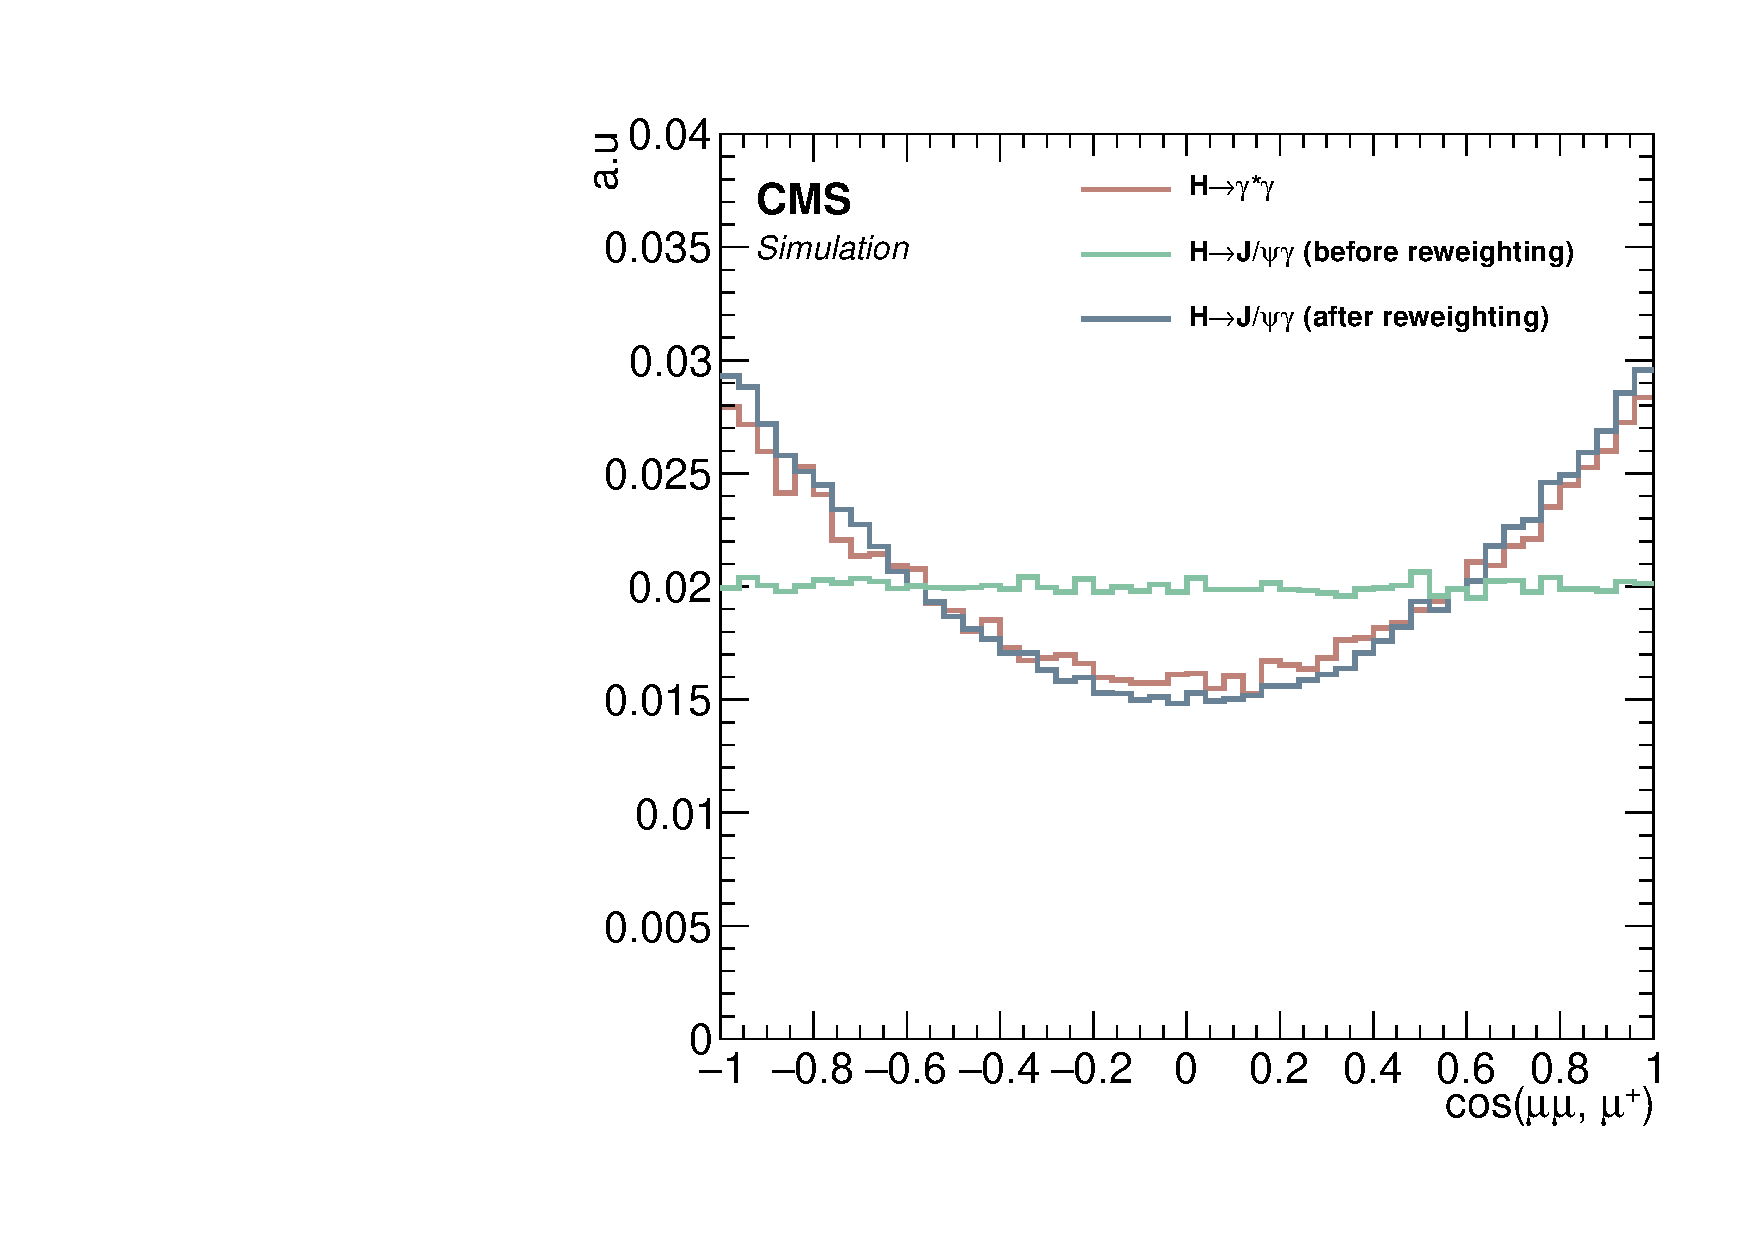
\includegraphics[width=0.7\textwidth]{Fig/GenLevel_HJpsiG/Jpsi_Polarization_H_new}
		  \caption{Distributions of $cos\theta$ of $\JPsi\to\mu\mu$ and $\gamma^{*}\to\mu\mu$. The green distribution is the $\PH\to \JPsi\ \gamma$ sample before reweighting; the red distribution is from $\PH\to \gamma^{*}\gamma$; the blue distribution is $\PH\to \JPsi\ \gamma$ sample after reweighting.}
		\label{fig:JpsiPolarization}\end{center}\end{figure} 
		
		The Z boson is a spin-1 particle, the $\JPsi$ from its decay can be transversely (with $\text{J}_{Z}=\pm 1$) or longitudinally polarized (with $\text{J}_{Z}=0$), depending on the polarization of the $\cPZ$ boson. 
		Figs.~\ref{fig:ZdecayJpsiPolarization} shows the distributions resulting from different polarization scenarios. 
		Table~\ref{tab:PolSce} summarizes the reweight formulae and effects on acceptance from different polarization scenarios.
		
		The central value of the final results is to assume the $\JPsi$ to be unpolarized. Variations resulting from the extreme scenarios (complete transverse or longitudinal) will be quoted and shown.
		
		\begin{figure}[!ht]\begin{center}
		  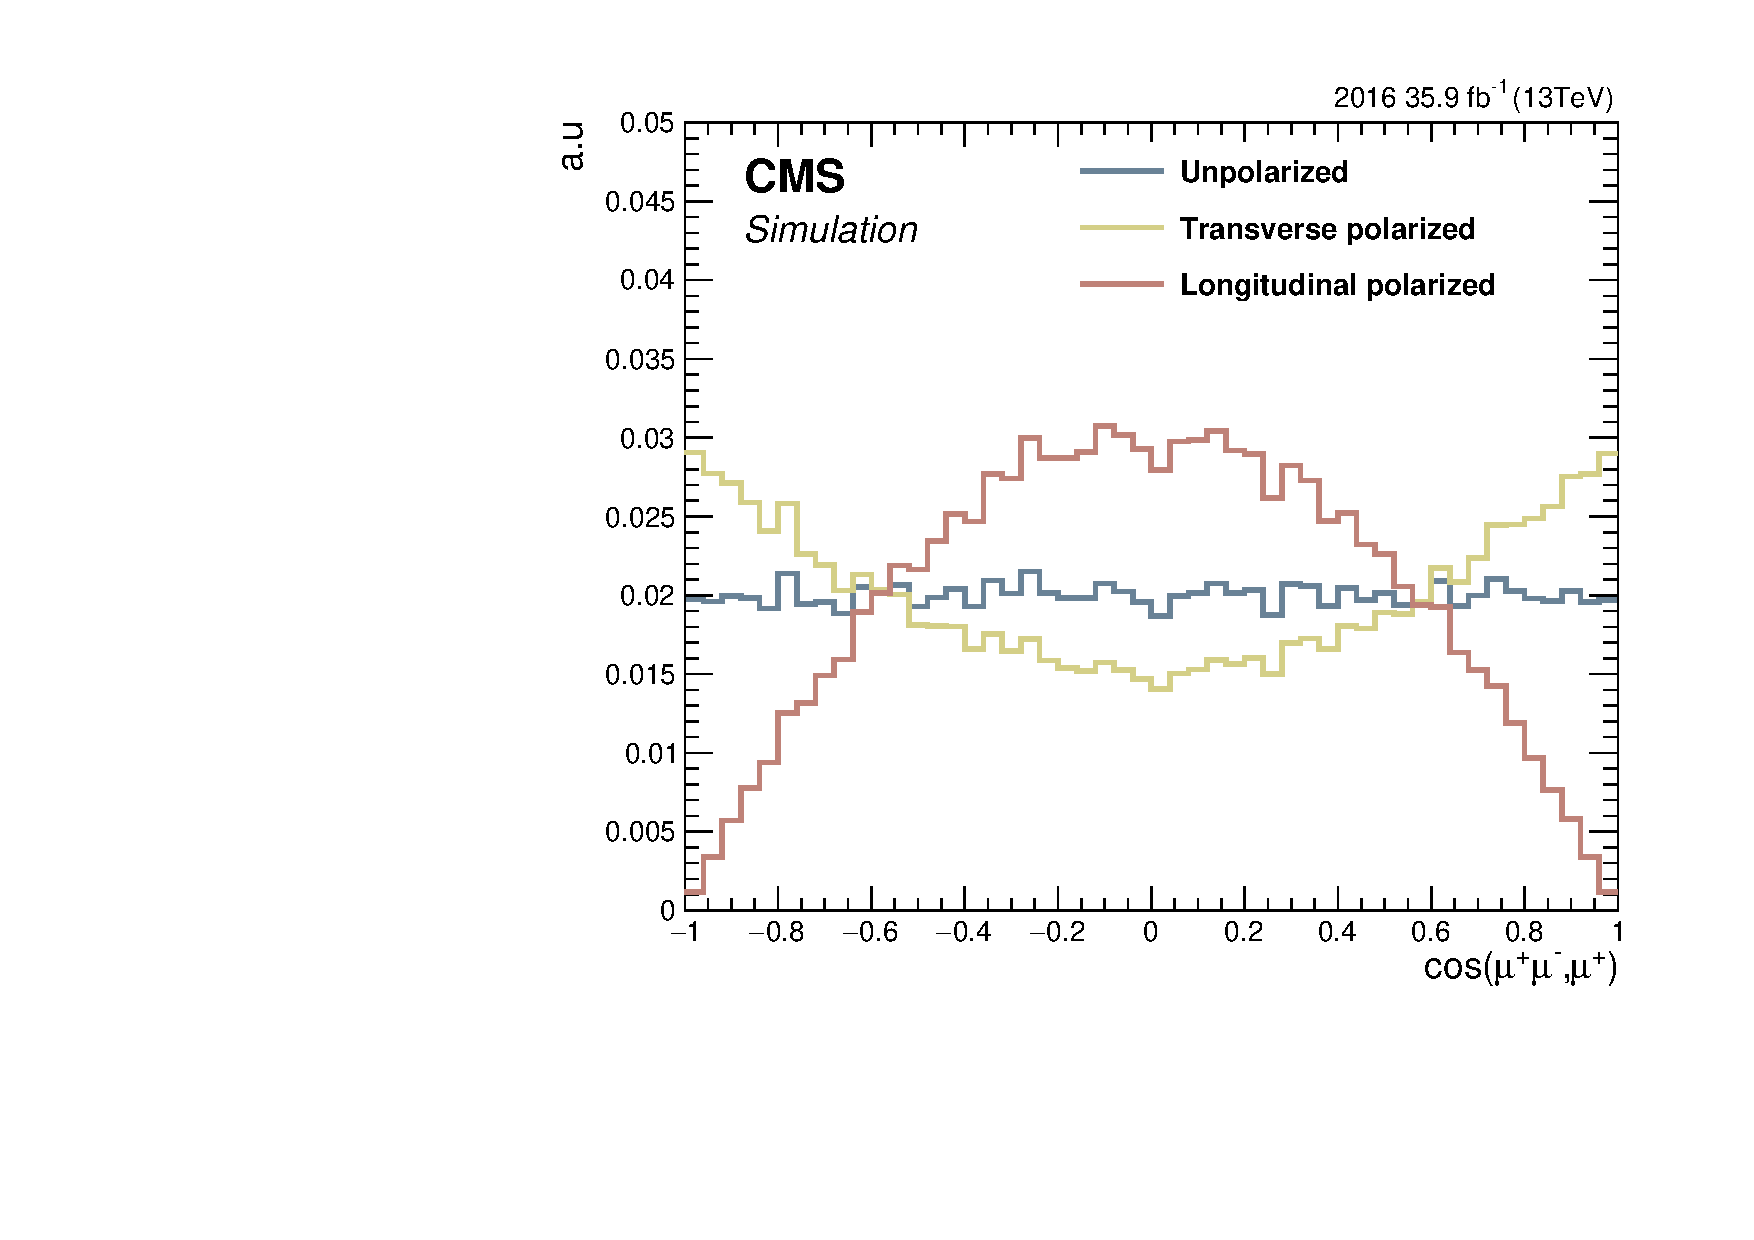
\includegraphics[width=0.7\textwidth]{Fig/GenLevel_ZJpsiG/Polarization_Scenario}
		  \caption{Distributions of $cos\theta$ of $\JPsi\to\mu\mu$ resulting from different polarization scenarios. The blue distribution is the unpolarized scenario; the earthy yellow distribution is fully transversely polarized scenario; the red distribution is fully longitudinal polarized scenario.}
		\label{fig:ZdecayJpsiPolarization}\end{center}\end{figure}
		
		\begin{table}[!ht]
		  \begin{center}
		    \begin{tabular}{|c|c|c|c|}
		    \hline
		      $\text{J}_{Z}$    & Polarization scenario   & Formula & Effect on acceptance \\ 
		      \hline
		      $\pm 1$   & Transverse   & $3/4\times(1+(cos\theta)^{2})$ & -7.8$\%$ \\
		      0   & Longitudinal   & $3/2\times(1-(cos\theta)^{2})$ & +15.6$\%$  \\
		      \hline
		    \end{tabular}
		    \caption{Summary of the reweight formulae and effects on acceptance from different polarization scenarios.\label{tab:PolSce}}
		  \end{center}
		\end{table}
		
		\subsubsection*{Background}  
The Higgs boson Dalitz decay~\cite{Abba96}, $\PH\to\gamma^{*}\gamma\to\mu\mu\gamma$, results in the same final state as the signal. This process exhibits a peak in the three-body invariant mass $m_{\mu\mu\gamma}$ at the Higgs boson mass, and is therefore referred to as a peaking, or resonant, background. It is taken into account when deriving the upper limit on the branching fraction for $\cPZ \to\JPsi\ \gamma$. The diagrams for $\PH\to\gamma^*\gamma$ process are shown in Fig.~\ref{fig:FeynmanDiagrams_Dalitz}. Samples of Higgs boson Dalitz decays, produced in ggF, VBF, V$\PH$ for $m_{\PH}=125$\GeV, are simulated at NLO using the $\MADGRAPH 5$\_a\MCATNLO 2.6.0 matrix element generator~\cite{Alwall:2014hca}, interfaced with \PYTHIA 8.212 for parton showering and hadronization. The dimuon invariant mass $m_{\mu\mu}$ in the ggF sample is restricted to be less than 50\GeV, while in VBF and V$\PH$ samples it is less than 60\GeV. The contribution of the tt$\PH$ is accounted for by scaling the VBF signal to the tt$\PH$ production cross section. The branching fraction for $\PH\to\gamma^{*}\gamma$ is obtained from MCFM 7.0.1 program~\cite{MCFM7}. The other source of peaking background comes from the decay of a Higgs boson into two muons, with a photon radiated from one of the muons. Fig.~\ref{fig:GenLevel_Hmumu} shows the distributions of some kinematic variables for the $\PH\to\PGm\PGm$ and the $\PH\to\JPsi\ \gamma$ decays. As one can see, the event signatures of the decay are different from those of the $\PH\to\JPsi\ \gamma$, the contribution of this background is found to be negligible after the event selection.		
		
\begin{table}[!ht]
		%\footnotesize
		\scriptsize
		  \begin{center}
		    \begin{tabular}{|l|l|}
		    \hline
		      Dataset name & $\mathcal{B}_{SM}(\PH\to \gamma^{*}\gamma\to\mu\mu\gamma)$                  \\ 
		      \hline
		      /GluGluHToMuMuG\_M125\_mll-0To50*/RunIISummer16*/MINIAODSIM &   3.83\ten{-5} \\
		      /VBFHToMuMuG\_M125\_MLL-0To60*/RunIISummer16*/MINIAODSIM & 3.92\ten{-5}\\
		      /ZHToMuMuG\_M125\_MLL-0To60*/RunIISummer16*/MINIAODSIM & 3.92\ten{-5}\\
		      /WHToMuMuG\_M125\_MLL-0To60*/RunIISummer16*/MINIAODSIM & 3.92\ten{-5}\\
		      \hline
		    \end{tabular}
		    \caption{Summary of Higgs Dalitz decay samples.\label{tab:HiggsDalitzSample}}
		  \end{center}
		\end{table}		
		
\begin{figure}[!ht]
  \begin{center}  
    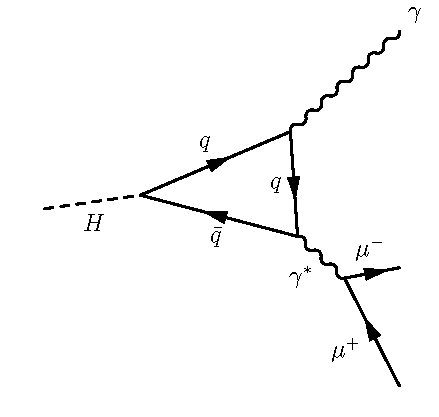
\includegraphics[width=0.33\textwidth]{Fig/HDalitz_1}~
    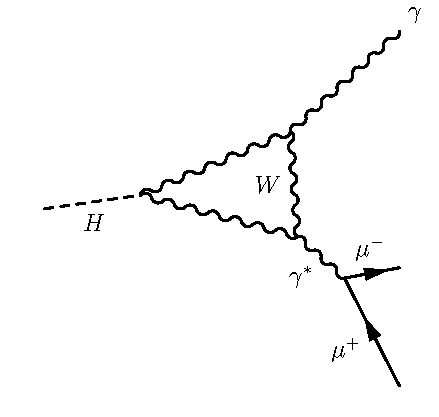
\includegraphics[width=0.33\textwidth]{Fig/HDalitz_2}~
    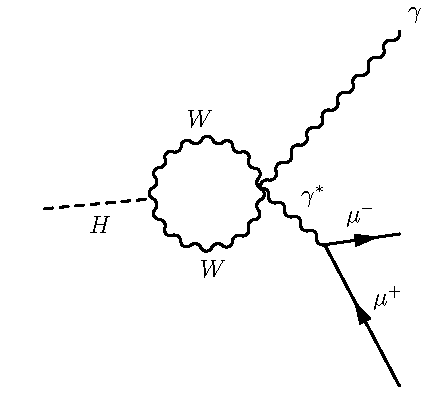
\includegraphics[width=0.33\textwidth]{Fig/HDalitz_3}\\
    \caption{Main diagrams for the Higgs Dalitz decay, $\PH\to\gamma^{*}\gamma\to\mu\mu\gamma$. \label{fig:FeynmanDiagrams_Dalitz}}  
  \end{center}
\end{figure} 

\begin{figure}[p]
  \begin{center}  
    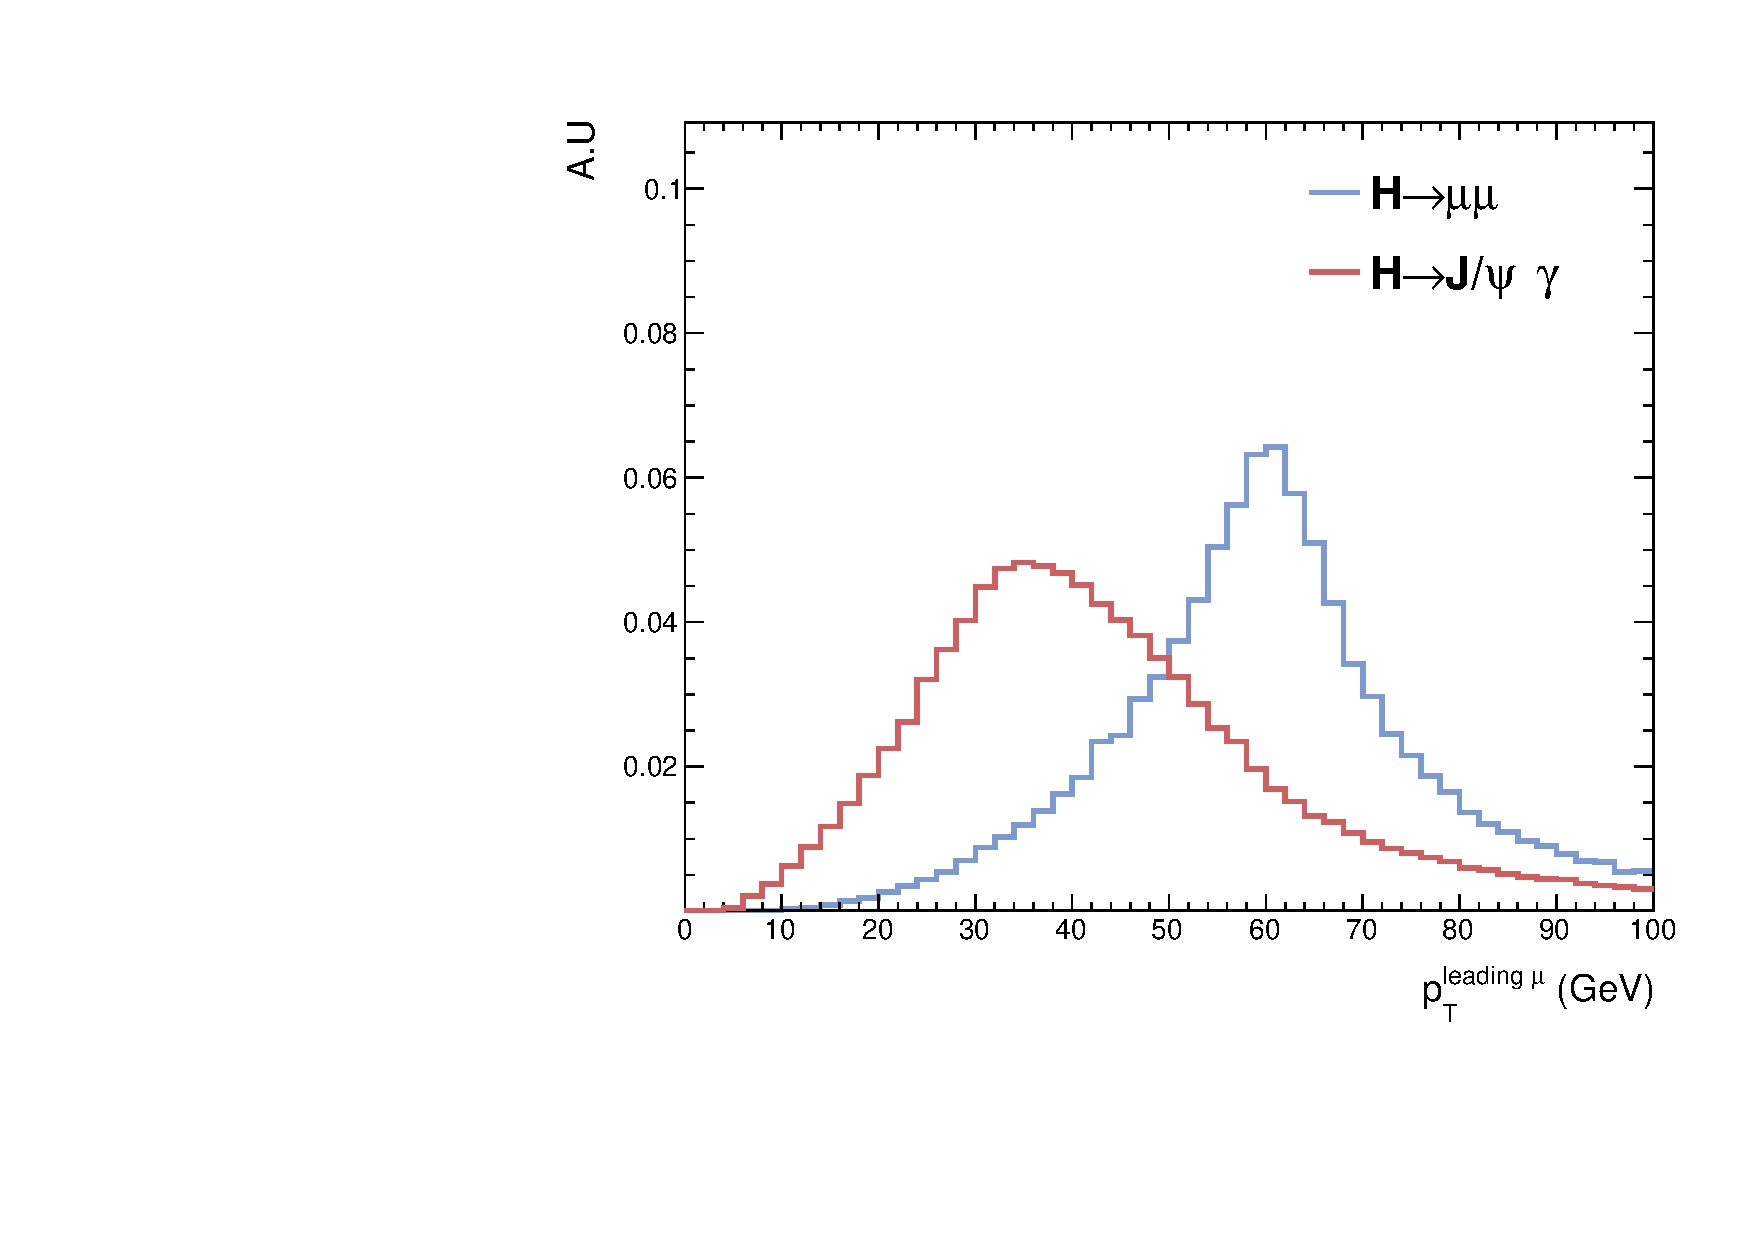
\includegraphics[width=0.5\textwidth]{Fig/GenLevel_Hmumu/Hmumu_mu1Pt}~
    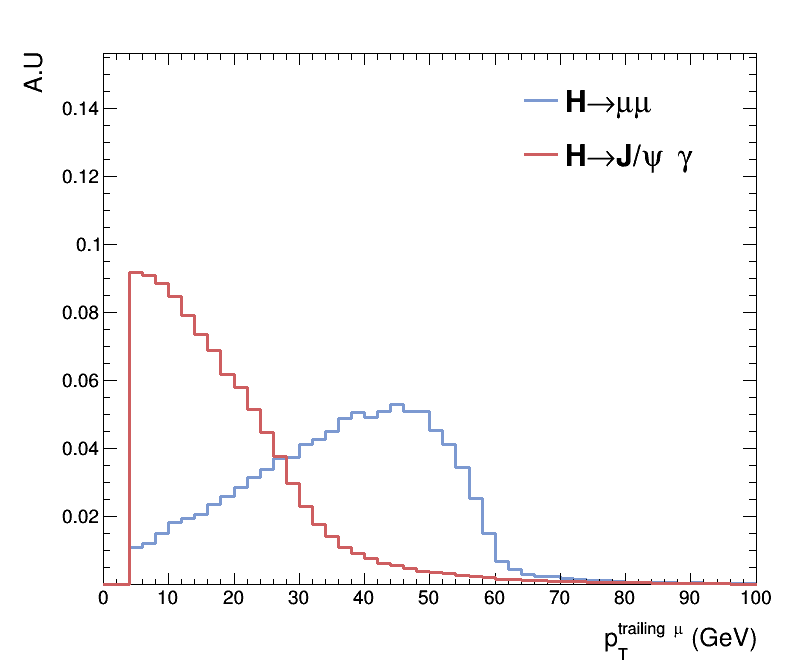
\includegraphics[width=0.5\textwidth]{Fig/GenLevel_Hmumu/Hmumu_mu2Pt}\\
    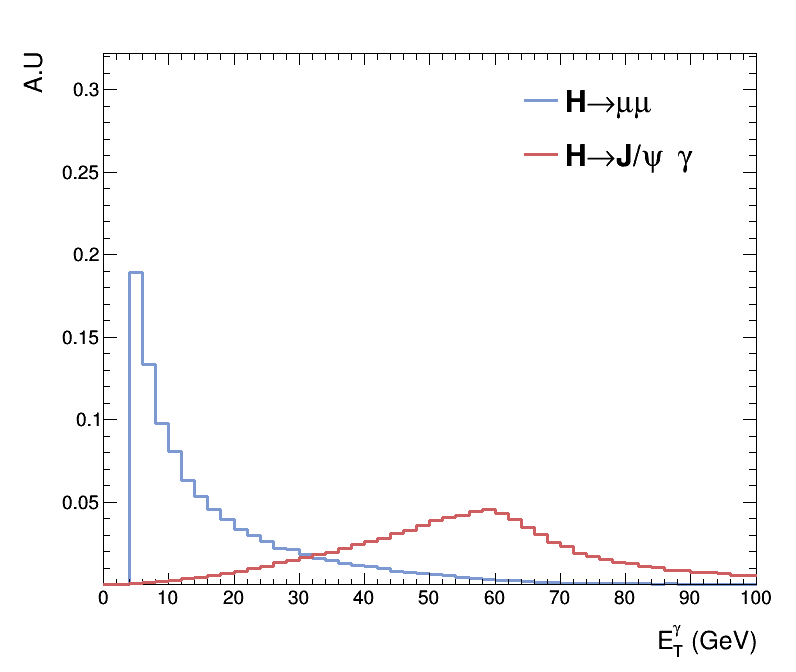
\includegraphics[width=0.5\textwidth]{Fig/GenLevel_Hmumu/Hmumu_phoEt}~
    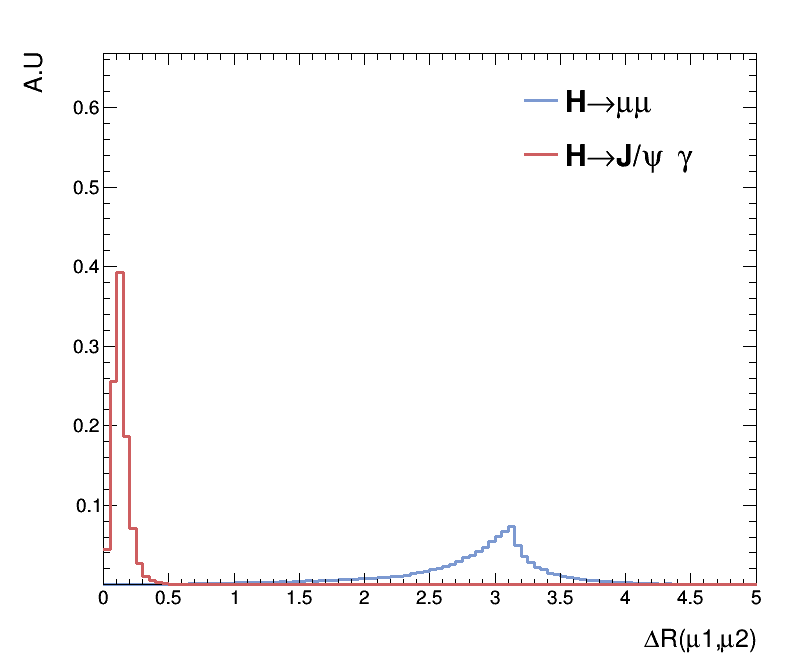
\includegraphics[width=0.5\textwidth]{Fig/GenLevel_Hmumu/Hmumu_dRdimuon}\\
    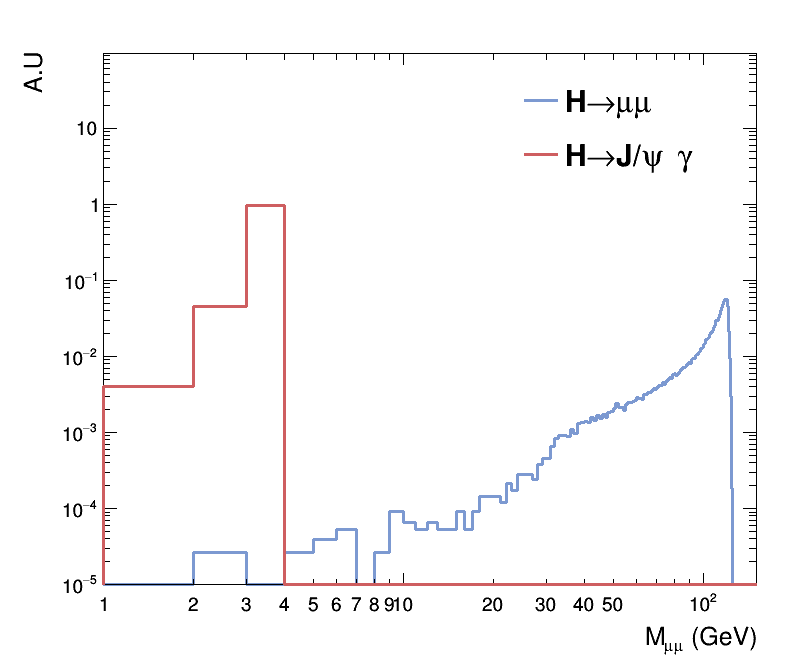
\includegraphics[width=0.5\textwidth]{Fig/GenLevel_Hmumu/Hmumu_Mmumu}~
    \caption{Distributions of kinematic variables for the $\PH\to\PGm\PGm$ and the $\PH\to\JPsi\ \gamma$ decays. (Top left) $\pt$ of the leading muon; (Top middle) $\pt$ of the treailing muon; (Top right) $\et$ of the photon; (Bottom left) angular separation $\Delta \text{R}$ between muons; (Bottom right) dimuon mass $m_{\PGm\PGm}$.  \label{fig:GenLevel_Hmumu}}  
  \end{center}
\end{figure} 

Similarly, the Drell--Yan process, $\Pp\Pp\to\cPZ\to\mu\mu\gamma$ is a peaking background for $\cPZ \to\JPsi\ \gamma$. 
The diagrams for the $\Pp\Pp\to\cPZ\to\mu\mu\gamma$ process are shown in Fig.~\ref{fig:FeynmanDiagrams_Zmmg}.
The $\MADGRAPH 5$\_a\MCATNLO 2.6.0 generator at leading order with the NNPDF3.0 PDF set, interfaced with \PYTHIA 8.226 for parton showering and hadronization with tune CUETP8M1, is used to generate a sample of these resonant background events. The photons in these events are all produced in final-state radiation from the $\Z\to\mu\mu$ decay and therefore the $m_{\mu\mu\gamma}$ distribution peaks at the $\cPZ$ boson mass and there is no continuum contribution. Kinematic requirements, such as $2<m_{\mu\mu}<15\GeV$ and $\et^{\gamma}>20\GeV$, are imposed when generating the sample, and results in an inclusive cross section of 93.0 pb.
\begin{figure}[!ht]
  \begin{center}  
    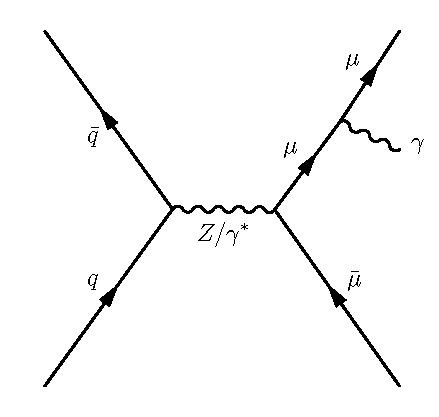
\includegraphics[width=0.35\textwidth]{Fig/Zmmg1}~
    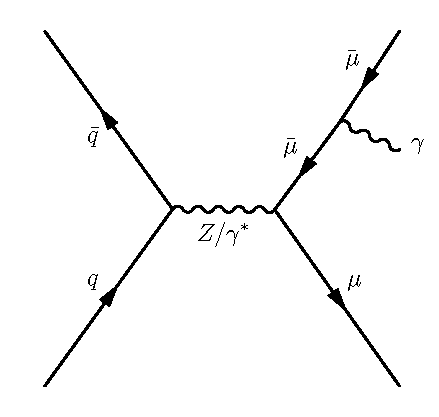
\includegraphics[width=0.35\textwidth]{Fig/Zmmg2}
    \caption{Main diagrams for the Drell-Yan process, $\Pp\Pp\to\cPZ\to\mu\mu\gamma$.\label{fig:FeynmanDiagrams_Zmmg}}  
  \end{center}
\end{figure}
The additional photons added by \PYTHIA may modify the photon $\et$ modeling in the sample. The effect is checked by using generator level information.
		Figs.~\ref{fig:ZGPYTHIA} shows two distributions, one is the $\et$ of the photons which are prompt final states\footnotemark (in blue) and the other one is the $\et$ of the photons added by the $\PYTHIA8$ when it is interfaced with $a\MCATNLO$ (in red). The number of photons with $\et > 33 \GeV$ added by $\PYTHIA8$ is only 0.3\% of those from hard scattering. Therefore, the interface with $\PYTHIA$ has minimal effect on the overall photon $\et$ spectrum, and no additional uncertainty is assigned.
		\footnotetext{A particle is labeled as prompt if it is from the hard process in an interaction.}
		\begin{figure}[!ht]
		\begin{center}
		  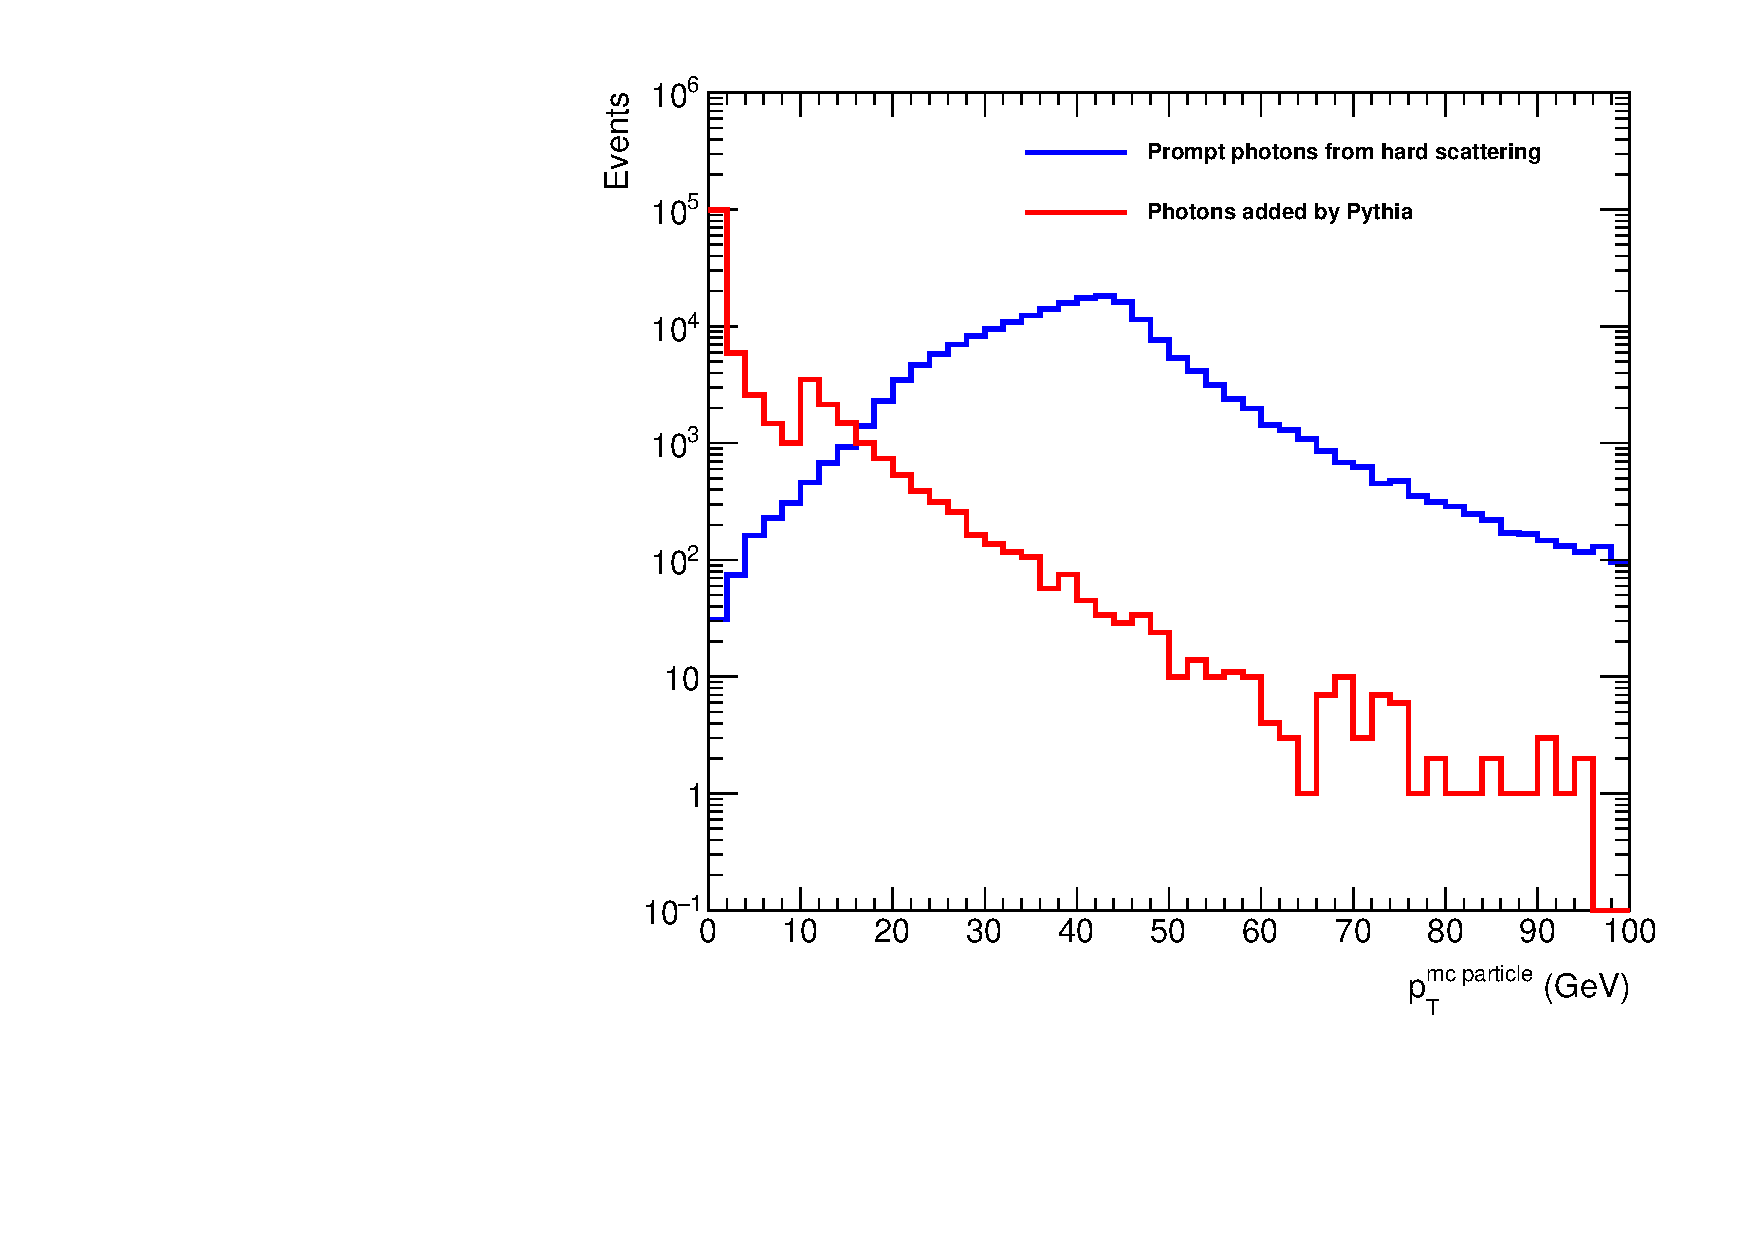
\includegraphics[width=0.7\textwidth]{Fig/mcPt_FromMEPythia}
		  \caption{The $\et$ of the photons which are prompt final state (in blue) and the other one is the $\et$ of the photons added by the $\PYTHIA$ when it is interfaced with $a\MCATNLO$ (in red).}
		\label{fig:ZGPYTHIA}
		\end{center}
		\end{figure}

There are also background processes that do not give resonance peaks in the three-body invariant mass spectrum. These are referred to as non-peaking (non-resonant) backgrounds. 
These processes include 
%inclusive quarkonium production associated with jets or photon where energetic jets can be misidentified as photon ($\Pp\Pp\to \JPsi+\text{jets}/\gamma$), the Drell-Yan process with associated jets ($\Pp\Pp\to\cPZ/\gamma^{*}+\text{jets}$), and associated photon plus jets production ($\Pp\Pp\to\gamma+\text{jets}$). 
		\begin{itemize}
		\item The Drell-Yan FSR process: $\Pp\Pp\rightarrow \cPZ+\gamma_{\text{FSR}}\rightarrow\mu\mu\gamma_{\text{FSR}}$, where $\text{m}_{\mu\mu\gamma}$ is within the Higgs (Z) mass window.
		\item The Drell-Yan ISR process: $\Pp\Pp\rightarrow \cPZ/\gamma^{*}+\gamma_{\text{ISR}}\rightarrow\mu\mu\gamma_{\text{ISR}}$, where $\text{m}_{\mu\mu}$ is within the $\JPsi$ mass window and $\text{m}_{\mu\mu\gamma}$ is within the Higgs (Z) mass window. 
		\item $\Pp\Pp\rightarrow \cPZ/\gamma^* (\rightarrow\mu\mu)$ + jets, where a jet is misidentified as an energetic photon which can fire the trigger and pass the event requirements.
		\item $\Pp\Pp\rightarrow\gamma$ + jets, where the muons can come from the jets.
		\item Inclusive quarkonium production with a jet reconstructed as a photon $\Pp\Pp\to \JPsi+\text{jets}/\gamma$, where the muons come from the quarkonium, $\JPsi$, in our cases.
		\end{itemize}
		Since currently no proper simulated samples for those processes are available, these non-resonant backgrounds are modeled using the fits to $m_{\mu\mu\gamma}$ in data, which will be introduced in Sec.~\ref{sec:BkgModel}.
		
		\subsubsection*{Pile-up reweighting}
		The simulated sample is reweighted in analysis level using minimum bias events with cross section of $69.2\text{mb}$. The corresponding systematic uncertainties are described in Sec.~\ref{sec:Systematic}, and are estimated to be less than 1.5\% on the expected yields of the signal for both the Higgs and Z boson decays.
		
		\section{Trigger}  
		The HLT\_Mu17\_Photon30\_CaloIdL\_L1ISO trigger is used in this analysis. 
		%This dedicated trigger was originally developed and designed in Run1 analysis. 
		At the L1 (L1\_Mu5IsoEG18), the trigger requires the presence of a muon with \pt greater than 5\GeV and an isolated electromagnetic object with \pt greater than 18\GeV . The main HLT requires a muon and a photon with \pt greater than 17\GeV and 30\GeV, respectively.  
		No isolation requirement is imposed on the muon by the fact that the small angular separation between muons in the final state. 
		\subsection*{The choice of the trigger}
		A study is made to compare the resulting signal efficiency with different triggers.
		In the single muon trigger, the \pt threshold on muon is high and there is isolation requirement calculated in the cone $\Delta R=0.3$. For the double muon trigger, the $\pt$ cut of 8\GeV is imposed on the subleading muon, and there are requirements on the isolation calculated using tracker information. 
		Among the triggers used in analyses associated with heavy flavor or quarkonium physics, most of them are pre-scaled and target at different physics content. The only suitable choice is the HLT\_Dimuon20\_Jpsi\_v6. The L1 seed of this quarkonium trigger requires two muons of $\pt$ greater than 13 and 6\GeV respectively.  
		
		\begin{table}[!ht]
		\begin{center}
		\begin{tabular}{| l |} 
		\hline
		Trigger path \\ 
		\hline
		Single muon trigger \\
		~~~~HLT\_IsoMu24\_v* OR \\
		~~~~HLT\_IsoTkMu24\_v* \\
		Double muon trigger \\
		~~~~HLT\_Mu17\_TrkIsoVVL\_Mu8\_TrkIsoVVL\_v* OR \\
		~~~~HLT\_Mu17\_TrkIsoVVL\_TkMu8\_TrkIsoVVL\_v* OR \\
		~~~~HLT\_Mu17\_TrkIsoVVL\_Mu8\_TrkIsoVVL\_DZ\_v* OR \\
		~~~~HLT\_Mu17\_TrkIsoVVL\_TkMu8\_TrkIsoVVL\_DZ\_v \\
		Muon-Photon trigger \\
		~~~~HLT\_Mu17\_Photon30\_CaloIdL\_L1ISO\_v* \\
		Quarkonium trigger \\
		~~~~HLT\_Dimuon20\_Jpsi\_v* \\
		\hline
		\end{tabular}
		\caption{Triggers used in the signal efficiency study. \label{table:vartrigs}}
		\end{center}                                                                                                                                       
		\end{table} 
		
		\begin{figure}[p]
		  \centering
		    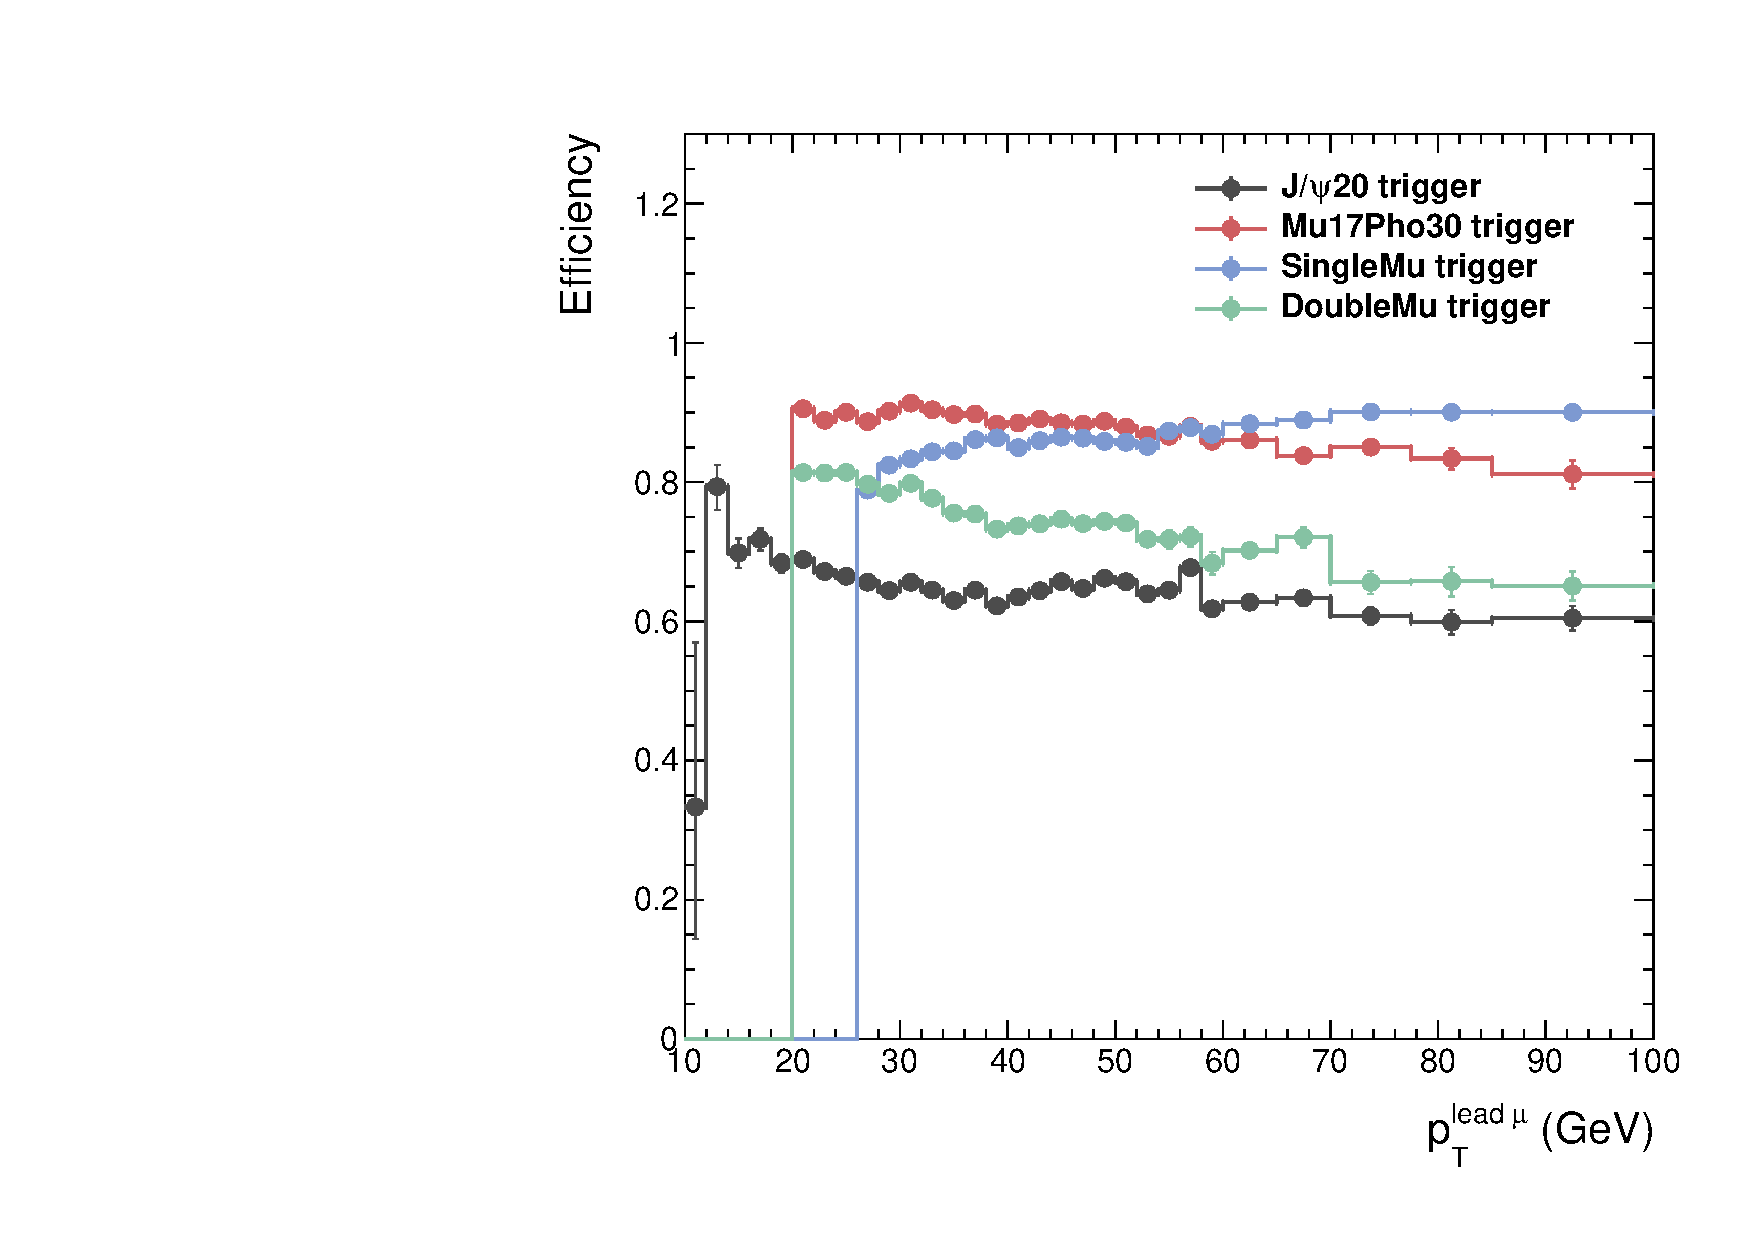
\includegraphics[width=0.45\textwidth]{Fig/Trigger/Eff_Mu1Pt_HJpsiG_Comp}~
		    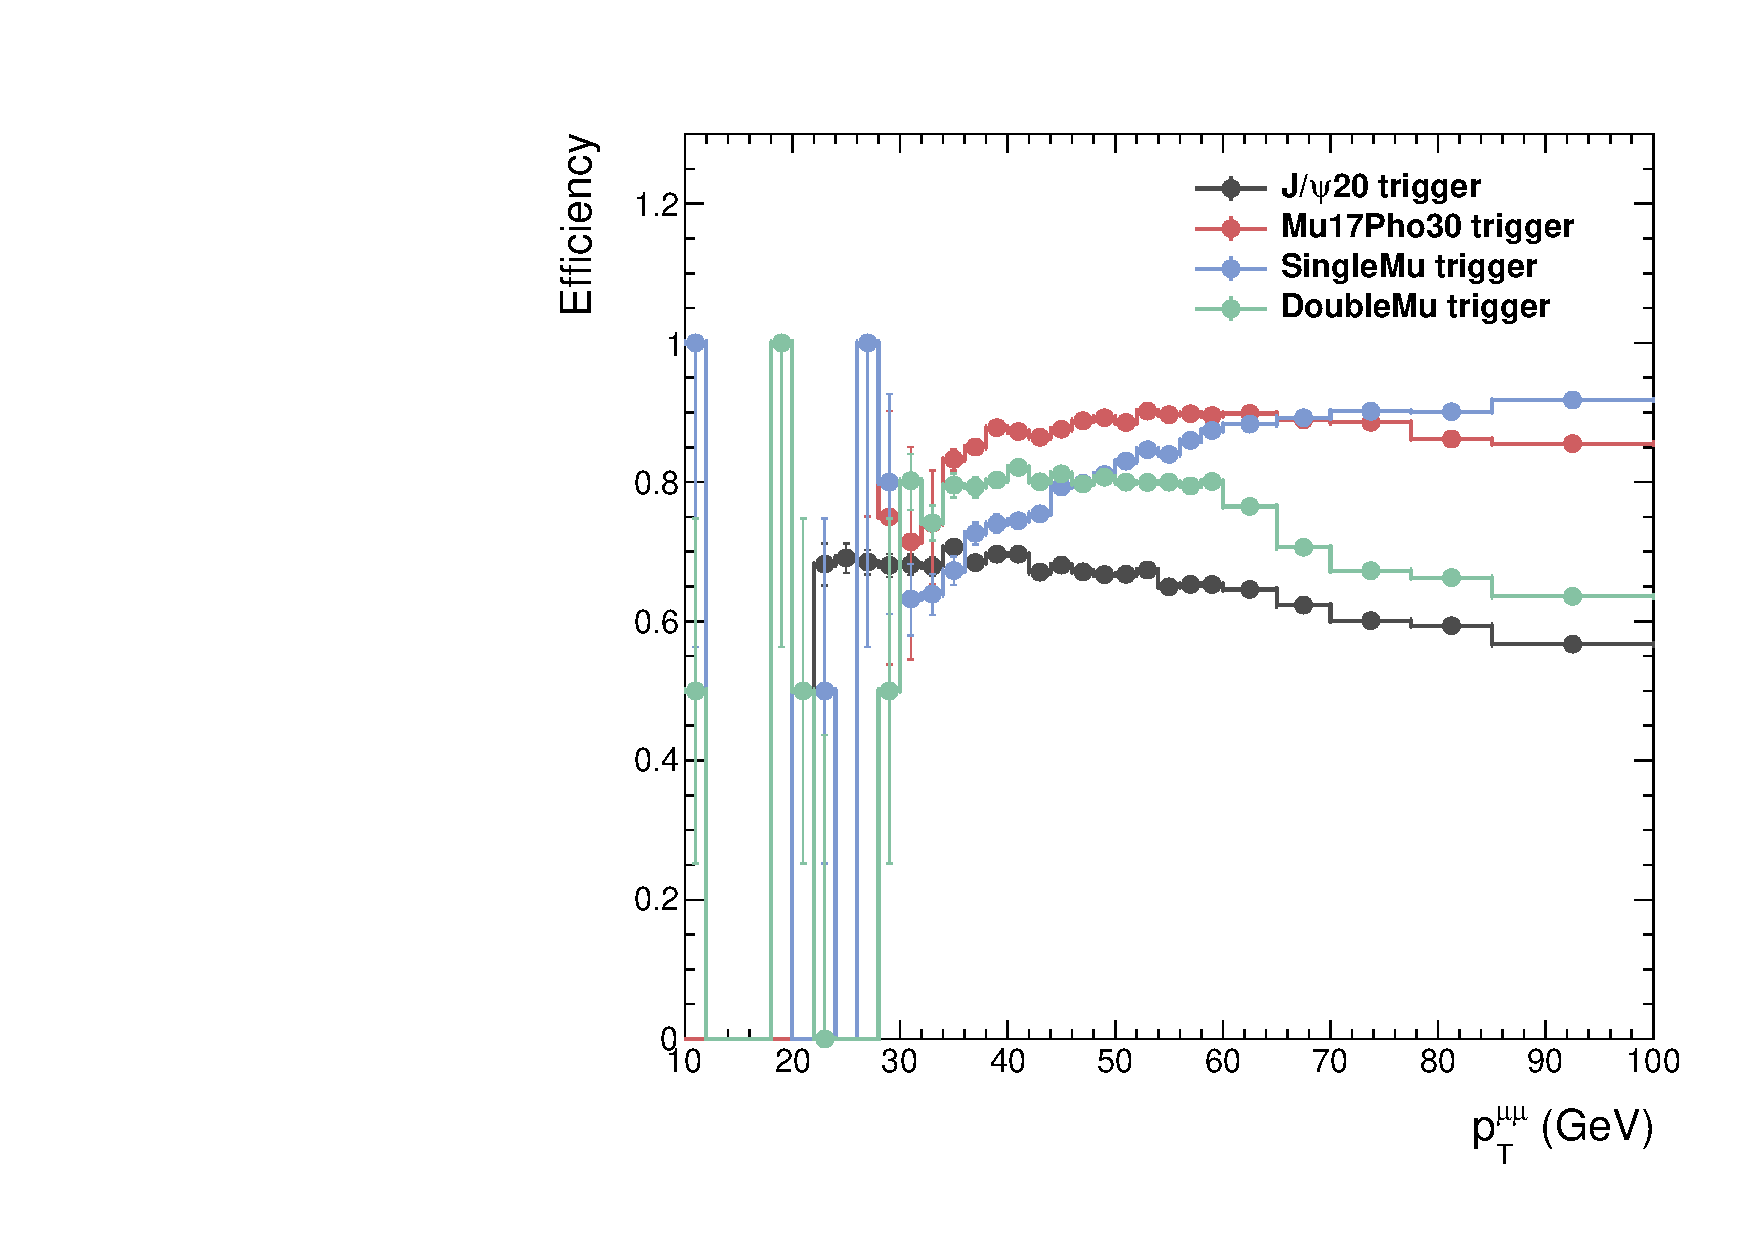
\includegraphics[width=0.45\textwidth]{Fig/Trigger/Eff_ptmumu_HJpsiG_Comp}\\
		    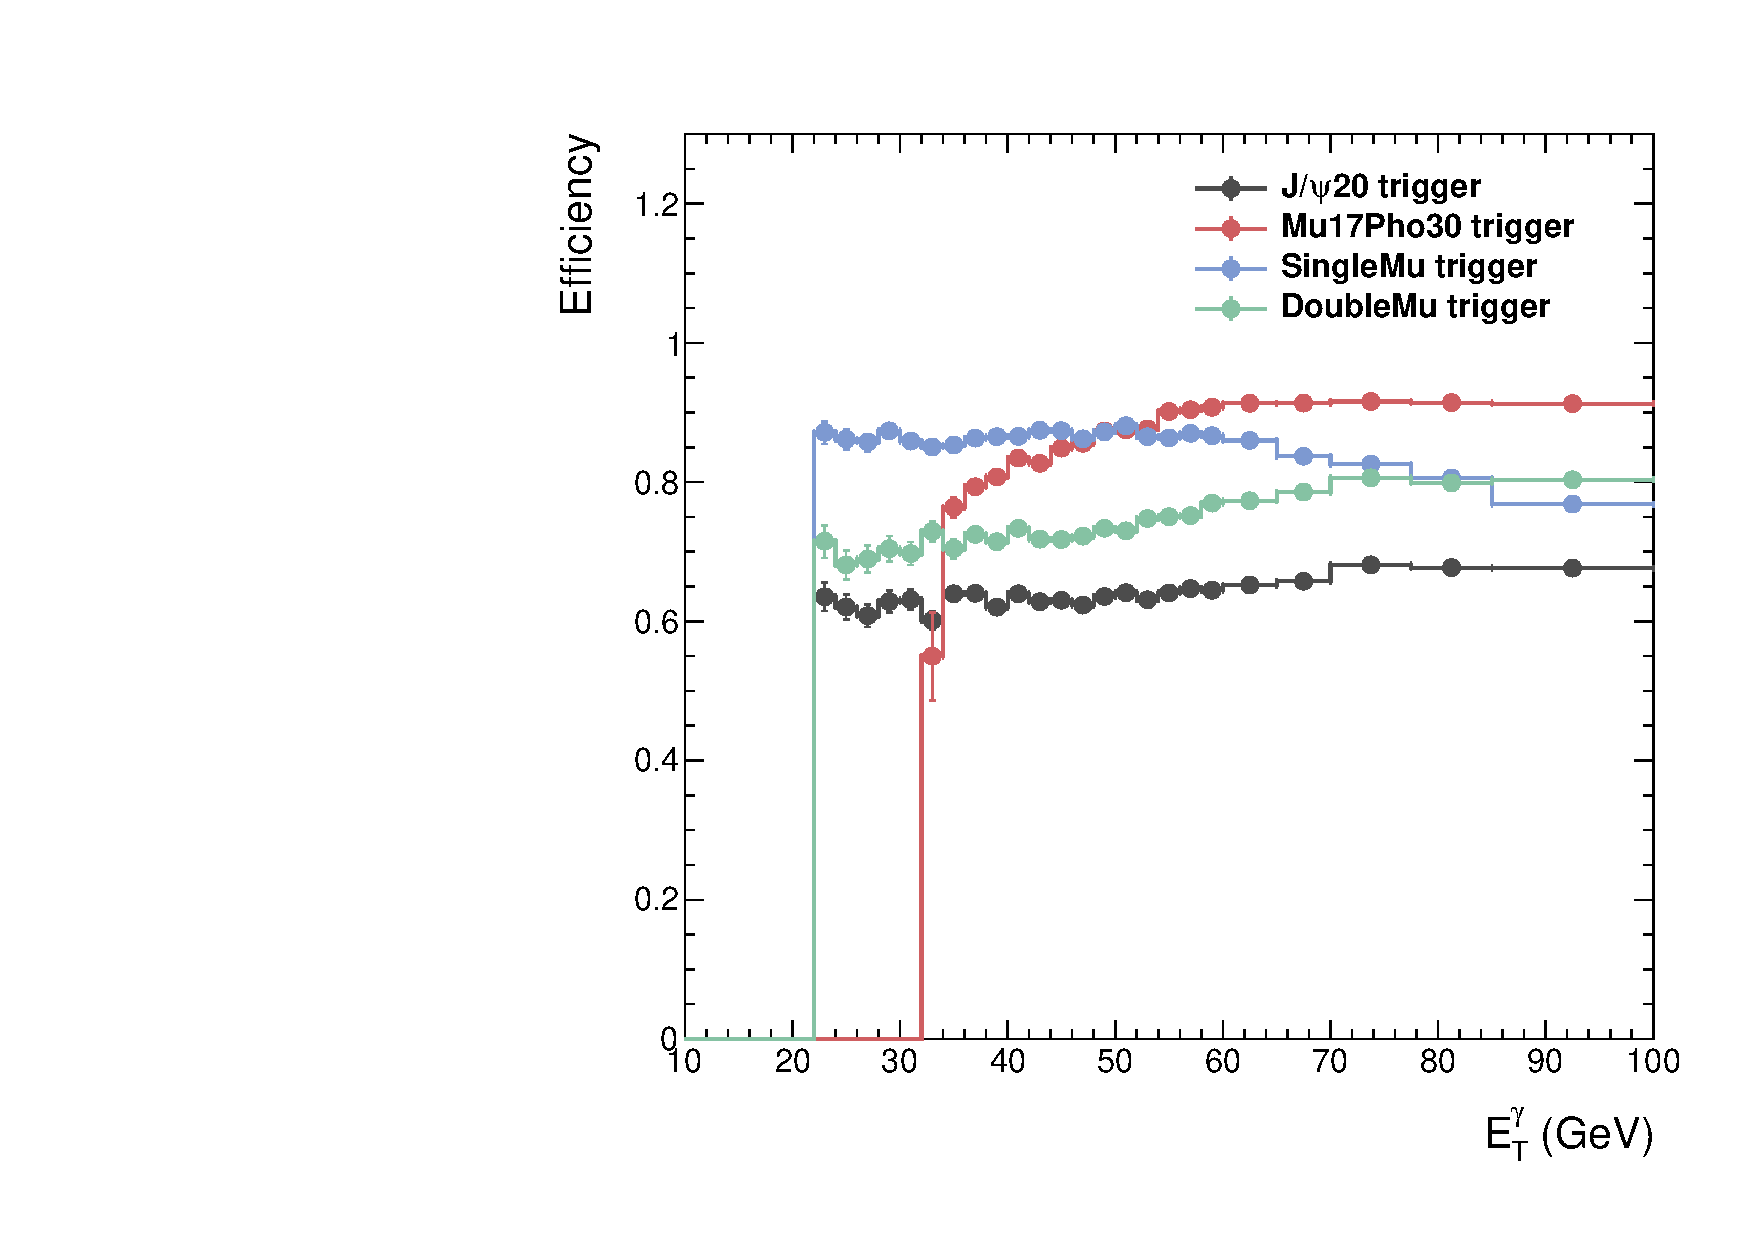
\includegraphics[width=0.45\textwidth]{Fig/Trigger/Eff_EtPho_HJpsiG_Comp}~
		    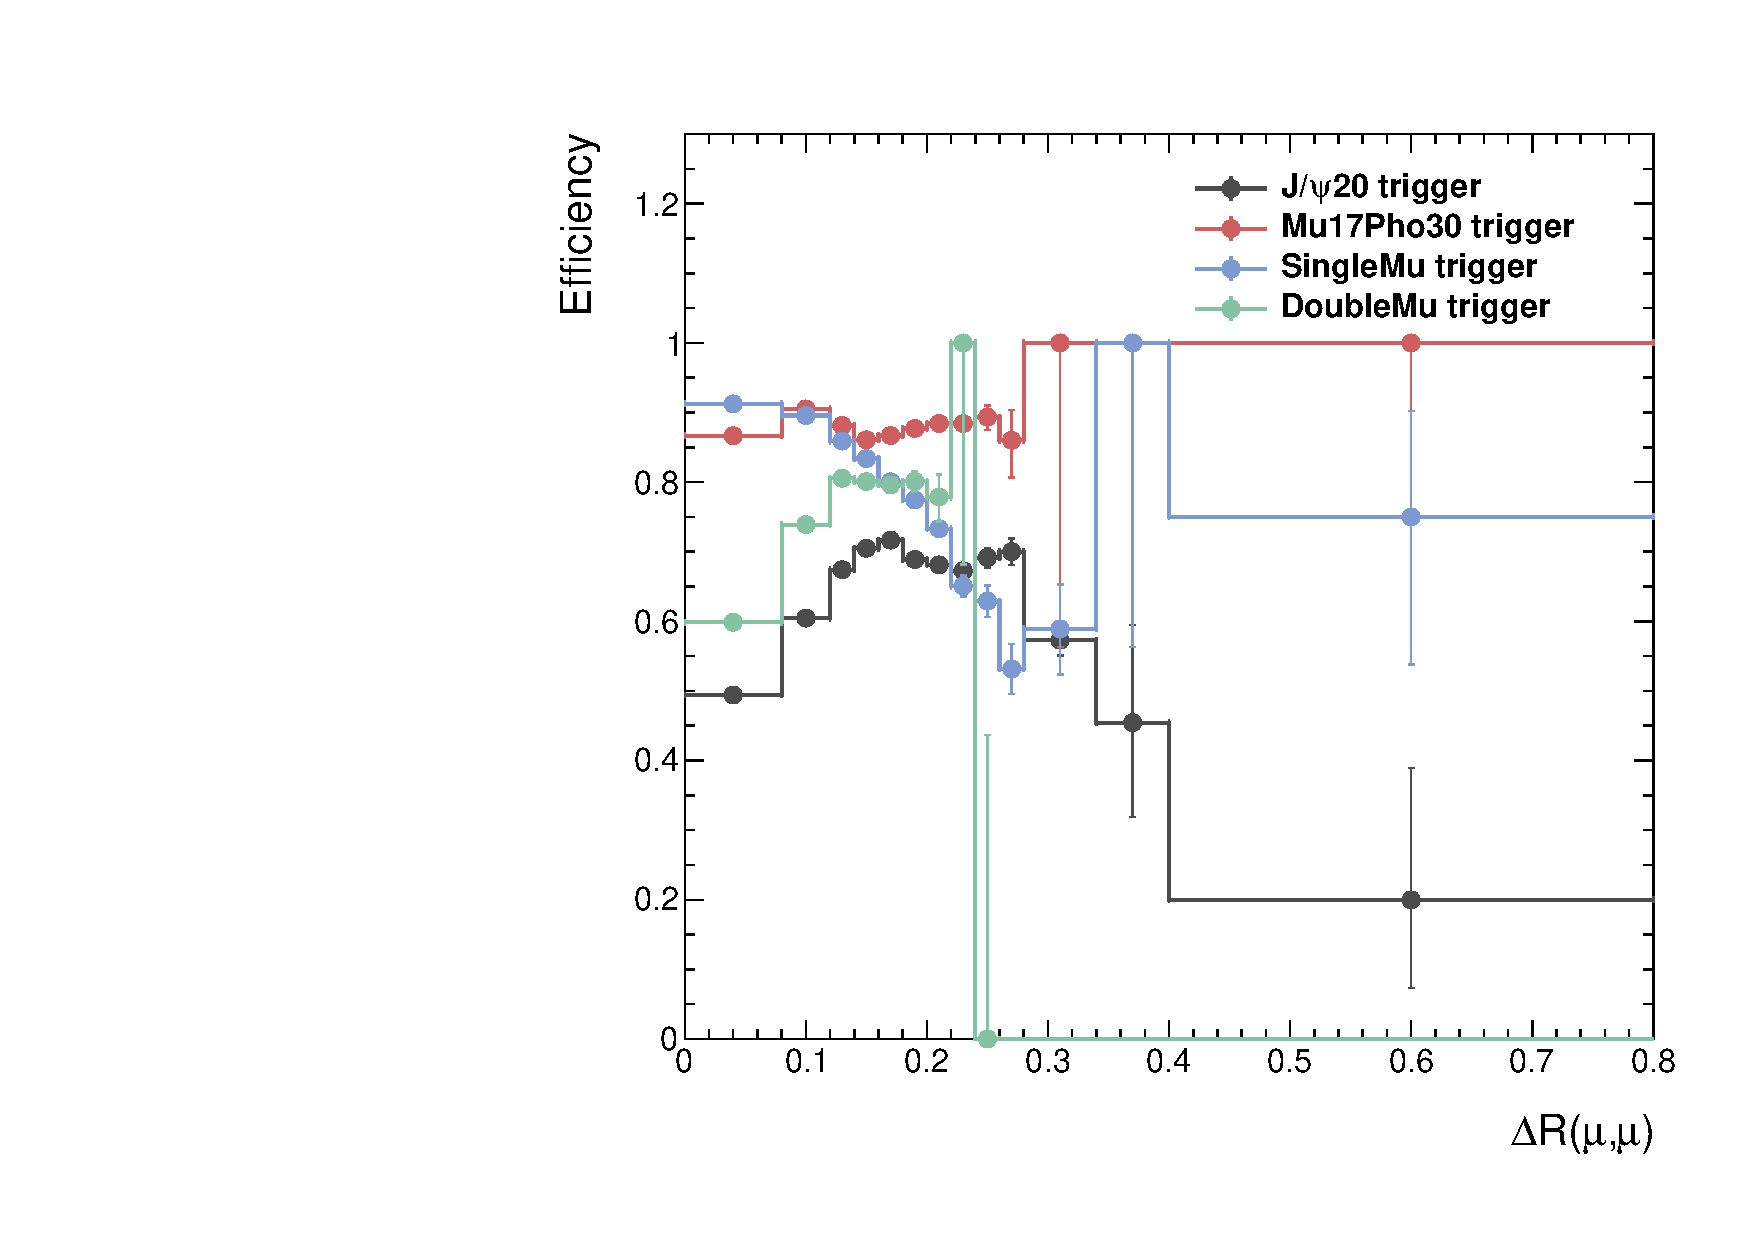
\includegraphics[width=0.45\textwidth]{Fig/Trigger/Eff_dR_HJpsiG_Comp}\\
		    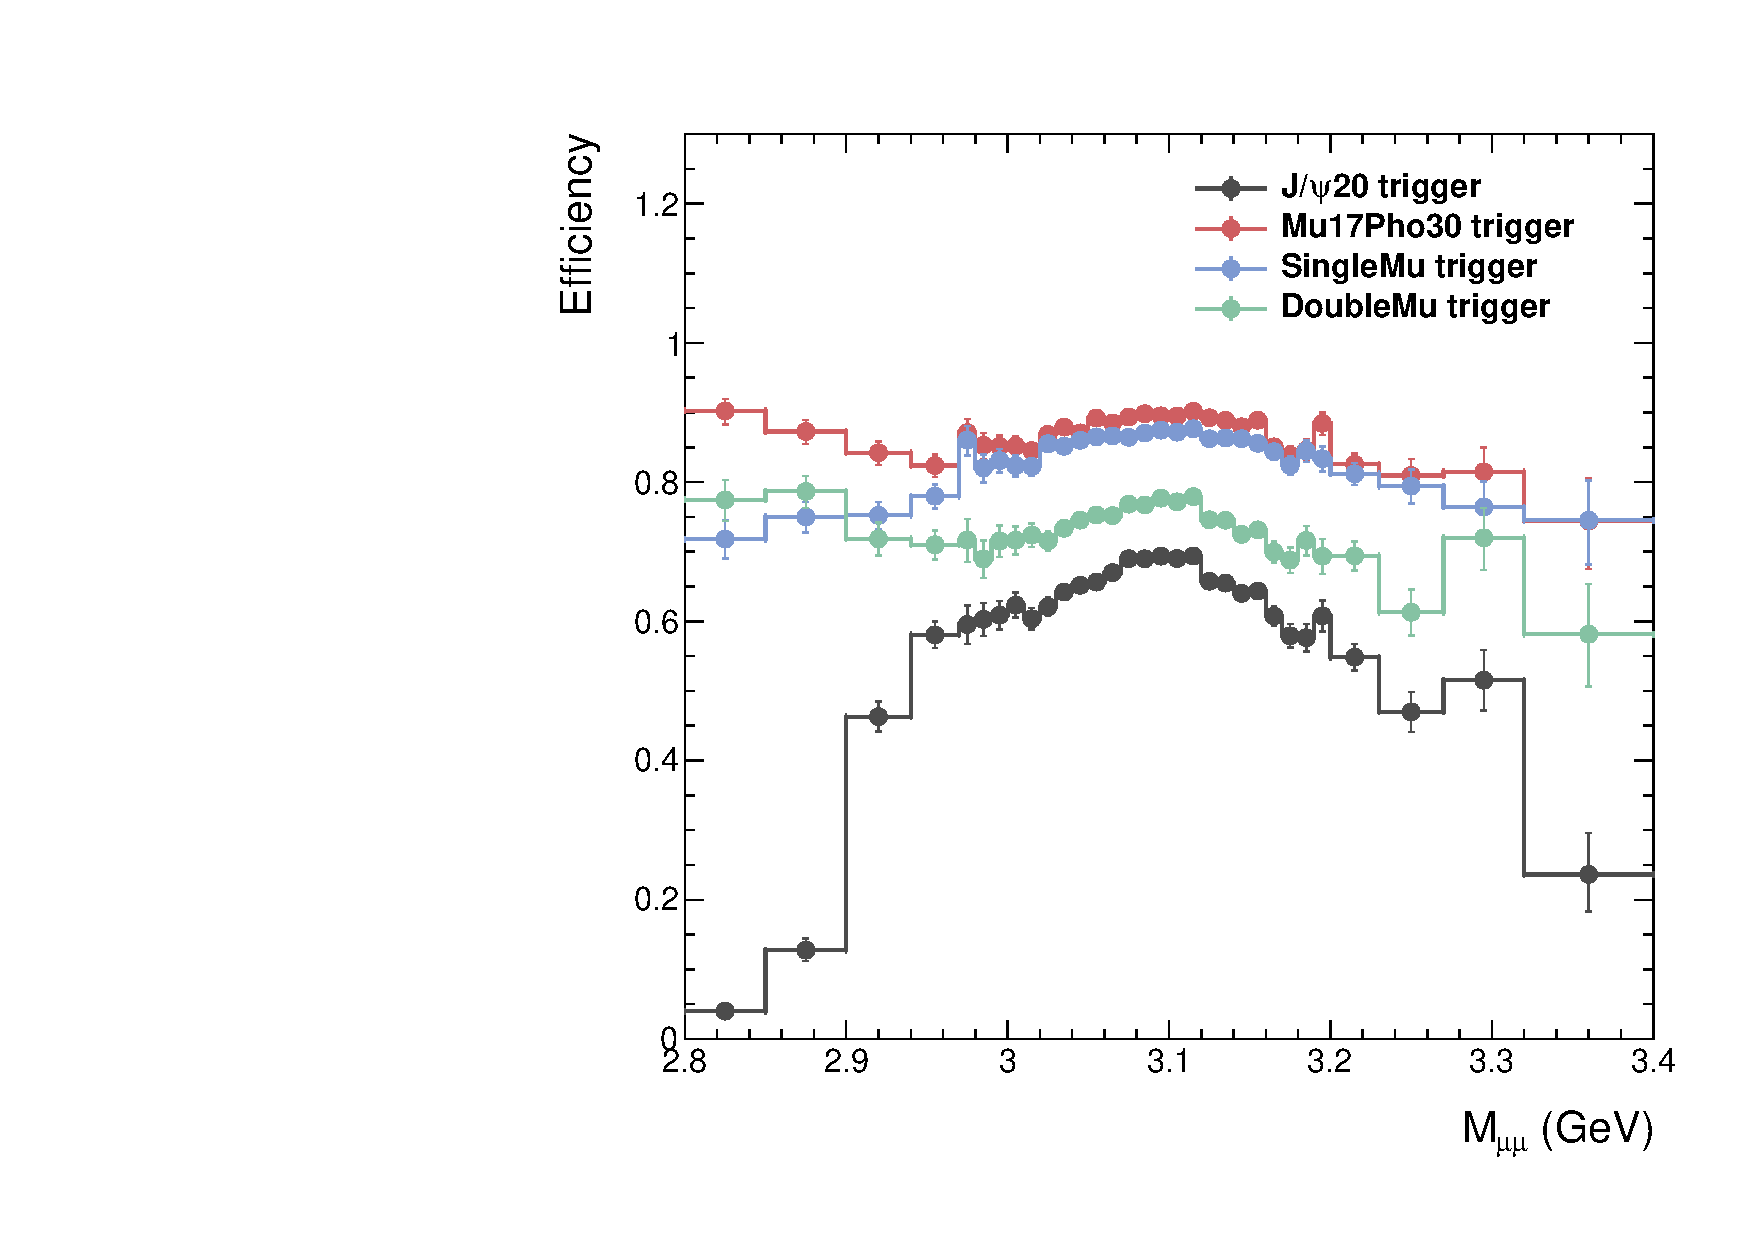
\includegraphics[width=0.45\textwidth]{Fig/Trigger/Eff_Mmumu_HJpsiG_Comp}~
		    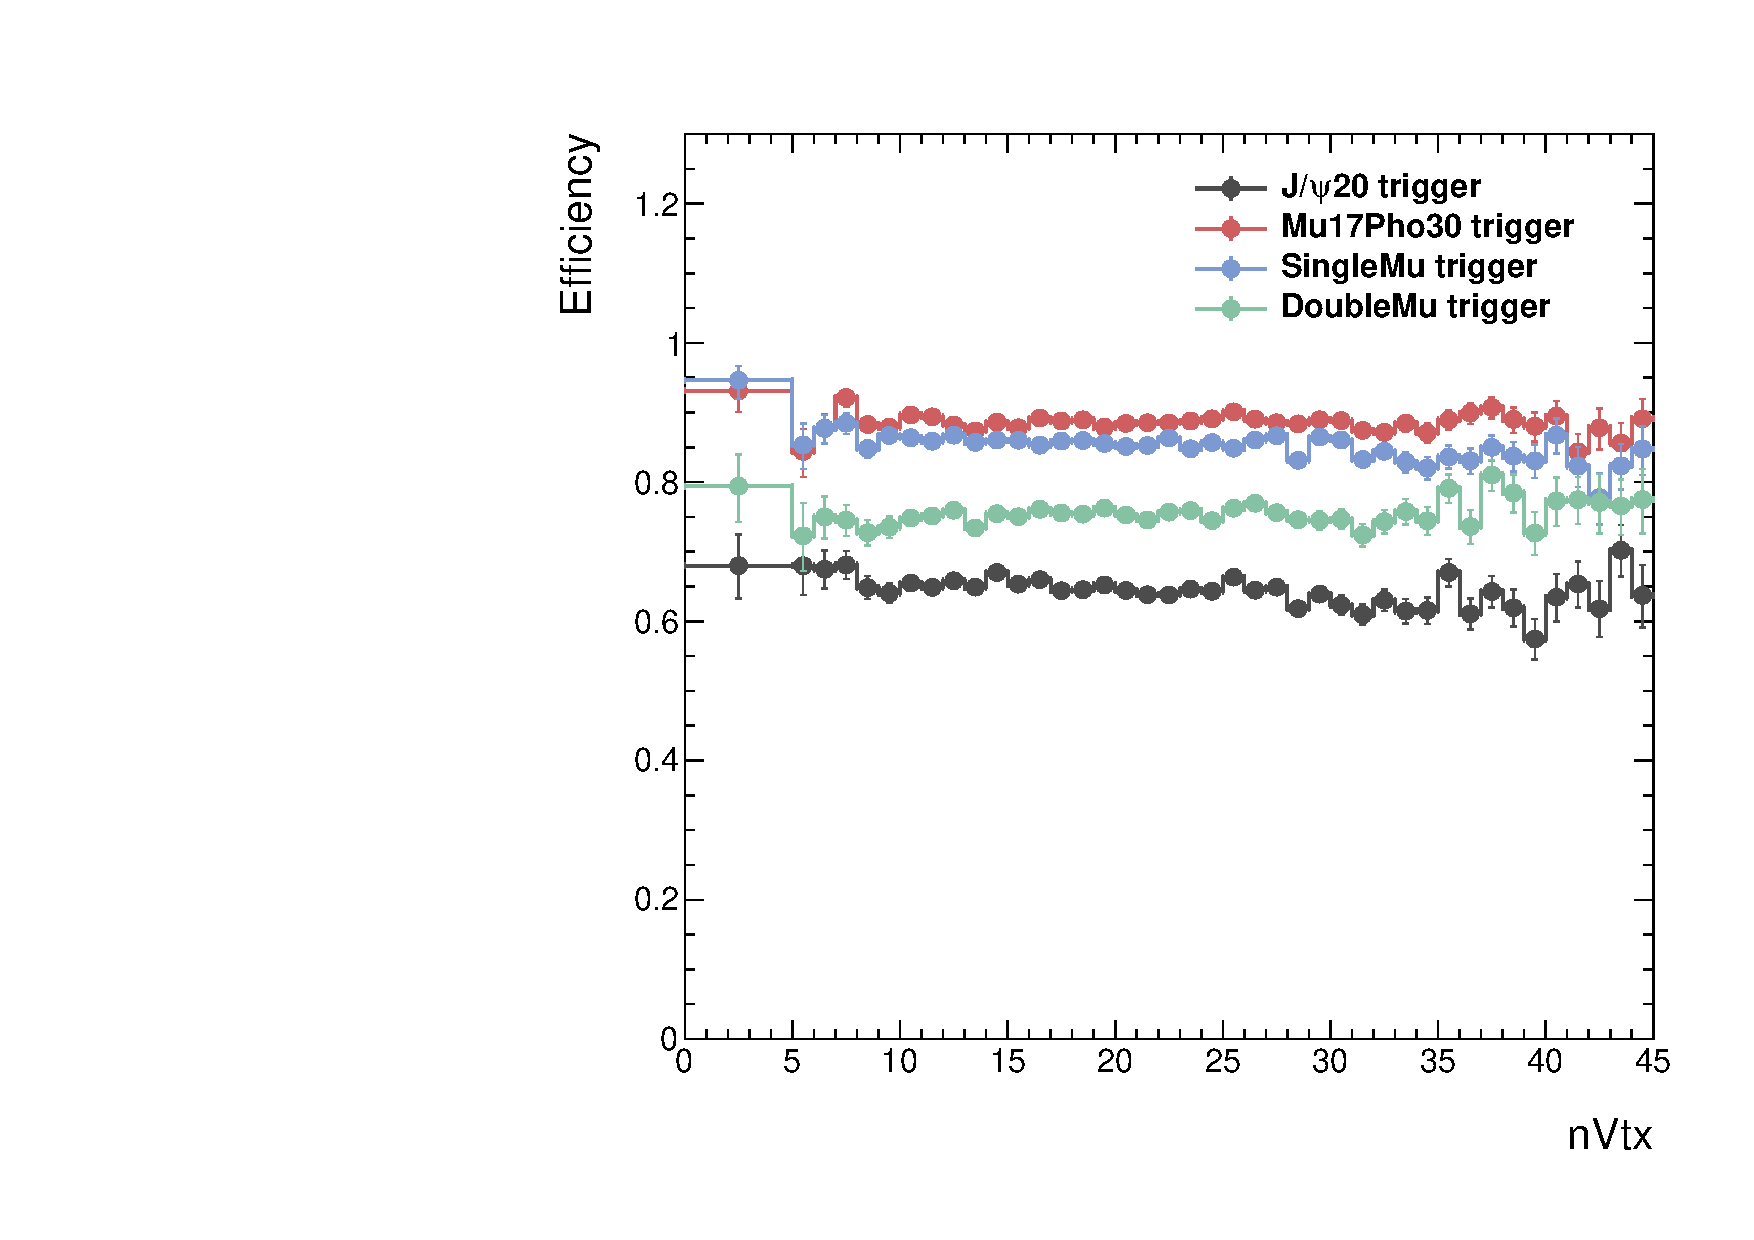
\includegraphics[width=0.45\textwidth]{Fig/Trigger/Eff_nVtx_HJpsiG_Comp}\\
		    \caption{The trigger efficiency in the $\PH\to\JPsi\ \gamma$ signal as function of leading muon $\pt$ (top left), $\pt$ of the dimuon system (top right), photon $\et$ (middle left), angular separation $\Delta R$ between the muons (middle right), invariant mass of the dimuon system $m_{\mu\mu}$ (bottom left), and the number of vertex (bottom right).\label{fig:Trigacceff}}
		\end{figure}
		
		Fig.~\ref{fig:Trigacceff} shows the trigger efficiency in the $\PH\to \JPsi\ \gamma$ signal as function of $\pt$ of the leading muon, $\pt$ of the dimuon system, photon $\et$, angular separation ($\Delta R$) between the muons, invariant mass of the dimuon system $m_{\mu\mu}$, and the number of vertex. As one can see, the muon-photon trigger preserves the highest signal efficiency. The inefficiencies of double muon and quarkonium triggers are responsible for that both triggers are not specifically designed for the muons with small separation. The efficiency of single muon trigger is slightly lower than that of the muon-photon trigger, which may be due to the isolation requirement and high $\pt$ threshold. 
		Consequently, the muon-photon trigger is chosen.   
		
		In the actual signal events, the trigger efficiency is 89.2 (84.2)\% in the Higgs ($\cPZ$) boson decay. The trigger efficiency is measured in the control sample, and found to be 81.5 (83.3)\% in data (simulation). The method of this measurement is described in the next section. 
		
		\subsection*{Trigger efficiency measurement}
		Trigger efficiency in data is measured using $\cPZ\rightarrow\mu\mu\gamma$ control sample in the dataset collected by single muon trigger, while in the simulated events the Drell-Yan jets with $m_{ll} > 50\GeV$ sample is used. Events must have at least two muons and one photon in the final state, and are required to pass at least one of the two single muon triggers, HLT\_MuIso24 or HLT\_MuTkIso24. The muon that fires one or both triggers is considered as the tag muon, and is further required to pass Tight Muon ID and relative isolation requirement~\cite{Sirunyan:2018fpa}. One muon and one photon are then selected as probe objects, and are required to pass the kinematic selections listed below, which ensure that they come from the $\cPZ$ decay with a final-state-radiated (FSR) photon.
		
		\begin{itemize}
		\item $0.1 < \Delta R(\mu ,\gamma) < 0.8$, where the lower bound of 0.1 rejects events where the selected photon picks up the track from one of the muons, and the upper bound of 0.8 rejects events where neither muons emitted the photon
		\item $m_{\mu\mu} + m_{\mu\mu\gamma} < 180\GeV$ to reject contribution from initial-state-radiated (ISR) photons
		\item $60 < m_{\mu\mu\gamma} < 120\GeV$, the mass window cut used to identify the $\cPZ$ boson.
		\end{itemize}
		
		If there are two muons passing tag selections simultanously, we could choose between two possible tag muons. In this case, both choices are considered and tested, and the event is counted twice. This is to avoid underestimating the efficiency and the potential bias on the measurement.
		
	The $\cPZ$ boson cadidate mass distribution in data and MC obtained through this method are shown in Fig.~\ref{fig:Trigplotmass}. Offline selection requirements of the analysis are applied in order to factorize the selection efficiency. The events passing all these selections are counted as the denominator of the trigger efficiency.  For the numerator, the probe muon (photon) is tested to see if it can fire the muon (photon) leg of the muon-photon trigger used in the analysis. 
	The filters in the muon-photon trigger are listed in Table~\ref{table:Filters}. (The filters checked for the muon and photon legs are different between runs B to E and F to H. The filters in the MC sample are the same as those in run F to H in data)
	The filters marked in red color are used for testing the muon leg, while those in blue are for the photon leg. 
		
		There is almost no Run-dependency in trigger efficiency (except for period B), as shown in the red points in Fig. \ref{fig:EffInRun} as well as the constant fits and the resulting $\chi^{2}/\text{ndf}$. The black points shown here, which serve as a reference, are the efficiencies with the standard loose muon ID with additional $\text{d}_{\cPZ}$ and $\text{d}_{\text{xy}}$ cuts used previously in this analysis.  
		
		\begin{figure}[p]
		  \centering
		    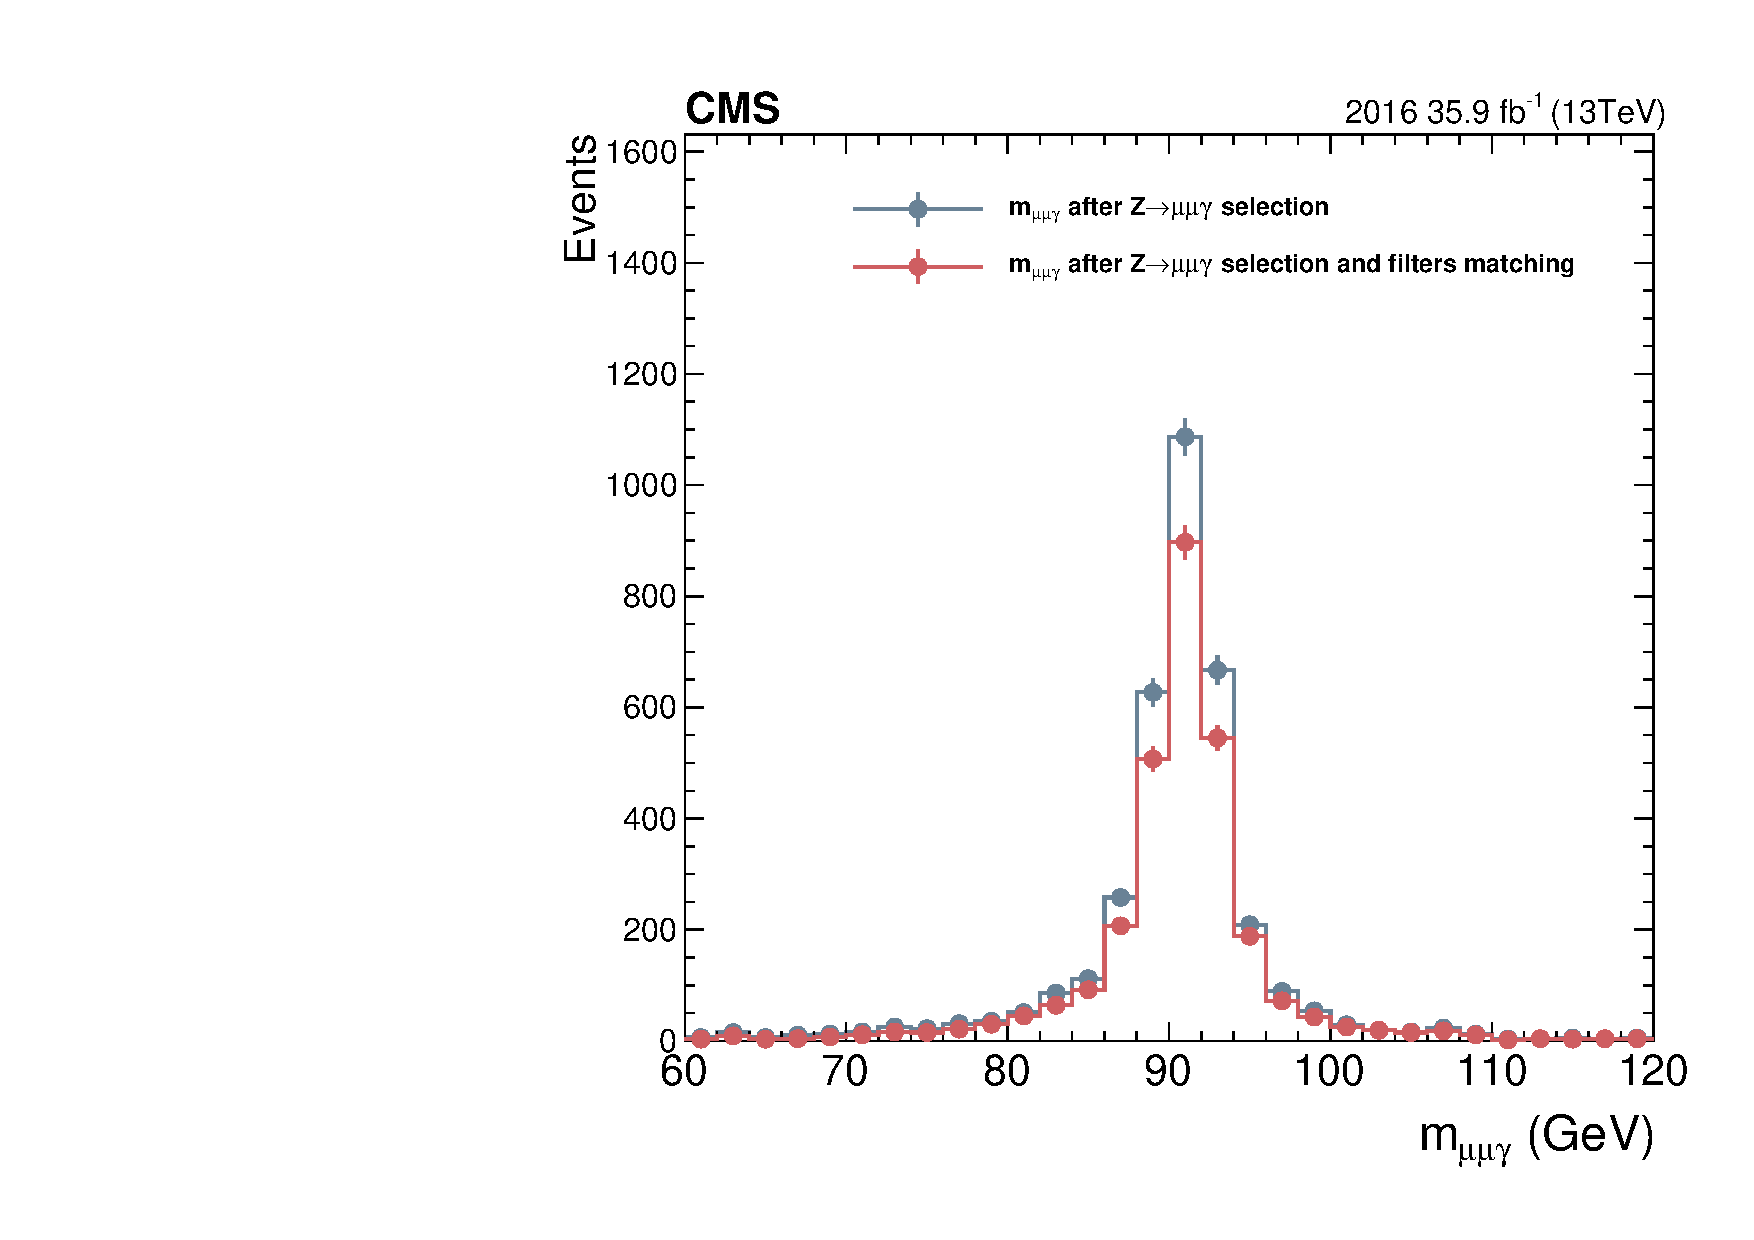
\includegraphics[width=0.7\textwidth]{Fig/Trigger/Kinematics/m_mumugamma_data}\\
		    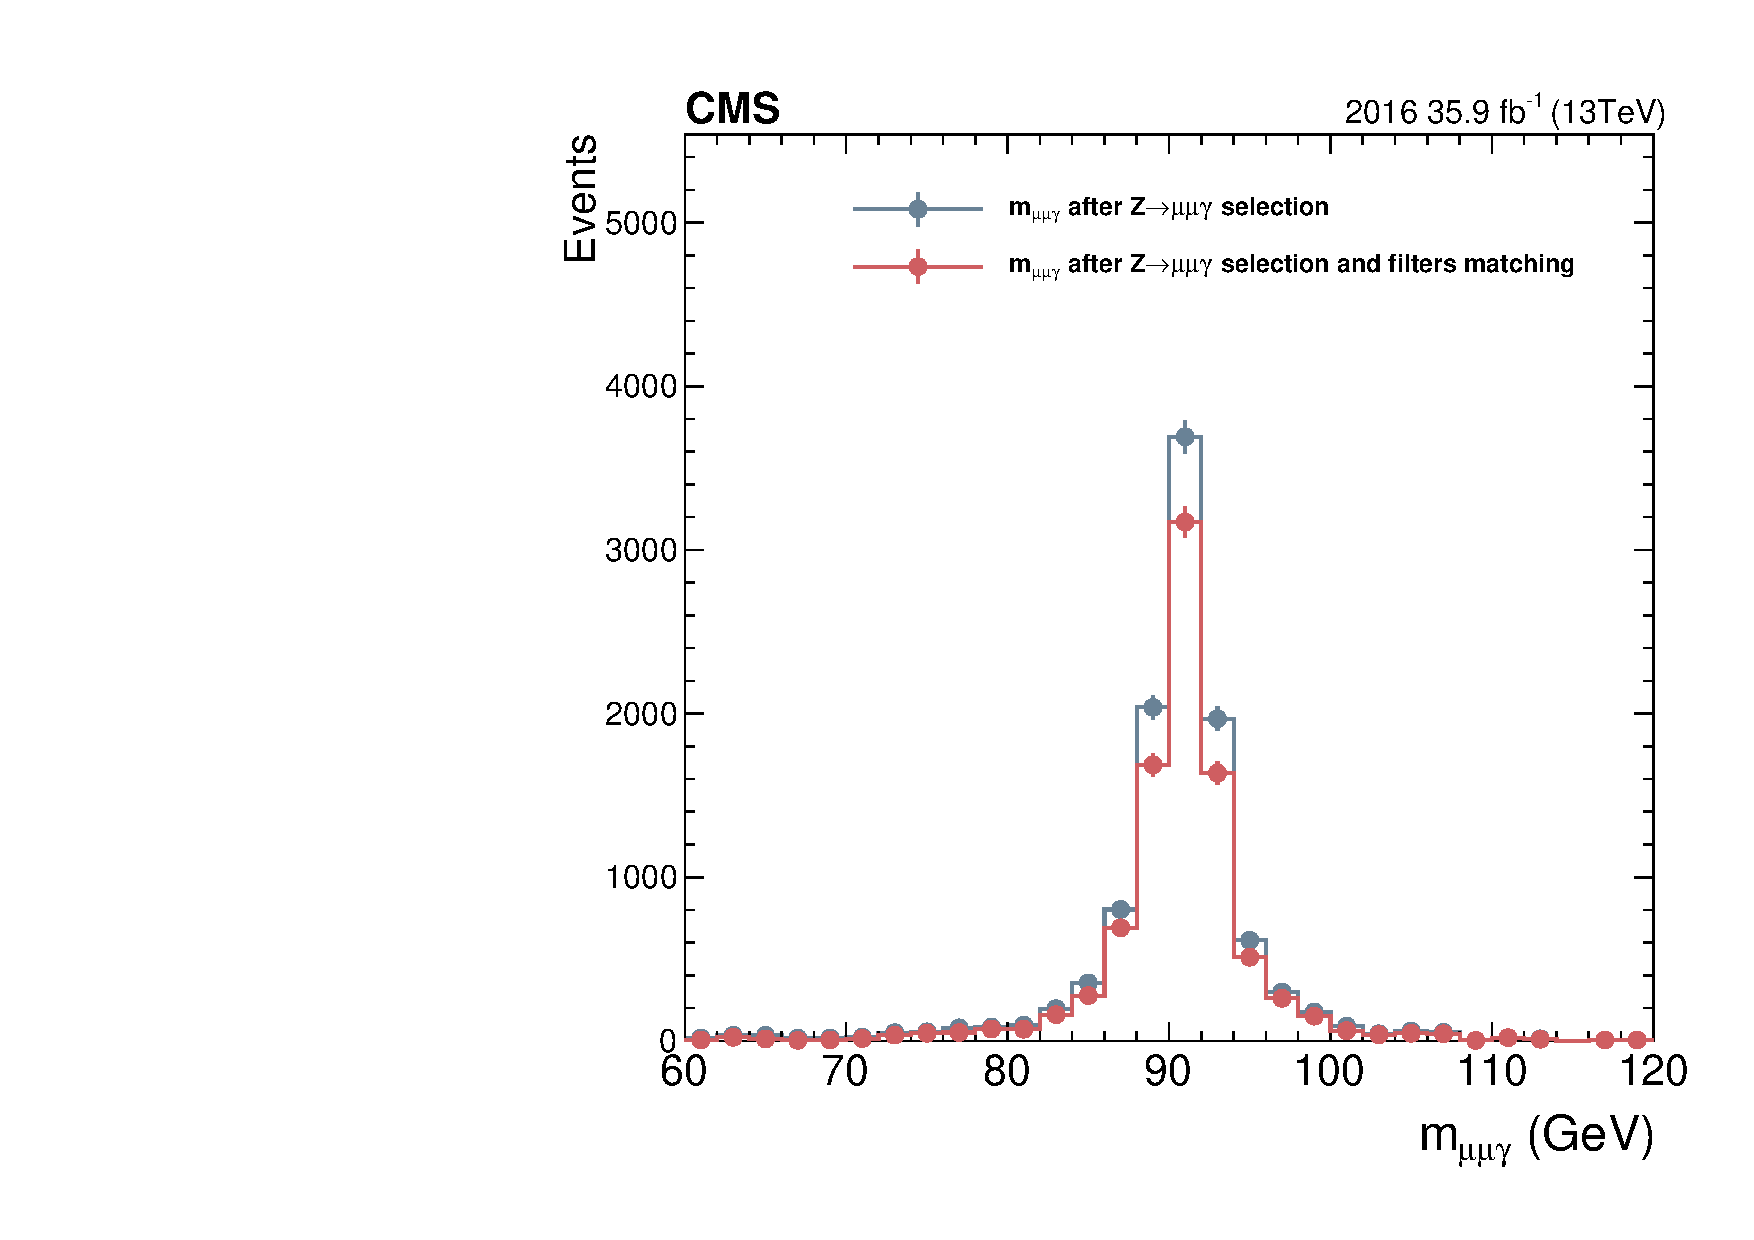
\includegraphics[width=0.7\textwidth]{Fig/Trigger/Kinematics/m_mumugamma_MC_DYJetsToLL_aMCatNLO}\\
		    \caption[Muon SFs]{
		        The $\cPZ$ boson candidate mass after selection in data(top) and MC(bottom).\label{fig:Trigplotmass}}
		\end{figure}
		
		\begin{table}[p]
		\begin{center}
		\begin{tabular}{ |c|c| } 
		  
		\hline
		                  & \textbf{HLT\_Mu17\_Photon30\_CaloIdL\_L1ISO\_v6} \\
		\hline
		                  & Run B$\sim$E \\
		\hline
		 Filters  &  hltL1sMu5IsoEG18\\
		                  &  hltPreMu17Photon30CaloIdLL1ISO\\
		                  &  hltL1fL1sMu5IsoEG18L1Filtered5\\
		                  &  hltL2fL1sL1Mu5IsoEG18L1f5L2Filtered7\\
		                  &  \color{red} hltL3fL1sL1Mu5IsoEG18L1f5L2f7L3Filtered17\\
		                  &  hltEgammaCandidates\\
		                  &  hltEGL1Mu5IsoEG18Filter\\
		                  &  hltMu17Photon30CaloIdLL1ISOEtFilter\\
		                  &  hltEgammaClusterShape\\
		                  &  hltMu17Photon30CaloIdLL1ISOClusterShapeFilter\\
		                  &  hltEgammaHoverE\\
		                  &  \color{blue} hltMu17Photon30CaloIdLL1ISOHEFilter\\
		  \hline
		  \hline
		                  & \textbf{HLT\_Mu17\_Photon30\_CaloIdL\_L1ISO\_v9} \\
		\hline
		                  & RunF$\sim$H, MC samples\\
		\hline
		Filters  &  hltL1sMu5IsoEG18IorMu5IsoEG20\\
		                  &  hltPreMu17Photon30CaloIdLL1ISO\\
		                  &  hltL1fL1sMu5IsoEG18ORMu5IsoEG20L1Filtered5\\
		                  &  hltL2fL1sL1Mu5IsoEG18ORL1Mu5IsoEG20L1f5L2Filtered7\\
		                  &  \color{red} hltL3fL1sL1Mu5IsoEG18ORL1Mu5IsoEG20L1f5L2f7L3Filtered17\\
		                  &  hltEgammaCandidates\\
		                  &  hltEGL1Mu5IsoEG18ORMu5IsoEG20Filter\\
		                  &  hltMu17Photon30CaloIdLL1ISOOREtFilter\\
		                  &  hltEgammaClusterShape\\
		                  &  hltMu17Photon30CaloIdLL1ISOORClusterShapeFilter\\
		                  &  hltEgammaHoverE\\
		                  &  \color{blue} hltMu17Photon30CaloIdLL1ISOORHEFilter\\
		 \hline
		\end{tabular}
		\caption[Filters]{
		 Filters in the muon-photon trigger, listed in sequence. The filters marked in red
		 color are used for testing the muon leg, while those in blue are for the photon leg.  \label{table:Filters}}
		%\end{sideways}  
		\end{center}                                                                                                                                       
		\end{table} 
		
		\begin{figure}[p]
		  \centering
		    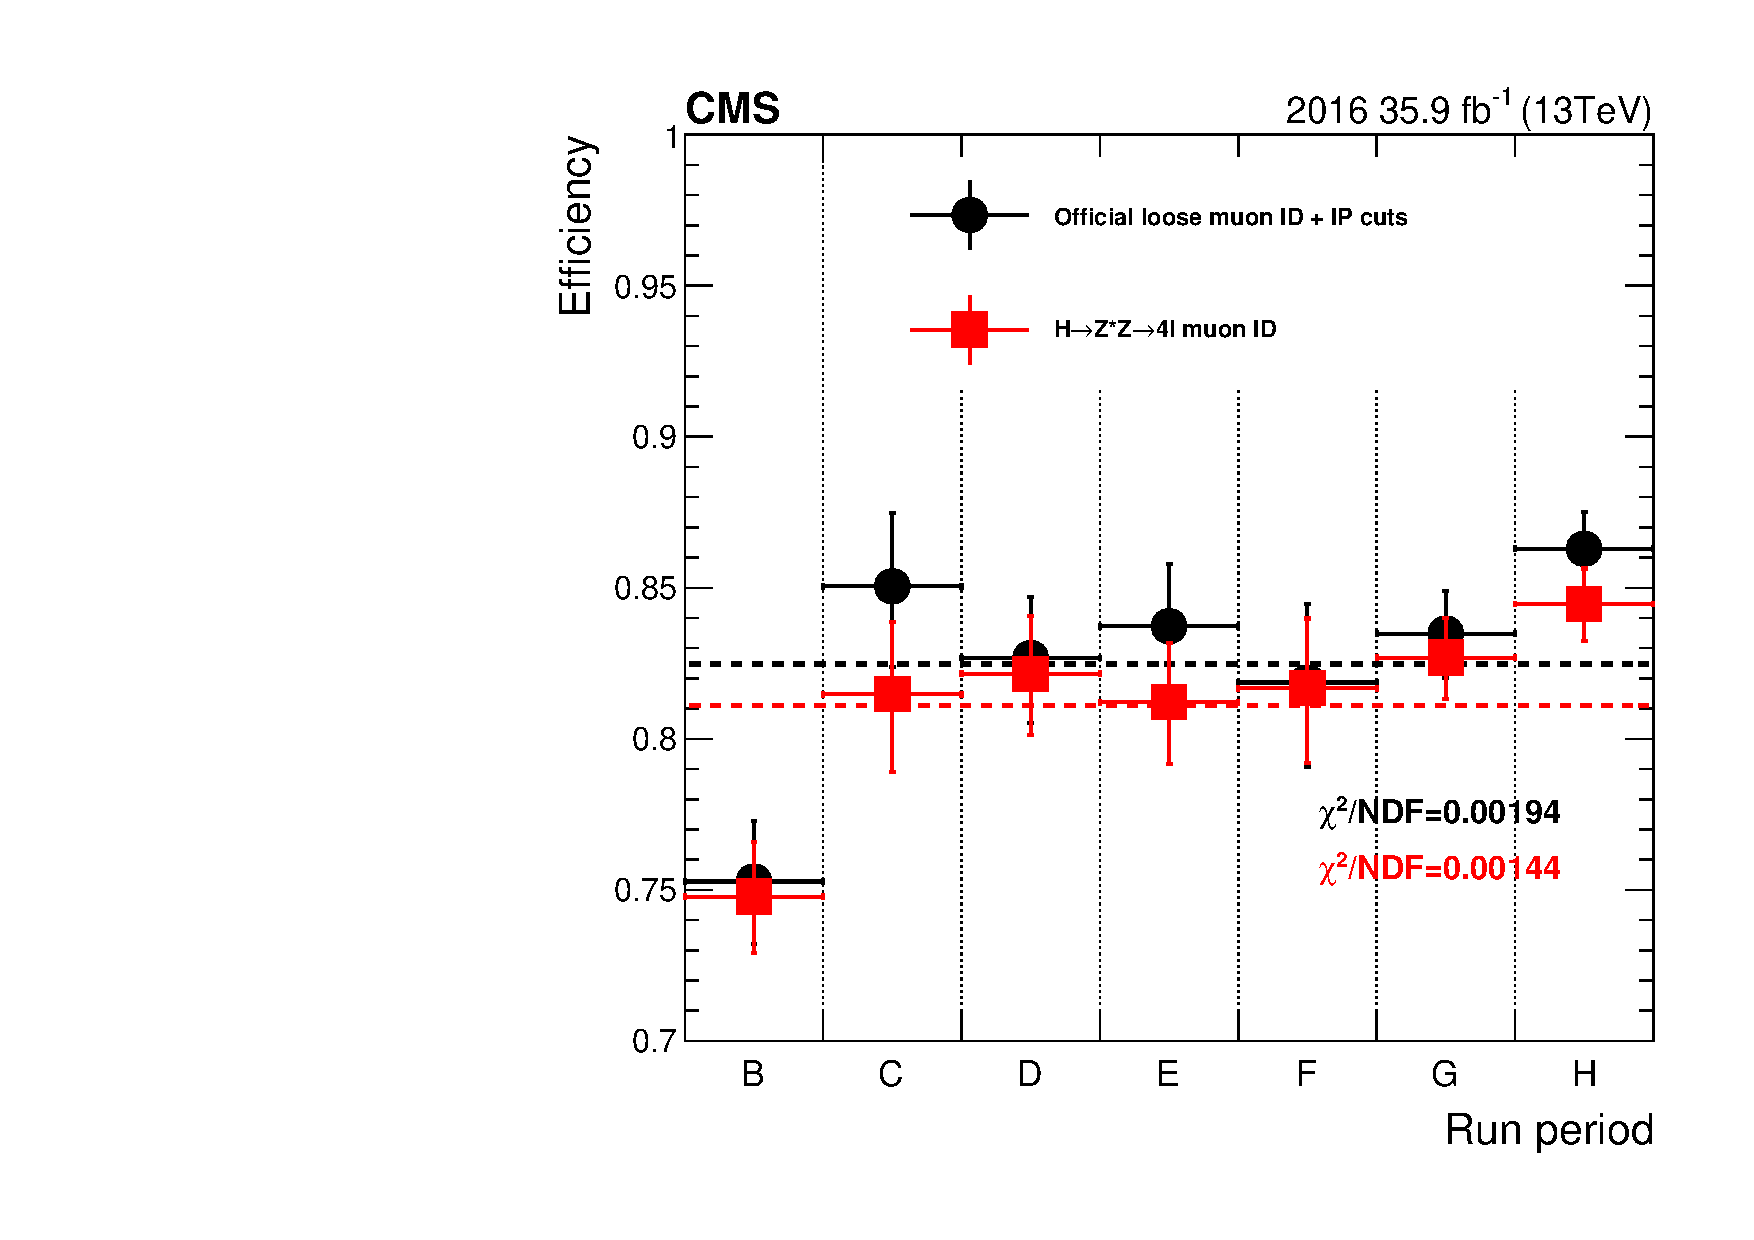
\includegraphics[width=0.7\textwidth]{Fig/Trigger/EffByRuns_HZZ}\\
		    \caption{\label{fig:EffInRun}
		        Trigger efficiency in each run period. Points in black correspond to the efficiencies measured when using the standard loose muon ID with additional $\text{d}_{\cPZ}$ and $\text{d}_{\text{xy}}$ cuts used previously in this analysis, while red points correspond to the efficiencies measured using the muon ID optimized for $\PH\rightarrow \cPZ\cPZ^{*}\rightarrow 4\text{l}$ analysis that is currently used.}
		\end{figure}
		
		Trigger efficiency as a function of probe photon $\et$, probe muon $\pt$, probe muon psudorapidity $\eta^{\mu}$, and probe photon supercluster psudorapidity $\eta_{SC}^{\gamma}$ are shown in Fig.~\ref{fig:Trigploteff}. The efficiency as function of probe muon $\pt$ is made with the probe photon $\et > 33\GeV$. Similarly, the plot as function of probe photon $\et$ is made with the probe muon $\pt > 20\GeV$. 
		
	The trigger efficiency scale factors -- the ratio of Data/MC	 efficiencies -- are to be applied to simulated samples.  They are derived in bins of probe muon $\pt$ and probe photon $\et$ in 2 photon supercluster eta $\eta_{SC}$ regions : Ecal Barrel (EB) region ($0 < \eta_{SC} < 1.4442$) and Ecal Endcap (EE) region ($1.566 < \eta_{SC} < 2.5$).  
	When applying the trigger efficiency scale factors to MC samples, it is assumed that the leading muon is the one that fires the muon leg of the trigger, so the leading muon $\pt$ and photon $\et$ are used to determine which trigger efficiency bin to apply on an event. 
	Results for the trigger efficiency measurement are shown in Fig.~\ref{fig:TrigEffsep} and the scale factors are shown in Fig.~\ref{fig:TrigEff}. The uncertainty of each bin on Fig.~\ref{fig:TrigEffsep} only includes statistical uncertainty, while uncertainties shown in Fig.~\ref{fig:TrigEff} are total systematic uncertainties, which will be detailed in Section~\ref{sec:Systematic}.
		
		\begin{figure}[p]
		  \centering
		    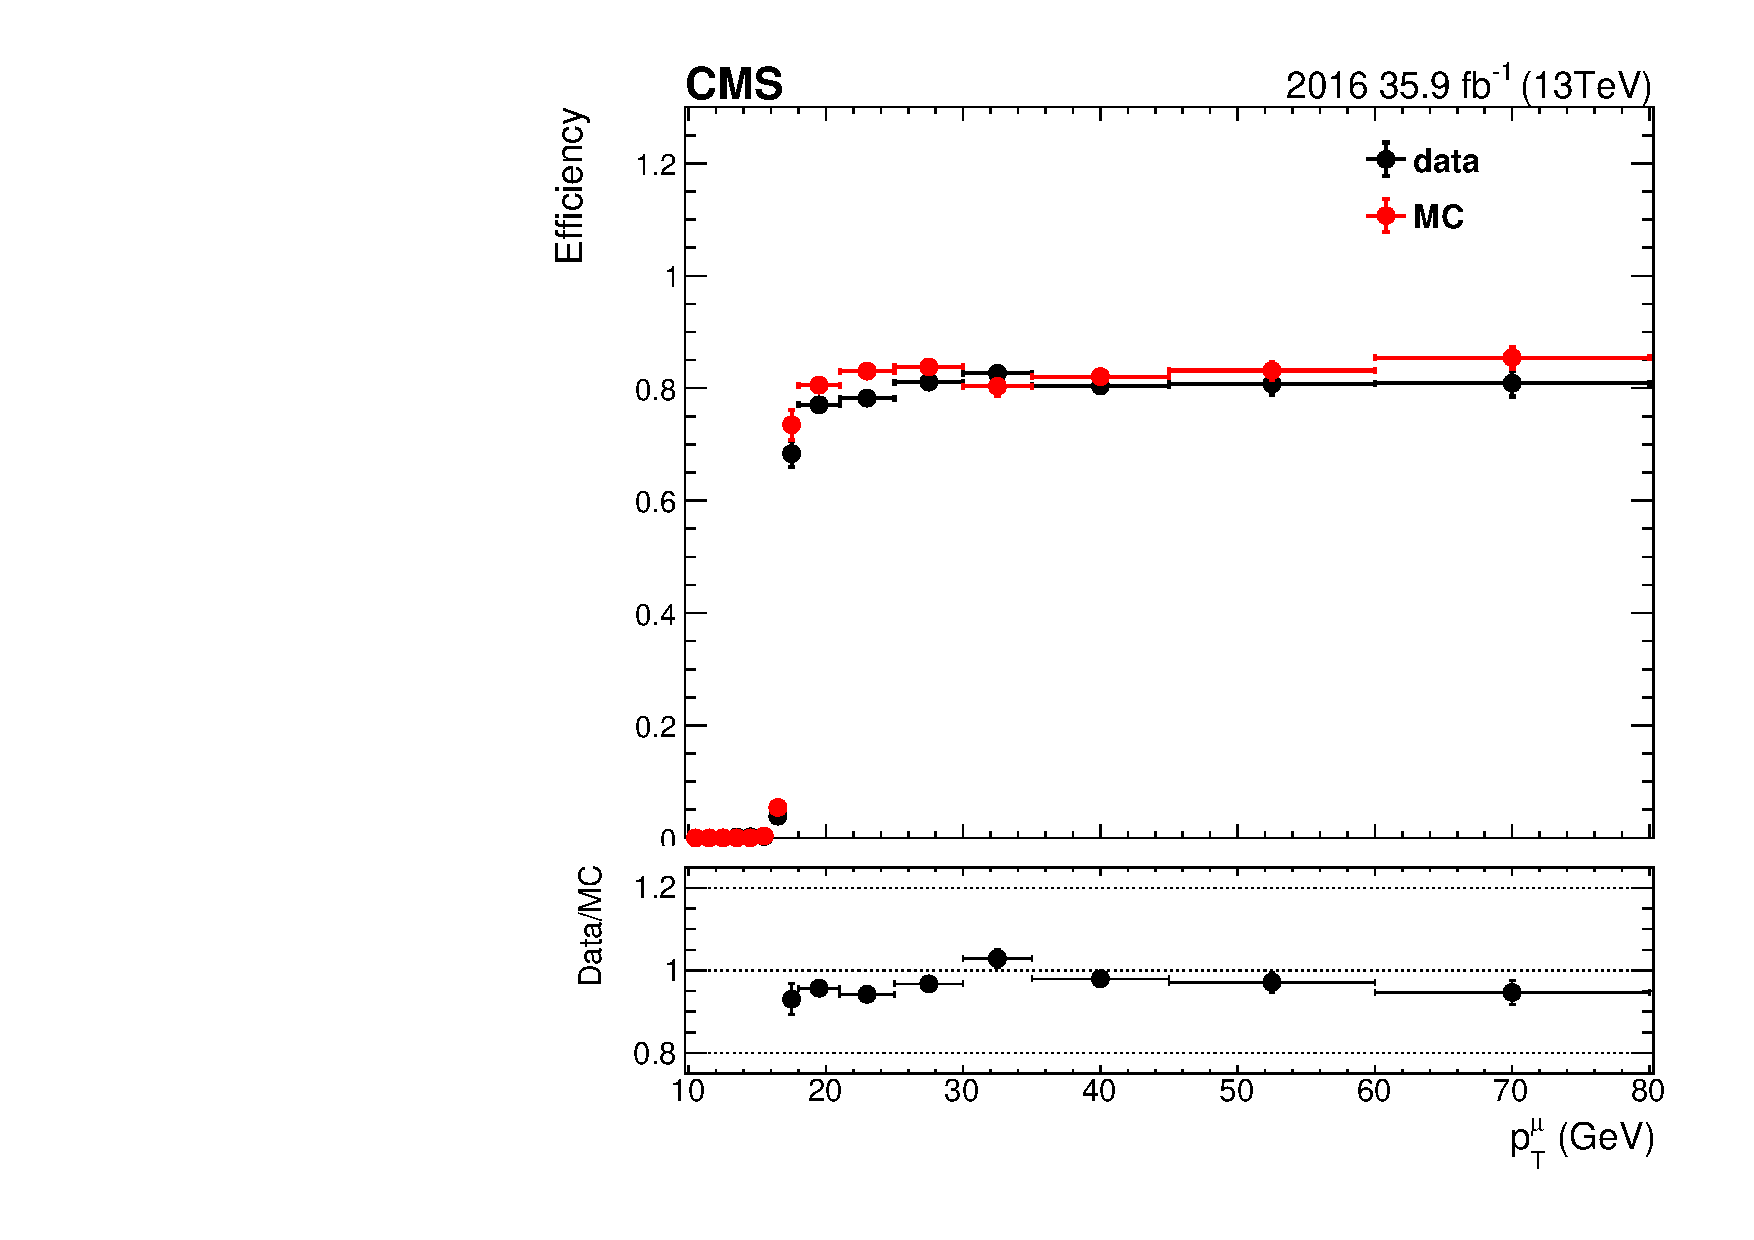
\includegraphics[width=0.47\textwidth]{Fig/Trigger/Eff_1D/Eff_ProbeMuonPt_DYJetsToLL_aMCatNLO}~
		    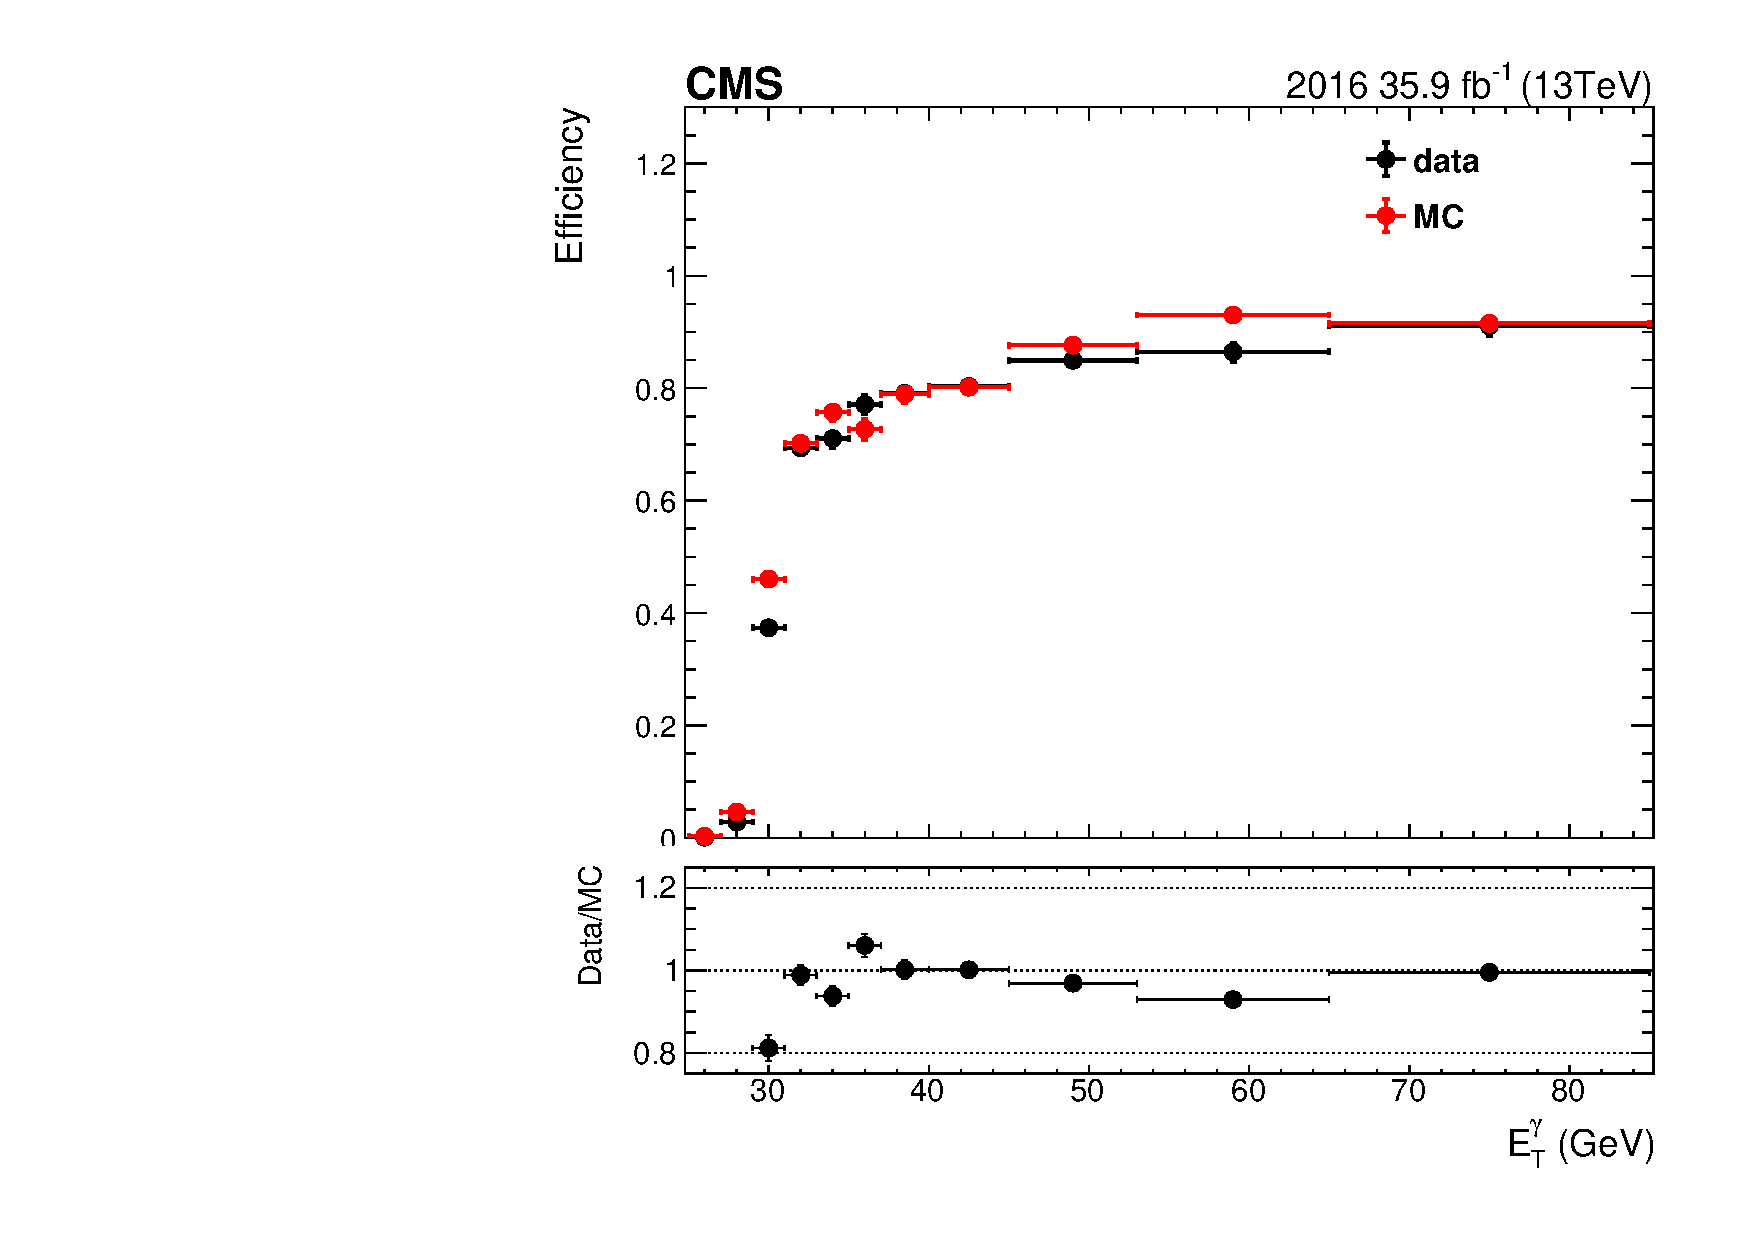
\includegraphics[width=0.47\textwidth]{Fig/Trigger/Eff_1D/Eff_ProbePhotonEt_DYJetsToLL_aMCatNLO}\\
		    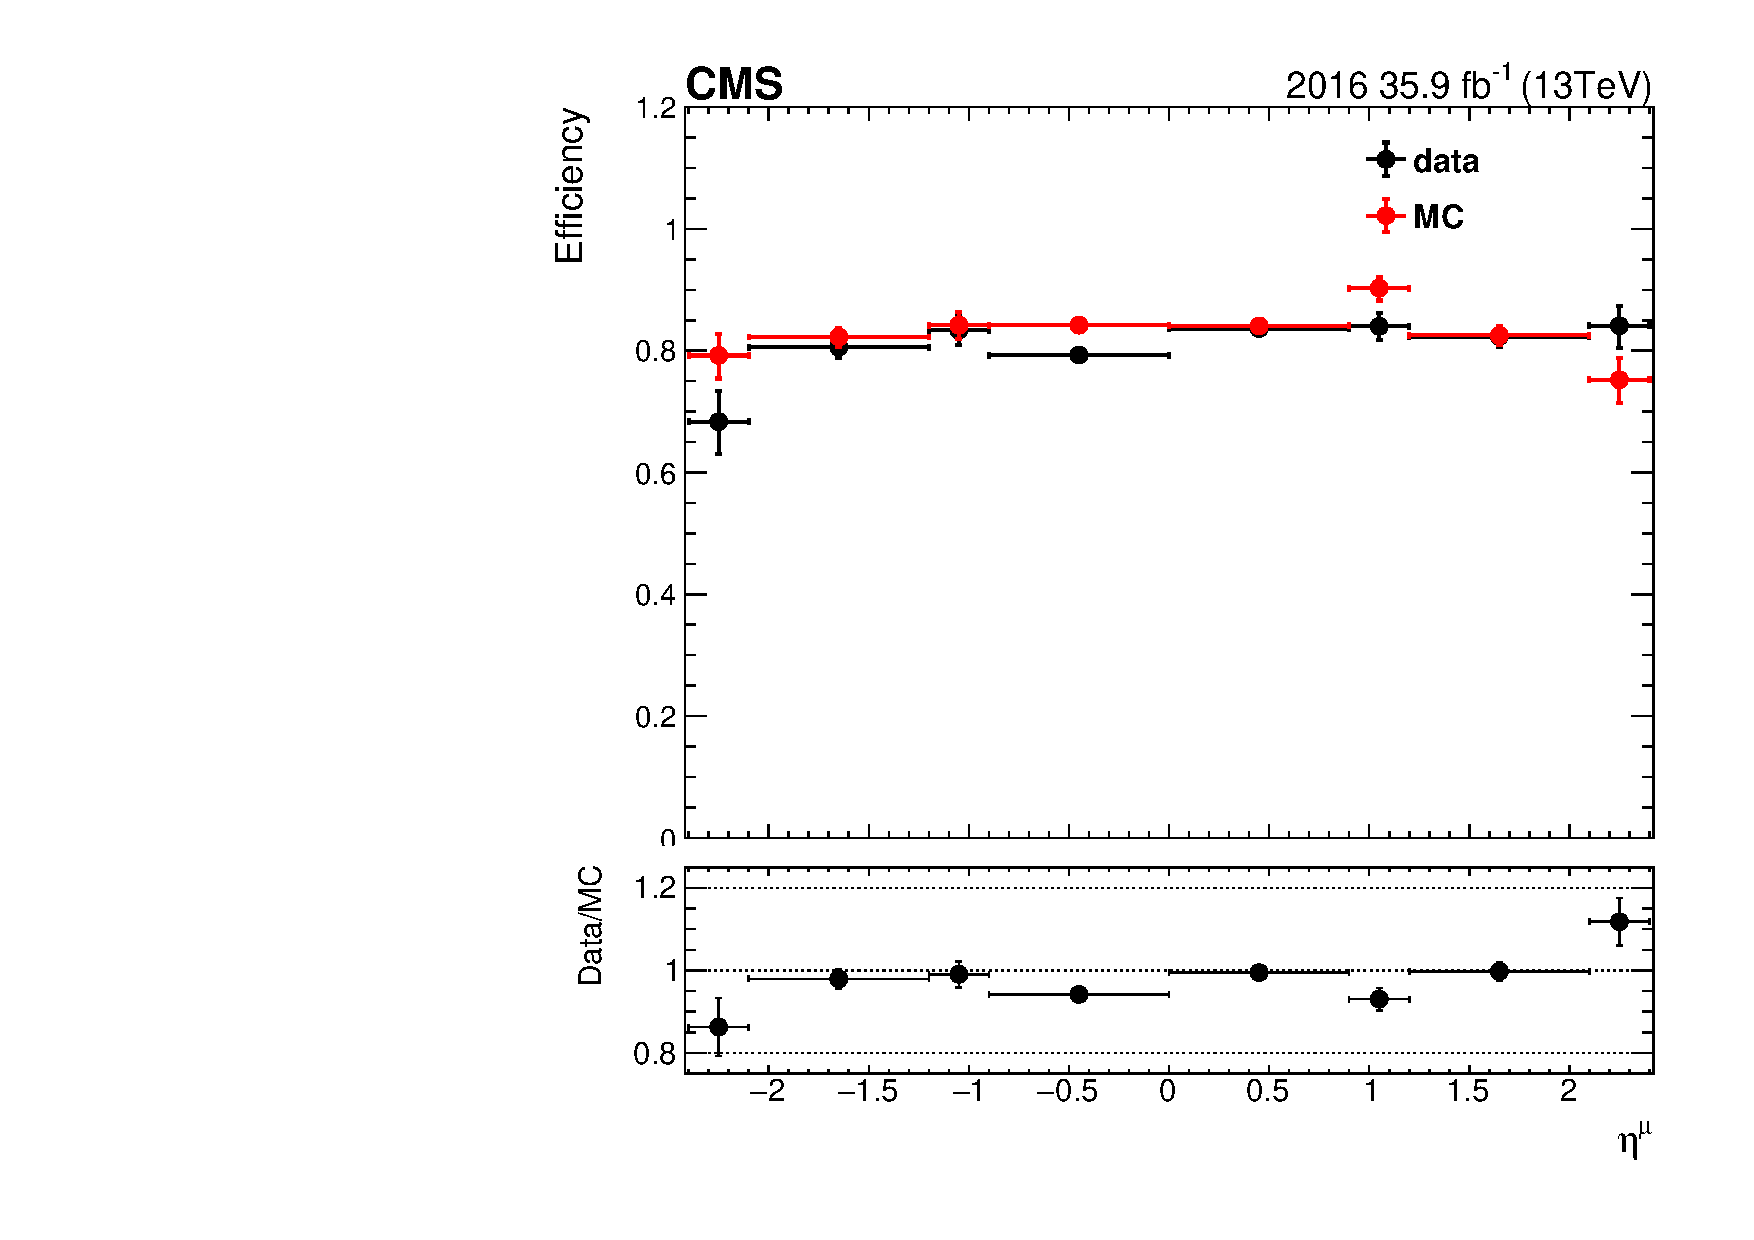
\includegraphics[width=0.47\textwidth]{Fig/Trigger/Eff_1D/Eff_ProbeMuonEta_DYJetsToLL_aMCatNLO}~
		    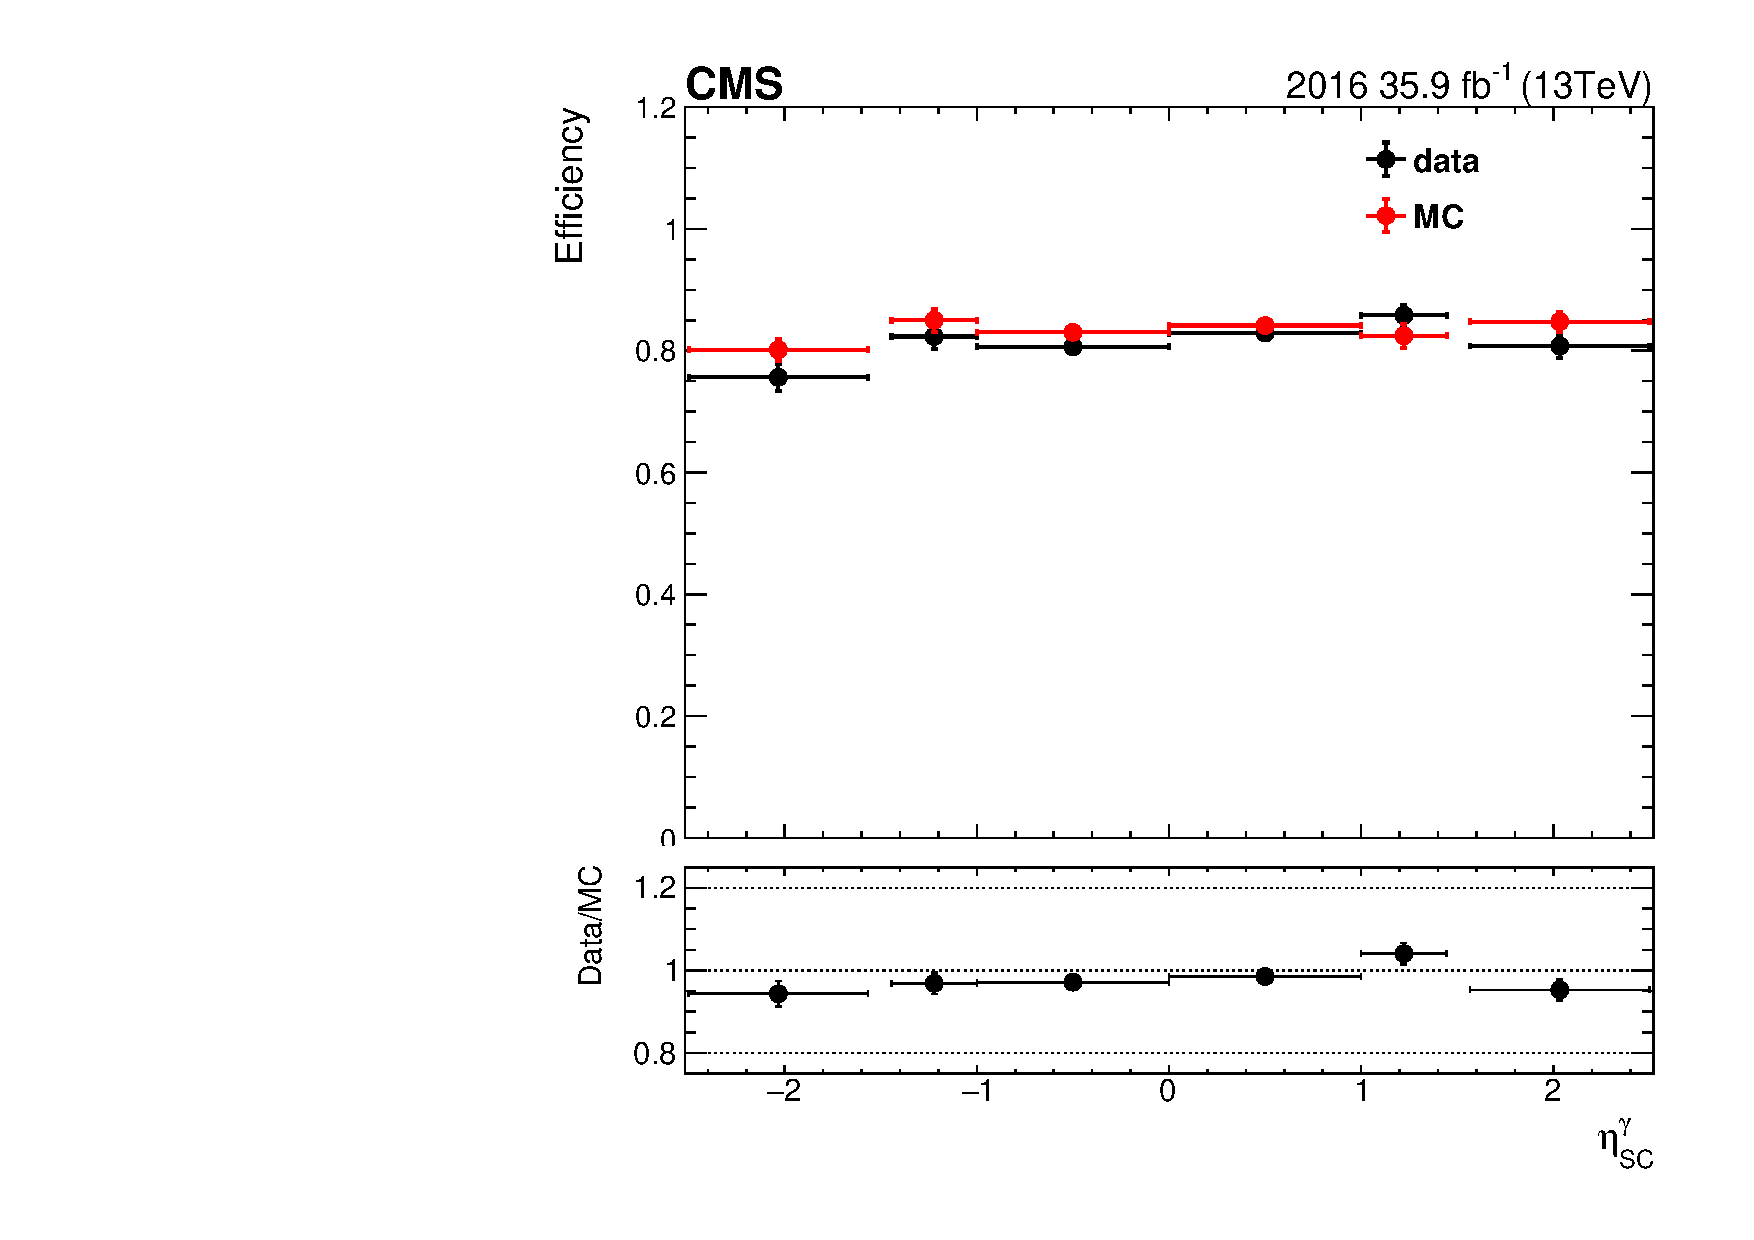
\includegraphics[width=0.47\textwidth]{Fig/Trigger/Eff_1D/Eff_ProbePhotonSCEta_DYJetsToLL_aMCatNLO} \\
		    \caption[TrigEff PtEta]{Trigger efficiency as a function of probe muon $\pt$ (top left), probe photon $\et$ (top right), probe muon $\pt$ (bottom left), and probe photon $\eta^{SC}$ (Bottom right).}
		    \label{fig:Trigploteff}
		\end{figure}
		
		\begin{figure}[p]
		  \centering
		    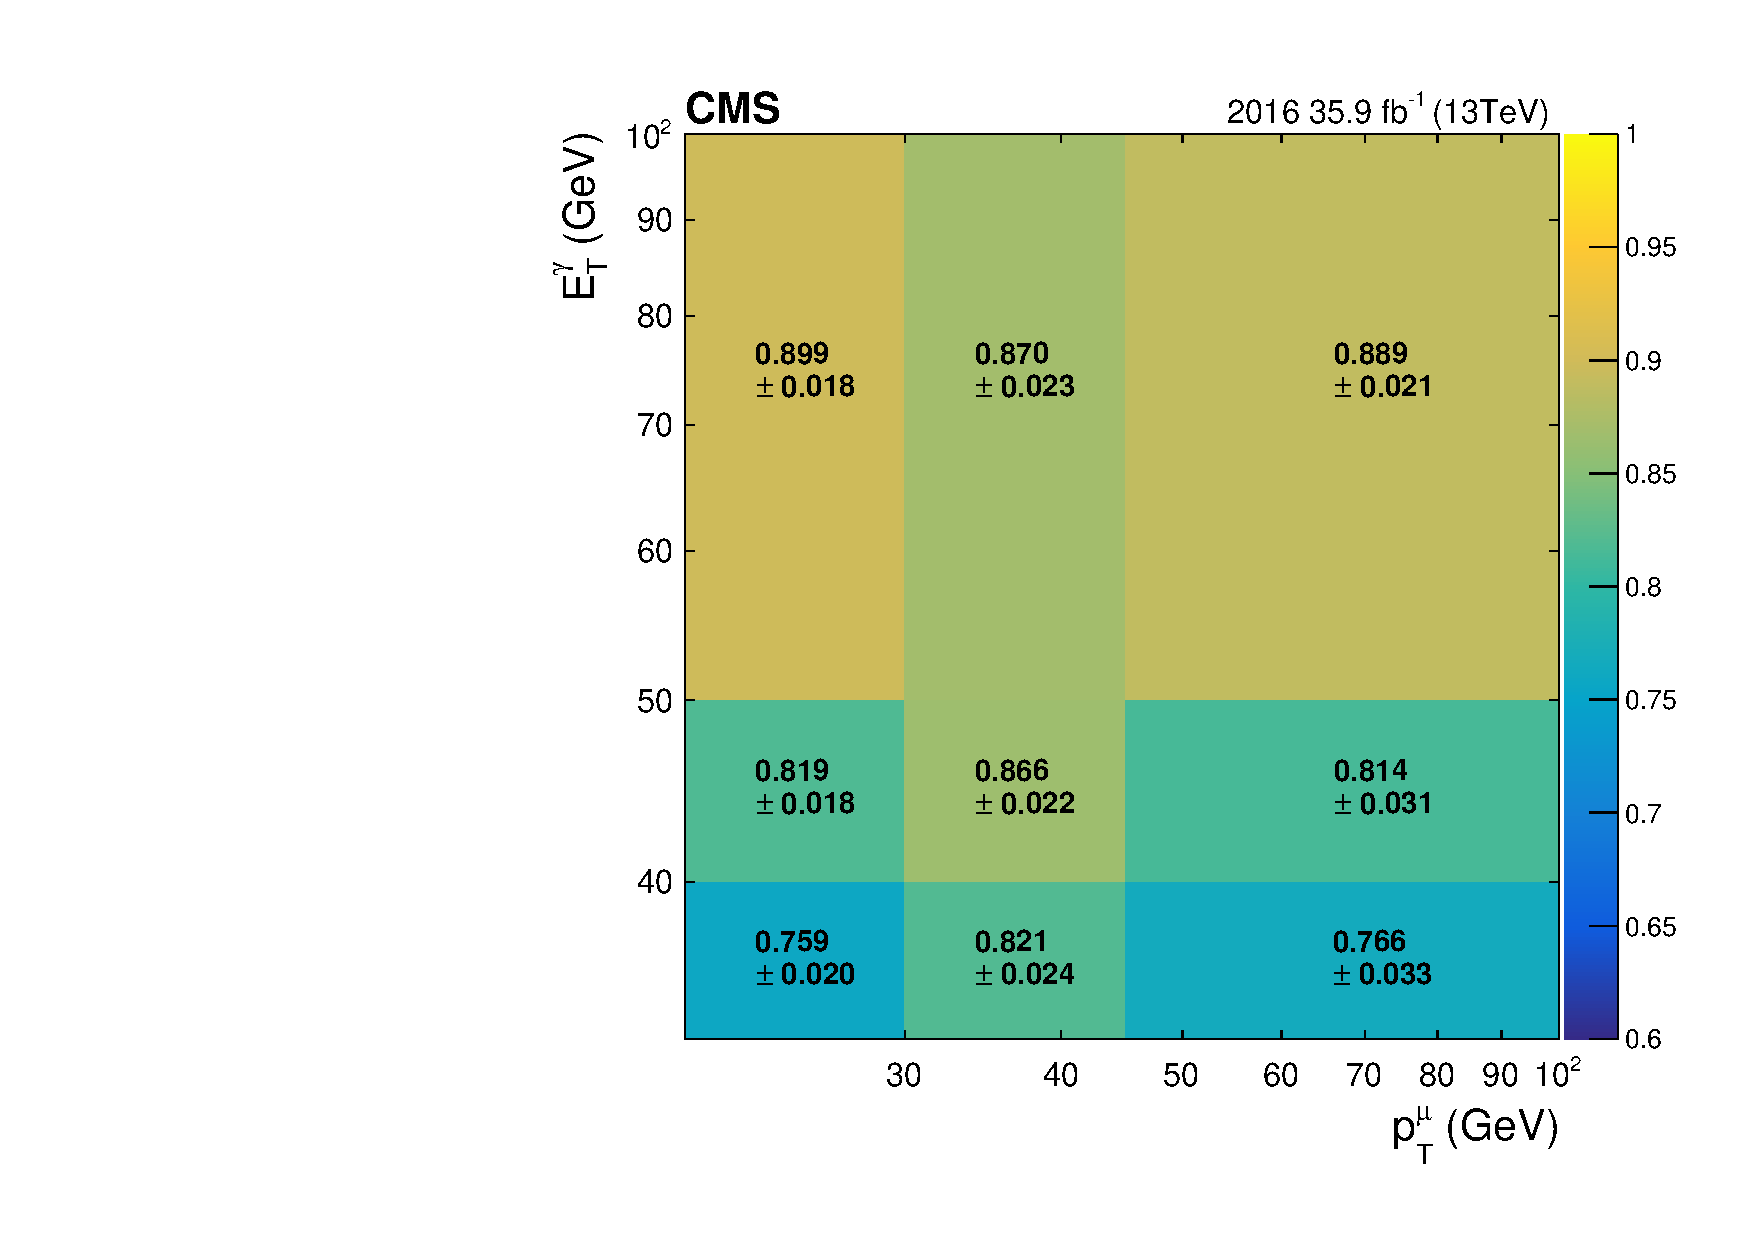
\includegraphics[width=0.47\textwidth]{Fig/Trigger/HZZID/Efficiency_MuPt_PhoEt_EB_data}~
		    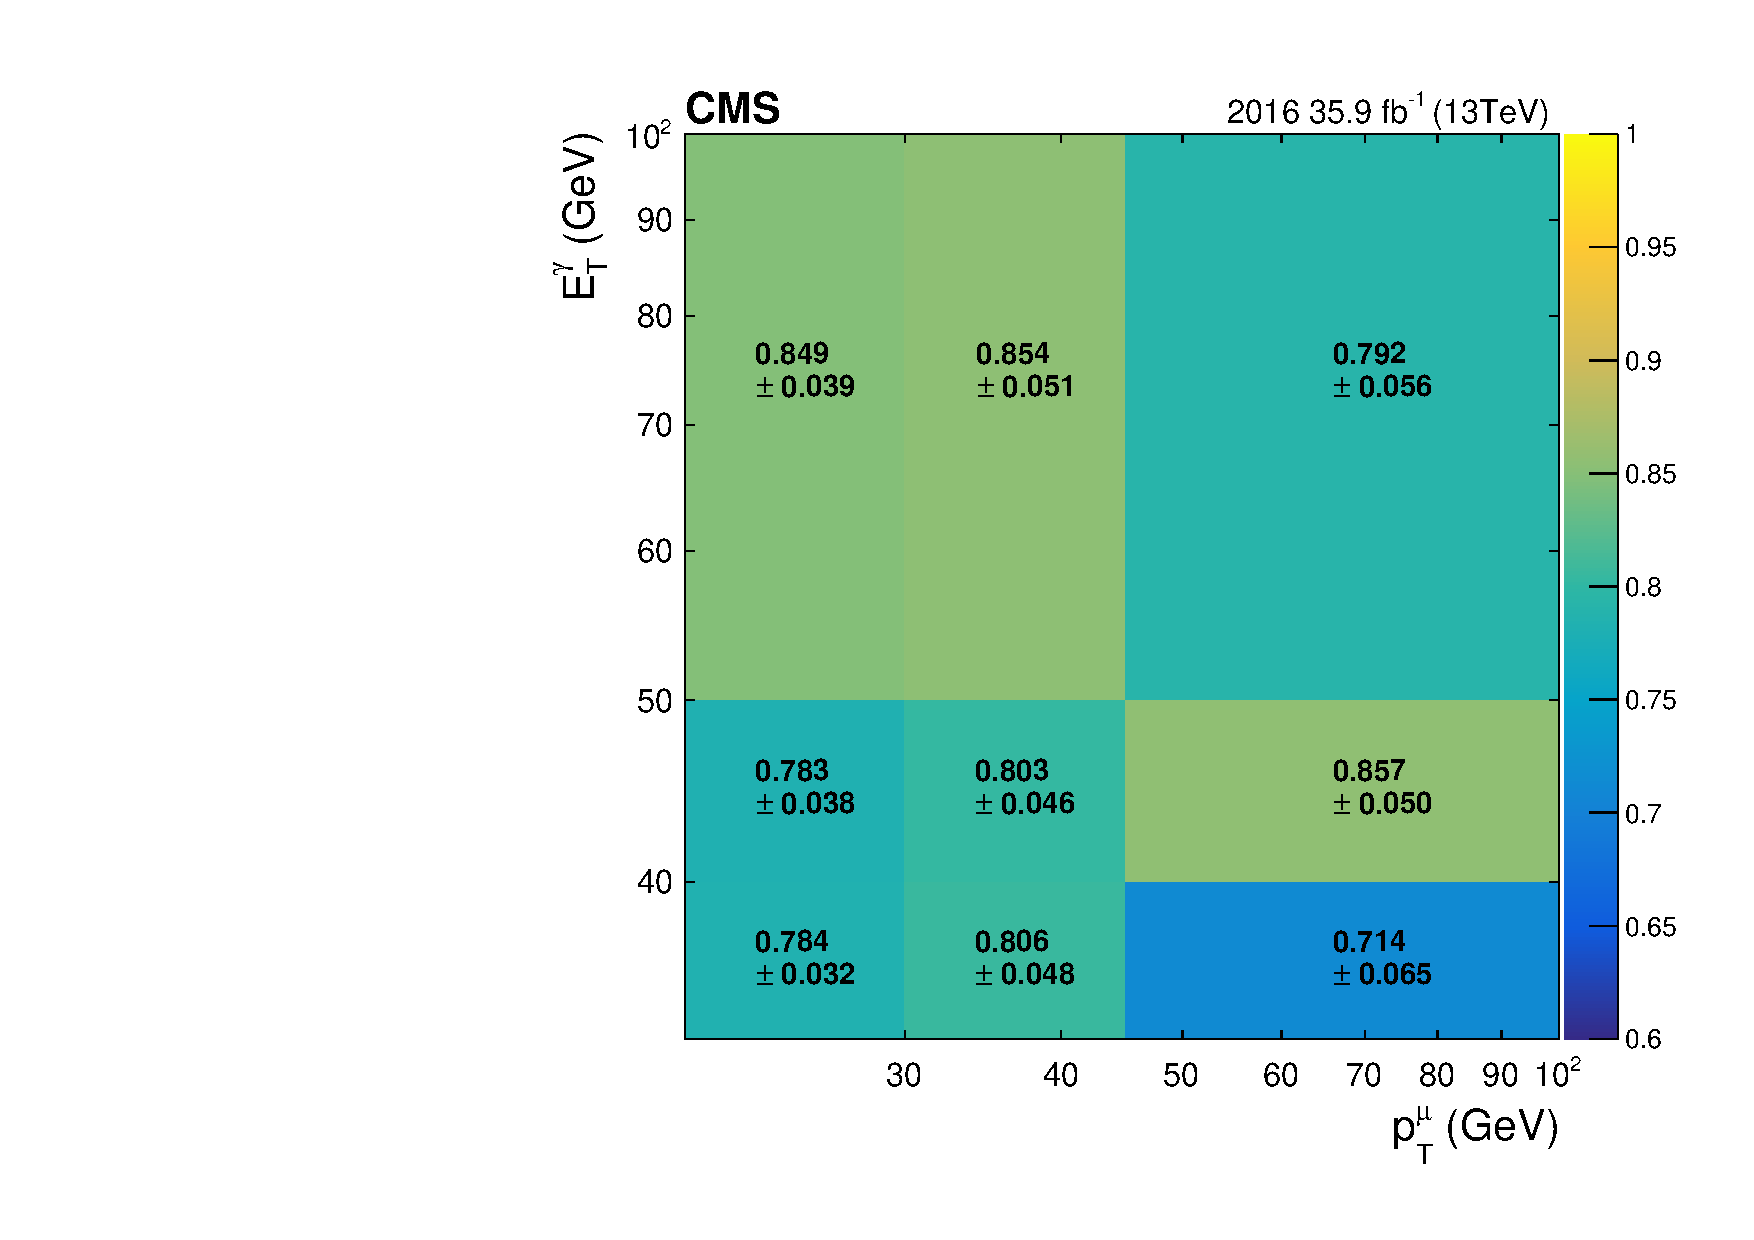
\includegraphics[width=0.47\textwidth]{Fig/Trigger/HZZID/Efficiency_MuPt_PhoEt_EE_data}\\
		    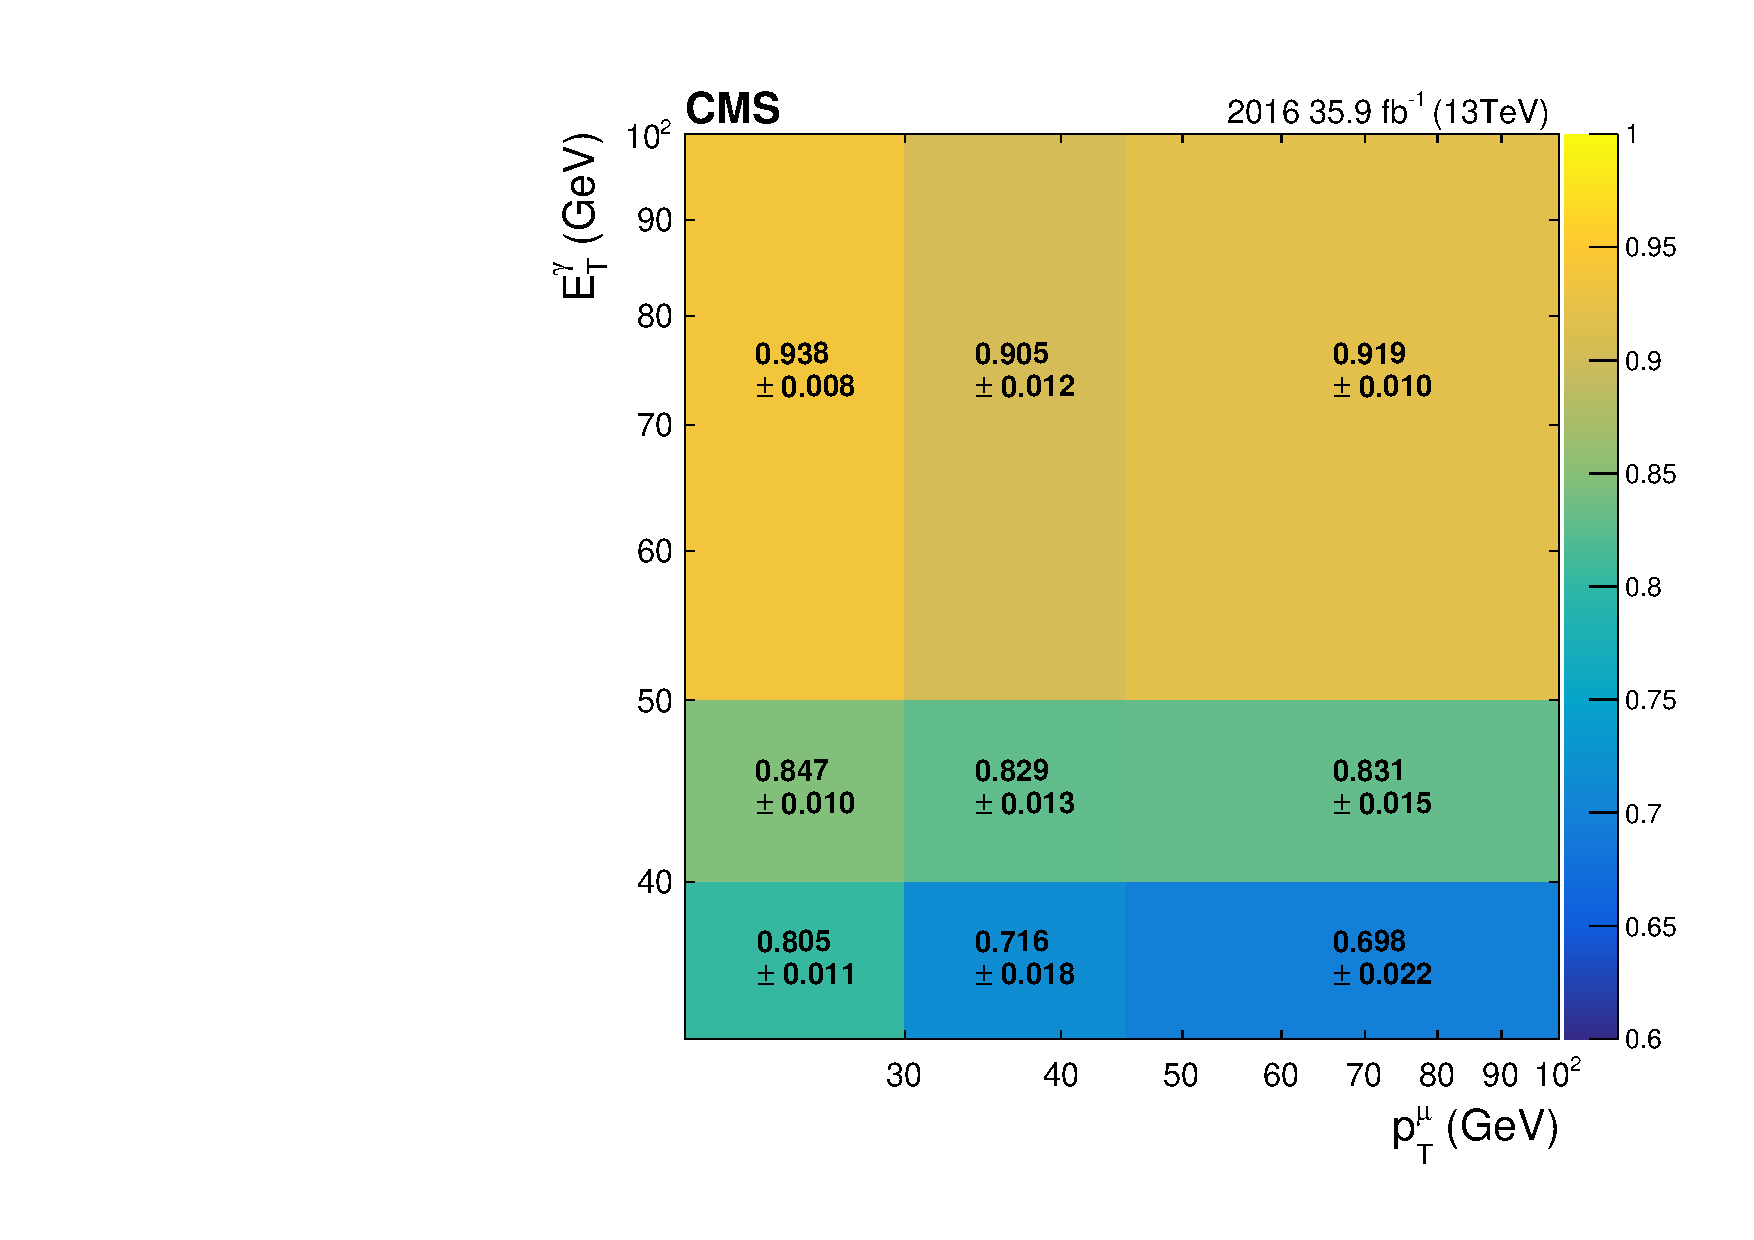
\includegraphics[width=0.47\textwidth]{Fig/Trigger/HZZID/Efficiency_MuPt_PhoEt_MC_DYJetsToLL_aMCatNLO_PU_nominal_EB}~
		    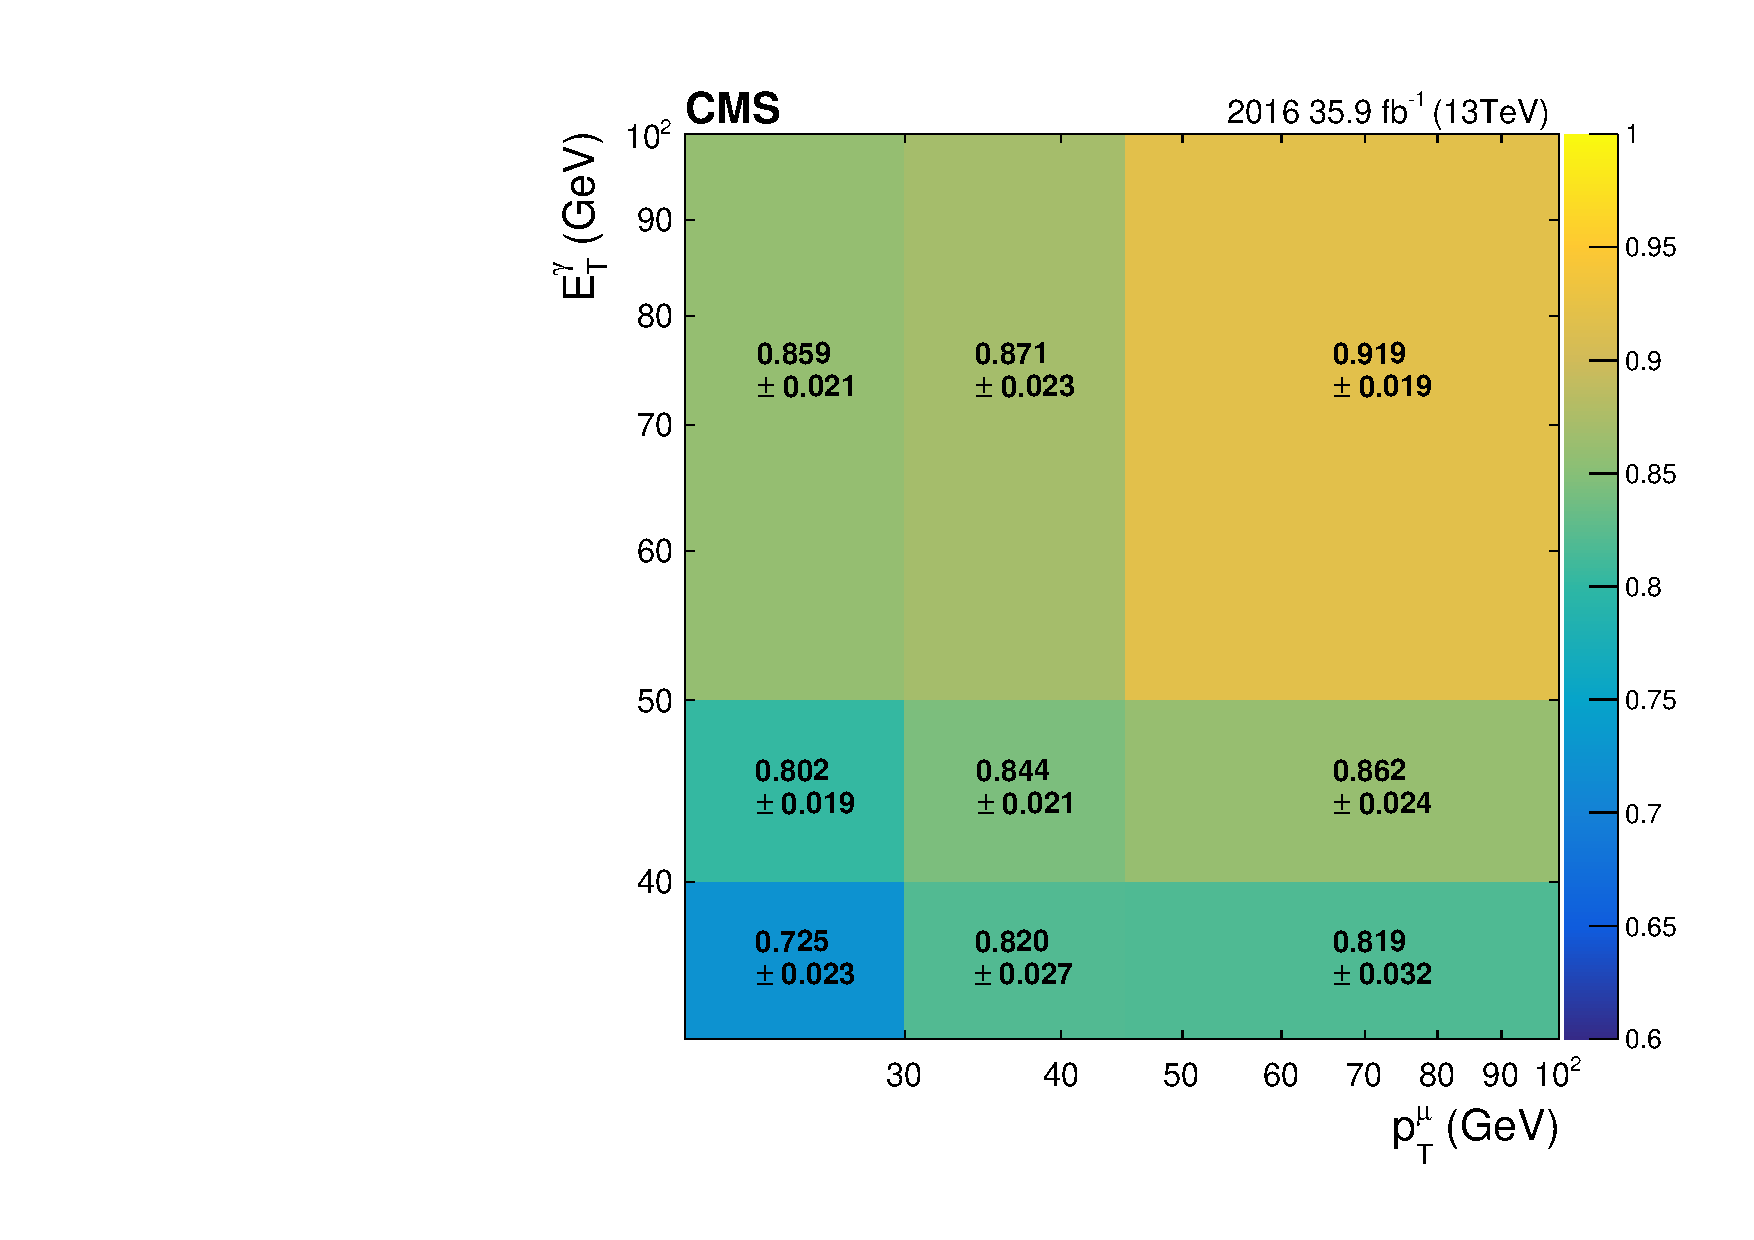
\includegraphics[width=0.47\textwidth]{Fig/Trigger/HZZID/Efficiency_MuPt_PhoEt_MC_DYJetsToLL_aMCatNLO_PU_nominal_EE}\\
		    \caption[Trigger Efficiency]{Trigger efficiency in bins of muon $\pt$ vs photon $\et$ for data with the photon in EB region (top left) and in EE region (top right), and for MC with the photon in EB region (bottom left) and in EE region (bottom right).}
		    \label{fig:TrigEffsep}
		\end{figure}
		
		\begin{figure}[p]
		        \centering
		    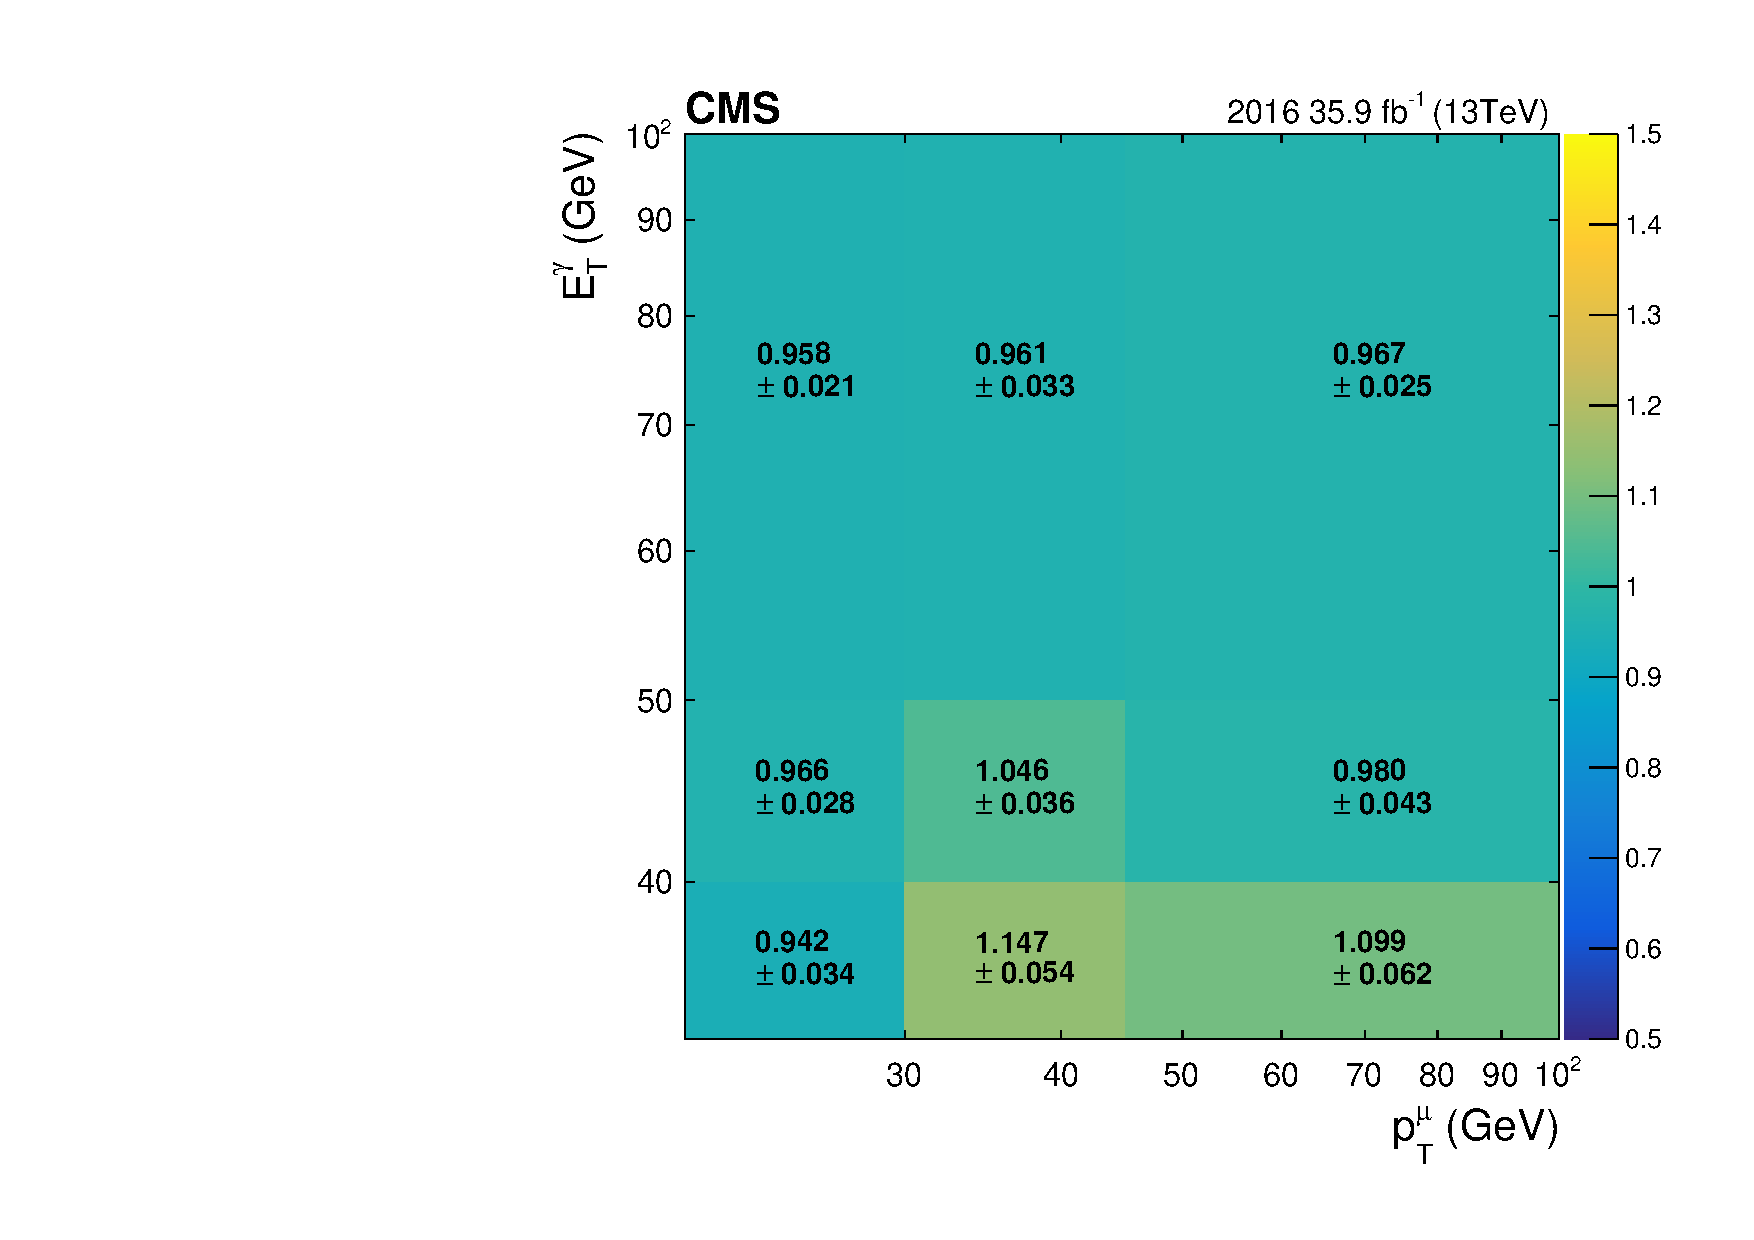
\includegraphics[width=0.47\textwidth]{Fig/Trigger/HZZID/TriggerEff_SFs_FinalVer_withSysUn_EB}~
		    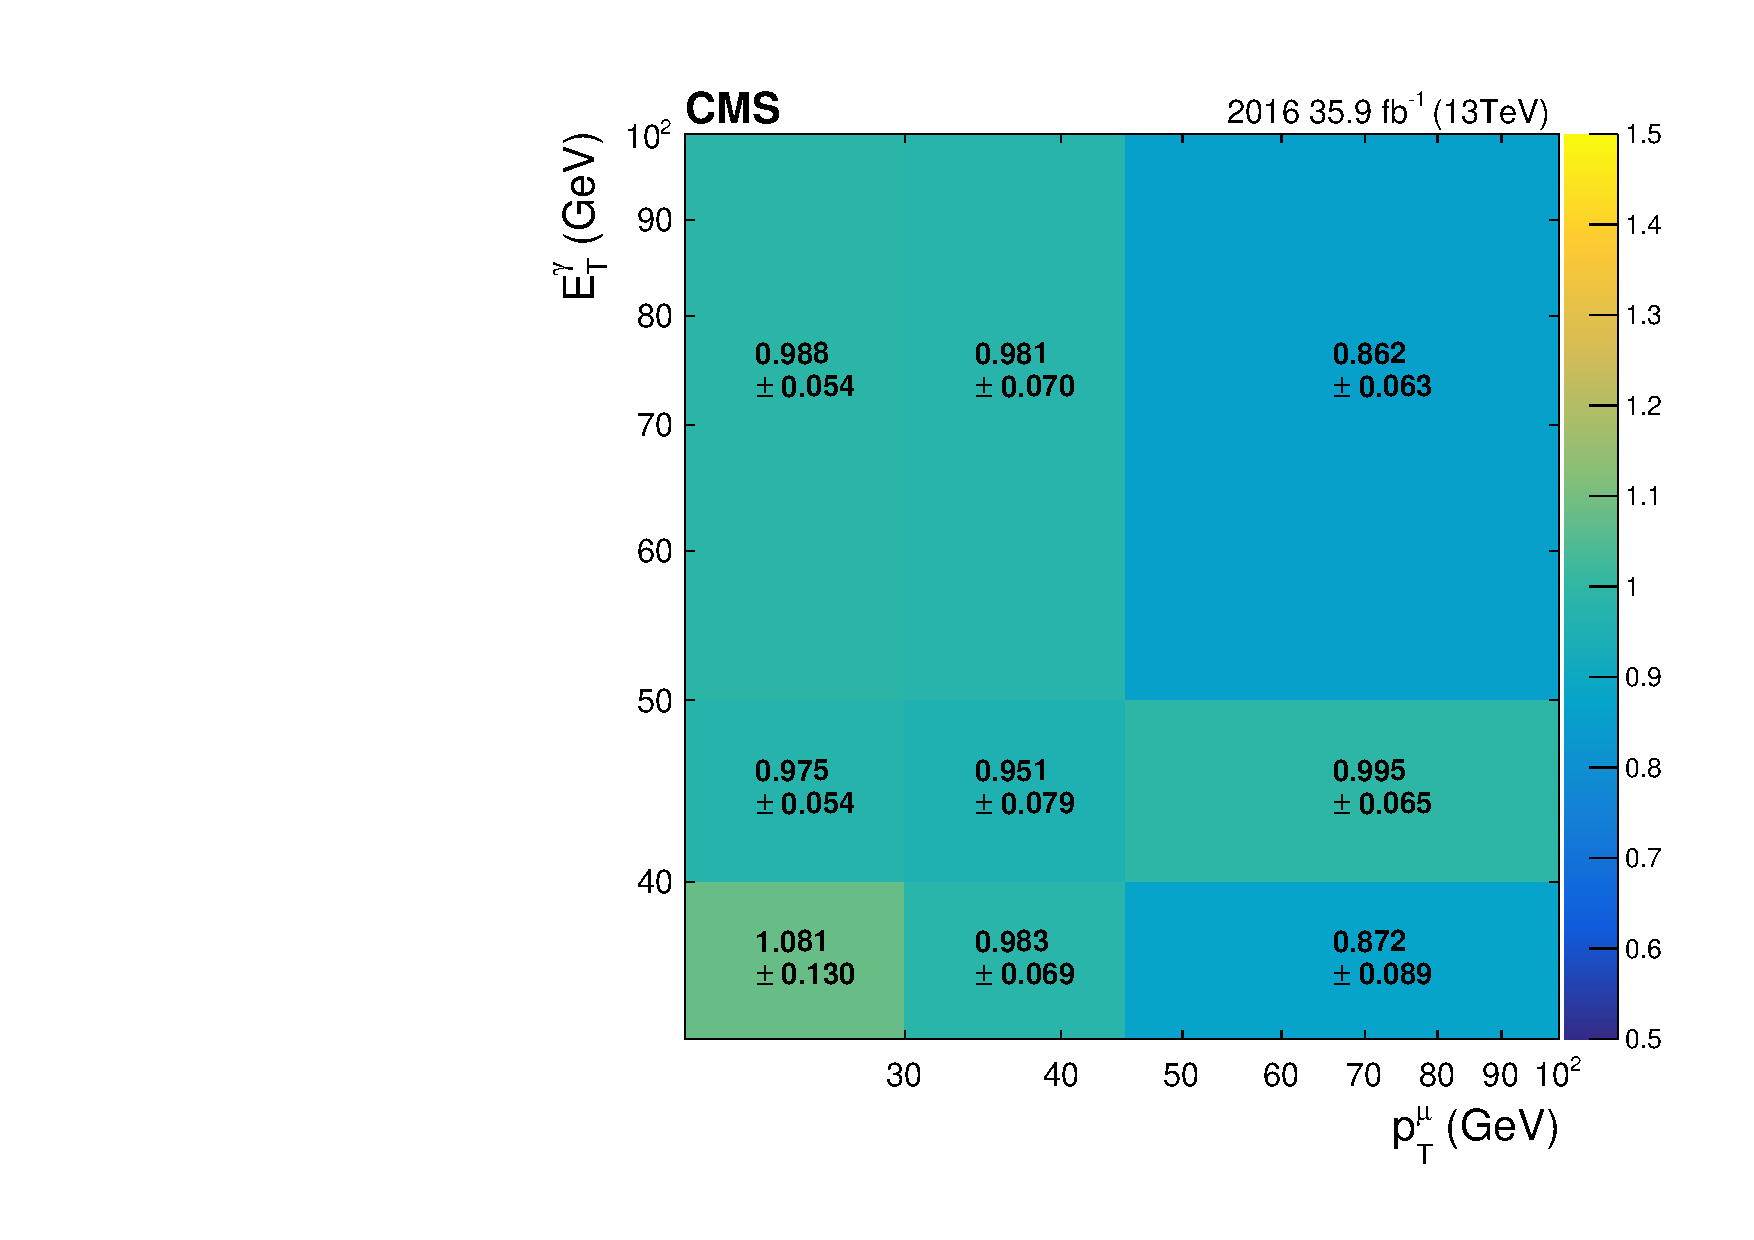
\includegraphics[width=0.47\textwidth]{Fig/Trigger/HZZID/TriggerEff_SFs_FinalVer_withSysUn_EE}\\
		    \caption[Trigger Efficiency Scale factor]{\label{fig:TrigEff}
		        Trigger efficiency scale factors in bins of photon $\pt$ vs muon $\pt$ for the selected photon in ECAL EB region (left), for the selected photon in ECAL EE region (right).}
		\end{figure}
	
	\clearpage
	
\section{Object identification}
	\subsection{Muon identification}
		\label{sec:muonid}
		It was observed in 2016 data that a single muon may be incorrectly reconstructed as two or more muons. To deal with this situation, the ``ghost cleaning'' procedure is performed. Tracker muons matched to segments in at least tow muons stations are retained. If there are two muons sharing more than 50\% of their segments, the one with lower reconstruction quality is removed.
	
		Two opposite-sign muons are selected with the identification requirements which are motivated by $\PH\to\cPZ\cPZ^{*}\to 4\ell$ analysis~\cite{Sirunyan:2017exp} and are listed as follows: 
		\begin{itemize}
		\item Muons must be reconstructed as particle-flow muons, and can either be global muons or tracker muons. Those only reconstructed as standalone muon are rejected.
		\item $\pt > 4$, $|\eta| < 2.4$
		\item Muons must have $d_{xy}< 0.5\unit{cm}$, $d_{z} < 1\unit{cm}$, where $d_{xy}$ and $d_{z}$ are defined as the closest distance between the track of the muon and the PV in the $\phi$ plane and the z direction respectively. 
		\item Significance of the impact parameter in 3-dimensional space ${\rm SIP_{3D}}=|IP/\sigma_{IP}| < 4$, where IP is the closest distance between the track of the muon and the event vertex, $\sigma_{IP}$ is the uncertainty of the IP. 
		\end{itemize}
		The usage of impact parameter cuts suppresses the muons from the decays of heavy-flavor hadrons or products of cosmic ray. If the muon $\pt$ is greater than 200\GeV, it is selected if it passes Tracker High-$\pt$ ID. After the whole set of selection, there is no event with the muon $\pt$ greater than 200\GeV in both Higgs and $\cPZ$ boson searches.
%		\begin{itemize}
%		\item Muons must match to segments in at least two muon stations.
%		\item Good $\pt$ measurement. $\frac{\pt}{\sigma_{\pt}} < 0.3$.
%		\item Muons must have $d_{xy}< 0.2\unit{cm}$, $d_{z} < 0.5\unit{cm}$.
%		\item Muons have at least one pixel hit in order to suppress muons from in-flight decays.
%		\end{itemize} 

		In order to discriminate prompt muons from Higgs ($\cPZ$) boson decays from those from electroweak decays of hadrons within jets, the Particle-Flow isolation requirement is applied. In this analysis, the relative isolation is calculated for the leading muon.
	
		\begin{equation}
		\mathcal{I}^{\mu}\equiv \frac{\sum \pt^{\text{charged}} + \max \bigg [0, \sum \et^{\text{neutral}} + \sum \et^{\gamma} - \pt^{\text{PU}}(\mu)\bigg ]}{\pt^{\mu}}
		\end{equation}	
		
		A cone of size $\Delta R = \sqrt{(\Delta \eta)^2 +(\Delta \phi)^2} = 0.3$ is constructed around the direction of muon momentum. The $\sum \pt^{\text{charged}}$ is the scalar sum of the transverse momenta of charged hadrons originating from the chosen primary vertex of the event. The $\sum \et^{\text{neutral}}$ and $\sum \et^{\gamma} $ are the scalar sums of the transverse energy for neutral hadrons and photons, respectively. Since the isolation variable is sensitive to energy deposits from pileup interactions, the $\pt^{\text{PU}}(\mu)$ contribution is subtracted. The pileup contribution $\pt^{\text{PU}}(\mu) \equiv 0.5 \sum_{i} \pt^{\text{PU}, i}$, where $i$ runs over the momenta of the charged hadron PF candidates not originating from the primary vertex, and the factor of 0.5 corrects for the different fraction of charged and neutral particles in the cone. 
		These momentum and energy sums do not include the contribution from the muon itself. $\Delta\beta$ correction is applied, where $\Delta\beta \equiv 0.5 \sum^{\text{charged\ hadron}}_{PU} \pt$ is the estimation of the energy deposit of neutral hadrons and photons from other pileup vertices. The isolation is required to be less than 0.35 for the leading muon, corresponding to $\sim 96\%$ of signal efficiency and $\sim 81\%$ of background rejection power. 
		
		The reason that the isolation is not calculated for the trailing muon is that the $\Delta R$ for most of selected muon pairs are less than 0.3 (as can be seen from Fig.~\ref{fig:dist-4},~\ref{fig:dist-5}, and~\ref{fig:dist-6}), which means that the trailing muon is within the isolation cone defined with the leading muon.  
		The Isolation efficiencies as functions of $\pt^{\text{leading}\ \mu}$, $\pt^{\text{trailing}\ \mu}$, $\eta^{\text{leading}\ \mu}$, $\eta^{\text{trailing}\ \mu}$, and $\pt^{\mu\mu}$ are shown in Fig.~\ref{fig:IsoEff}. Applying isolation on both muons is about 7\% less efficient than applying it only on the leading muon, which is due to the fact that the trailing muon $\pt$ is not significantly greater than other activities in the defined cone.	 
		
		\begin{figure}[p]
		  \centering
		  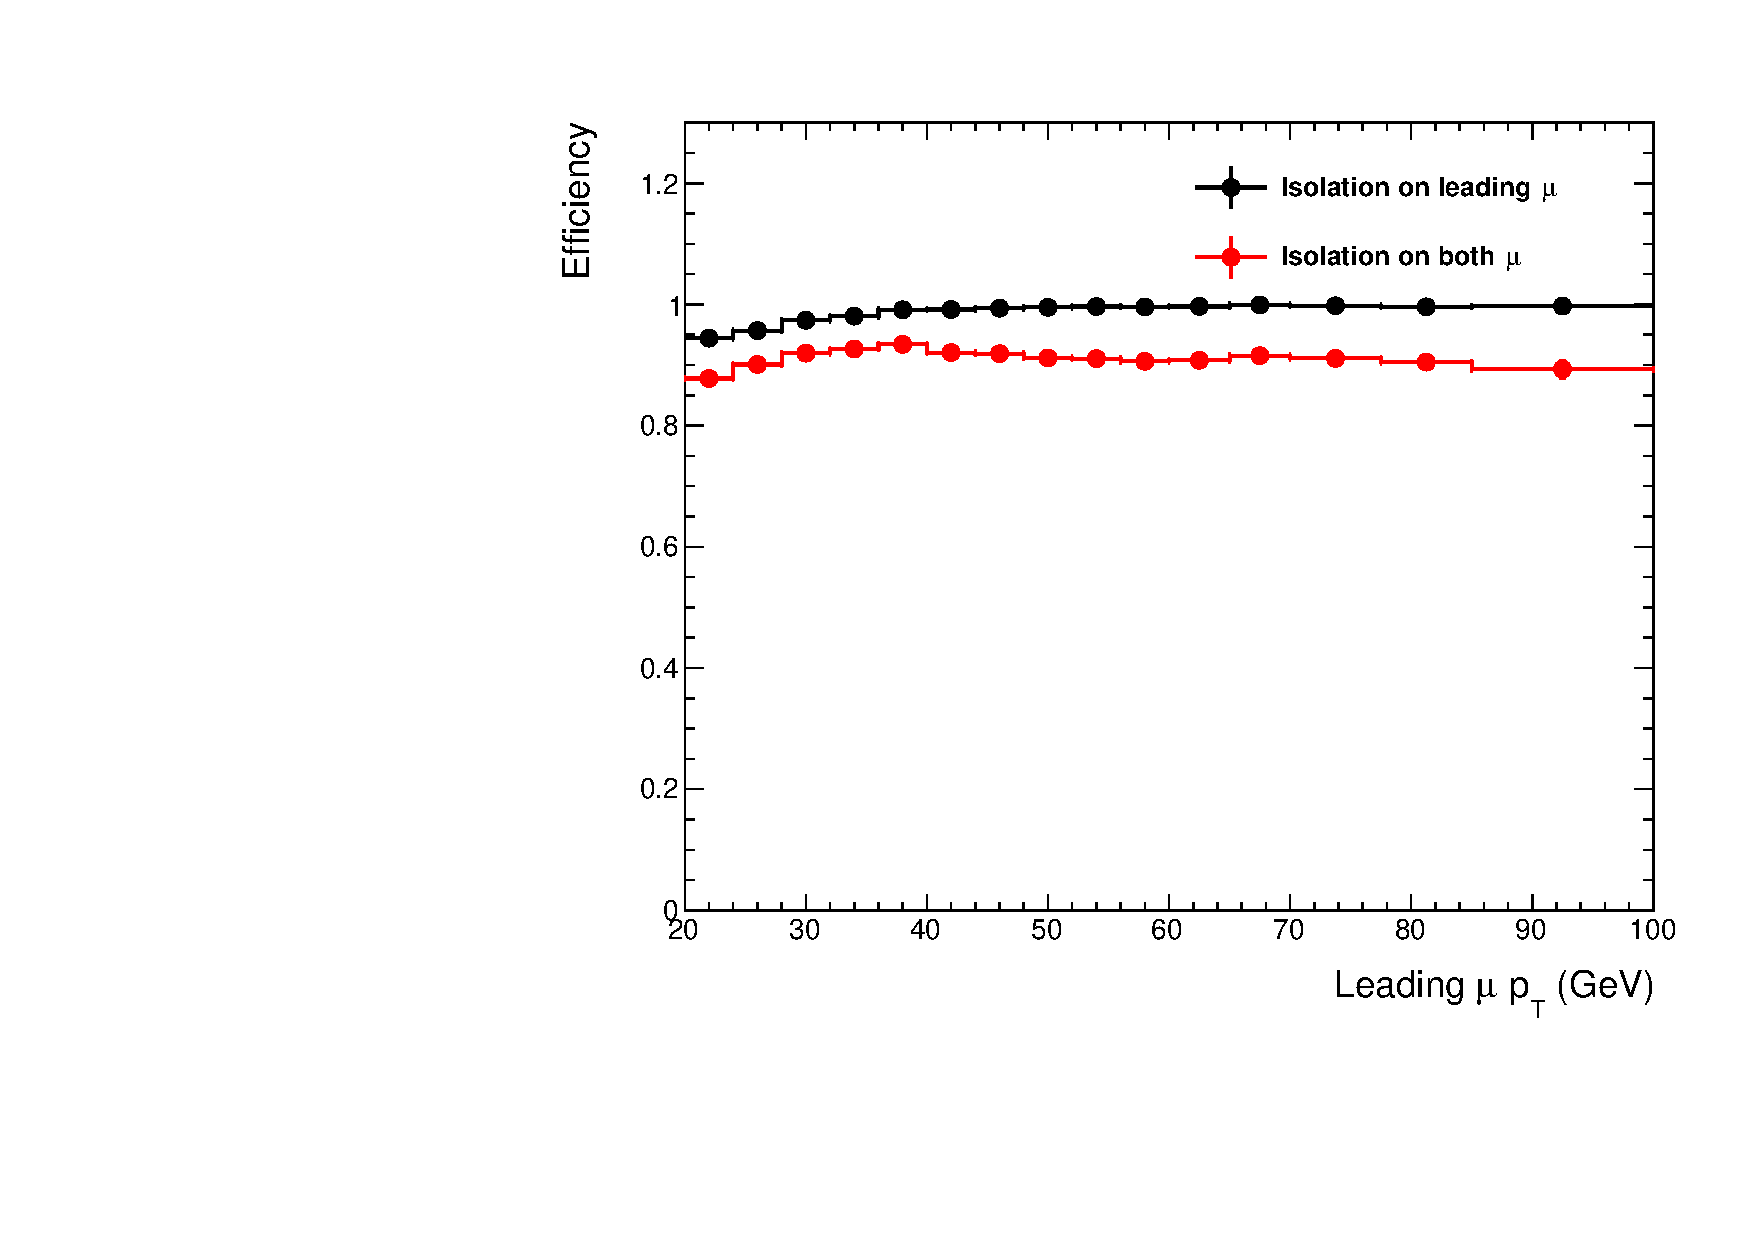
\includegraphics[width=0.5\textwidth]{Fig/EffIso/EffIso_LeadMuPt}~
		  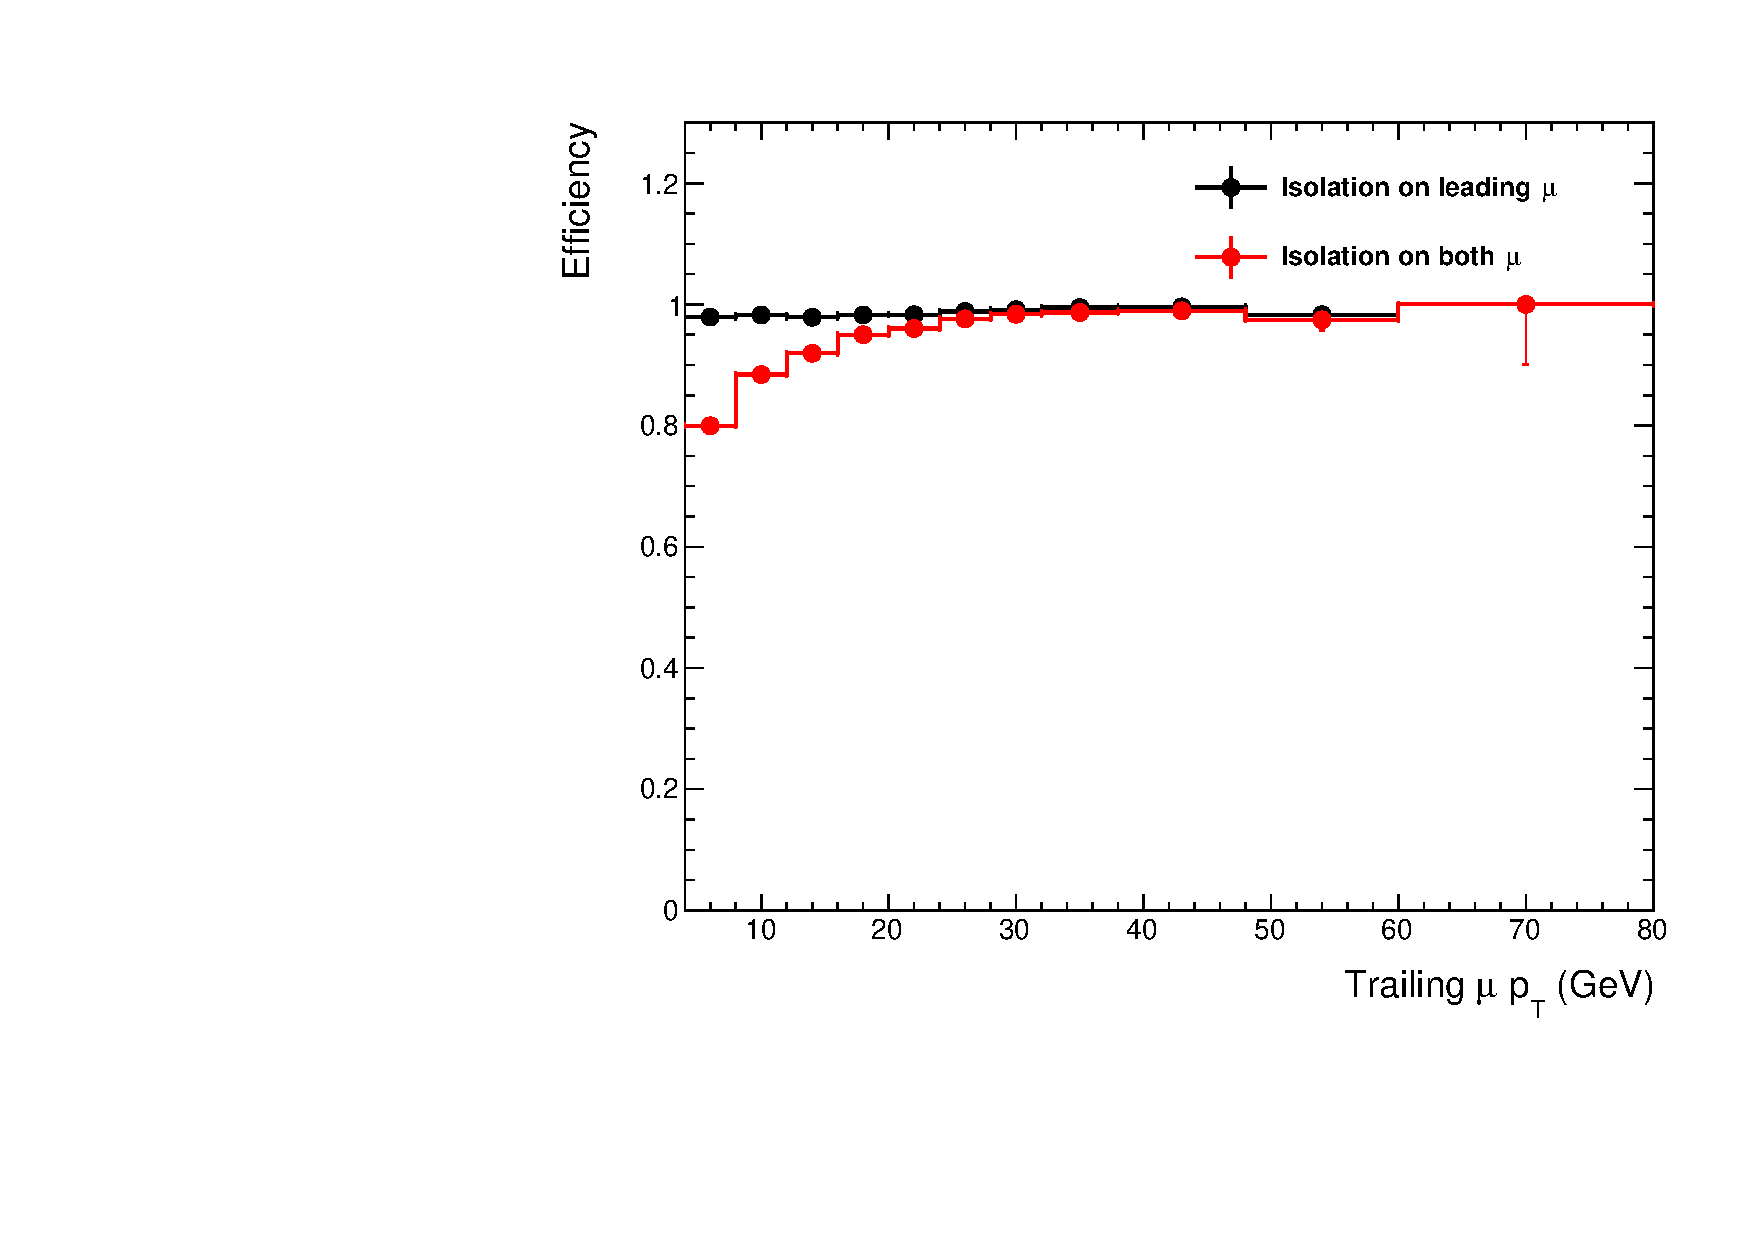
\includegraphics[width=0.5\textwidth]{Fig/EffIso/Eff_Iso_TrailMuPt}\\
		  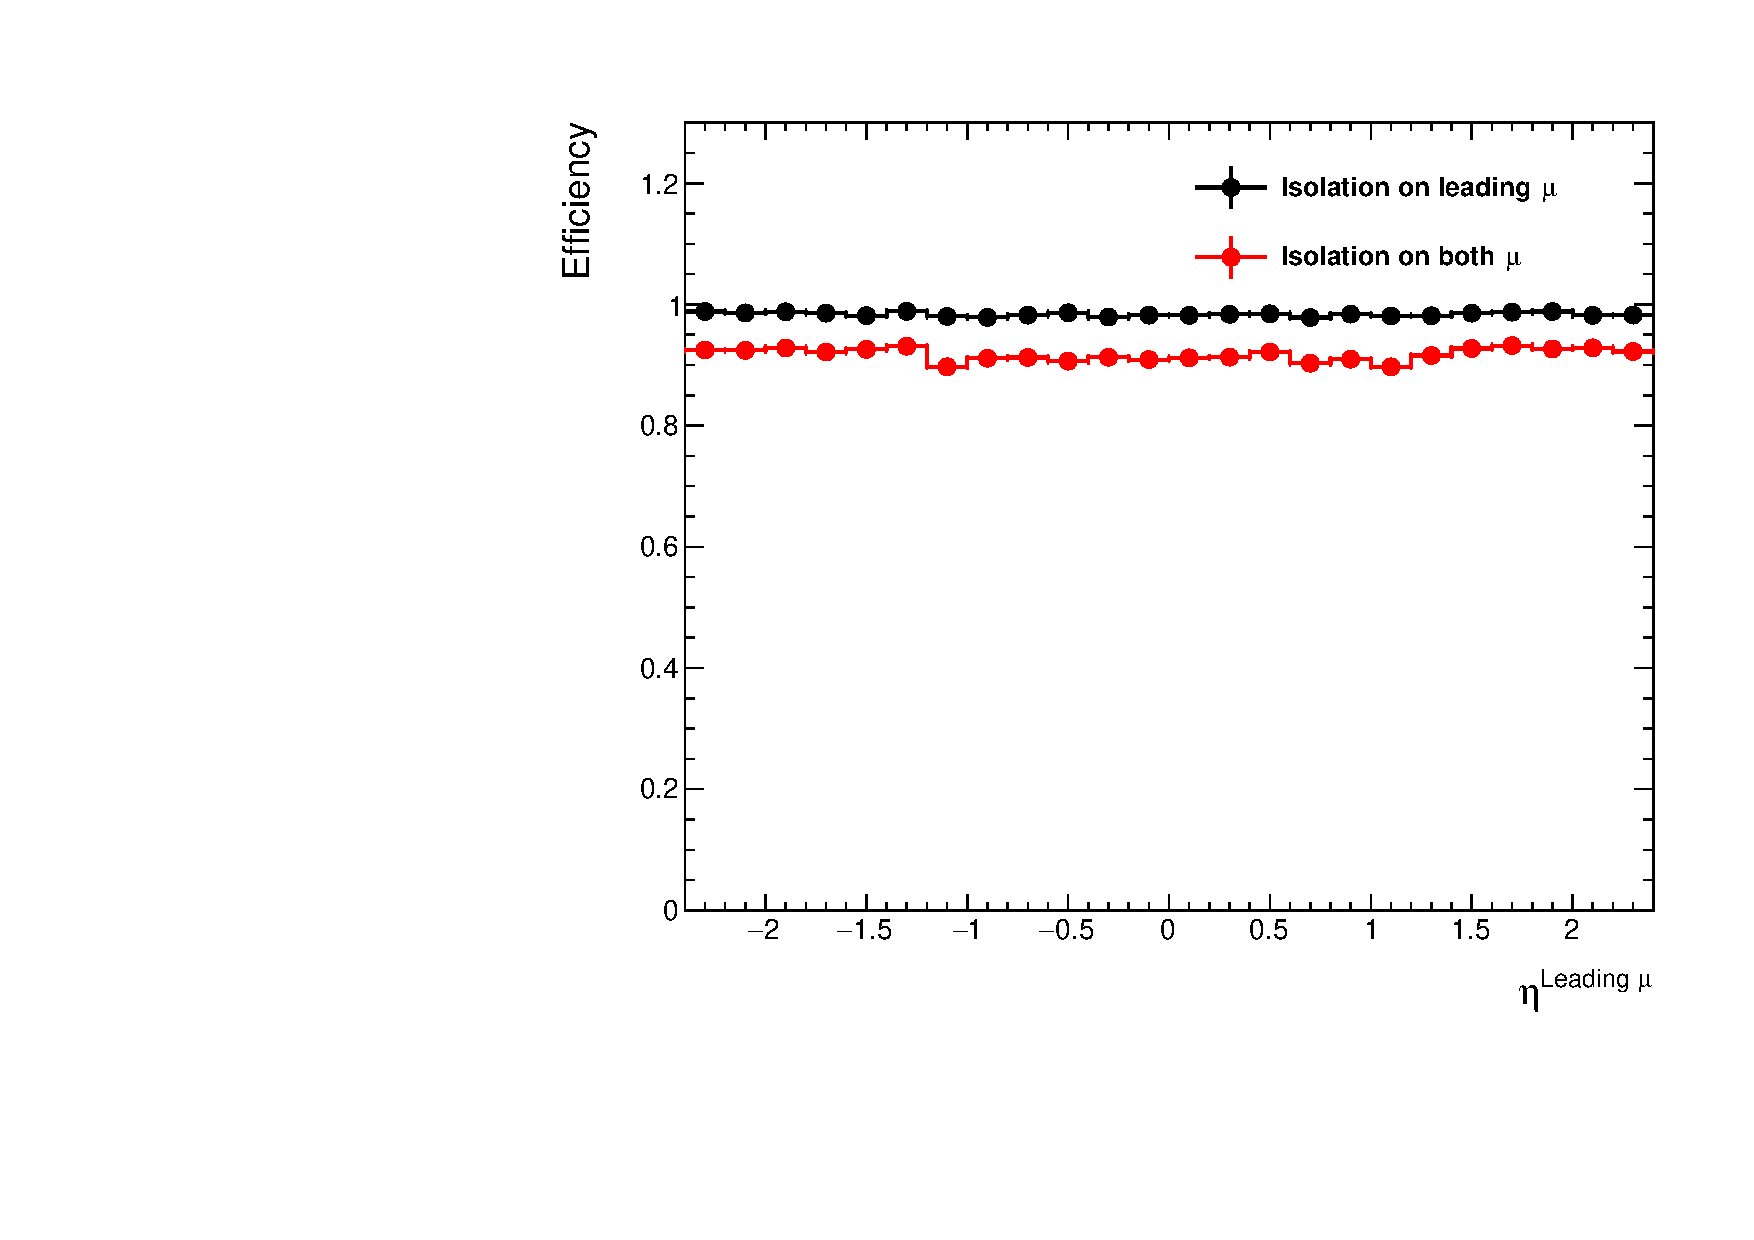
\includegraphics[width=0.5\textwidth]{Fig/EffIso/EffIso_LeadMuEta}~
		  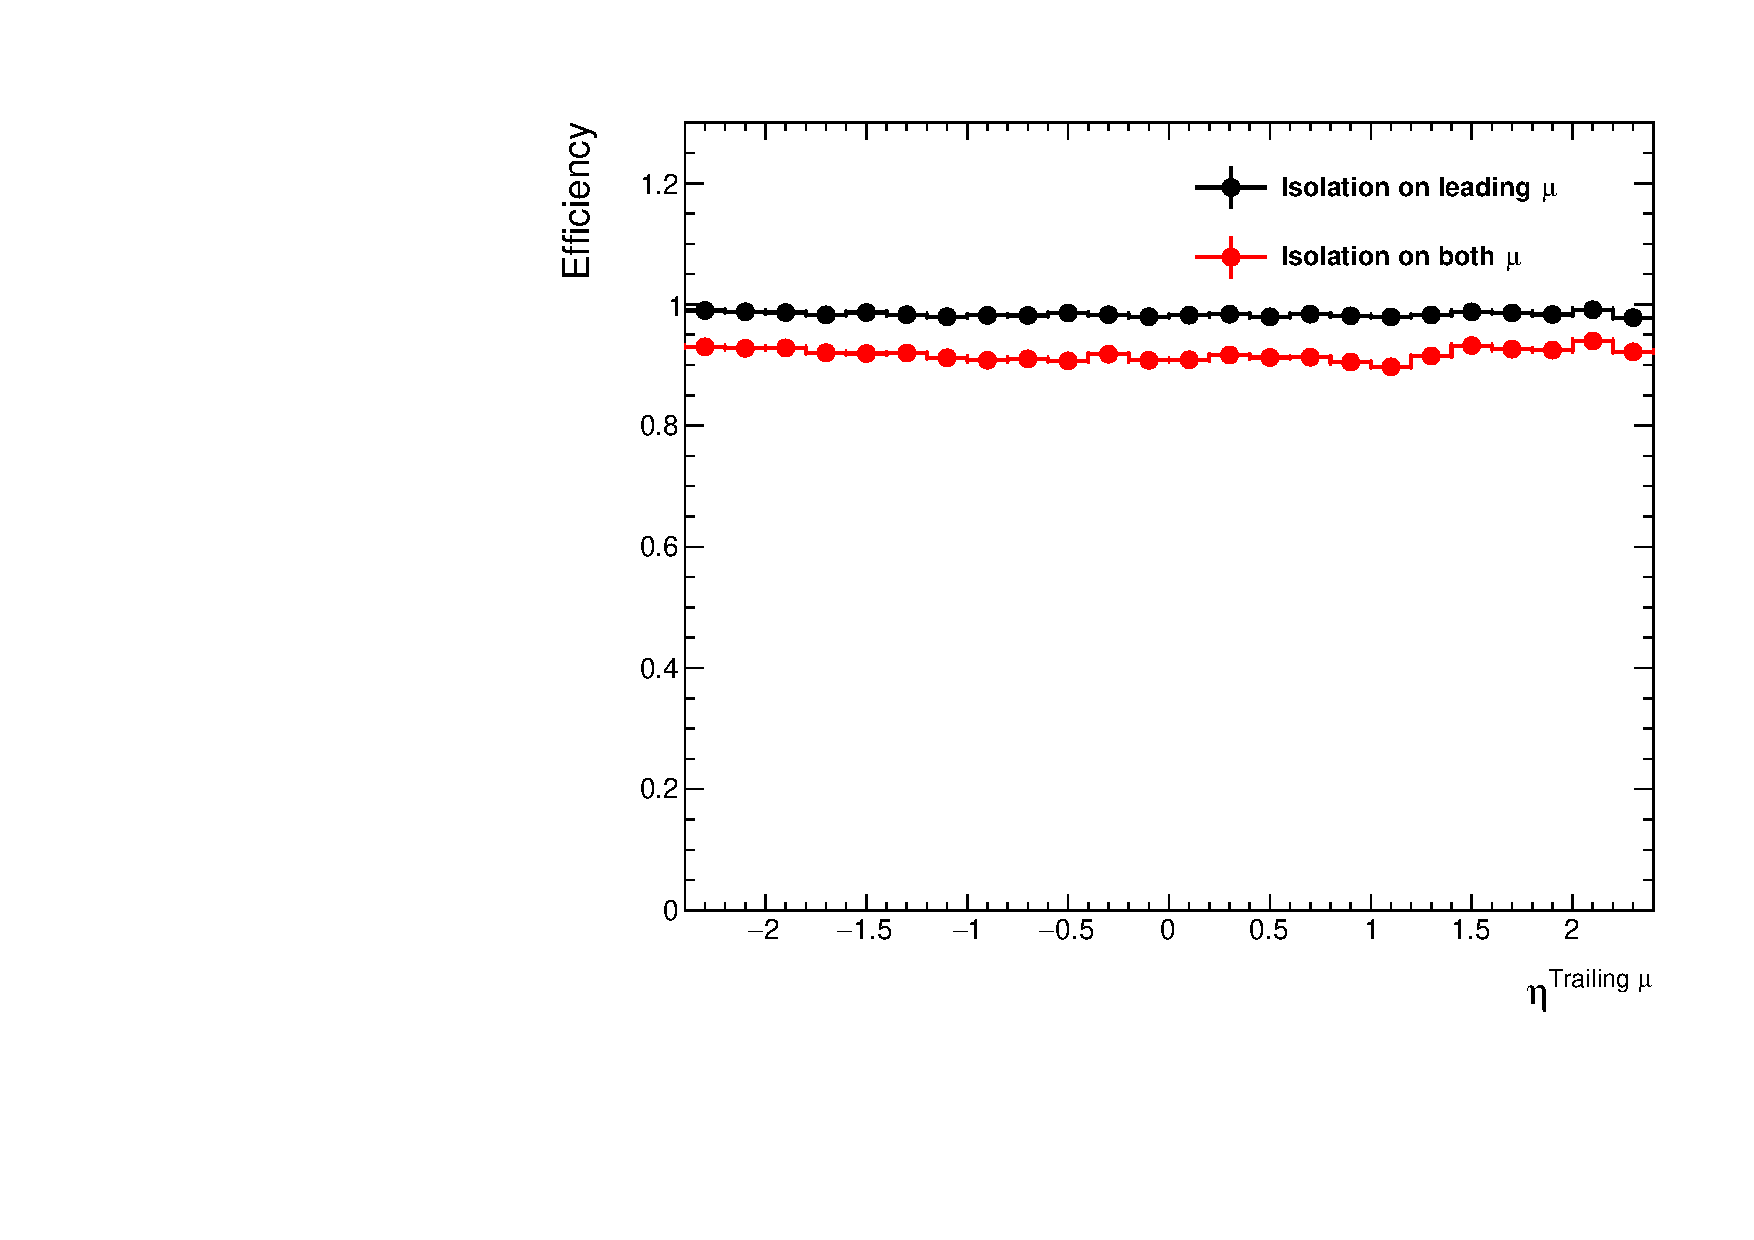
\includegraphics[width=0.5\textwidth]{Fig/EffIso/EffIso_TrailMuEta}\\
		  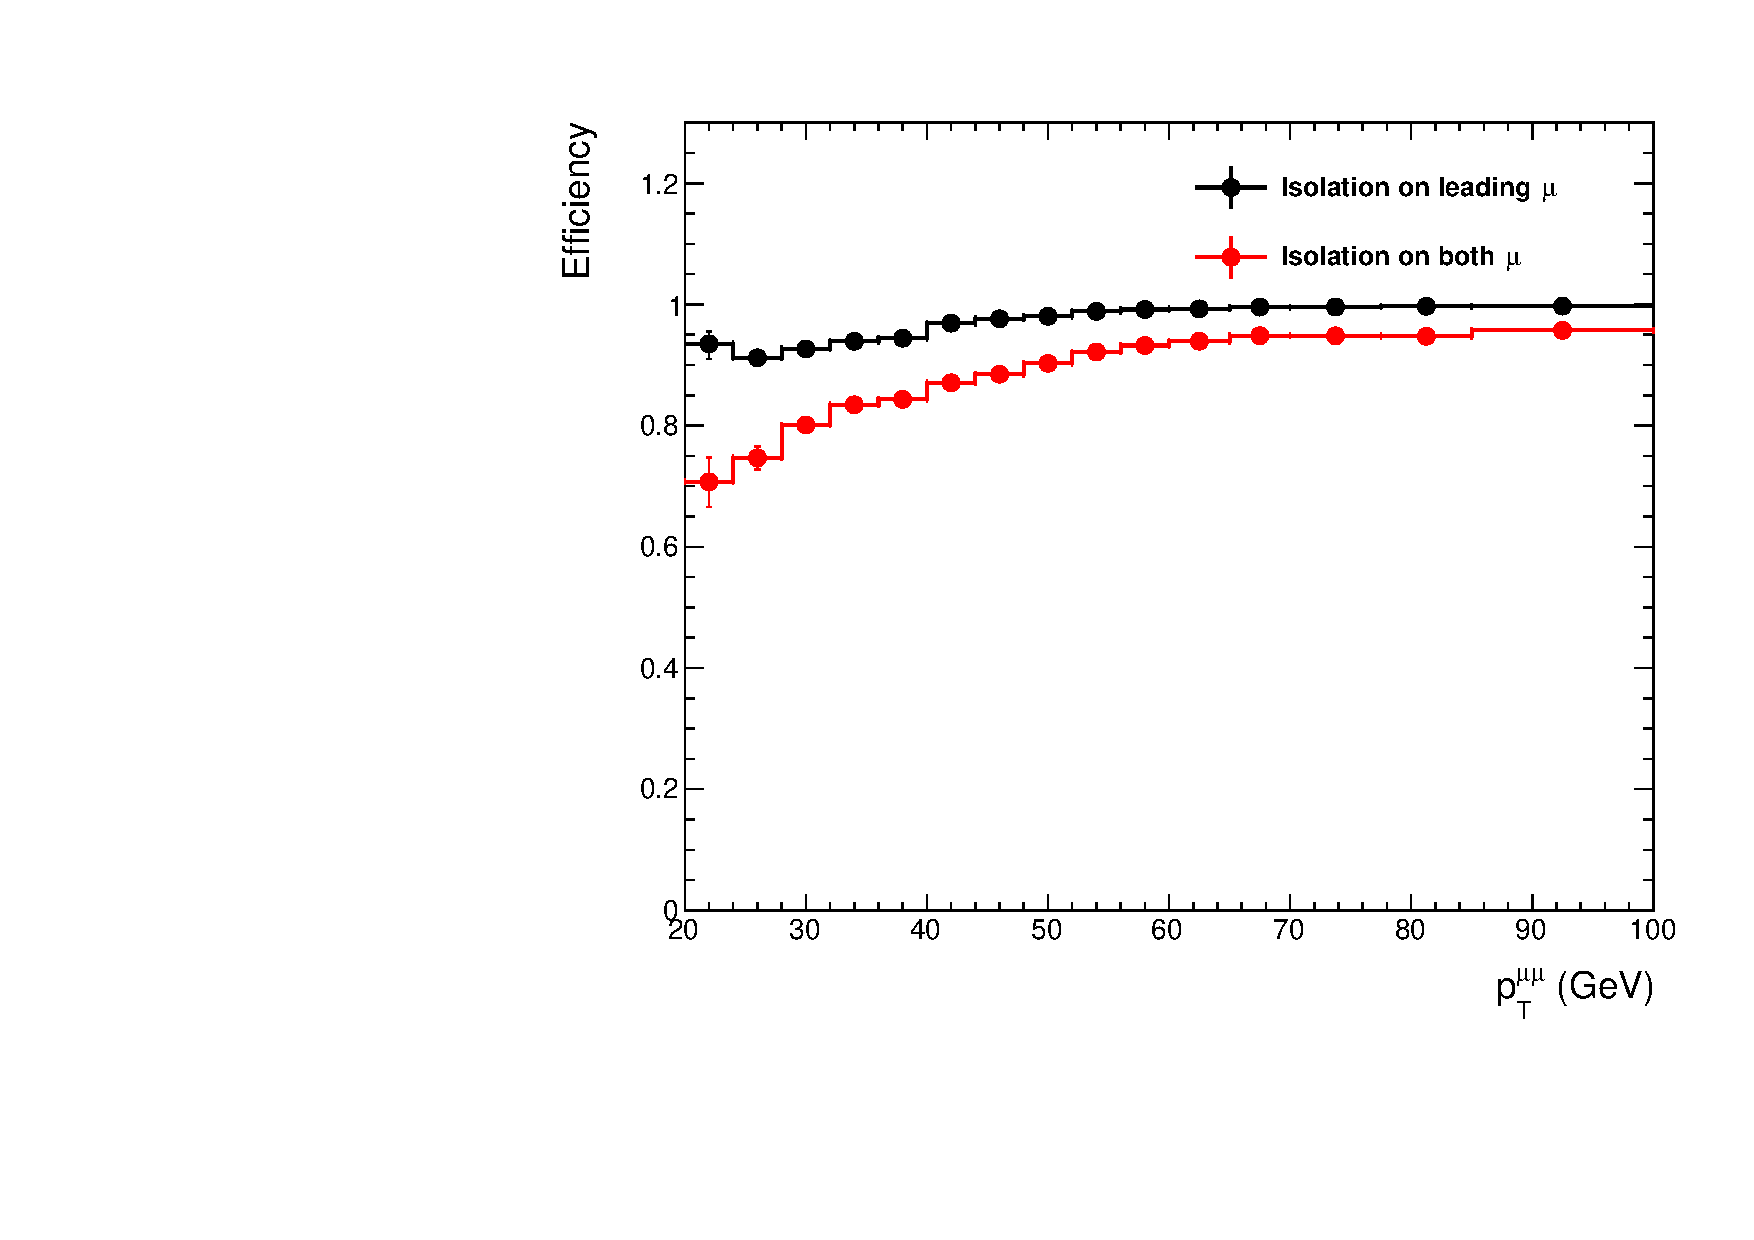
\includegraphics[width=0.5\textwidth]{Fig/EffIso/EffIso_DimuPt}\\
		  \caption{Relative isolation efficiency for muon as function of $\pt^{\text{leading}\ \mu}$ (top left), $\pt^{\text{trailing}\ \mu}$ (top right), $\eta^{\text{leading}\ \mu}$ (bottom left), $\pt^{\mu\mu}$ (bottom right).\label{fig:IsoEff}}
		\end{figure}	
		
		When the subleading muon is in the isolation cone of the leading muon, its $\pt$ contribution is subtracted in the isolation sum of the leading muon, and vice versa. This can be verified by looking at the isolation of the leading muon divided by the $\pt$ of the trailing muon in each sample with isolation requirement relaxed, as shown in Fig.~\ref{fig:IsoCheck}. All the distributions are normalized to unity. If the subleading muon is not excluded in the isolation of the leading muon, then it is expected that there will be a peak at $\sim 1$ on the distribution, which is not seen. 
		
		\begin{figure}[!ht]
		  \centering
		  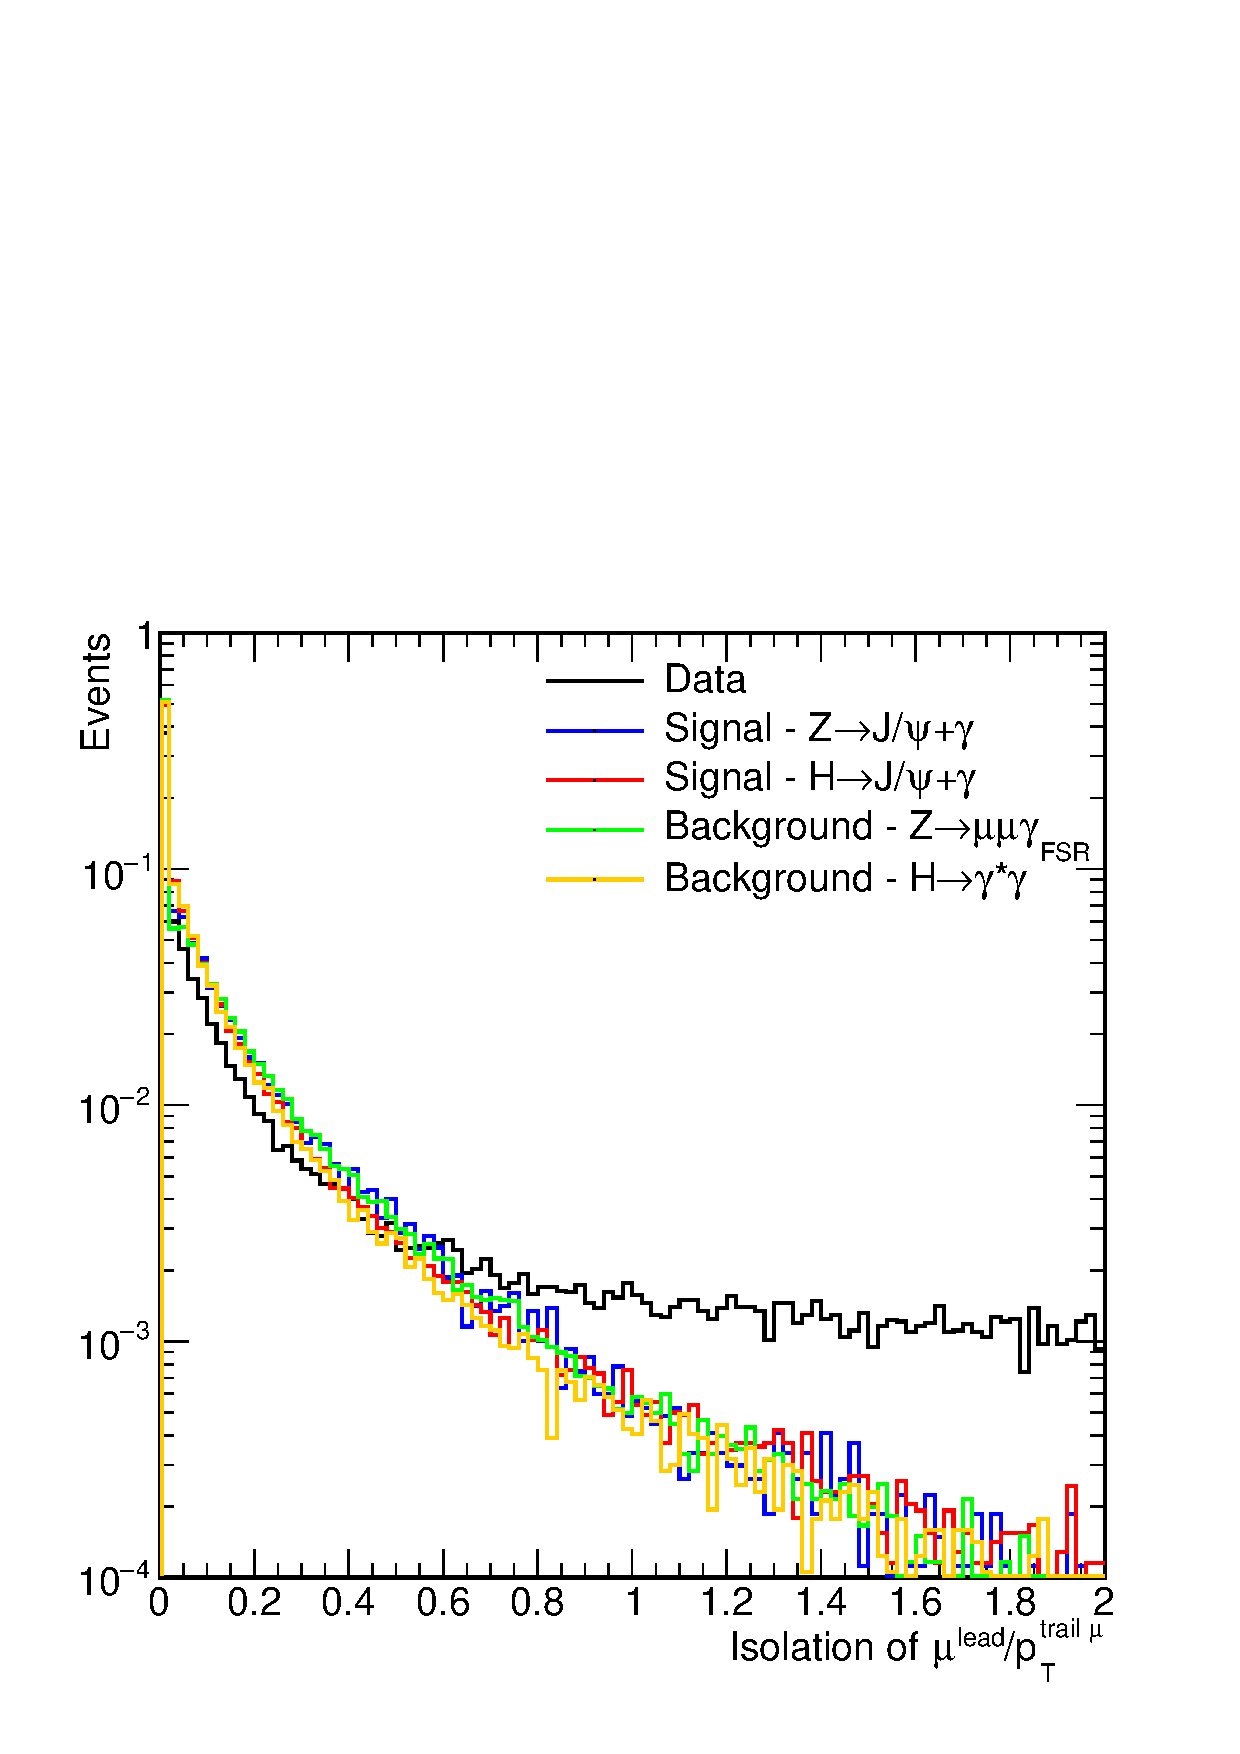
\includegraphics[width=0.5\textwidth]{Fig/Mu1Iso_div_mu2Pt_All}\\
		  \caption{The isolation of the leading muon divided by the $\pt$ of the trailing muon in each sample. All the distributions are normalized to unity.\label{fig:IsoCheck}}
		\end{figure}
		
		Fig.~\ref{fig:FakeMuEst} shows the $m_{\mu\mu}$ distributions of the events selected with isolation requirement (left) and without isolation requirement (right). Muons from $\JPsi$ decay must be true muons, so the fake muons should mostly fall in the continuum background but not form in $\JPsi$ peak. Therefore, the numbers of background, Nbkg, from the fit can roughly tell us how many fake muons will be selected if no isolation requirement is imposed. By removing the isolation cut, Nbkg changes from $\sim 492$ to $\sim 756$, meaning that fake muons roughly decrease by 34.9\%. 
		
	\begin{figure}[!ht]
		  \centering
		  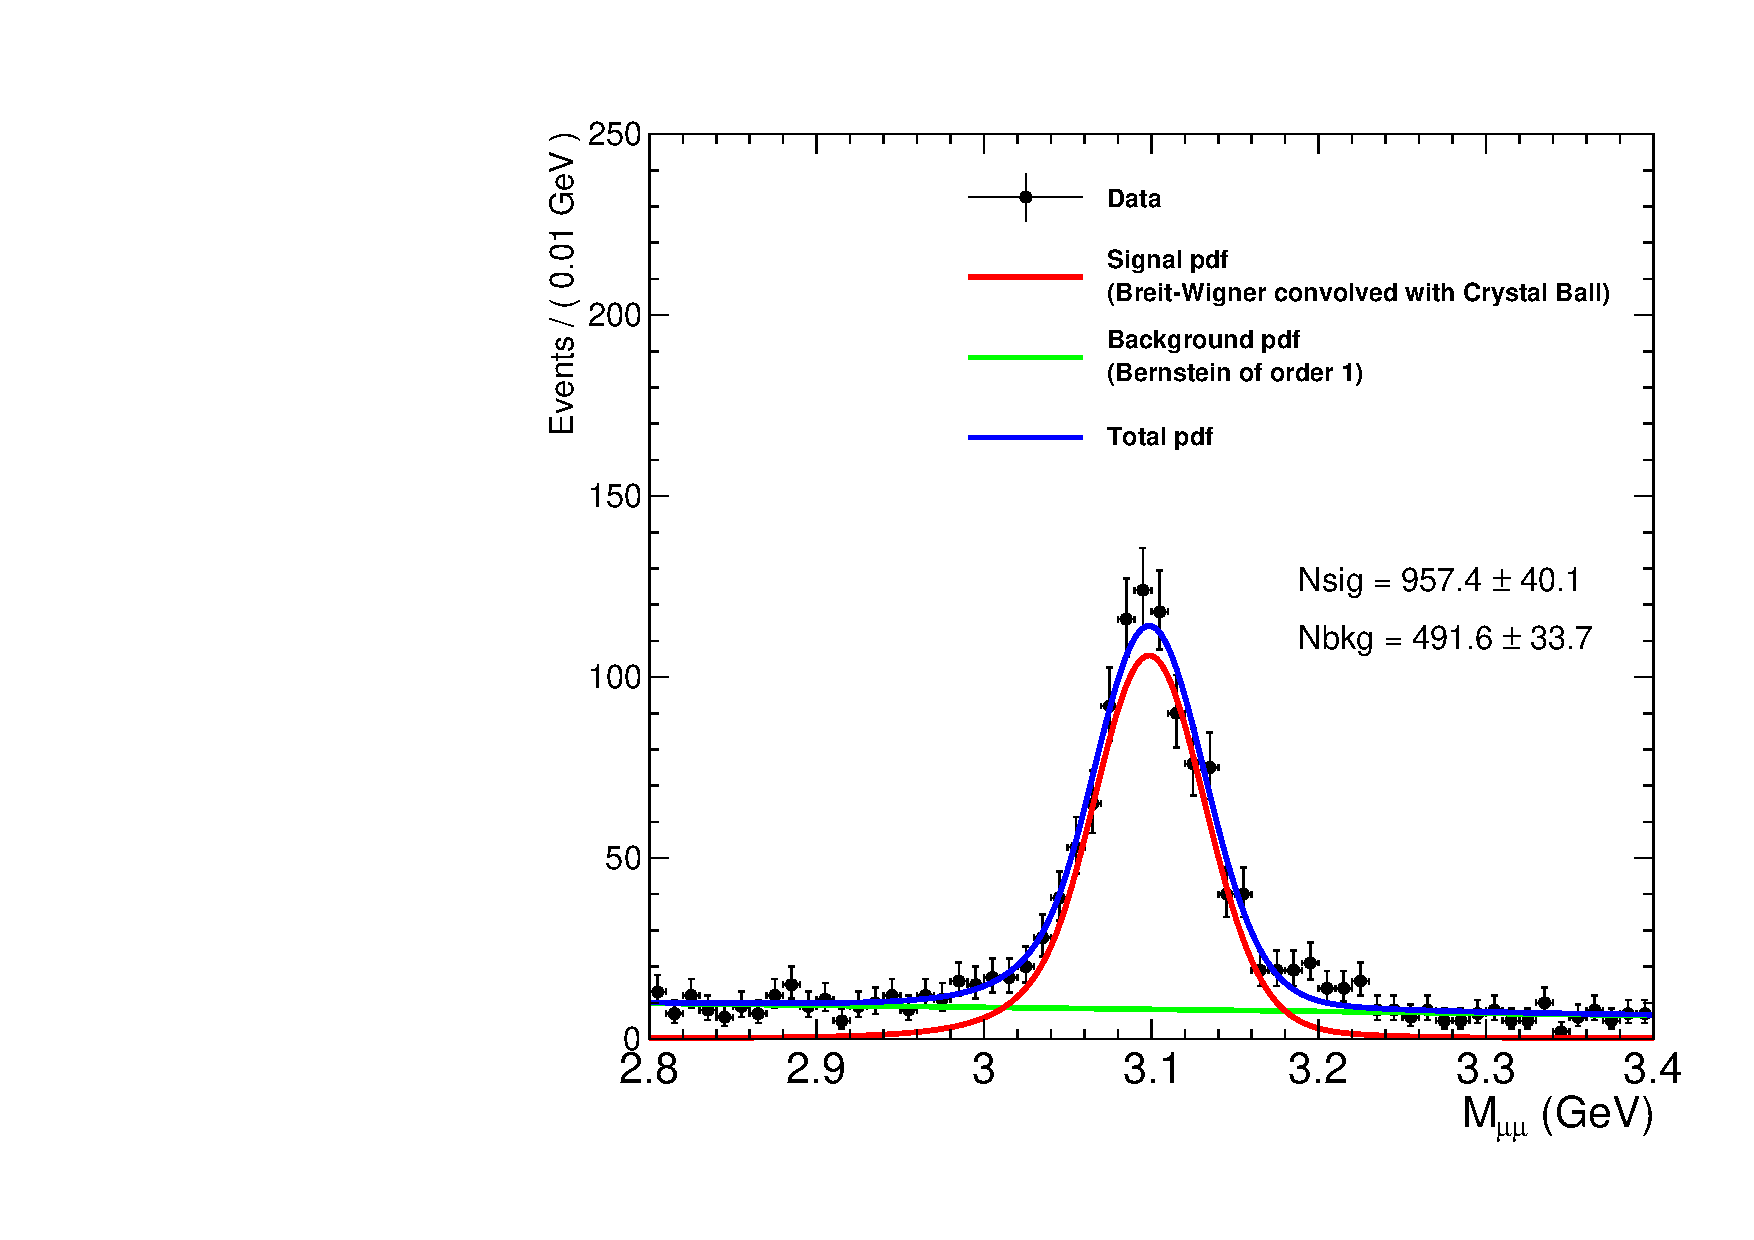
\includegraphics[width=0.5\textwidth]{Fig/FakeMuEst/Dimuon_Nominal}~
		  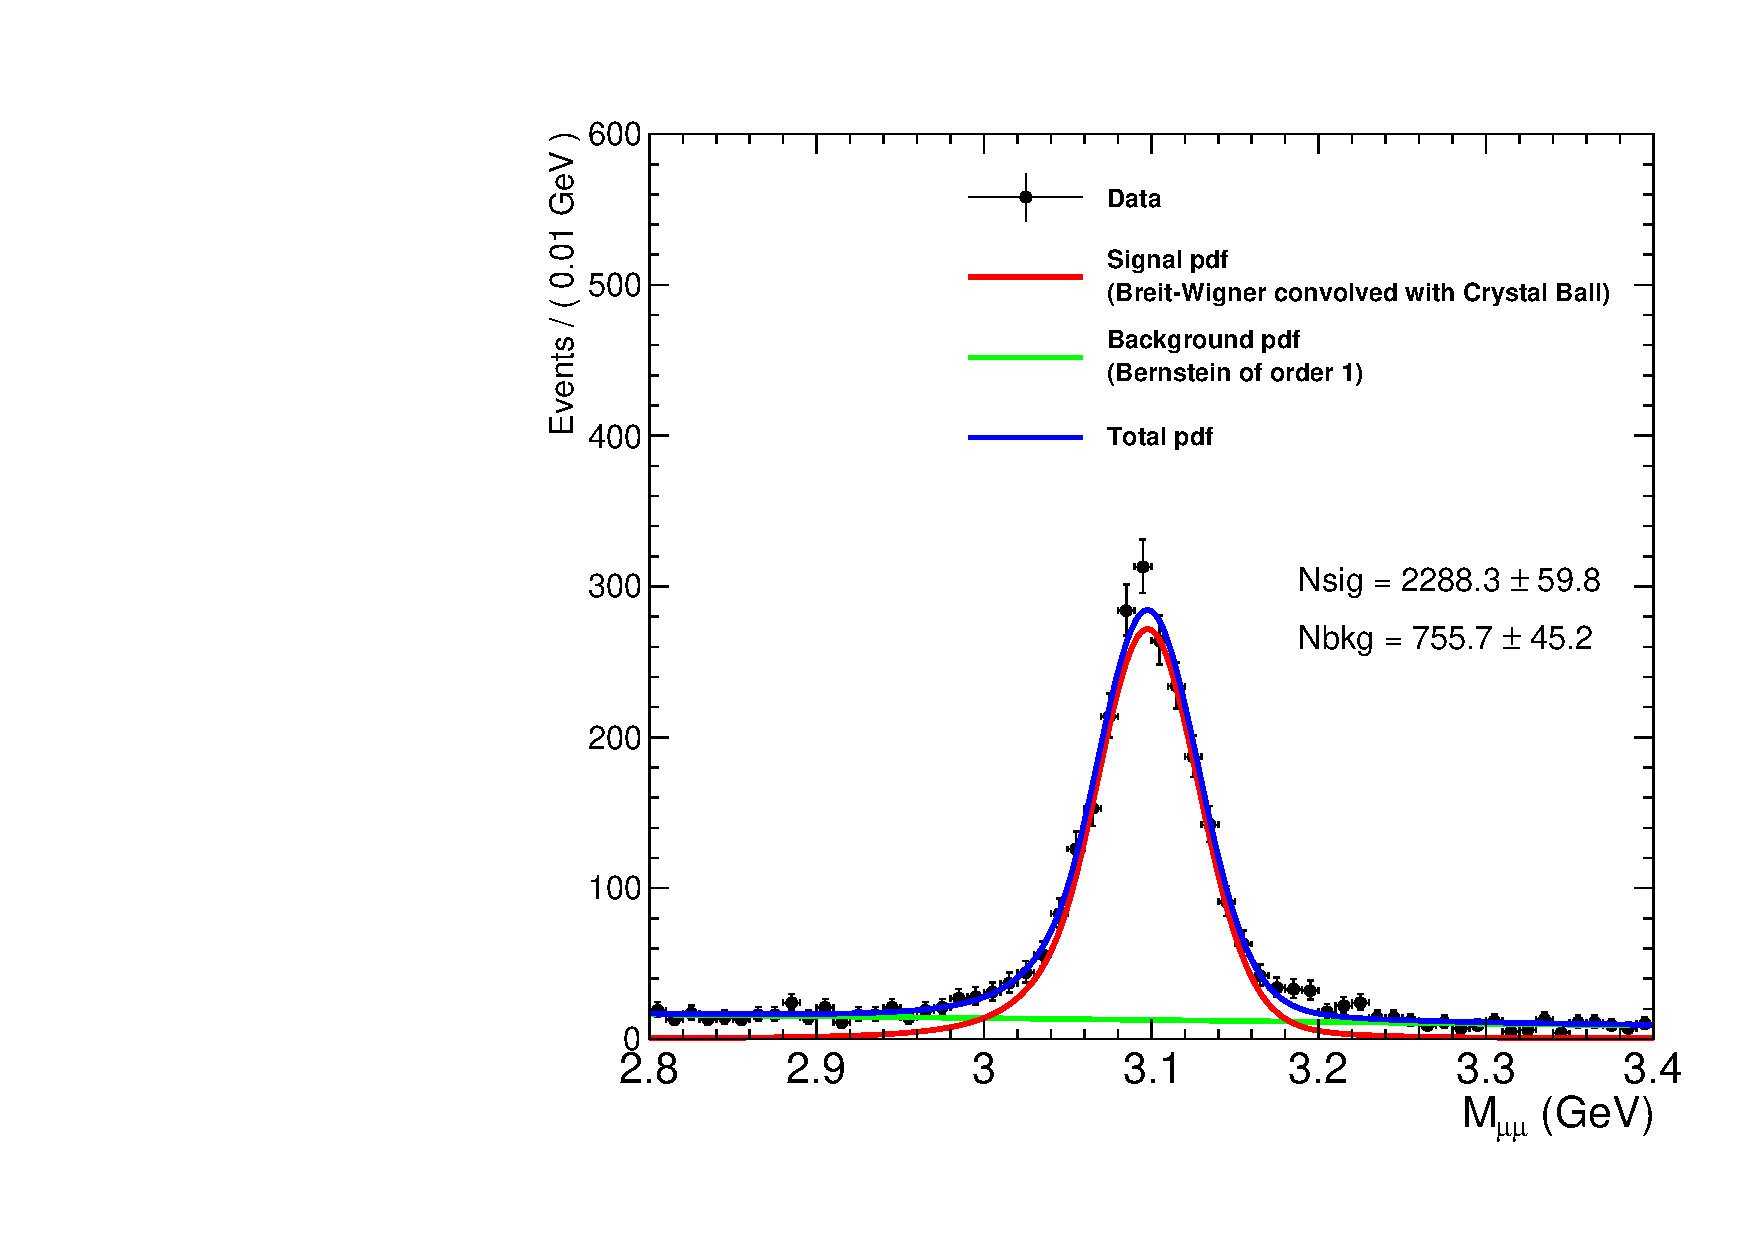
\includegraphics[width=0.5\textwidth]{Fig/FakeMuEst/Dimuon_NoIso}\\
		  \caption{The $m_{\mu\mu}$ distributions of the events selected with isolation requirement (left) and without isolation requirement (right). By removing the isolation cut, the fake muons roughly decrease by 34.9\%.}
		  \label{fig:FakeMuEst}
		\end{figure}	
		
		The other information that can be extracted here is that, lots of events from QCD background can be removed by applying the isolation, based on the fact that the $\JPsi$ in the distributions are from QCD events rather than from actual signal $\PH (\cPZ)\to(\JPsi)\gamma$. Whether the isolation is applied or not has negligible impact on the expected signal yields (less than 1\%).
		
		\subsubsection{Muon momentum calibration}
		In this analysis, Rochester Muon Momentum Corrections~\cite{Bodek:2012id} derived for 2016 dataset are applied.
		Biases in the measurement of muon momenta in hadron collider experiments can originate from several sources such as misalignment of the detectors, the deficiency in the software reconstruction, and uncertainties in magnetic field. Corrections are developed to remove such biases. The momentum scale corrections are extracted using the average of $1/\pt \ (<1/\pt>)$ spectra of muons from $\cPZ$ decay, while the resolution corrections and scale factors are derived by comparing the $m_{\mu\mu}$ distributions between data and MC. The corrections are then applied to correct the momentum scale in data events and resolution in simulated events. 
		%The corrections were derived from combined datasets. No significant Run-dependence of correction was observed when the corrections were applied to different Runs. \\ 
		We validate whether the Rochester correction would give consistent energy scale and resolution between data and MC for the muons from decay of $\JPsi$ candidates in $\PH\to(\JPsi)\gamma$ events. In this validation study, the events are required to satisfy the nominal selection requirements with relaxed dimuon and photon transverse momenta ($\pt^{\mu\mu}, \et^{\gamma}/m_{\mu\mu\gamma} > 0.16(20/125)$). To quantify the scale and resolution, a Breit-Wigner convolved with a Crystal Ball function (Eq.~\ref{eqn:f_MC}) is used to fit the distribution for the signal events. For the data events, Breit-Wigner convolved with a Crystal Ball function in addition of the Bernstein $1_{\text{st}}$ polynomial (Eq.~\ref{eqn:f_data}) is used as model. As can be seen in Fig.~\ref{fig:RochcorForJpsi}, the $m_{\mu\mu}$ distribution in MC is smeared, while the scale of the $m_{\mu\mu}$ distribution in data is shifted. 
		
		\begin{equation}
		f_{\JPsi - \text{MC}} = \text{BW}(m,\Delta)\otimes \text{CB}(0,\sigma_{CB},\alpha,n)
		\label{eqn:f_MC}
		\end{equation}
		
		\begin{equation}
		f_{\JPsi - \text{data}} = N_{sig}\times f_{\JPsi - \text{MC}} + N_{bkg}\times \text{Bern.1st}(p1) 
		\label{eqn:f_data}
		\end{equation}
		
		Associated systematic uncertainty is quoted and will be detailed in Sec~\ref{Systematic uncertainties}.
		\begin{figure}[p]
		  \centering
		  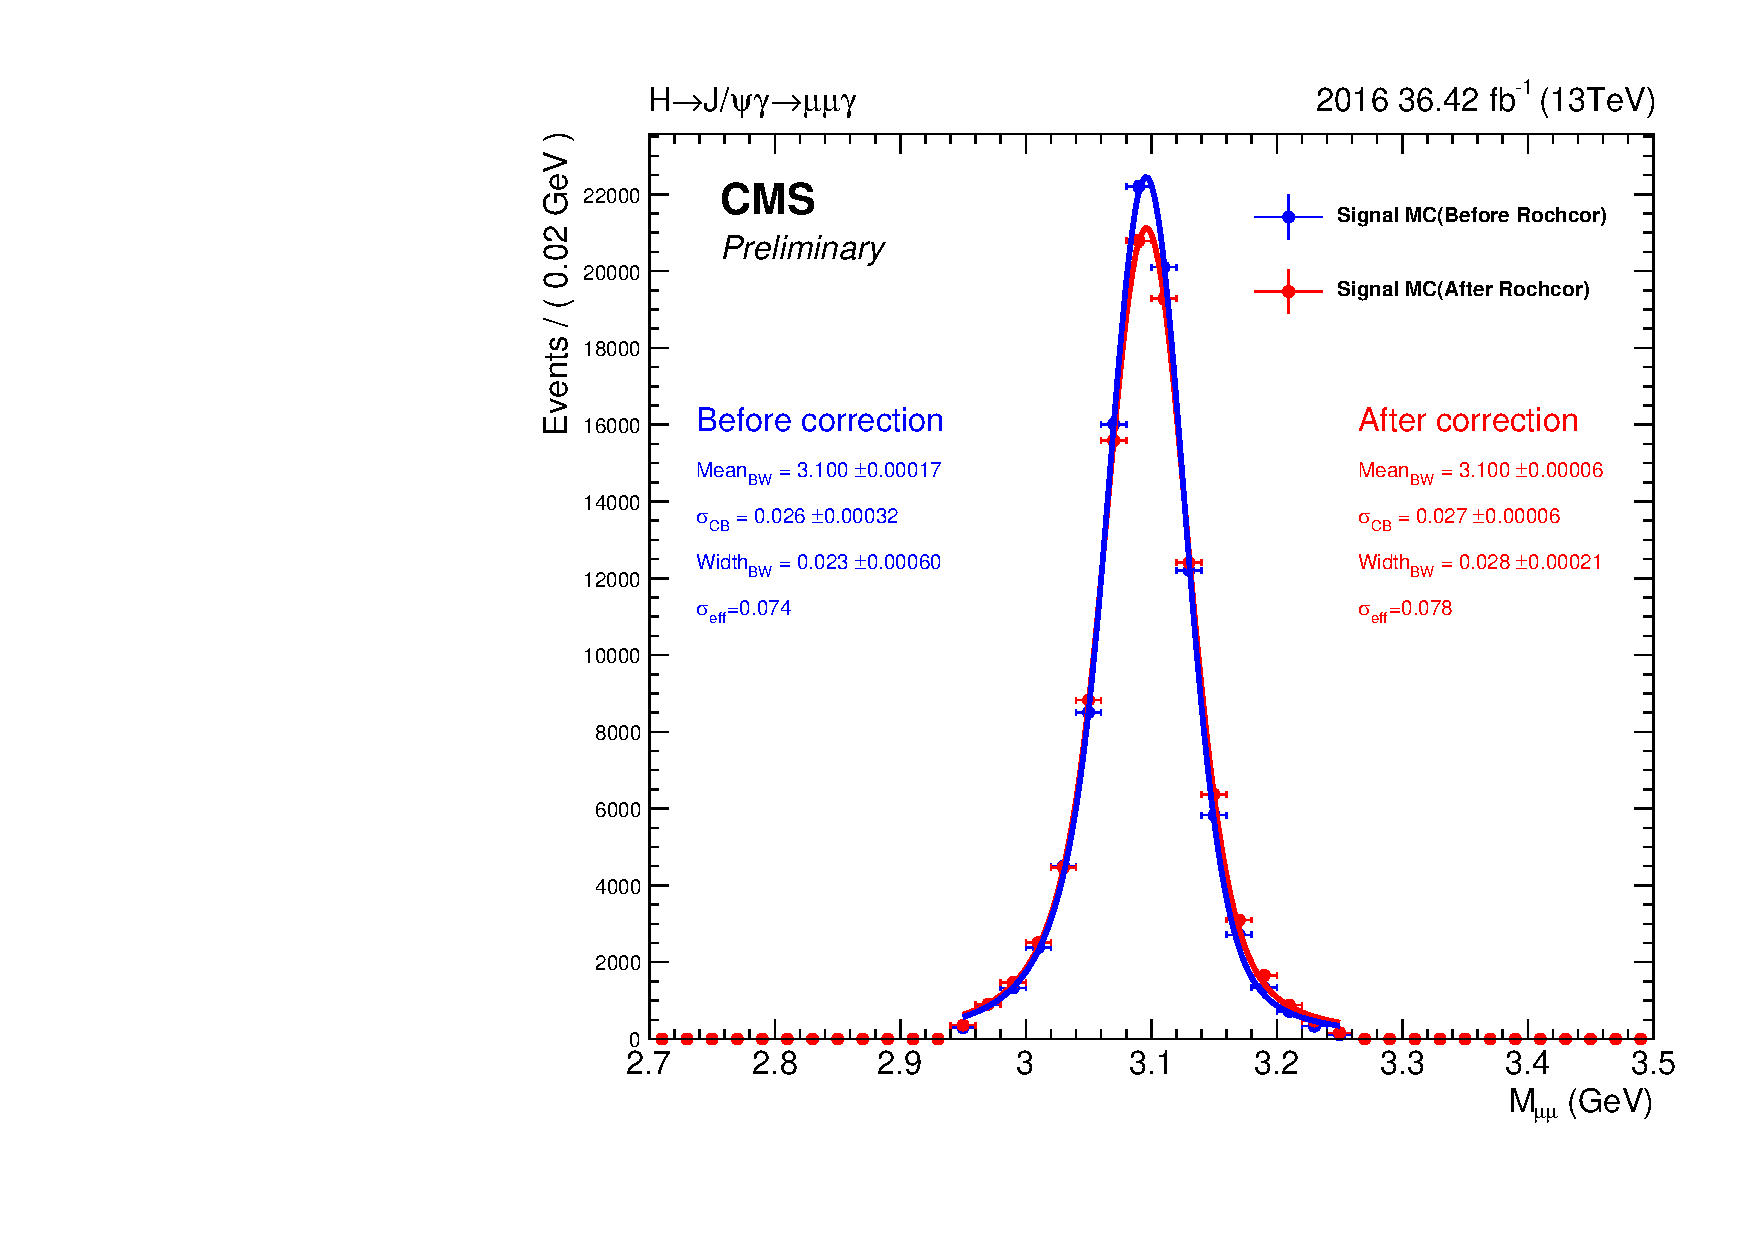
\includegraphics[width=0.45\textwidth]{Fig/Rochcor_forJpsi/mJpsi_Rochcor_BWConvCB_SignalMC}~
		  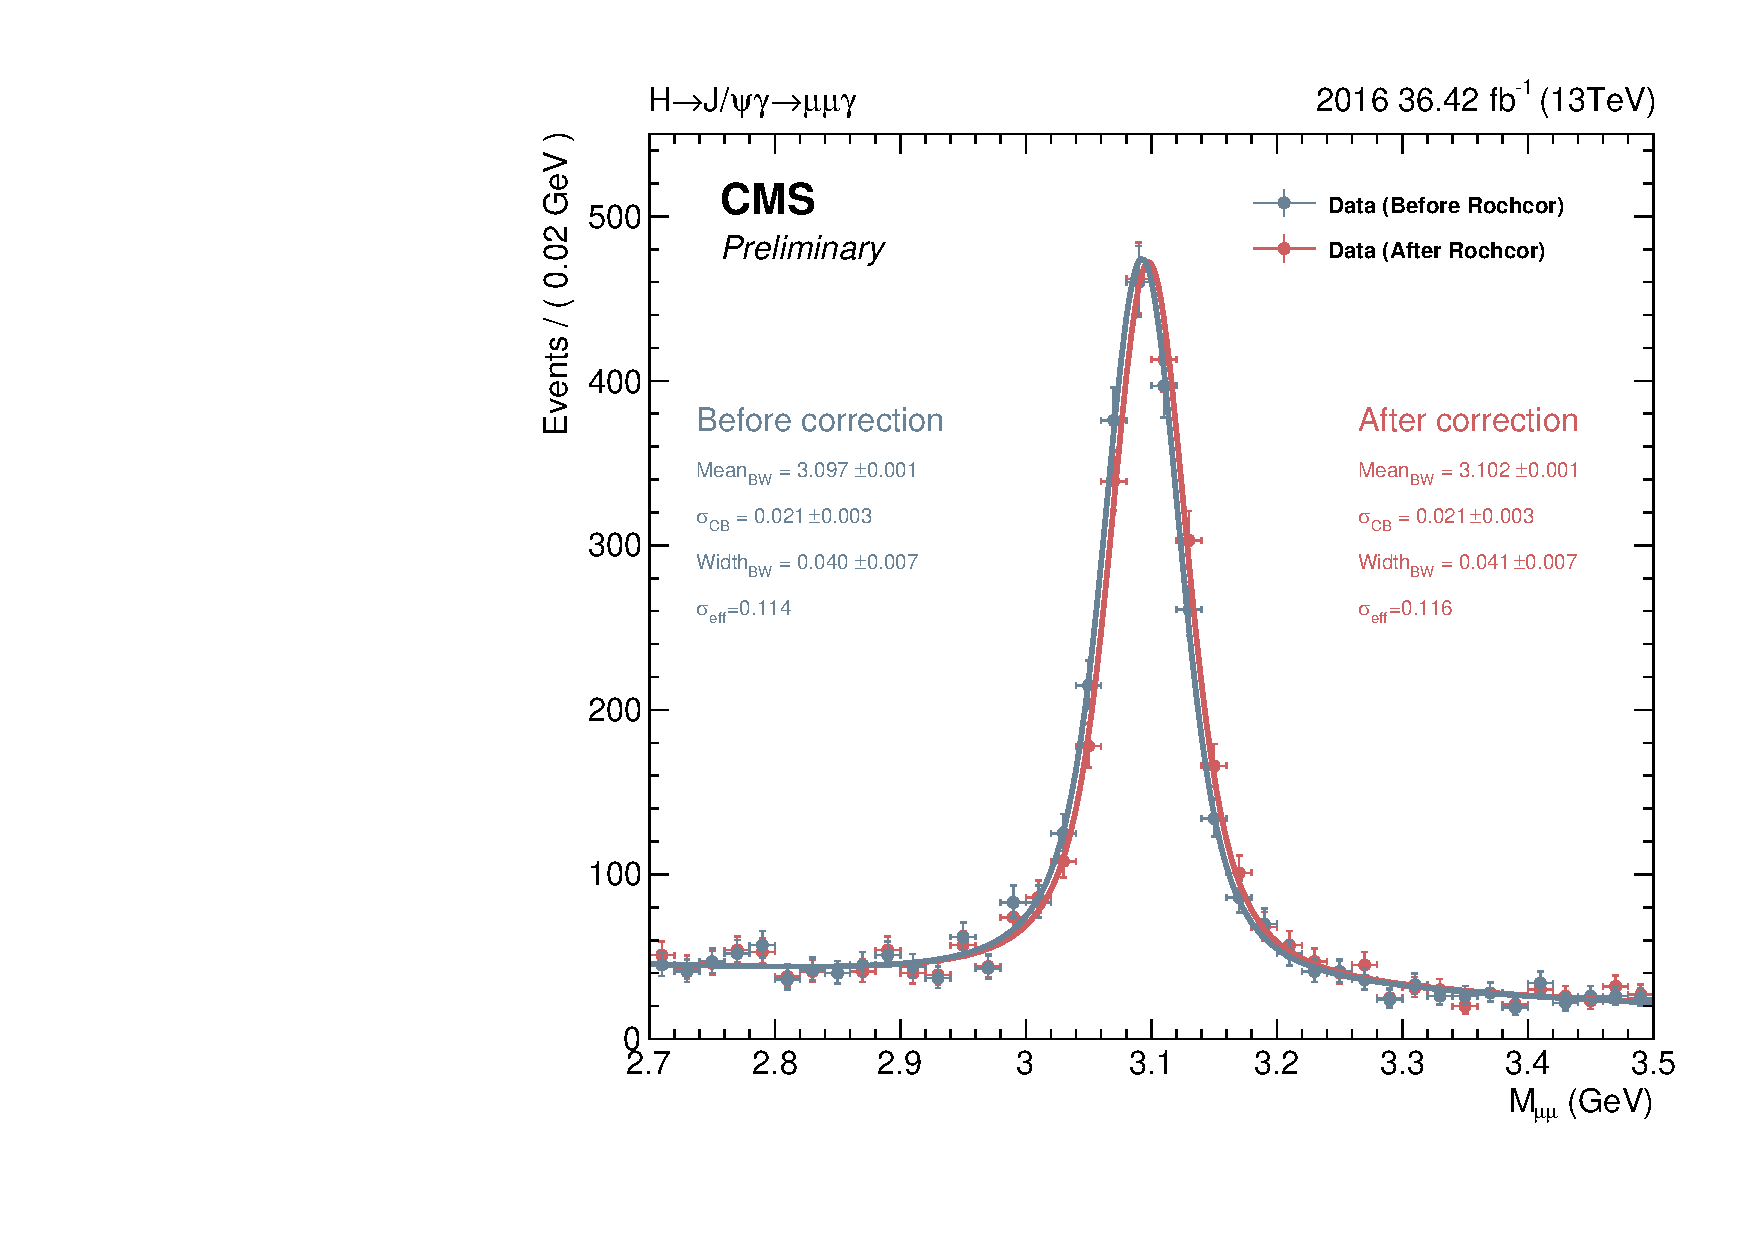
\includegraphics[width=0.45\textwidth]{Fig/Rochcor_forJpsi/mJpsi_Rochcor_BWConvCB}\\
		  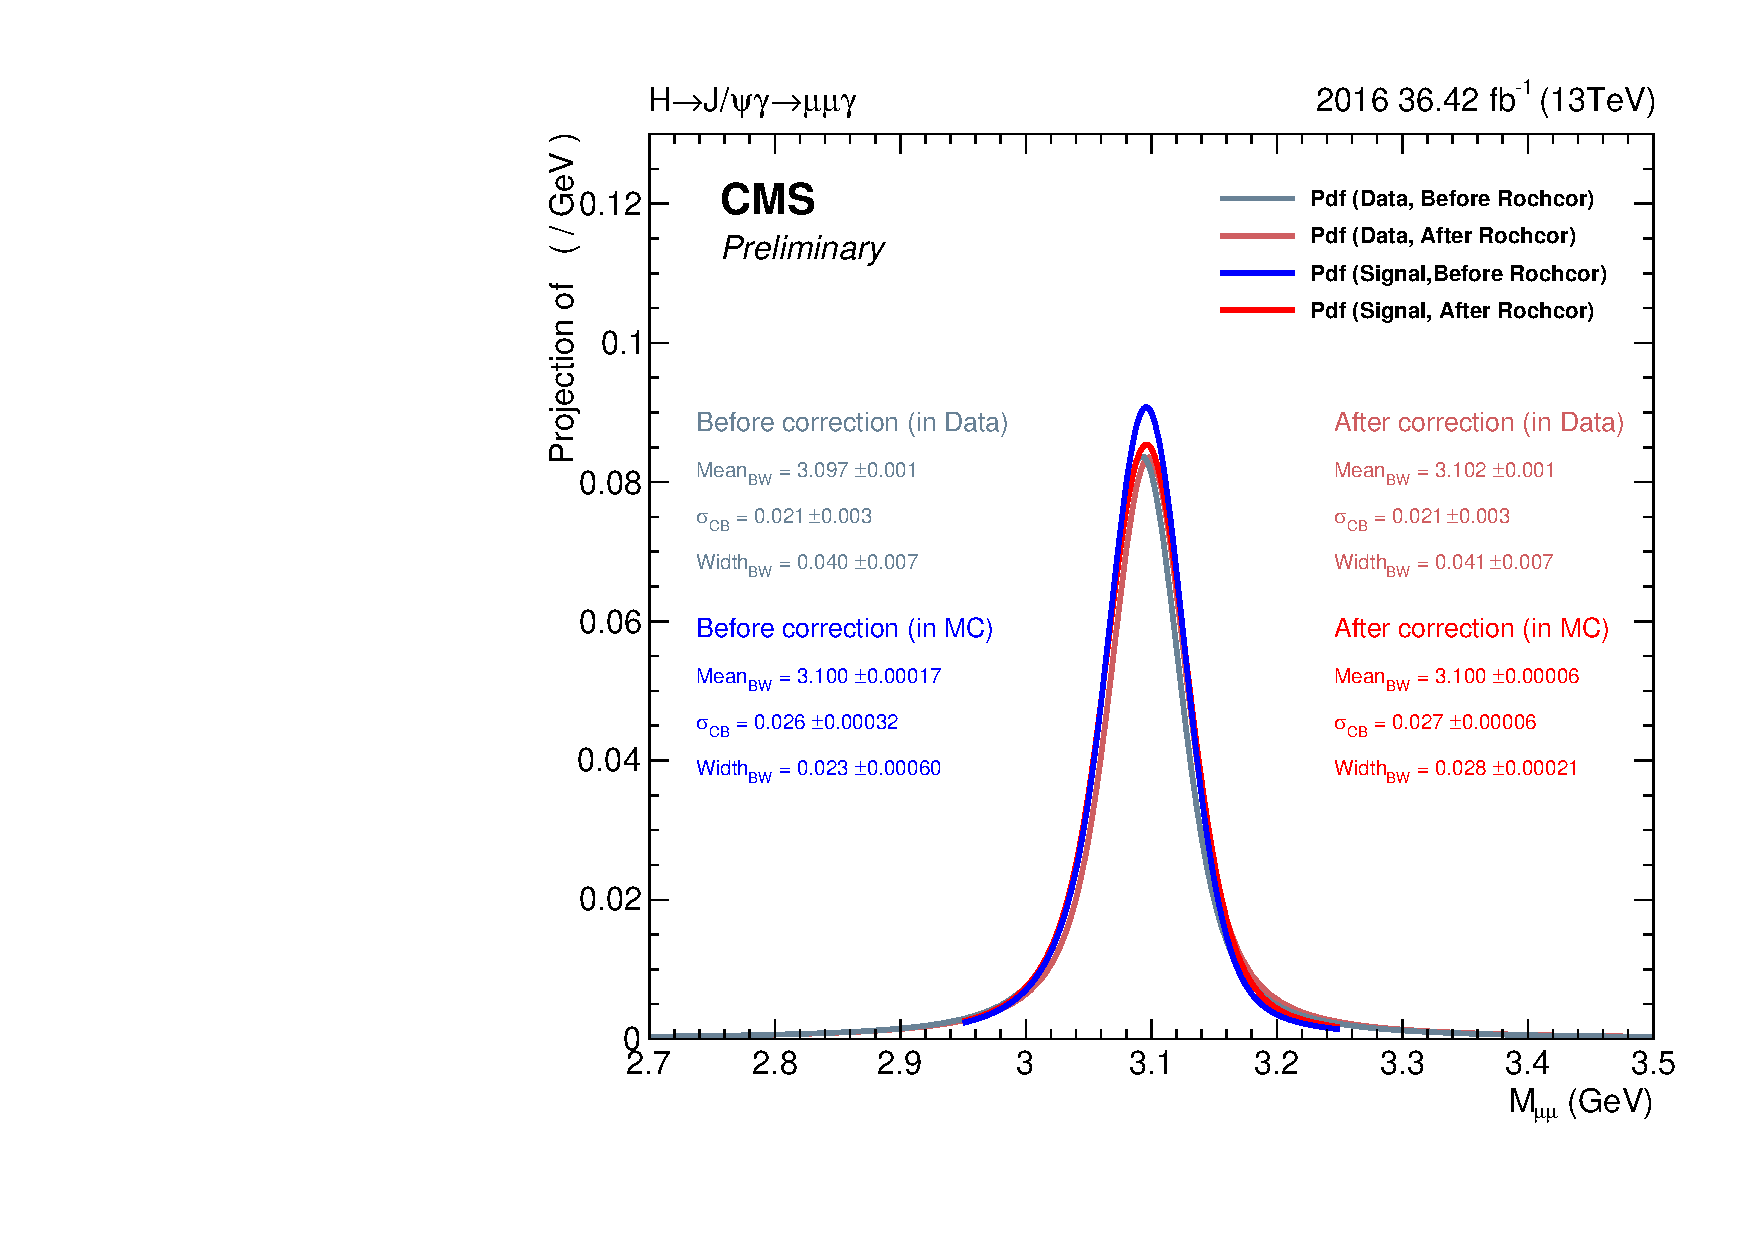
\includegraphics[width=0.45\textwidth]{Fig/Rochcor_forJpsi/mJpsi_Rochcor_BWConvCB_DataMC}\\
		  \caption{Comparisons between the dimuon mass $m_{\mu\mu}$ distributions with and without the corrections in both data and signal MC.}
		  \label{fig:RochcorForJpsi}
		\end{figure}
		
		\subsubsection{Muon efficiency measurements}
		A ``tag-and-probe`` method~\cite{cite:tagandprobe} based on samples of $\cPZ\to\mu\mu$ and $\JPsi\to\mu\mu$ events in data and simulation is used to measure the efficiency, and is found to be between 94--98 (92--97)\% in the barrel (endcap), depending on muon \pt and $\eta$. The isolation efficiency is measured with $\cPZ\to\mu\mu$ events, and found to be \pt dependent and between 90 (92) and 100\% in the barrel (endcap).
		
%		\textbf{Reconstruction and identification} \hspace{1cm} The $\cPZ$ sample is used to measure the muon reconstruction and identification efficiencies at high $\pt$ ($\pt>20\GeV$), and the efficiencies of the isolation and impact parameter requirements at all $\pt$. 
%		The $\JPsi$ sample is used to measure the reconstruction efficiency at low $\pt$ ($\pt<20\GeV$), as it benefits from a better purity in that kinematic regime. 
%		The reconstruction and identification efficiencies for $\pt>20\GeV$ are provided by the official measurement. The probe objects in this measurement are tracks reconstructed in the inner tracker, and the passing probe objects are those that are reconstructed as tracker or global muon and passing the official Loose identification\footnotemark. 
%		\footnotetext{The official Loose identification requires the muons must be particle-flow muons, and can either be global or tracker muons.} 
%		For the low-$\pt$ muons, the efficiencies are measure with $\JPsi\to\mu\mu$ with the same definitions of probes and passing probes. Fig.~\ref{fig:MuonRecoEff} shows the efficiencies at low $\pt$ as function of $\pt$ in the barrel (left) and endcaps (center), and as function of $\eta$ for $\pt>7\GeV$ (right). 
%		
%		\textbf{Tracking} \hspace{1cm} The efficiency to reconstruct a muon track in the inner detector is measured by using tracks reconstructed in the muon system alone as probes and those can be matched to at least one track as passing probes. Fig.~\ref{fig:MuonTrackEff} shows the efficiency as function of $\eta$ for muons with $\pt<10\GeV$ (left) and $\pt>10\GeV$ (right).
%		
%		\textbf{Impact parameter requirements} \hspace{1cm} The measurement is performed using $\cPZ$ events. The probes are muons passing the official Loose identification, and passing probes are those satisfy the impact parameter cuts of this analysis. Fig.~\ref{fig:MuonImpactEff} shows the efficiency of the muon impact parameter requirements as function of $\pt$ in the barrel (left) and endcaps (center), and as function of $\eta$ for $\pt>20\GeV$ (right).
%		
%		\textbf{Isolation requirements} \hspace{1cm} The measurement is performed using $\cPZ$ events. The probes are muons passing the identification requirements, and passing probes are those satisfy the isolation cut. Fig.~\ref{fig:MuonIsoEff} show the efficiency of the muon isolation requirement, as function of $\pt$ in the barrel (left) and endcaps (right).
%		
%		\begin{figure}[!ht]
%		  \centering
%		  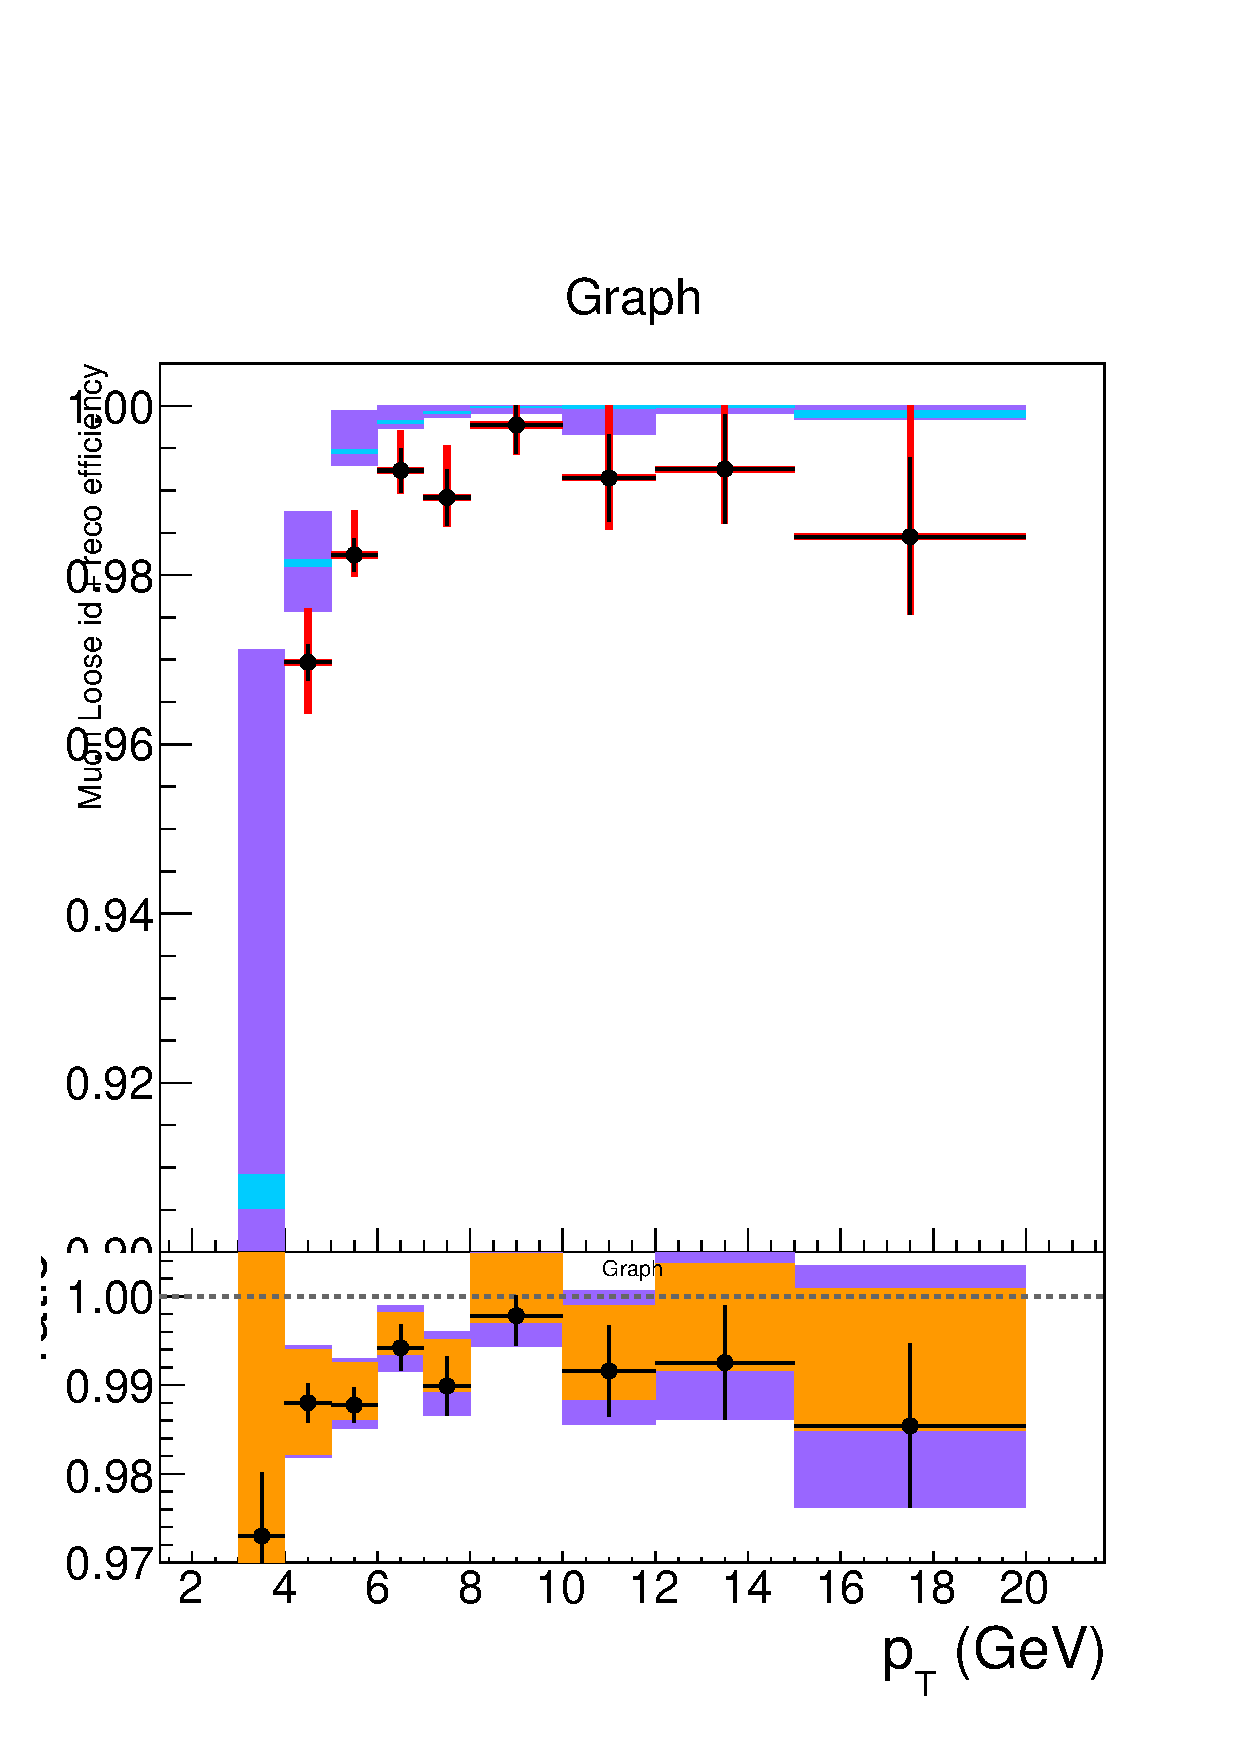
\includegraphics[width=0.3\textwidth]{Fig/MuonIDSF/mu_Loose_barrel}~
%		  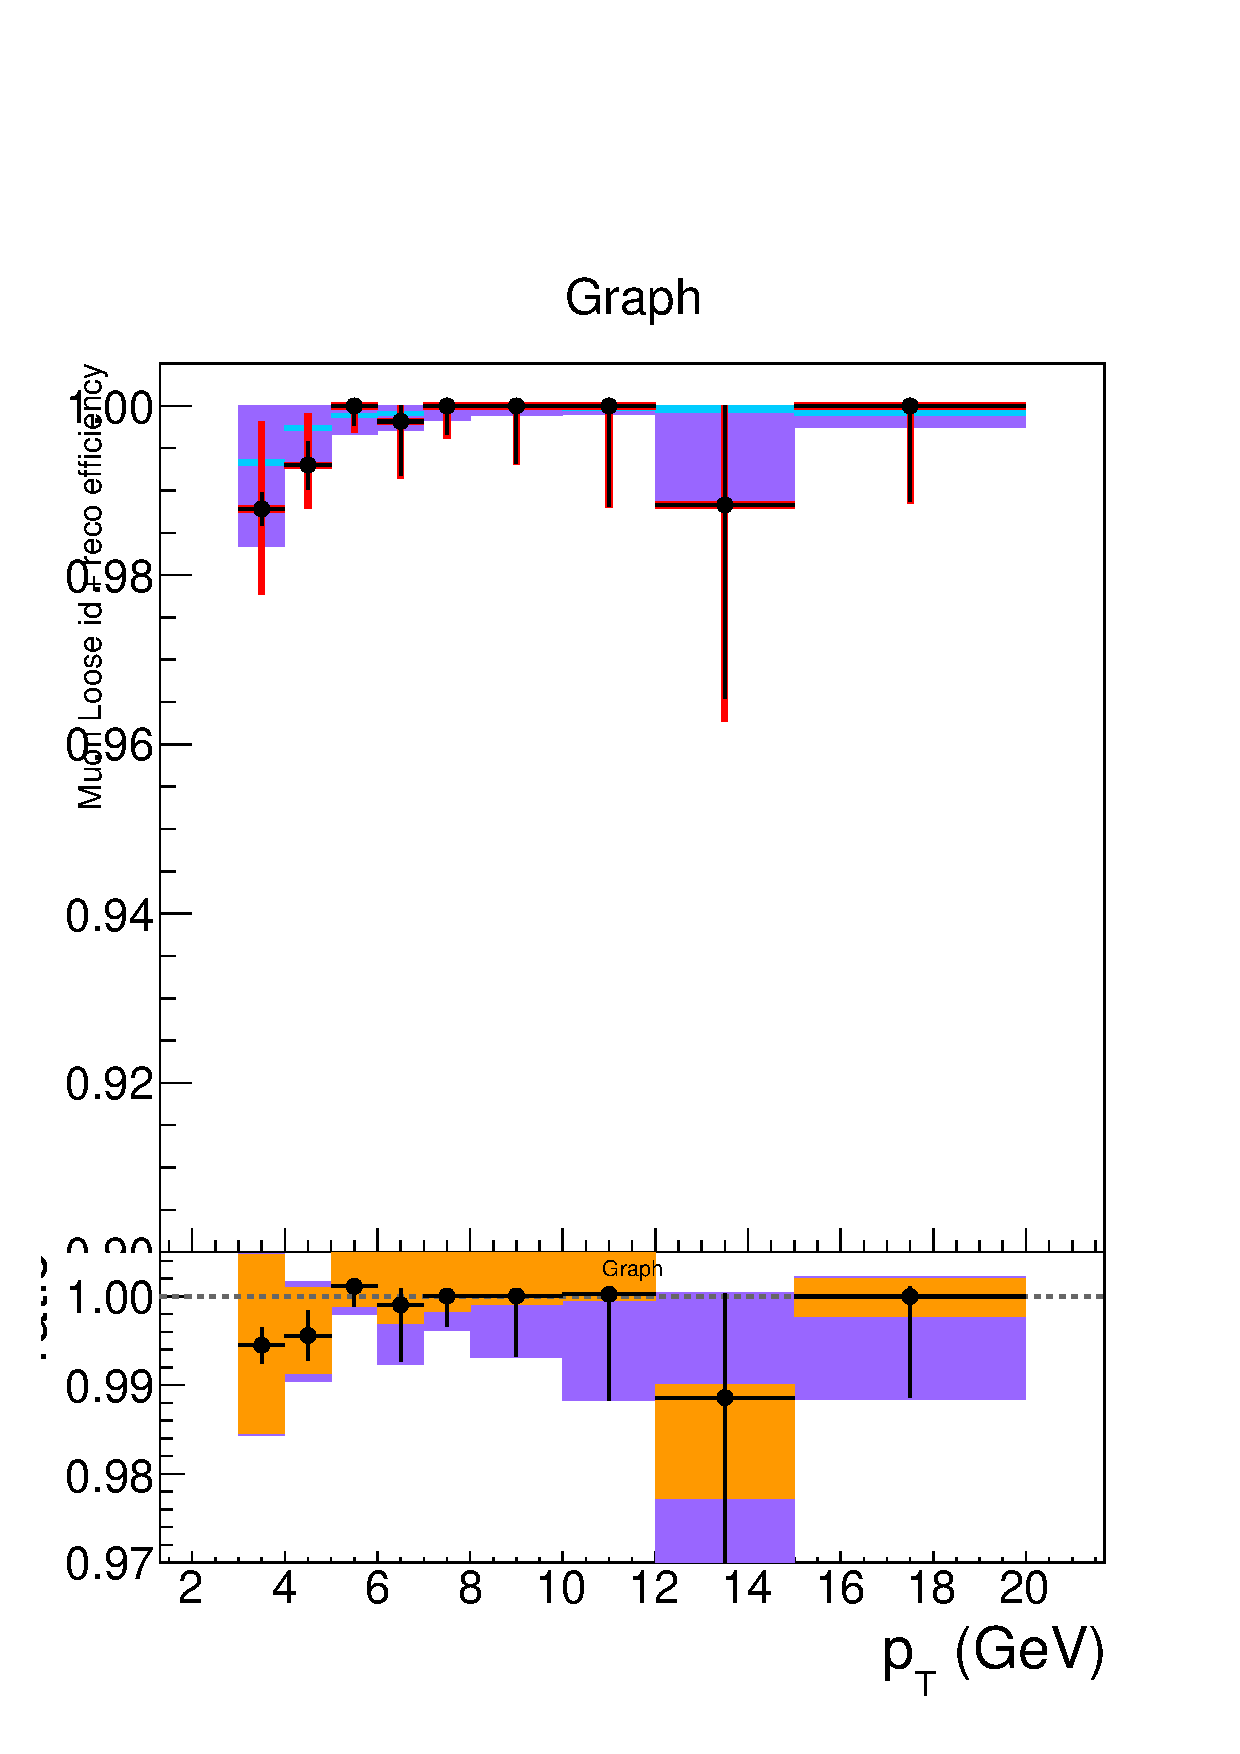
\includegraphics[width=0.3\textwidth]{Fig/MuonIDSF/mu_Loose_endcap}~
%		  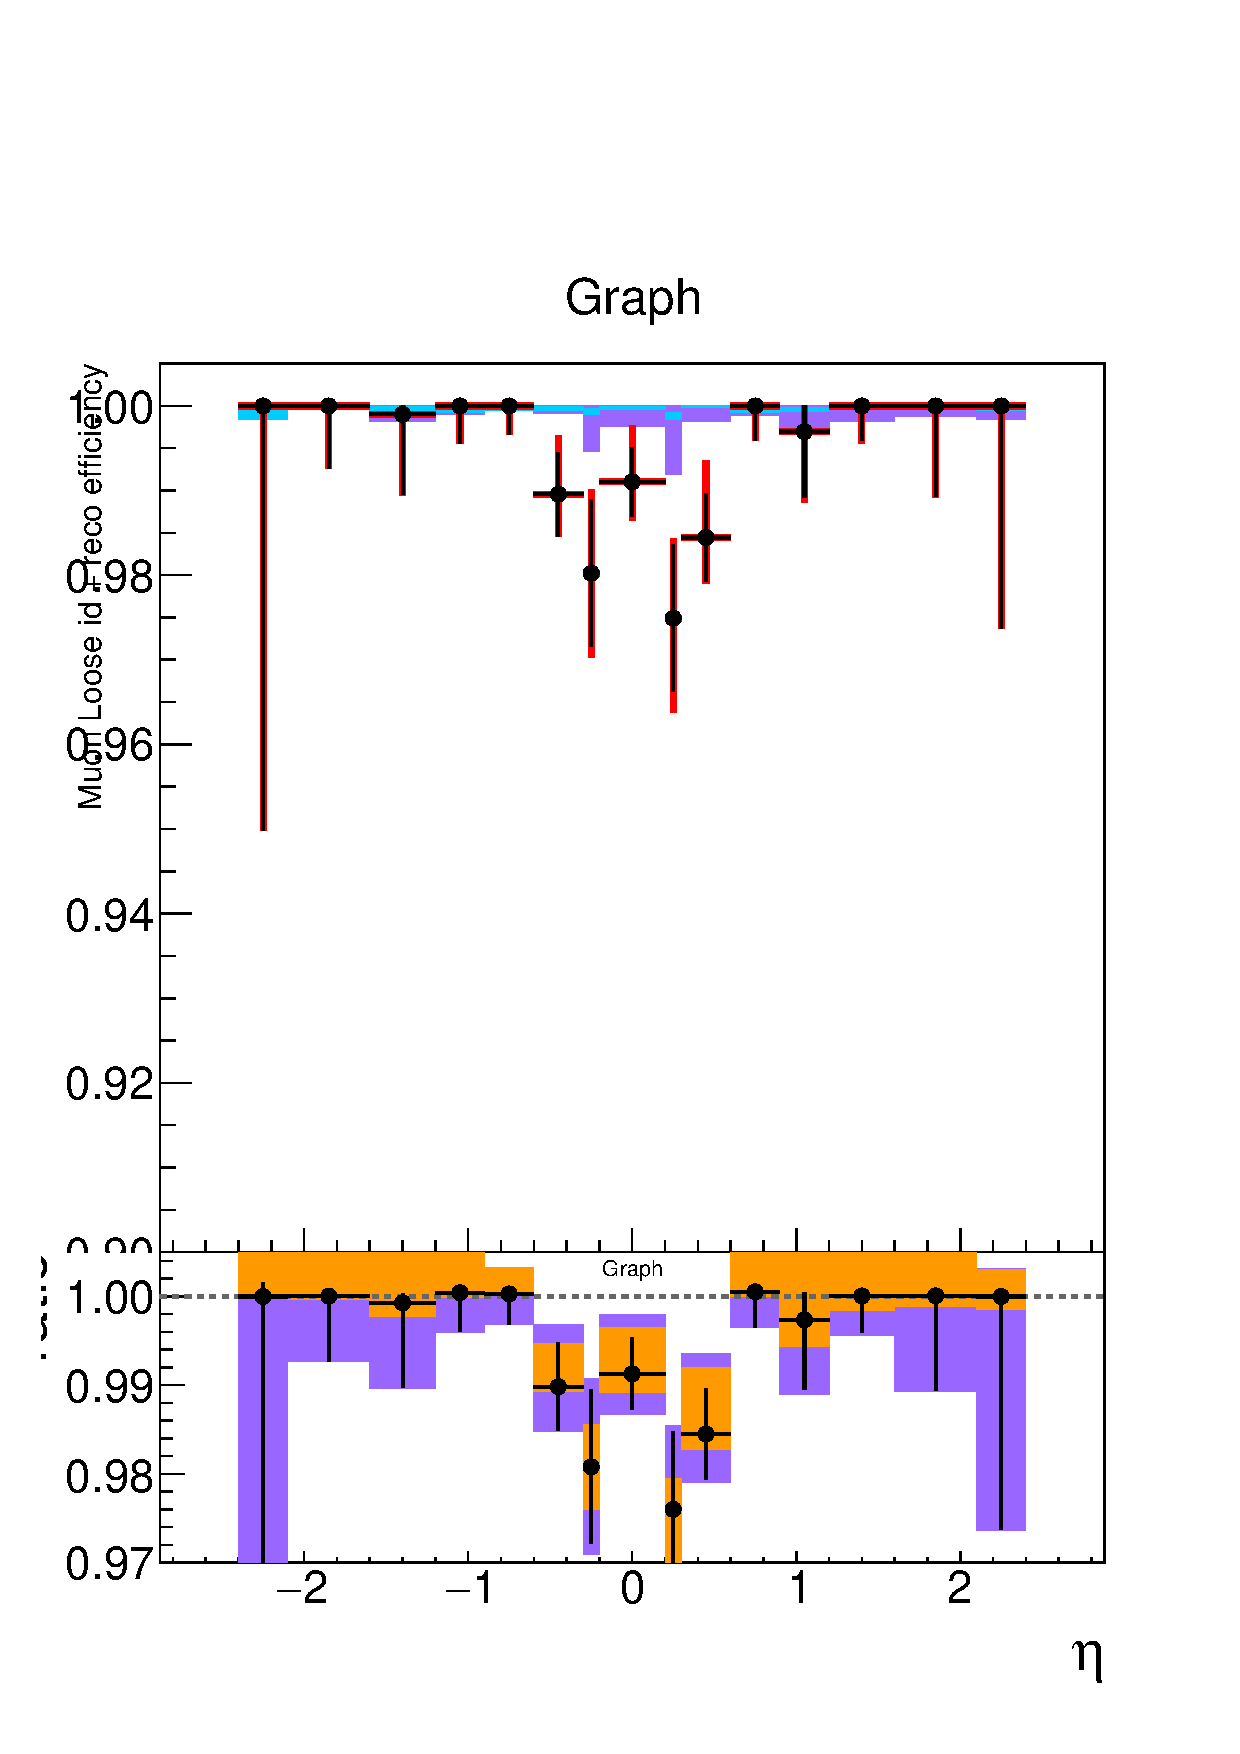
\includegraphics[width=0.3\textwidth]{Fig/MuonIDSF/mu_Loose_pt7}\\
%		  \caption{Muon reconstruction and identification efficiencies at low $\pt$ as function of $\pt$ in the barrel (left) and endcaps (center), and as function of $\eta$ for $\pt>7\GeV$ (right). In the upper panel, the larger error bars include the systematic uncertainties, while the smaller ones are statistical uncertainty only. In the lower panel showing the ratio of the two efficiencies, the black error bars are for the statistical uncertainty, the orange rectangles for the systematical uncertainty and the violet rectangles include both uncertainties.\label{fig:MuonRecoEff}}
%		\end{figure}	
%		
%		\begin{figure}[!ht]
%		  \centering
%		  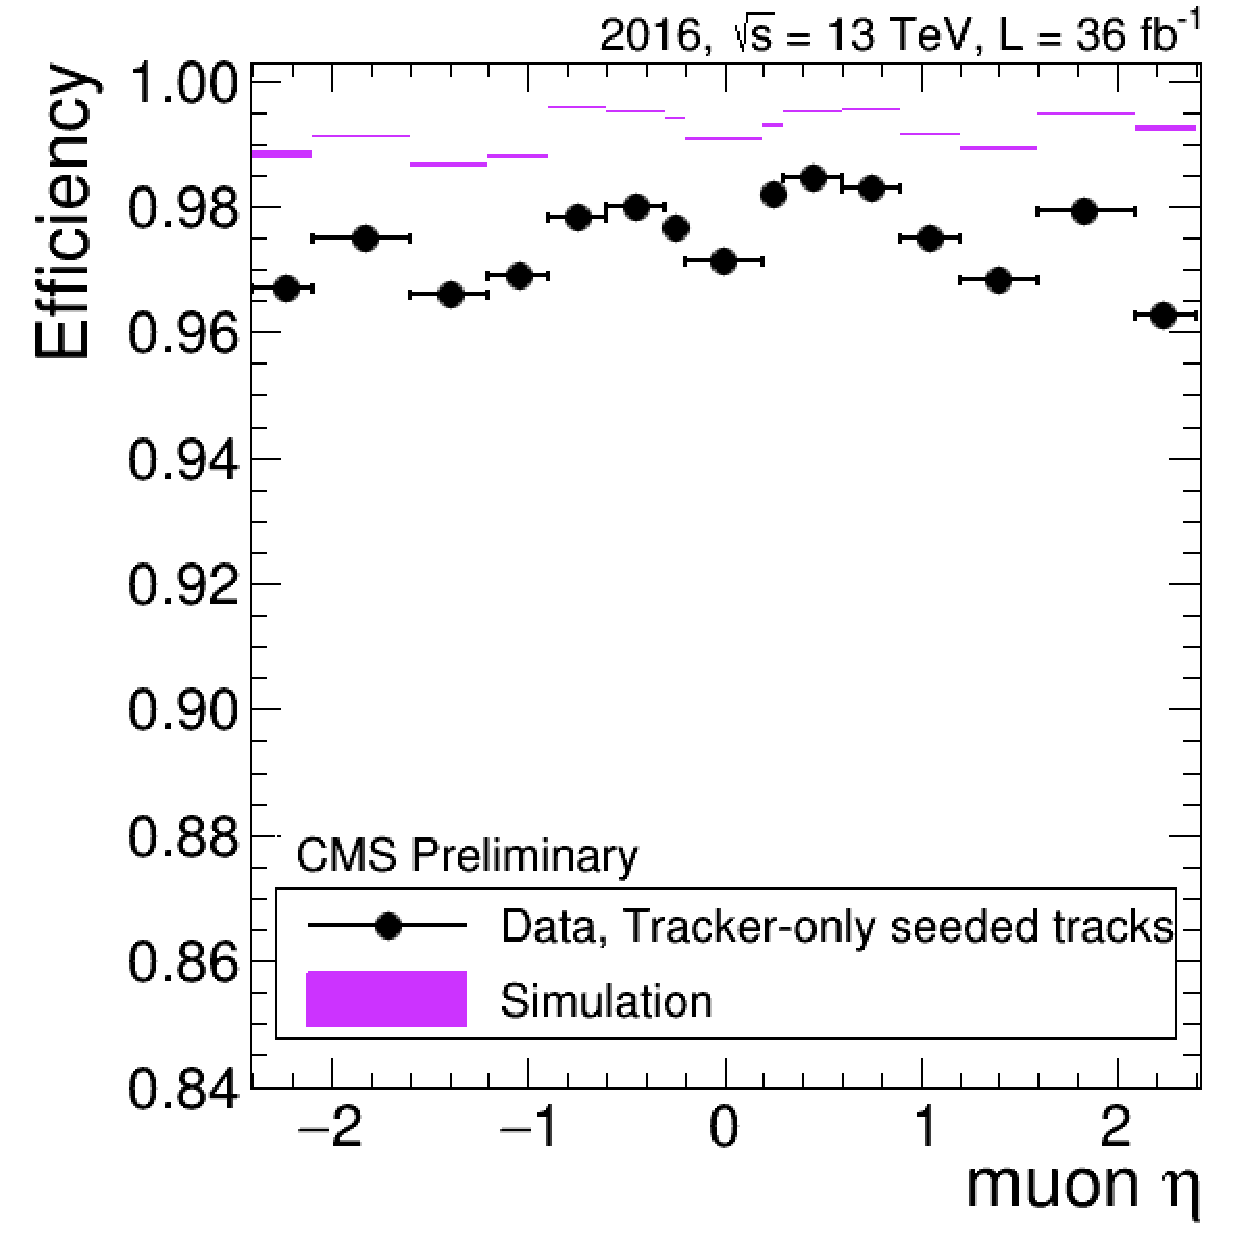
\includegraphics[width=0.3\textwidth]{Fig/MuonIDSF/trackingEffptl10}~
%		  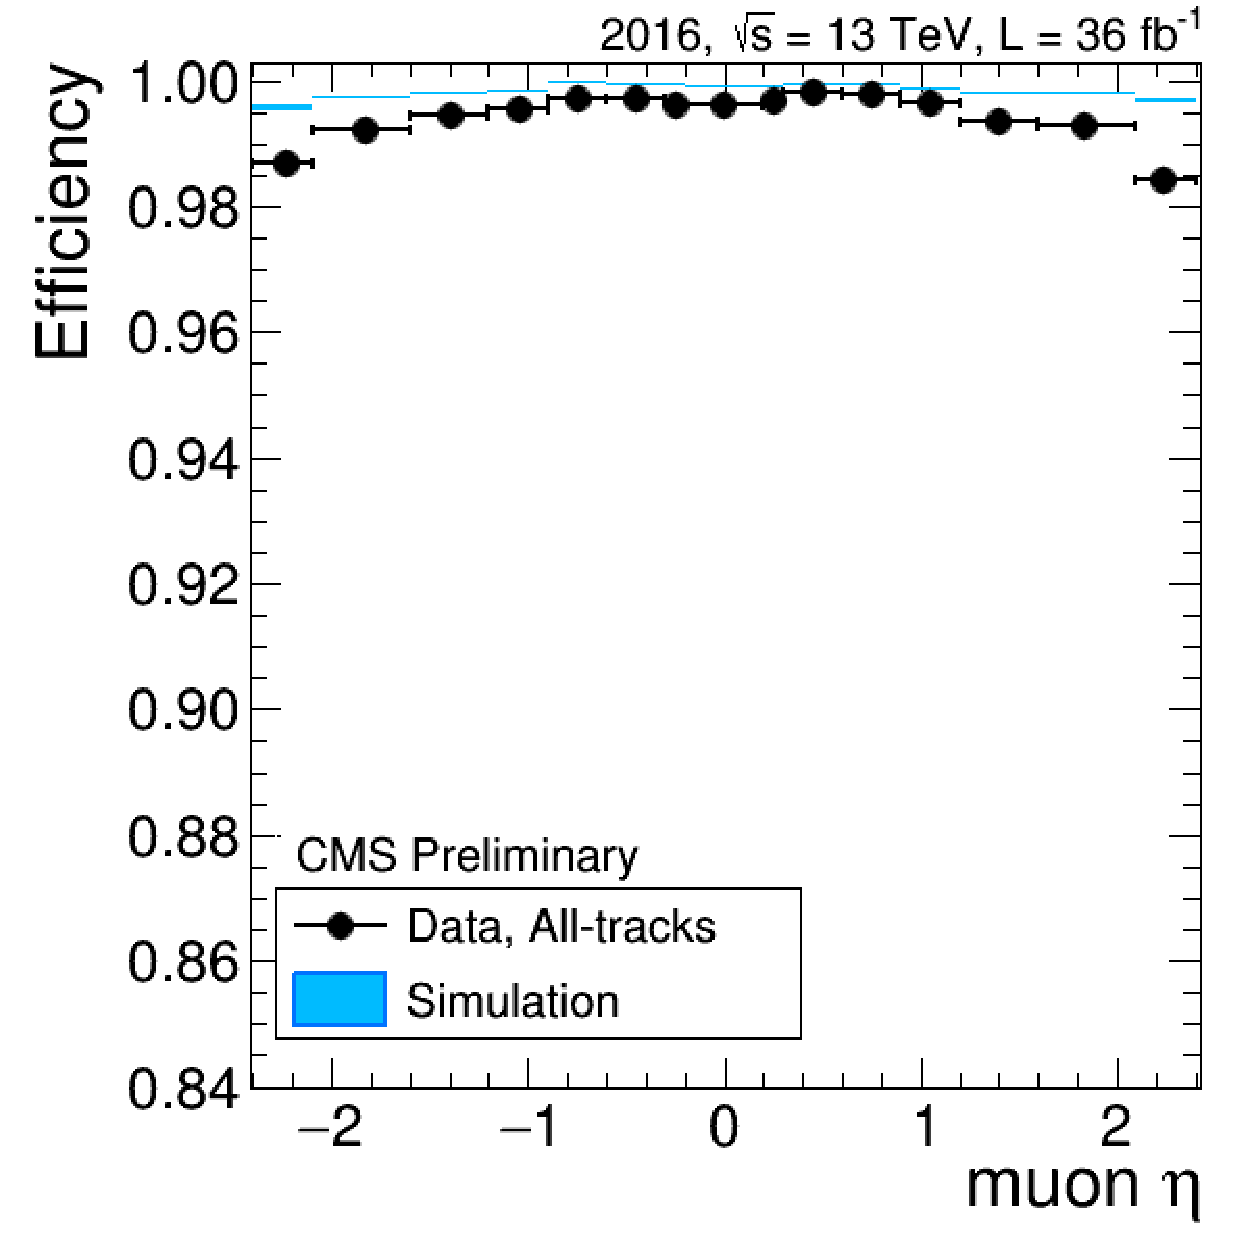
\includegraphics[width=0.3\textwidth]{Fig/MuonIDSF/trackingEffptg10}\\
%		  \caption{Muon tracking efficiency as function of $\eta$ for muons with $\pt<10\GeV$ (left) and $\pt>10\GeV$ (right). \label{fig:MuonTrackEff}}
%		\end{figure}
%		\clearpage
%		
%		\begin{figure}[!ht]
%		  \centering
%		  \includegraphics[width=0.3\textwidth]{Fig/MuonIDSF/mu_SIP4_barrel}~
%		  \includegraphics[width=0.3\textwidth]{Fig/MuonIDSF/mu_SIP4_endcap}~
%		  \includegraphics[width=0.3\textwidth]{Fig/MuonIDSF/mu_SIP4_pt20}\\
%		  \caption{Efficiency of the muon impact parameter requirements as function of $\pt$ in the barrel (left) and endcaps (center), and as function of $\eta$ for $\pt>20\GeV$ (right). \label{fig:MuonImpactEff}}
%		\end{figure}	
%		
%		\begin{figure}[!ht]
%		  \centering
%		  \includegraphics[width=0.3\textwidth]{Fig/MuonIDSF/mu_iso_barrel}~
%		  \includegraphics[width=0.3\textwidth]{Fig/MuonIDSF/mu_iso_endcap}\\
%		  \caption{Efficiency of the muon isolation requirement, as function of $\pt$ in the barrel (left) and endcaps (right). \label{fig:MuonIsoEff}}
%		\end{figure}	
%		\clearpage
		
		The difference in the efficiencies measured in simulation and data, which on average is 1\% per muon, is used to rescale the selection efficiency in the simulated samples. The products of all the data to simulation scale factors for muon tracking, reconstruction, identification, impact parameter and isolation requirements and corresponding uncertainties are shown in Fig.~\ref{fig:MuonSFs}.
		
		 \begin{table}[!ht]
		   \begin{center}
		     \begin{tabular}{|l|c|l|}
		       \hline
		       Reconstruction and identification & $\pt > 20\GeV$ & $Z\to\mu\mu$ events are used            \\
		       & $\pt < 20\GeV$ & $\JPsi\to\mu\mu$  events are used\\
		       \hline
		       Impact parameter         &  \multicolumn{2}{l|}{$Z\to\mu\mu$ events are used for the whole $\pt$ range}\\
		       \hline
		       Isolation    &        \multicolumn{2}{l|}{$Z\to\mu\mu$ events are used for the whole $\pt$ range}\\
		       \hline
		       Tracking     &        \multicolumn{2}{l|}{$Z\to\mu\mu$ events are used for the whole $\pt$ range}\\
		       \hline
		     \end{tabular}
		     \caption{The summary table of muon efficiencies and scale factors measurement. \label{tab:MuonIDSFs}}
		   \end{center}
		 \end{table}
		% \clearpage
		
		\begin{figure}[!htbp]
		  \centering
		  \includegraphics[width=1.0\textwidth]{Fig/MuonIDSF/Histogram_SFs_HZZID_FINAL}\\
		  \includegraphics[width=1.0\textwidth]{Fig/MuonIDSF/Histogram_SFs_HZZID_ERROR}\\
		  \caption{The histograms of overall data to simulation scale factors (reconstruction, identification, impact parameter and isolation requirements and tracking SF) and corresponding uncertainty.\label{fig:MuonSFs}}
		\end{figure}
		
		\subsection{Photon identification}
		\label{sec:pho}
		MVA based ID with working point (W.P) 90\% is used. 
		This ID is trained on a sample of simulated $\gamma+\text{jet}$ events, where the photon candidates matching the prompt photon are used as signal, and photon candidates not matching the prompt photon are identified as background.
		The input variables for the photon MVA training include the shower shapes variables, photon isolation, and charged hadron isolation. 
		The general purpose MVA has two categories, one for photons in barrel (EB) region and the other for those in endcap (EE) region. The suggested cut values, 0.2 for both categories, result in 95.2\% (93.9\%) of signal efficiency for $\cPZ\to\JPsi\ \gamma$ events and 60.3\% (67.3\%) of background rejection power, defined as $1-\epsilon_{\text{Bkg}}$, for the EB (EE) region. Here, the events selected in data are treated as background. 
		Fig.~\ref{fig:PhoMVAROC} shows the ROC curves for photon MVA ID obtained from $\cPZ\to\JPsi\ \gamma$ signal events and data events (treated and labeled as background in the plots), the point corresponding to the 90\% W.P for each category is shown as red solid star.
		
		\begin{figure}[!ht]
		  \centering
		  \includegraphics[width=0.49\textwidth]{Fig/PhoMVAIDSF/ROCcurve_phoMVA_ZJpsiG_EB}~
		  \includegraphics[width=0.49\textwidth]{Fig/PhoMVAIDSF/ROCcurve_phoMVA_ZJpsiG_EE}\\
		  \caption{The ROC curves for photon MVA ID obtained from $\cPZ\to\JPsi\ \gamma$ signal events and data events for EB (left) and EE (right) category. The red solid star corresponds to the efficiency for 90\% W.P. \label{fig:PhoMVAROC}}
		\end{figure}	
		
		The contamination of fake photons is estimated by checking the ratio of the $\cPZ+\text{jets}$ yields to the $\cPZ+\gamma$ yields. This gives a rough idea on the performance of photon ID. 
		It is found that the ratio of $\cPZ+\text{jets}$/$\cPZ\gamma$ events is $\sim 30\%$ for photon $\et$ between 33 and 40\GeV, and $\sim 20\%$ for photon $\et$ between 60 and 80\GeV. The ratios of $\cPZ+\text{jets}$/$\cPZ\gamma$ events in different photon $\et$ regions are summarized in Table~\ref{tab:fakephoratio}. 
		
		\begin{table}[!ht]
		    \begin{center}
		    \begin{tabular}{c|c}
		      photon $\et$  &  $\cPZ+$jets/$\cPZ\gamma$ (in \%)\\
		      \hline
		      $33<\et^{\gamma}<40\GeV$ & 30 \\
		      $40<\et^{\gamma}<50\GeV$ & 28 \\
		      $50<\et^{\gamma}<60\GeV$ & 22 \\
		      $60<\et^{\gamma}<80\GeV$ & 21 \\
		    \end{tabular}
		    \caption{The ratios of $\cPZ+$jets/$\cPZ\gamma$ events in different photon $\et$ regions.\label{tab:fakephoratio}}
		    \end{center}
		\end{table}
		
		Conversion safe electron veto (CSEV) is used to reject photons from electron conversions by requiring that there be no charged-particle track with a hit in the inner layer of the pixel detector associated to the photon cluster in the ECAL. The small number of inoperative sensors and possible cases where a track can pass between the first layer of sensors without leaving a hit are accounted for. The photon inefficiency is largely reduced and the residual comes from photons converting in the beam pipe. Up to 99.1\% (97.8\%) of photon in EB (EE) can pass CSEV, and 5.3\% (19.6\%) of electrons in EB (EE) can also satisfy this requirement. 
The efficiency of the photon identification is measured from $\cPZ\to\re\re$ events using tag-and-probe techniques, and found to be between 84 and 91\% (77 and 94\%), depending on the transverse energy $\et$, in the barrel (endcap). The electron veto efficiencies are measured with $\cPZ\to\mu\mu\gamma$ events, where the photon is produced by final-state radiation, and found to be 98 (94\%) in the barrel (endcap). The scale factors for the photon ID in bins of photon $\et$ and $\eta_{SC}$ are shown in Fig.~\ref{fig:PhotonMVASF}, and those for the CSEV are shown in Fig.\ref{fig:PhotonElevetoSFs}.	
		
%		\begin{figure}[p]
%		  \centering
%		  \includegraphics[width=0.75\textwidth]{Fig/PhoMVAIDSF/egammaEffi_egammaPlots_pT}\\
%		  \includegraphics[width=0.75\textwidth]{Fig/PhoMVAIDSF/egammaEffi_egammaPlots_SCEta}\\
%		  \caption{The efficiencies as a function of photon $\et$ (top) and of photon supercluster $\eta$ (bottom) in data, as well as the scale factors. \label{fig:PhotonMVAEff}}
%		\end{figure}
		
		\begin{figure}[!ht]
		  \centering
		  \includegraphics[width=0.96\textwidth]{Fig/PhoMVAIDSF/EGamma_SF2D}\\
		  \caption{The scale factors in bins of photon $\et$ and $\eta_{SC}$. \label{fig:PhotonMVASF}}
		\end{figure}
		
	%	\subsubsection*{$\text{R}_{\text{9}}$ reweighting}
	%	 $R_{9}$ variable is defined as the energy sum of 3x3 crystals centered on the most energetic crystal in the supercluster divided by the energy of the supercluster.
	%	Discrepancy between data and simulation were seen for the $R_{9}$ shower shape variable, shown in Fig.~\ref{fig:PhoR9}. The reweighting factors were applied to MC so that the $R_{9}$ distribution of MC will match to that of data~\cite{AN-17-036}.
		
	%	\begin{table}[h]
	%	    \begin{center}
	%	    \caption{The photon MVA identification input variables.}
	%	    \begin{tabular}{|c|c|c|}
	%	      \hline
	%	      Shower shape  & Isolation & Other \\
	%	      \hline
	%	      $R_{9}$ & CITK Photon isolation & $\eta_{SC}$\\
	%	      S4 & CITK Charged isolation & $E_{SC}^{Raw}$\\
	%	      $\sigma_{i\eta i\eta}$ & VID Charged isolation & $\rho$ \\
	%	      $\eta_{SC}$ width & & $E_{n}^{ES}/E^{Raw}$ \\
	%	      $\phi_{SC}$ width & & \\
	%	      \textit{$cov_{i\eta i\phi}$} & & \\
	%	      $ES\sigma_{RR}$ & & \\
	%	      $\phi$ & & \\
	%	      \hline
	%	    \end{tabular}
	%	    \label{tab:phoMVAID_inputvars}
	%	    \end{center}
	%	\end{table}
		
		\begin{figure}[!ht]
		  \centering
		  \includegraphics[width=0.5\textwidth]{Fig/PhoMVAIDSF/h_Scaling_Factors_CSEV_R9Inc}\\
		  \caption{The scale factors of SCEV in bins of photon $\eta_{SC}$.}
		  \label{fig:PhotonElevetoSFs}
		\end{figure}
		
		\section{Event Selection}  
		\label{subsec:KS}
		In addition to the object identification and isolation, kinematic selections are applied to further discriminate the background.
		\begin{itemize}
		\item Two opposite charged muons with $\pt^{\mu_{1}} > 20\GeV,\ \pt^{\mu_{2}} > 4\GeV,\ \left|\eta^{\mu}\right| < 2.4$. The $\pt$ cut value on the leading muon is driven by the trigger threshold. 
		\item $\JPsi$ candidate selection $3.0 < m_{\mu\mu} < 3.2\GeV$.
		\item $\et^{\gamma} > 33\GeV$, $\left|\eta_{SC}^{\gamma}\right| < 2.5$, excluding the Barrel-Endcap transition region at $1.4442 < \left|\eta_{SC}^{\gamma}\right| < 1.566$. The $\et$ cut value on the photon is driven by the trigger threshold.
		\item $\Delta R(\mu_{1},\gamma) > 1$, $\Delta R(\mu_{2},\gamma) > 1$, $\Delta R(\mu\mu,\gamma) > 2$, and $|\Delta\phi(\mu\mu,\gamma)| > 1.5$. The angular separation $\Delta R$ cuts on each muon and the photon are imposed to suppress Drell-Yan process with FSR photon. As we do not have proper background MC samples, the cut values are determined such that a higher total signal efficiency is kept.  
		\item $\pt^{\mu\mu},\et^{\gamma} / m_{\mu\mu\gamma} > 0.28$ (35/125) for $\PH\to\JPsi\ \gamma$), 0.384 (35/91.2) for $\cPZ\to\JPsi\ \gamma$. If a hard cut on $\et$ or $\pt^{\mu\mu}$ is imposed, there will be an obvious turn-on at the $\cPZ$ mass region, as shown in Fig.~\ref{fig:invariantmass}, which will complicate the background model. This ratio cut also helps to reject the $\gamma^*+$jet and $\gamma+$jet backgrounds. As for the cut value, 91.2 and 125.0\GeV are the nominal mass of the $\cPZ$ and Higgs boson respectively.
		\end{itemize}
		
		\begin{figure}[!ht]
		  \centering
		  \includegraphics[width=0.7\textwidth]{Fig/Mmmg_Various}\\
		  \caption{$m_{\mu\mu\gamma}$ distributions with different forms of $\pt$ or $\et$ cuts. \label{fig:invariantmass}}
		\end{figure}
		
		Table~\ref{tab:FullSelec} summarizes event selections in this analysis
		\begin{table}[!ht]
		    \begin{center}
		    \begin{tabular}{l}
		      \hline
		      Trigger : HLT\_Mu17\_Photon30\_CaloIdL\_L1ISO\_v\* \\
		      \hline
		      Muon identification,  Particle Flow Isolation in cone 0.3 for $\mu_{\text{lead}} < 0.35$\\ 
		      $\pt^{\mu_{\text{lead}}} > 20\GeV$, $\pt^{\mu_{\text{trai}}} > 4\GeV$, $|\eta_{\mu}| < 2.4$ \\
		      \hline
		      Photon MVA ID(90$\%$ WP), $\et^{\gamma} > 33\GeV$ \\
		      $|\eta_{SC}^{\mu}| < 2.5$, excluding those in Barrel-Endcap transition region of ECAL.\\
		      \hline
		      $\Delta R(\mu_{1},\gamma) > 1$, $\Delta R(\mu_{2},\gamma) > 1$, $\Delta R(\mu\mu,\gamma) > 2$, and $|\Delta\phi(\mu\mu,\gamma)| > 1.5$ \\
		      \hline
		      $3.0 < m_{\mu\mu} < 3.2\GeV$ \\
		      \hline
		      $\pt^{\mu\mu} / m_{\mu\mu\gamma} >  0.384 (0.28), \et^{\gamma} / m_{\mu\mu\gamma} > 0.384  (0.28)$ for the $\cPZ\ (\PH)\to\JPsi\ \gamma$. \\
		      \hline
		    \end{tabular}
		    \caption{The selection requirements in this analysis, including ID, isolation and kinematic selection.\label{tab:FullSelec}}
		    \end{center}
		\end{table}
		
	In the $\cPZ\to\JPsi\ \gamma$ search, selected events are classified into mutually exclusive categories in order to enhance the sensitivity of the search. The categorization is based on the $\eta$ of the photon and the photon $\RNINE$ variable (defined as the energy sum of 3$\times$3 ECAL crystals centered on the most energetic crystal in the supercluster divided by the energy of the supercluster). Unconverted photons have high values of $\RNINE$ and a threshold of 0.94 is used to classify reconstructed photons with high $\RNINE$ (thus with a better resolution) and low $\RNINE$ (worse resolution).  The background is larger in the converted photon category.  The three categories are: photon in the barrel region with a high $\RNINE$ value (referred to as EB high $\RNINE$); photon in the barrel region with low $\RNINE$ value (referred to as EB low $\RNINE$); photon in the endcap region (referred to as EE). The EE category is not divided into high/low $\RNINE$ because there are few events in this category. By this categorization, this improvement on the search limit is $\sim 2.0\%$.
	In the $\PH\to\JPsi\ \gamma$ search events are not divided into categories. The possibility of splitting the EE category was investigated, but this did not result in a significant improvement.	
		
		The exact definition of the three event categories in $\cPZ\to\JPsi\ \gamma$ search are shown in Table~\ref{tab:2}.
		The table includes the fractions of expected events in each category for signal and of the observed events for data. The $\sigma_{\text{eff}}$ of the $m_{\mu\mu\gamma}$ distribution of each category is also included. 
		
		\begin{table}[!ht]
		\small
		\begin{center}
		\begin{tabular}{cccc}
		\hline
		           & Category 1  & Category 2 & Category 3\\
		           \cline{2-4}
		           & $0<|\eta_{\gamma}^{SC}|<1.4442$ & $0<|\eta_{\gamma}^{SC}|<1.4442$ & $1.566<|\eta_{\gamma}^{SC}|<2.5$ \\
		           & $R_{9} > 0.94$ & $R_{9} > 0.94$ & - \\
		           \hline
		Data & 40.3\% & 36.2\% & 23.5\% \\
		Signal & 49.0\% & 30.6\% & 20.3\% \\
		$\sigma_{\text{eff}}$&  3.58\GeV & 3.86\GeV & 4.08\GeV\\                                                                      
		\hline
		    \end{tabular}
		    \caption{Definition of the three event classes in $\cPZ\to\JPsi\ \gamma$ and the fraction of selected events in signal and data. The expected mass resolution on the signal are also shown.\label{tab:2}}
		  \end{center}
		\end{table}
		
		Table~\ref{tab:Cutflow} summarizes the expected number of events from signals and observed yields in data in steps of event selection of both the Higgs and $\cPZ$ boson decays. For the $\cPZ$ boson decays, the numbers are with the unpolarized $\JPsi$ assumption and $\pt$ reweighting.
		Table~\ref{tab:ZyieldComp} shows the impacts of different polarization scenarios and the $\Z\ \pt$ reweighting. The variations on the yields resulting from the extreme polarization assumption is -7.8$\%$ (transverse) to +16$\%$ (longitudinal), corresponding to the total signal efficiency varying from 13.1\% to 16.4\%.
	The $\cPZ\ \pt$ reweighting, with weights derived from the $a\MCATNLO$ sample, results in +2.3$\%$ of increase on the expected yields of the $\cPZ$ decay. The difference between the yield with weights derived from the $a\MCATNLO$ sample and that from $\POWHEG$ is only 0.13$\%$, and no additional uncertainty is assigned.
		In both Z and Higgs decays the number of events coming from the peaking background $\PH\ (\cPZ)\to\mu\mu\gamma$ is large compared to signal processes. On the other hand, it is small compared to the total background. Hence, it has minimal effect on the upper limit on $\mathcal{B}(\PH\ (\cPZ)\to\JPsi\ \gamma)$.
		With the constraint $100\ (70) < m_{\mu\mu\gamma} < 150\ (120)\GeV$, the total signal efficiency, including kinematic acceptance, trigger and reconstruction efficiencies, and $\pt$ reweighting for the $\cPZ$ boson decay, of about 22.6\% and 14.2\% in Higgs and $\cPZ$ boson decays. 
		The difference in the total signal efficiency between the Higgs and the $\cPZ$ boson decay is mostly due to the kinematic acceptance, which comes from the difference in $\pt$ distributions of muons and photon given that the $\cPZ$ boson is lighter than the Higgs boson.
		
\begin{table}[!ht]
	\scriptsize
	\begin{center}
	  \begin{tabular}{ccccccc}
	  \hline
	    & \multicolumn{3}{c}{$\PH\rightarrow\JPsi\ \gamma$}  & \multicolumn{3}{c}{$\cPZ\rightarrow\JPsi\ \gamma$}\\
	    \cline{2-7}
	    & Data & $\PH\rightarrow\JPsi\ \gamma$ & $\PH\rightarrow\gamma^{*}\gamma$ & Data &  $\cPZ\rightarrow\JPsi\ \gamma$ & $\cPZ\to\mu\mu\gamma$\\
	    &      &  signal                    &  background                    &      & signal & background\\
	    \hline
	    Total (Before selection)& 170M & 0.350 & 91.7 & 170M & 10.8 & 3335\\
	    HLT & 30.3M & 0.190 & 51.3 & 30.3M & 4.24 & 1932\\
	    Muon selection & 650K & 0.136 & 35.9 & 650K & 2.67 & 1317\\
	    Photon selection & 152K & 0.116 & 30.7 & 152K & 2.17 & 1066 \\
	    $\Delta R$, $\Delta\phi$ & 59.4K & 0.101 & 23.5 & 59.4K & 2.09 & 1020\\
	    $m_{\mu\mu}$ & 1088 & 0.0929 & 0.274 & 1088 & 1.93 & 5.29\\
	    $m_{\mu\mu\gamma}$& 363 & 0.0928 & 0.273 & 637 & 1.90 & 5.37 \\
	    $\pt^{\mu\mu},\et^{\gamma}/m_{\mu\mu\gamma}$ & 279 & 0.0884 & 0.257 & 384 & 1.58 & 4.57 \\
	    \hline
	    \multicolumn{6}{c}{Expected signal yields (with the pileup weight, all the scale factors and efficiencies)}\\
	    \hline
	    All & 279 & 0.0765 & 0.207 & 384 & 1.54 & 4.47\\
	    Cat1 & \multicolumn{3}{c}{-} & 148 & 0.770 & 2.14\\
	    Cat2 & \multicolumn{3}{c}{-} & 144 & 0.468 & 1.20\\
	    Cat3 & \multicolumn{3}{c}{-} & 92 & 0.299 & 1.12\\
	    \hline
	  \end{tabular}
	    \caption{The expected signal yield and the number of selected events in data, for the integrated luminosity of 35.9$\fbinv$.\label{tab:Cutflow}}
	\end{center}
	\end{table}
	
	\begin{table}[!ht]
	\small
	  \begin{center}
	    \begin{tabular}{lcc}
	    \hline
	        &  \multicolumn{2}{c}{Inclusive}\\ 
	      	\cline{2-3}
	        & Yield & Difference (in $\%$) \\
	        \hline
	        \textbf{unpolarized} \& \textbf{with} $\pt$ reweighting   & 1.54   &    \\
	      	\textbf{transverse}ly polarized \& \textbf{with} $\pt$ reweighting   & 1.42   & -7.86   \\
	      	\textbf{longitudinal}y polarized \& \textbf{with} $\pt$ reweighting   & 1.78   & +15.7   \\
	      	\textbf{unpolarized} \& \textbf{without} $\pt$ reweighting   & 1.50   &   -2.24 \\
	      	\textbf{transverse}ly polarized \& \textbf{without} $\pt$ reweighting   & 1.38   & -9.85   \\
	      	\textbf{longitudinal}y polarized \& \textbf{without} $\pt$ reweighting   & 1.74   & +13.0   \\
	      	\hline
	    \end{tabular}
	    \caption{Summary of the impacts of different polarization scenarios and the $\cPZ$ $\pt$ reweighting.\label{tab:ZyieldComp}}
	  \end{center}
	\end{table}
	
	\begin{table}[h]
	\scriptsize
	\begin{center}
	  \begin{tabular}{ccccccc}
	  \hline
	    & \multicolumn{6}{c}{$\PH\rightarrow\JPsi\ \gamma$ signal}\\
	    \cline{2-7}
	    & ggF & VBF & Z$\PH$ & $\text{W}^{+}\PH$ & $\text{W}^{-}\PH$ & tt$\PH$\\
	    \hline
	    Total (Before selection)& 0.307 & 0.0240 & 0.00596 & 0.00565 & 0.00360 & 0.00334\\
	    HLT & 0.167 & 0.0132 & 0.00303 & 0.00279 & 0.00193 & 0.00226\\
	    Muon selection & 0.119 & 0.00939 & 0.00216 & 0.00198 & 0.00139 & 0.00168\\
	    Photon selection & 0.103 & 0.00803 & 0.00178 & 0.00161 & 0.00114 & 0.00125 \\
	    $\Delta R$, $\Delta\phi$ & 0.0925 & 0.00480 & 0.00110 & 0.00100 & 0.000742 & 0.000510\\
	    $m_{\mu\mu}$ & 0.0858 & 0.00442 & 0.000938 & 0.000784 & 0.000594 & 0.000351\\
	    $m_{\mu\mu\gamma}$& 0.0858 & 0.00442 & 0.000932 & 0.000776 & 0.000589 & 0.000330 \\
	    $\pt^{\mu\mu},\et^{\gamma}/m_{\mu\mu\gamma}$ & 0.0820 & 0.00401 & 0.000855 & 0.000714 & 0.000541 & 0.000305 \\
	    \hline
	    \multicolumn{6}{c}{Expected signal yields (with the pileup weight, all the scale factors and efficiencies)}\\
	    \hline
	   & 0.0710 & 0.00352 & 0.000711 & 0.000597 & 0.000454 & 0.000266\\
	   \hline
	  \end{tabular}
	  \caption{The expected signal yield for each Higgs production mode.}
	  \end{center}
	\end{table}
		
		Fig.~\ref{fig:dist-2a} and \ref{fig:dist-2b} show the $m_{\mu\mu}$ distributions in $\PH\to\JPsi\ \gamma$ (top plots in Fig.~\ref{fig:dist-2a}), Cat1 of $\cPZ\to\JPsi\ \gamma$ (bottom plots in Fig.~\ref{fig:dist-2a}), Cat2 of $\cPZ\to\JPsi\ \gamma$ (top plots in Fig.~\ref{fig:dist-2b}), and Cat3 of $\cPZ\to\JPsi\ \gamma$ (bottom plots in Fig.~\ref{fig:dist-2b}). The black points with error bars are distributions in data, while the filled histograms are distributions in signal events. Plots on the left hand side are with the $m_{\mu\mu}$ constraint, while those on the right hand side are not.  
		The peak at the $\JPsi$ mass in data shows that real $\JPsi$ candidates are reconstructed and selected. These events come from inclusive quarkonium production, for which no simulation is available. The backgrounds from $\PH\to\gamma^{*}\gamma$ and $\cPZ\to\mu\mu\gamma$ events, for which there is a simulation, are much smaller than that from inclusive quarkonium production and they are scaled to make it visible.
		Figures~\ref{fig:dist-3}, \ref{fig:dist-4}, \ref{fig:dist-5}, \ref{fig:dist-6} show the distributions of kinematic variables in $\PH\to\JPsi\ \gamma$, Cat1, Cat2, and Cat3 of $\cPZ\to\JPsi\ \gamma$. The variables shown are : $\pt$ of leading muon, $\pt$ of trailing muon, $\et$ of photon, $\eta$ of leading muon, $\eta$ of trailing muon, $\eta_{SC}$ of photon, $\pt$ of reconstructed dimuon system, $\Delta R$ between two muons, and $\Delta R$ between leading muon and photon.
		
		The normalization of each distribution from data events is the number of events selected in the corresponding category. The number of events in distributions from signal simulated events are normalized to 750 (40) times the SM prediction for Higgs ($\cPZ$) decays. The number of events in distributions from peaking background MC events are normalized to 150 (5) times their SM expectation for Higgs ($\cPZ$) decays. These scale factors in the plots are chosen to give better visualization.
	
		\begin{figure}[p]
		  \centering
		  \includegraphics[width=0.47\textwidth]{Fig/Final_NoPreliminary/HJpsiG/Mmumu_JpsiRange_alterBin_Inclusive}~
		  \includegraphics[width=0.47\textwidth]{Fig/Final_NoPreliminary/HJpsiG/Mmumu_JpsiRange_WideRange_Inclusive}\\
		  \includegraphics[width=0.47\textwidth]{Fig/Final_NoPreliminary/ZJpsiG/Mmumu_JpsiRange_alterBin_EBHR9}~
		  \includegraphics[width=0.47\textwidth]{Fig/Final_NoPreliminary/ZJpsiG/Mmumu_JpsiRange_WideRange_EBHR9}\\
		  \caption{The $m_{\mu\mu}$ distributions from data and signal events of: $\PH\to\JPsi\ \gamma$ (top), Cat1 of $\cPZ\to\JPsi\ \gamma$ decay (bottom). \label{fig:dist-2a}}
		\end{figure}

\begin{figure}[p]
		  \centering
		  \includegraphics[width=0.47\textwidth]{Fig/Final_NoPreliminary/ZJpsiG/Mmumu_JpsiRange_alterBin_EBLR9}~
		  \includegraphics[width=0.47\textwidth]{Fig/Final_NoPreliminary/ZJpsiG/Mmumu_JpsiRange_WideRange_EBLR9}\\
		  \includegraphics[width=0.47\textwidth]{Fig/Final_NoPreliminary/ZJpsiG/Mmumu_JpsiRange_alterBin_EE}~
		  \includegraphics[width=0.47\textwidth]{Fig/Final_NoPreliminary/ZJpsiG/Mmumu_JpsiRange_WideRange_EE}\\
		  \caption{The $m_{\mu\mu}$ distributions from data and signal events of: Cat2 of $\cPZ\to\JPsi\ \gamma$ decay (top), and Cat3 of $\cPZ\to\JPsi\ \gamma$ decay (bottom). \label{fig:dist-2b}}
		\end{figure}
		
		\begin{figure}[h]
		  \centering
		  \includegraphics[width=0.31\textwidth]{Fig/Final_NoPreliminary/HJpsiG/leadingMuonPt_Inclusive}~
		  \includegraphics[width=0.31\textwidth]{Fig/Final_NoPreliminary/HJpsiG/trailingMuonPt_Inclusive}~
		  \includegraphics[width=0.31\textwidth]{Fig/Final_NoPreliminary/HJpsiG/phoPt_Inclusive}\\
		  \includegraphics[width=0.31\textwidth]{Fig/Final_NoPreliminary/HJpsiG/leadingMuonEta_Inclusive}~
		  \includegraphics[width=0.31\textwidth]{Fig/Final_NoPreliminary/HJpsiG/trailingMuonEta_Inclusive}~
		  \includegraphics[width=0.31\textwidth]{Fig/Final_NoPreliminary/HJpsiG/phoSCEta_Inclusive}\\
		  \includegraphics[width=0.31\textwidth]{Fig/Final_NoPreliminary/HJpsiG/pTmumu_Inclusive}~
		  \includegraphics[width=0.31\textwidth]{Fig/Final_NoPreliminary/HJpsiG/delR_Muons_Inclusive}~
		  \includegraphics[width=0.31\textwidth]{Fig/Final_NoPreliminary/HJpsiG/delR_leMuPho_Inclusive}\\
		  \includegraphics[width=0.31\textwidth]{Fig/Final_NoPreliminary/HJpsiG/pTmmg_Inclusive}\\
		
		  \caption{Distributions of the key variables from data and signal events in $\PH\to\JPsi\ \gamma$ decay. Transverse momenta of the muons and the photon;  pseudorapidity of the muons and the photon; transverse momenta of the dimuon system; distances $\Delta R$ between the two muons and between the leading muon and the photon; the transverse momenta of the three-body system, $\pt^{\mu\mu\gamma}$}
		  \label{fig:dist-3}
		\end{figure}
		\clearpage
		
		\begin{figure}[h]
		  \centering
		  \includegraphics[width=0.31\textwidth]{Fig/Final_NoPreliminary/ZJpsiG/leadingMuonPt_EBHR9}~
		  \includegraphics[width=0.31\textwidth]{Fig/Final_NoPreliminary/ZJpsiG/trailingMuonPt_EBHR9}~
		  \includegraphics[width=0.31\textwidth]{Fig/Final_NoPreliminary/ZJpsiG/phoPt_EBHR9}\\
		  \includegraphics[width=0.31\textwidth]{Fig/Final_NoPreliminary/ZJpsiG/leadingMuonEta_EBHR9}~
		  \includegraphics[width=0.31\textwidth]{Fig/Final_NoPreliminary/ZJpsiG/trailingMuonEta_EBHR9}~
		  \includegraphics[width=0.31\textwidth]{Fig/Final_NoPreliminary/ZJpsiG/phoSCEta_EBHR9}\\
		  \includegraphics[width=0.31\textwidth]{Fig/Final_NoPreliminary/ZJpsiG/pTmumu_EBHR9}~
		  \includegraphics[width=0.31\textwidth]{Fig/Final_NoPreliminary/ZJpsiG/delR_Muons_EBHR9}~
		  \includegraphics[width=0.31\textwidth]{Fig/Final_NoPreliminary/ZJpsiG/delR_leMuPho_EBHR9}\\
		  \includegraphics[width=0.31\textwidth]{Fig/Final_NoPreliminary/ZJpsiG/pTmmg_EBHR9}\\
		
		  \caption{Distributions of the key variables from data and signal events of Cat1 in $\cPZ\to\JPsi\ \gamma$ decay.
		    Transverse momenta of the muons and the photon;
		    pseudorapidity of the muons and the photon;
		    Transverse momenta of the dimuon system;
		    distances $\Delta R$ between the two muons and between the leading muon and the photon;
		    the transverse momenta of the three-body system, $\pt^{\mu\mu\gamma}$.}
		  \label{fig:dist-4}
		\end{figure}
		\clearpage
		
		\begin{figure}[h]
		  \centering
		  \includegraphics[width=0.31\textwidth]{Fig/Final_NoPreliminary/ZJpsiG/leadingMuonPt_EBLR9}~
		  \includegraphics[width=0.31\textwidth]{Fig/Final_NoPreliminary/ZJpsiG/trailingMuonPt_EBLR9}~
		  \includegraphics[width=0.31\textwidth]{Fig/Final_NoPreliminary/ZJpsiG/phoPt_EBLR9}\\
		  \includegraphics[width=0.31\textwidth]{Fig/Final_NoPreliminary/ZJpsiG/leadingMuonEta_EBLR9}~
		  \includegraphics[width=0.31\textwidth]{Fig/Final_NoPreliminary/ZJpsiG/trailingMuonEta_EBLR9}~
		  \includegraphics[width=0.31\textwidth]{Fig/Final_NoPreliminary/ZJpsiG/phoSCEta_EBLR9}\\
		  \includegraphics[width=0.31\textwidth]{Fig/Final_NoPreliminary/ZJpsiG/pTmumu_EBLR9}~
		  \includegraphics[width=0.31\textwidth]{Fig/Final_NoPreliminary/ZJpsiG/delR_Muons_EBLR9}~
		  \includegraphics[width=0.31\textwidth]{Fig/Final_NoPreliminary/ZJpsiG/delR_leMuPho_EBLR9}\\
		  \includegraphics[width=0.31\textwidth]{Fig/Final_NoPreliminary/ZJpsiG/pTmmg_EBLR9}\\
		
		  \caption{Distributions of the key variables from data and signal events of Cat2 in $\cPZ\to\JPsi\ \gamma$ decay.
		    Transverse momenta of the muons and the photon;
		    pseudorapidity of the muons and the photon;
		    Transverse momenta of the dimuon system;
		    distances $\Delta R$ between the two muons and between the leading muon and the photon;
		    the transverse momenta of the three-body system, $\pt^{\mu\mu\gamma}$.}
		  \label{fig:dist-5}
		\end{figure}
		\clearpage
		
		\begin{figure}[h]
		  \centering
		  \includegraphics[width=0.31\textwidth]{Fig/Final_NoPreliminary/ZJpsiG/leadingMuonPt_EE}~
		  \includegraphics[width=0.31\textwidth]{Fig/Final_NoPreliminary/ZJpsiG/trailingMuonPt_EE}~
		  \includegraphics[width=0.31\textwidth]{Fig/Final_NoPreliminary/ZJpsiG/phoPt_EE}\\
		  \includegraphics[width=0.31\textwidth]{Fig/Final_NoPreliminary/ZJpsiG/leadingMuonEta_EE}~
		  \includegraphics[width=0.31\textwidth]{Fig/Final_NoPreliminary/ZJpsiG/trailingMuonEta_EE}~
		  \includegraphics[width=0.31\textwidth]{Fig/Final_NoPreliminary/ZJpsiG/phoSCEta_EE}\\
		  \includegraphics[width=0.31\textwidth]{Fig/Final_NoPreliminary/ZJpsiG/pTmumu_EE}~
		  \includegraphics[width=0.31\textwidth]{Fig/Final_NoPreliminary/ZJpsiG/delR_Muons_EE}~
		  \includegraphics[width=0.31\textwidth]{Fig/Final_NoPreliminary/ZJpsiG/delR_leMuPho_EE}\\
		  \includegraphics[width=0.31\textwidth]{Fig/Final_NoPreliminary/ZJpsiG/pTmmg_EE}\\
		  \caption{Distributions of the key variables from data and signal events of Cat3 in $\cPZ\to\JPsi\ \gamma$ decay.
		    Transverse momenta of the muons and the photon;
		    pseudorapidity of the muons and the photon;
		    Transverse momenta of the dimuon system;
		    distances $\Delta R$ between the two muons and between the leading muon and the photon.
		    the transverse momenta of the three-body system, $\pt^{\mu\mu\gamma}$.}
		  \label{fig:dist-6}
		\end{figure}
		\clearpage

		%\section{Dimuon vertex}
		A study of the muon vertex is done to ensure whether the reconstructed $\JPsi$ after the full selection are promptly produced at the $\Pp\Pp$ interaction point, referred to as ``prompt $\JPsi$'', and not from the displaced heavy hadron decays, referred to as ``non-prompt $\JPsi$''. It is expected that in signal events the $\JPsi$ are produced promptly since the lifetimes of the Z and Higgs boson are very short. 
		%Therefore, we can compare the distributions of vertex-related variables between data and signal events to see if the reconstructed $\JPsi$ candidates in data are compatible with prompt $\JPsi$. 

Vertex-related variables examined in this study are: 
		\begin{itemize}
		\item Dimuon vertex position (x, y and z coordinates)
		\item The transverse decay length $\text{L}_{xy} = \frac{\overrightarrow{r}_{T}\cdot\overrightarrow{\pt}^{\JPsi}}{|\overrightarrow{\pt}^{\JPsi}|}$, where $\overrightarrow{r}_{T}$ is the vector from PV to the dimuon vertex in transverse plane. 
		\item $\text{R}_{xy} = |\text{L}_{xy}|$
		\item $S\text{L}_{xy} = |\text{L}_{xy}|/\sigma(\text{L}_{xy})$. The significance of the $\text{L}_{xy}$ is defined as the absolute value of $\text{L}_{xy}$ divided by the its error $\sigma(\text{L}_{xy})$. 
		\item $Cos(\alpha)$, where $\alpha$ is defined as the angle between the reconstructed momentum vector of the dimuon system and the vector from the PV to the dimuon vertex. 
		\item Dimuon vertex $\chi^{2}$, one of the indicators of the goodness of the fit
		\item Dimuon vertex probability, which is the chi-square probability given the dimuon vertex $\chi^{2}$ and the number of degree of freedom in the fit.
		\item Validity of the dimuon vertex. The vertex returned may not be valid in some cases. The status of the vertex will be invalid when the maximum number of iterations is exceeded or the fitted position is out of the tracker bounds.
		\item Proper decay time t$= \frac{m_{\JPsi}}{\pt^{\JPsi}}\cdot \text{L}_{xy}$, where the $m_{\JPsi}$ is the mass of the reconstructed $\JPsi$ candidate
		\end{itemize}
		
		\begin{figure}[!ht]
		  \begin{center}  
		    \includegraphics[width=0.75\textwidth]{Fig/VertexVariables}\\
		    \caption{Schematic figure for vertex variables. \label{fig:BVtx}}  
		  \end{center}
		\end{figure}
		
		The distributions of the vertex-related variables from data (in black points with error bars) and signal (filled histograms) for the Higgs and $\cPZ$ boson searches are shown in Figs.~\ref{fig:vtx_hjpsig}, \ref{fig:vtx_zjpsig_cat1}, \ref{fig:vtx_zjpsig_cat2}, and \ref{fig:vtx_zjpsig_cat3}. These distributions are normalized to the number of selected events in data to enable a comparison between the shapes of the distributions for the simulated signals and the data. 
		The distributions suggest that the $\JPsi$ candidates reconstructed in data, like the signal events, are produced promptly at the $\Pp\Pp$ interaction point, rather than coming from displaced heavy hadron decays.
		%The agreement between the two suggests that the $\JPsi$ events selected in data are not coming from heavy flavor decays but, like the signal events, are promptly produced.
		 Based on the above-mentioned argument, no additional requirement associated with these vertex variables is imposed any, since the $d_{xy}$, $d_{z}$, and the SIP$_{\text{3D}}$ cuts already reject non-prompt $\JPsi$.
		
		\begin{figure}[p]
		  \centering
		  \includegraphics[width=0.32\textwidth]{Fig/Final_NoPreliminary/HJpsiG/VtxDispX_Norm_Inclusive}~
		  \includegraphics[width=0.32\textwidth]{Fig/Final_NoPreliminary/HJpsiG/VtxDispY_Norm_Inclusive}~
		  \includegraphics[width=0.32\textwidth]{Fig/Final_NoPreliminary/HJpsiG/VtxDispZ_Norm_Inclusive}\\
		  \includegraphics[width=0.32\textwidth]{Fig/Final_NoPreliminary/HJpsiG/Lxy_Norm_Inclusive}~
		  \includegraphics[width=0.32\textwidth]{Fig/Final_NoPreliminary/HJpsiG/Rxy_Norm_Inclusive}~
		  \includegraphics[width=0.32\textwidth]{Fig/Final_NoPreliminary/HJpsiG/SLxy_Norm_Inclusive}\\
		  \includegraphics[width=0.32\textwidth]{Fig/Final_NoPreliminary/HJpsiG/CosAlpha_Norm_Inclusive}~
		  \includegraphics[width=0.32\textwidth]{Fig/Final_NoPreliminary/HJpsiG/diMuChi2_Norm_Inclusive}~
		  \includegraphics[width=0.32\textwidth]{Fig/Final_NoPreliminary/HJpsiG/VtxProb_Norm_Inclusive}\\
		  \includegraphics[width=0.32\textwidth]{Fig/Final_NoPreliminary/HJpsiG/ctau_narrowAltBins_Inclusive}\\
		
		  \caption{Distributions of the vertex-related variables from data and signal events in $\PH\to \JPsi\ \gamma$ decay.}
		  \label{fig:vtx_hjpsig}
		\end{figure}
		\clearpage
		
		\begin{figure}[p]
		  \centering
		  \includegraphics[width=0.31\textwidth]{Fig/Final_NoPreliminary/ZJpsiG/VtxDispX_Norm_EBHR9}~
		  \includegraphics[width=0.31\textwidth]{Fig/Final_NoPreliminary/ZJpsiG/VtxDispY_Norm_EBHR9}~
		  \includegraphics[width=0.31\textwidth]{Fig/Final_NoPreliminary/ZJpsiG/VtxDispZ_Norm_EBHR9}\\
		  \includegraphics[width=0.31\textwidth]{Fig/Final_NoPreliminary/ZJpsiG/Lxy_Norm_EBHR9}~
		  \includegraphics[width=0.31\textwidth]{Fig/Final_NoPreliminary/ZJpsiG/Rxy_Norm_EBHR9}~
		  \includegraphics[width=0.31\textwidth]{Fig/Final_NoPreliminary/ZJpsiG/SLxy_Norm_EBHR9}\\
		  \includegraphics[width=0.31\textwidth]{Fig/Final_NoPreliminary/ZJpsiG/CosAlpha_Norm_EBHR9}~
		  \includegraphics[width=0.31\textwidth]{Fig/Final_NoPreliminary/ZJpsiG/diMuChi2_Norm_EBHR9}~
		  \includegraphics[width=0.31\textwidth]{Fig/Final_NoPreliminary/ZJpsiG/VtxProb_Norm_EBHR9}\\
		  \includegraphics[width=0.31\textwidth]{Fig/Final_NoPreliminary/ZJpsiG/ctau_narrowAltBins_EBHR9}\\
		
		  \caption{Distributions of the vertex-related variables from data and signal events of Cat1 in $\cPZ\to\JPsi\ \gamma$ decay.}
		  \label{fig:vtx_zjpsig_cat1}
		\end{figure}
		\clearpage
		
		\begin{figure}[p]
		  \centering
		  \includegraphics[width=0.31\textwidth]{Fig/Final_NoPreliminary/ZJpsiG/VtxDispX_Norm_EBLR9}~
		  \includegraphics[width=0.31\textwidth]{Fig/Final_NoPreliminary/ZJpsiG/VtxDispY_Norm_EBLR9}~
		  \includegraphics[width=0.31\textwidth]{Fig/Final_NoPreliminary/ZJpsiG/VtxDispZ_Norm_EBLR9}\\
		  \includegraphics[width=0.31\textwidth]{Fig/Final_NoPreliminary/ZJpsiG/Lxy_Norm_EBLR9}~
		  \includegraphics[width=0.31\textwidth]{Fig/Final_NoPreliminary/ZJpsiG/Rxy_Norm_EBLR9}~
		  \includegraphics[width=0.31\textwidth]{Fig/Final_NoPreliminary/ZJpsiG/SLxy_Norm_EBLR9}\\
		  \includegraphics[width=0.31\textwidth]{Fig/Final_NoPreliminary/ZJpsiG/CosAlpha_Norm_EBLR9}~
		  \includegraphics[width=0.31\textwidth]{Fig/Final_NoPreliminary/ZJpsiG/diMuChi2_Norm_EBLR9}~
		  \includegraphics[width=0.31\textwidth]{Fig/Final_NoPreliminary/ZJpsiG/VtxProb_Norm_EBLR9}\\
		  \includegraphics[width=0.31\textwidth]{Fig/Final_NoPreliminary/ZJpsiG/ctau_narrowAltBins_EBLR9}\\
		
		  \caption{Distributions of the vertex-related variables from data and signal events of Cat2 in $\cPZ\to\JPsi\ \gamma$ decay.}
		  \label{fig:vtx_zjpsig_cat2}
		\end{figure}
		\clearpage
		
		\begin{figure}[p]
		  \centering
		  \includegraphics[width=0.31\textwidth]{Fig/Final_NoPreliminary/ZJpsiG/VtxDispX_Norm_EE}~
		  \includegraphics[width=0.31\textwidth]{Fig/Final_NoPreliminary/ZJpsiG/VtxDispY_Norm_EE}~
		  \includegraphics[width=0.31\textwidth]{Fig/Final_NoPreliminary/ZJpsiG/VtxDispZ_Norm_EE}\\
		  \includegraphics[width=0.31\textwidth]{Fig/Final_NoPreliminary/ZJpsiG/Lxy_Norm_EE}~
		  \includegraphics[width=0.31\textwidth]{Fig/Final_NoPreliminary/ZJpsiG/Rxy_Norm_EE}~
		  \includegraphics[width=0.31\textwidth]{Fig/Final_NoPreliminary/ZJpsiG/SLxy_Norm_EE}\\
		  \includegraphics[width=0.31\textwidth]{Fig/Final_NoPreliminary/ZJpsiG/CosAlpha_Norm_EE}~
		  \includegraphics[width=0.31\textwidth]{Fig/Final_NoPreliminary/ZJpsiG/diMuChi2_Norm_EE}~
		  \includegraphics[width=0.31\textwidth]{Fig/Final_NoPreliminary/ZJpsiG/VtxProb_Norm_EE}\\
		  \includegraphics[width=0.31\textwidth]{Fig/Final_NoPreliminary/ZJpsiG/ctau_narrowAltBins_EE}\\
		
		  \caption{Distributions of the vertex-related variables from data and signal events of Cat3 in $\cPZ\to\JPsi \gamma$ decay.}
		  \label{fig:vtx_zjpsig_cat3}
		\end{figure}
	\clearpage		
		
		\section{Background modeling}
		\label{sec:BkgModel}
		%As in Run I, we use a parameteric fit to $m_{\mu\mu\gamma}$ in data to estimate and model the background.
		While the sub-dominant, peaking, backgrounds are estimated from the simulated samples, the dominant continuum background of each category of both the $\cPZ$ and Higgs boson decays is estimated and modeled	from data by fitting parameteric functions to the $m_{\mu\mu\gamma}$	distributions.  An un-binned maximum likelihood fit is performed over the range $70\ (100) < m_{\mu\mu\gamma} < 120\ (150)$\GeV for the $\cPZ\ (\PH)\to\JPsi\ \gamma$ search.
		
		The following functions are considered:
		
		\begin{itemize}
		\item Bernstein polynomials of order $N$ ($N\mathrm{Pol}$)
		\begin{equation}
		\mathrm{Bern}_N(m_{\mu\mu\gamma}) = \sum\limits_{i=1}^{N}f_{i}^{2} \binom Ni m_{\mu\mu\gamma}^{i}(1-m_{\mu\mu\gamma})^{N-i}
		\end{equation}
		with N free parameters.
		\item A sum of $N$ exponential functions
		\begin{equation}
		N\mathrm{Exp}(m_{\mu\mu\gamma})=\sum\limits_{i=1}^{N}f_ie^{p_i\ (m_{\mu\mu\gamma)}}
		\end{equation}
		with $2N-1$ free parameters: $p_i < 0$ and $f_i$.
		The lowest order considered has $N=1$, i.e. one term.
		
		\item The sum of $N$ power-functions
		\begin{equation}
		N\mathrm{Pow}(m_{\mu\mu\gamma})=\sum\limits_{i=1}^{N}f_i\,(m_{\mu\mu\gamma})^{p_i},
		\end{equation}
		with $2N-1$ free parameters $p_i < 0$ and $f_i$.
		The lowest order considered has $N=1$, i.e. one term.
		
		\item Laurent series with 2, 3 and 4 terms
		\begin{equation}
		2\mathrm{Lau}(m_{\mu\mu\gamma})=f_2\,(m_{\mu\mu\gamma})^{-4}+f_3\,(m_{\mu\mu\gamma})^{-5},
		\end{equation}
		\begin{equation}
		3\mathrm{Lau}(m_{\mu\mu\gamma})=f_1\,(m_{\mu\mu\gamma})^{-3}+f_2\,(m_{\mu\mu\gamma})^{-4}+f_3\,(m_{\mu\mu\gamma})^{-5},
		\end{equation}
		and
		\begin{equation}
		4\mathrm{Lau}(m_{\mu\mu\gamma})=f_1\,(m_{\mu\mu\gamma})^{-3}+f_2\,(m_{\mu\mu\gamma})^{-4}+f_3\,(m_{\mu\mu\gamma})^{-5}+f_4\,(m_{\mu\mu\gamma})^{-6},
		\end{equation}
		with $N$ free parameters $f_{1\cdots4}$.
		
		\end{itemize}
		
		Fits to the $m_{\mu\mu\gamma}$ distributions in data from the Higgs and $\cPZ$ boson decays using different functions are shown on Fig.\ref{fig:Multifit}. To choose the best fit function out of the above-mentioned families of functions, a F-test is performed and follows with the bias study. F-test is performed for all the functions except for Bernstein polynomials. For Bernstein family, the bias study is performed all the orders up to order 6. 
		
		\begin{figure}[p]
		    \centering
		    \includegraphics[width=0.49\textwidth]{Fig/Multifit/MultiFit_HJpsiG_Inclusive}\\
		    \includegraphics[width=0.49\textwidth]{Fig/Multifit/MultiFit_ZJpsiG_EBHR9}~
		    \includegraphics[width=0.49\textwidth]{Fig/Multifit/MultiFit_ZJpsiG_EBLR9}\\
		    \includegraphics[width=0.49\textwidth]{Fig/Multifit/MultiFit_ZJpsiG_EE}~
		    \caption{Fits on the three-body invariant mass $m_{\mu\mu\gamma}$ distributions of data for $\PH\to\JPsi\ \gamma$ (top), $\cPZ\to\JPsi\ \gamma$ Cat1 (middle left), $\cPZ\to\JPsi\ \gamma$ Cat2 (middle right), and $\cPZ\to\JPsi\ \gamma$ Cat3 (bottom).\label{fig:Multifit}}
		\end{figure}
		
		\subsection{F-test}
		\label{sec:ftest}
		To choose the best fit order from a family of functions, a F-test on data is performed. First, for a given family, the lowest order function in that family is fit to a single category. Then, the next order function is fit to the data in the same category. 	The difference of twice the negative log-likelihood(NLL) between the two fits, $2\Delta NLL_{N+1} = 2(NLL_{N+1}-NLL_N)$, indicates the improvement of the fit and whether or not the data support the hypothesis of the higher order function. This argument is made by the fact that the $2\Delta NLL_{N+1}$ should be distributed as a $\chi^{2}$ distribution of $M$ degrees of freedom, where $M$ is the difference in the number of free parameters in the $(N+1)_{th}$-order function and $N_{th}$-order function.	For example, for exponential family, $M=[2(N+1)-1]-[2(N)-1]=2$, while for the Bernstein polynomials $M=(N+1)-(N)=1$.
		A p-value is defined and calculated as
		
		\begin{equation}
		\mathrm{p-value} = p(2\Delta NLL > 2\Delta NLL_{N+1} | \chi^{2}(M)).
		\end{equation}
		
		If the p-value is less than 0.05, the higher order function is supported by the data since the probability of obtaining a NLL with $(N+1)_{th}$ order function being greater or equal to a NLL with $N_{th}$ function is small. The procedure then continues to test the next higher order function in the family. 
		If the p-value is more than 0.05, meaning that an additional increase of parameters does not result in a significant improvement of the fit. Therefore the higher order function is considered to be too flexible for the given $m_{\mu\mu\gamma}$ distribution in data. The procedure terminates, and the highest order of function in a family is found. 
		
		As a result, the functions with 1 degree of freedom of exponential, power law, and Laurent form are picked up by the F-test. These 3 functions with Bernstein polynomials from 1st to 6th order will be tested in the bias study.
		
		Table~\ref{tab:truthFuncs} shows the functions to be used in the bias study.
		\begin{table}[!ht]
		  \centering
		  \begin{tabular}{|l|c|c|c|c|}
		    \hline
		    Category & Bernstein polynomial & Exponential & Power-law  & Laurent \\
		    \hline
		    \multicolumn{5}{|c|}{$\PH\to\JPsi\ \gamma$} \\
		    \hline
		    Inclusive & 1st - 6th & 1Exp & 1Pow & 1Lau\\
		    \hline
		    \multicolumn{5}{|c|}{$\cPZ\to\JPsi\ \gamma$} \\
		    \hline
		    Cat1, EB\_HR9 & 1st - 6th & 1Exp & 1Pow & 1Lau\\
		    Cat2, EB\_LR9 & 1st - 6th & 1Exp & 1Pow & 1Lau\\
		    Cat3, EE & 1st - 6th & 1Exp & 1Pow & 1Lau\\
		    \hline
		  \end{tabular}
		  \caption{The functions to be used in the bias study for both Higgs and $\cPZ$ decays.\label{tab:truthFuncs}}
		\end{table}
		
		\subsection{Bias study}
		\label{sec:bias}
		Bias study is performed to determine the best function out of those resulting from the F-test. The procedures of bias study are as follows. One of the functions listed in Table~\ref{tab:truthFuncs} is chosen to fit to $m_{\mu\mu\gamma}$ distribution from data events.
		Pseudo-events are randomly generated by using the resulting fit (referred to as the true function) as background model to simulate possible experiment results. 
		Signal events with signal strength $\mu_{\text{True}}$ are introduced when generating the pseudo-events. We should note that $\mu_{\text{True}}=1$ corresponds to injecting $1\times$(expected signal yield) events on top of the background. A fit is made to the distribution using one of the functions in the four families combined with a signal model, where the normalization of the signal in this step is allowed to be negative. This procedure is repeated many times, and it's expected that ideally on average the signal strength predicted by the fit $\mu_{\text{Fit}}$ will be equal to $\mu_{\text{True}}$. A pull value, defined as $(\mu_{\text{Fit}}-\mu_{\text{True}})/\sigma_{\text{Fit}}$, where $\sigma_{\text{Fit}}$ is the error on $\mu_{\text{Fit}}$, is calculated for each pseudo-event.
		The criteria used to determine the unbiased fit is that, the distribution of the pull value $(\mu_{\text{Fit}}-\mu_{\text{True}})/\sigma_{\text{Fit}}$ from all pseudo-events with a given combination of true and fit function should be a Gaussian with a mean value less than 0.20 and width around 1. The criteria of 0.20 ensures that a possible bias is at least 20\% times smaller than the statistical fluctuation, hence can be neglected.
		This also implies that the error on the frequentist coverage of the quoted measurement in the analysis is less than $1\%$, where the coverage is defined as the fraction of experiments in which the true value is contained within the confidence interval.
		Since the bias introduced by the unbiased fit is negligible, no additional uncertainty is assigned for the background modeling.
		
		The 2-D bias maps of the study with true function (used to generate the toys) on the X-axis and the fitted function (used to fit the toys) on the Y-axis of $\PH\to\JPsi\ \gamma$ (Fig~\ref{fig:BiasTable_hjpsig}), Cat1 in $\cPZ\to\JPsi\ \gamma$ (Fig.~\ref{fig:BiasTable_zjpsig_Cat1}), Cat2 in $\cPZ\to\JPsi\ \gamma$ (Fig.~\ref{fig:BiasTable_zjpsig_Cat2}), and Cat3 in $\cPZ\to\JPsi\ \gamma$ (Fig.~\ref{fig:BiasTable_zjpsig_Cat3}) are shown. For the $\PH\to\JPsi\ \gamma$, the table with $\mu_{\text{True}}=300$ is shown. For all the three categories of $\cPZ\to\JPsi\ \gamma$, the tables with $\mu_{\text{True}}=200$ are shown.
		
		\begin{figure}[!ht]
		    \centering
		    \includegraphics[width=0.6\textwidth]{Fig/BiasStudy/BiasTable/HJpsiG/BiasTable_mu300}\\
		    \caption[BiasTable]{\label{fig:BiasTable_hjpsig}
		     The 2-D bias maps of the study for $\mu_{\text{True}}=300$ with true function (used to generate the toys) on the X-axis and the fitted function (used to fit the toys) on the Y-axis of $\PH\to\JPsi\ \gamma$}
		\end{figure}
		
		\begin{figure}[!ht]
		    \centering
		    \includegraphics[width=0.6\textwidth]{Fig/BiasStudy/BiasTable/ZJpsiG_Cat1/BiasTable_mu200}\\
		    \caption[BiasTable]{\label{fig:BiasTable_zjpsig_Cat1}
		     The 2-D bias maps of the study for $\mu_{\text{True}}=200$ with true function (used to generate the toys) on the X-axis and the fitted function (used to fit the toys) on the Y-axis of Cat1 in $\cPZ\to\JPsi\ \gamma$}
		\end{figure}
		
		\begin{figure}[!ht]
		    \centering
		    \includegraphics[width=0.6\textwidth]{Fig/BiasStudy/BiasTable/ZJpsiG_Cat2/BiasTable_mu200}\\
		    \caption[BiasTable]{\label{fig:BiasTable_zjpsig_Cat2}
		     The 2-D bias maps of the study for $\mu_{\text{True}}=200$ with true function (used to generate the toys) on the X-axis and the fitted function (used to fit the toys) on the Y-axis of Cat2 in $\cPZ\to\JPsi\ \gamma$}
		\end{figure}
		
		\begin{figure}[!ht]
		    \centering
		    \includegraphics[width=0.6\textwidth]{Fig/BiasStudy/BiasTable/ZJpsiG_Cat3/BiasTable_mu200}\\
		    \caption[BiasTable]{\label{fig:BiasTable_zjpsig_Cat3}
		     The 2-D bias maps of the study for $\mu_{\text{True}}=200$ with true function (used to generate the toys) on the X-axis and the fitted function (used to fit the toys) on the Y-axis of Cat3 in $\cPZ\to\JPsi\ \gamma$}
		\end{figure}
		
		The pull-value distributions are shown in Fig.~\ref{fig:Pull_HJpsiG_v2}, \ref{fig:Pull_ZJpsiG_Cat1_v2}, \ref{fig:Pull_ZJpsiG_Cat2_v2}, and \ref{fig:Pull_ZJpsiG_Cat3_v2}.
		Some of the pseudo-events generated in this study are shown in Appendix~\ref{sec:Appendix_bias}.
		
		For the $\PH\to\JPsi\ \gamma$ channel, the lowest order satisfying the criteria of bias 20\% is Bernstein polynomial of 2nd order. For the $\cPZ\to\JPsi\ \gamma$ channel, the lowest order satisfying the criteria for all three categories are Bernstein polynomial of 3rd order.
		
		The background fits with the best fit functions for both Higgs and $\cPZ$ boson are shown in Fig~\ref{fig:finalfit} (Top: $\PH\to\JPsi\ \gamma$; Middle left: Cat1 of $\cPZ\to\JPsi\ \gamma$); Middle right: Cat2 of $\cPZ\to\JPsi\ \gamma$; Bottom: Cat3 of $\cPZ\to\JPsi\ \gamma$). 

\begin{figure}[p]
  \centering
  \includegraphics[width=0.32\textwidth]{Fig/BiasStudy/Pull/HJpsiG/pull_fitfunc0_leastbias}~
  \includegraphics[width=0.32\textwidth]{Fig/BiasStudy/Pull/HJpsiG/pull_fitfunc1_leastbias}~
  \includegraphics[width=0.32\textwidth]{Fig/BiasStudy/Pull/HJpsiG/pull_fitfunc2_leastbias}\\
  \includegraphics[width=0.32\textwidth]{Fig/BiasStudy/Pull/HJpsiG/pull_fitfunc3_leastbias}~
  \includegraphics[width=0.32\textwidth]{Fig/BiasStudy/Pull/HJpsiG/pull_fitfunc4_leastbias}~
  \includegraphics[width=0.32\textwidth]{Fig/BiasStudy/Pull/HJpsiG/pull_fitfunc5_leastbias}\\
  \includegraphics[width=0.32\textwidth]{Fig/BiasStudy/Pull/HJpsiG/pull_fitfunc6_leastbias}~
  \includegraphics[width=0.32\textwidth]{Fig/BiasStudy/Pull/HJpsiG/pull_fitfunc7_leastbias}~
  \includegraphics[width=0.32\textwidth]{Fig/BiasStudy/Pull/HJpsiG/pull_fitfunc8_leastbias}\\
  \caption{The pull-value distributions of bias study in the Higgs boson search. In these plots, the legend labels the distribuions using different true functions. The fit function of each plots is: (Top left) Bernstein of 1st order; (Top middle) Bernstein of 2nd order; (Top right) Bernstein of 3rd orderl; (Middel left) Bernstein of 4th order; (Middel central) Bernstein of 5th order; (Moddle right) Bernstein of 6th order; (Bottom left) Exponential with 1 d.o.f (1Exp); (Bottom middel) Power law with 1 d.o.f (1Pow); (Bottom right) Laurent series with 2 terms (1Lau).}
  \label{fig:Pull_HJpsiG_v2}
\end{figure}

\begin{figure}[p]
  \centering
  \includegraphics[width=0.32\textwidth]{Fig/BiasStudy/Pull/ZJpsiG_Cat1/pull_fitfunc0_leastbias}~
  \includegraphics[width=0.32\textwidth]{Fig/BiasStudy/Pull/ZJpsiG_Cat1/pull_fitfunc1_leastbias}~
  \includegraphics[width=0.32\textwidth]{Fig/BiasStudy/Pull/ZJpsiG_Cat1/pull_fitfunc2_leastbias}\\
  \includegraphics[width=0.32\textwidth]{Fig/BiasStudy/Pull/ZJpsiG_Cat1/pull_fitfunc3_leastbias}~
  \includegraphics[width=0.32\textwidth]{Fig/BiasStudy/Pull/ZJpsiG_Cat1/pull_fitfunc4_leastbias}~
  \includegraphics[width=0.32\textwidth]{Fig/BiasStudy/Pull/ZJpsiG_Cat1/pull_fitfunc5_leastbias}\\
  \includegraphics[width=0.32\textwidth]{Fig/BiasStudy/Pull/ZJpsiG_Cat1/pull_fitfunc6_leastbias}~
  \includegraphics[width=0.32\textwidth]{Fig/BiasStudy/Pull/ZJpsiG_Cat1/pull_fitfunc7_leastbias}~
  \includegraphics[width=0.32\textwidth]{Fig/BiasStudy/Pull/ZJpsiG_Cat1/pull_fitfunc8_leastbias}\\
  \caption{The pull-value distributions of bias study of Cat1 in the Z boson search. In these plots, the legend labels the distribuions using different true functions. The fit function of each plots is: (Top left) Bernstein of 1st order; (Top middle) Bernstein of 2nd order; (Top right) Bernstein of 3rd orderl; (Middel left) Bernstein of 4th order; (Middel central) Bernstein of 5th order; (Moddle right) Bernstein of 6th order; (Bottom left) Exponential with 1 d.o.f (1Exp); (Bottom middel) Power law with 1 d.o.f (1Pow); (Bottom right) Laurent series with 2 terms (1Lau).}
  \label{fig:Pull_ZJpsiG_Cat1_v2}
\end{figure}

\begin{figure}[p]
  \centering
  \includegraphics[width=0.32\textwidth]{Fig/BiasStudy/Pull/ZJpsiG_Cat2/pull_fitfunc0_leastbias}~
  \includegraphics[width=0.32\textwidth]{Fig/BiasStudy/Pull/ZJpsiG_Cat2/pull_fitfunc1_leastbias}~
  \includegraphics[width=0.32\textwidth]{Fig/BiasStudy/Pull/ZJpsiG_Cat2/pull_fitfunc2_leastbias}\\
  \includegraphics[width=0.32\textwidth]{Fig/BiasStudy/Pull/ZJpsiG_Cat2/pull_fitfunc3_leastbias}~
  \includegraphics[width=0.32\textwidth]{Fig/BiasStudy/Pull/ZJpsiG_Cat2/pull_fitfunc4_leastbias}~
  \includegraphics[width=0.32\textwidth]{Fig/BiasStudy/Pull/ZJpsiG_Cat2/pull_fitfunc5_leastbias}\\
  \includegraphics[width=0.32\textwidth]{Fig/BiasStudy/Pull/ZJpsiG_Cat2/pull_fitfunc6_leastbias}~
  \includegraphics[width=0.32\textwidth]{Fig/BiasStudy/Pull/ZJpsiG_Cat2/pull_fitfunc7_leastbias}~
  \includegraphics[width=0.32\textwidth]{Fig/BiasStudy/Pull/ZJpsiG_Cat2/pull_fitfunc8_leastbias}\\
  \caption{The pull-value distributions of bias study of Cat2 in the Z boson search. In these plots, the legend labels the distribuions using different true functions. The fit function of each plots is: (Top left) Bernstein of 1st order; (Top middle) Bernstein of 2nd order; (Top right) Bernstein of 3rd orderl; (Middel left) Bernstein of 4th order; (Middel central) Bernstein of 5th order; (Moddle right) Bernstein of 6th order; (Bottom left) Exponential with 1 d.o.f (1Exp); (Bottom middel) Power law with 1 d.o.f (1Pow); (Bottom right) Laurent series with 2 terms (1Lau).}
  \label{fig:Pull_ZJpsiG_Cat2_v2}
\end{figure}

\begin{figure}[p]
  \centering
  \includegraphics[width=0.32\textwidth]{Fig/BiasStudy/Pull/ZJpsiG_Cat3/pull_fitfunc0_leastbias}~
  \includegraphics[width=0.32\textwidth]{Fig/BiasStudy/Pull/ZJpsiG_Cat3/pull_fitfunc1_leastbias}~
  \includegraphics[width=0.32\textwidth]{Fig/BiasStudy/Pull/ZJpsiG_Cat3/pull_fitfunc2_leastbias}\\
  \includegraphics[width=0.32\textwidth]{Fig/BiasStudy/Pull/ZJpsiG_Cat3/pull_fitfunc3_leastbias}~
  \includegraphics[width=0.32\textwidth]{Fig/BiasStudy/Pull/ZJpsiG_Cat3/pull_fitfunc4_leastbias}~
  \includegraphics[width=0.32\textwidth]{Fig/BiasStudy/Pull/ZJpsiG_Cat3/pull_fitfunc5_leastbias}\\
  \includegraphics[width=0.32\textwidth]{Fig/BiasStudy/Pull/ZJpsiG_Cat3/pull_fitfunc6_leastbias}~
  \includegraphics[width=0.32\textwidth]{Fig/BiasStudy/Pull/ZJpsiG_Cat3/pull_fitfunc7_leastbias}~
  \includegraphics[width=0.32\textwidth]{Fig/BiasStudy/Pull/ZJpsiG_Cat3/pull_fitfunc8_leastbias}\\
  \caption{The pull-value distributions of bias study of Cat3 in the Z boson search. In these plots, the legend labels the distribuions using different true functions. The fit function of each plots is: (Top left) Bernstein of 1st order; (Top middle) Bernstein of 2nd order; (Top right) Bernstein of 3rd orderl; (Middel left) Bernstein of 4th order; (Middel central) Bernstein of 5th order; (Moddle right) Bernstein of 6th order; (Bottom left) Exponential with 1 d.o.f (1Exp); (Bottom middel) Power law with 1 d.o.f (1Pow); (Bottom right) Laurent series with 2 terms (1Lau).}
  \label{fig:Pull_ZJpsiG_Cat3_v2}
\end{figure}

		\begin{figure}[p]
		    \centering
		    \includegraphics[width=0.5\textwidth]{Fig/Fit/bkg/BkgFit_HJpsiG_Inclusive_Bernstein2_Alter1_VisErrorLinTrue}\\
		    \includegraphics[width=0.5\textwidth]{Fig/Fit/bkg/BkgFit_ZJpsiG_EBHR9_Bernstein3_Alter1_VisErrorLinTrue}~
		    \includegraphics[width=0.5\textwidth]{Fig/Fit/bkg/BkgFit_ZJpsiG_EBLR9_Bernstein3_Alter1_VisErrorLinTrue}\\
		    \includegraphics[width=0.5\textwidth]{Fig/Fit/bkg/BkgFit_ZJpsiG_EE_Bernstein3_Alter1_VisErrorLinTrue}\\
		    \caption{\label{fig:finalfit}
		     Non-resonant background fits with the lowest order unbiased functions to the three-body invariant mass $m_{\mu\mu\gamma}$ distributions observed in data for the $\Z\to\JPsi\ \gamma$ channel in the EB high $\RNINE$ category (top left), the EB low $\RNINE$ category (top left), the EE category (bottom left), as well as the $\PH\to\JPsi\ \gamma$ channel (bottom right).}
		\end{figure}

\clearpage		
		
		\subsubsection*{Motivation of B-only fit}
		Here we show the plots comparing background-only (B-only) with signal-plus-background (B+S) fit to motivate that including signal region in B-only fits does not change the background model significantly. 2 sets of comparisons are made. 
		Fig.~\ref{fig:sbfitfix} shows the s+b fit where signal component is fixed to be the expected yield in each category. 
		Fig.~\ref{fig:sbfitnotfix} shows the s+b fit where signal component is allowed to float when the fit is performed.
		
		Here, an argument is made that the B+S fit in the ``full mass'' range is actually not too much different from B-only fit in sidebands in combination to signal shape, where the signal shape takes care the region, say, $\pm 2\sigma$ of the signal distribution (that is, the range containing ~95\% of signal events). Then based on the plots attached previously, the conclusion can be drawn that the difference between the background model resulting from sideband region and that from the whole range is not significant at all.
		
		Another study is made with binned fit. Fig.~\ref{fig:binfit_compare} shows the sideband-only fit (in red) and the sideband-plus-signal region fit (in blue) to the event in $\PH\to\JPsi\ \gamma$ search. The $\chi^{2}/NDF$ of each fit is also shown in the legend. The reasonable assumption in this study is that the resulting function forms from binned fit and un-binned fit are similar.
		
		\begin{figure}[p]
		    \centering
		    \includegraphics[width=0.5\textwidth]{Fig/Fit/SBFit_fix/BkgSigFit_HJpsiG_Inclusive_Bernstein2}\\
		    \includegraphics[width=0.5\textwidth]{Fig/Fit/SBFit_fix/BkgSigFit_ZJpsiG_EBHR9_Bernstein3}~
		    \includegraphics[width=0.5\textwidth]{Fig/Fit/SBFit_fix/BkgSigFit_ZJpsiG_EBLR9_Bernstein3}\\
		    \includegraphics[width=0.5\textwidth]{Fig/Fit/SBFit_fix/BkgSigFit_ZJpsiG_EE_Bernstein3}\\
		    \caption[]{\label{fig:sbfitfix}
		     B+S fits, where signal component is fixed to be the expected yield in each category, with lowest order unbiased functions on the three-body invariant mass $m_{\mu\mu\gamma}$ distributions of data for$\PH\to (\JPsi)\gamma$ (top), $\cPZ\to (\JPsi)\gamma$ Cat1 (middle left), $\cPZ\to (\JPsi)\gamma$ Cat2 (middle right), and $\cPZ\to (\JPsi)\gamma$ Cat3 (bottom).}
		\end{figure}
		
		\begin{figure}[p]
		    \centering
		    \includegraphics[width=0.5\textwidth]{Fig/Fit/SBFit_notfix/BkgSigFit_HJpsiG_Inclusive_Bernstein2}\\
		    \includegraphics[width=0.5\textwidth]{Fig/Fit/SBFit_notfix/BkgSigFit_ZJpsiG_EBHR9_Bernstein3}~
		    \includegraphics[width=0.5\textwidth]{Fig/Fit/SBFit_notfix/BkgSigFit_ZJpsiG_EBLR9_Bernstein3}\\
		    \includegraphics[width=0.5\textwidth]{Fig/Fit/SBFit_notfix/BkgSigFit_ZJpsiG_EE_Bernstein3}\\
		    \caption[]{\label{fig:sbfitnotfix}
		     B+S fits, where signal component is allowed to float, with lowest order unbiased functions on the three-body invariant mass $m_{\mu\mu\gamma}$ distributions of data for$\PH\to (\JPsi)\gamma$ (top), $\cPZ\to (\JPsi)\gamma$ Cat1 (middle left), $\cPZ\to (\JPsi)\gamma$ Cat2 (middle right), and $\cPZ\to (\JPsi)\gamma$ Cat3 (bottom).}
		\end{figure}
		
		\begin{figure}[!ht]
		    \centering
		    \includegraphics[width=0.6\textwidth]{Fig/Fit/fitExclude}\\
		    \caption[]{\label{fig:binfit_compare}
		     The binned fit with sideband-only fit (in red) and with sideband-plus-signal region  fit (in blue).}
		\end{figure}
		
		As one can see, neither including the signal component in the fit does not have significant impact on the overall shape. Whether a sideband-only fit or not will not affect the background model much.
		
		\clearpage
		
		\section{Signal modeling}
		\label{sec:SigModel}
		For the $\PH\to\JPsi\ \gamma$ decay, a Gaussian function in addition to a Crystal Ball function with common mean value is used. It is a 6-parameter fit (CB: power, $\alpha$, $\sigma_{CB}$; Gaussian: $\sigma_{Gau}$; mean value; fraction of the Gaussian and the Crystal Ball function).
		For the Higgs Dalitz background, a Crystal Ball function is used to model the shape.
		For the $Z\to\JPsi\ \gamma$, we use a double-sided Crystal Ball function. It has 6 parameters: mean, $\sigma$, n1, n2, $\alpha 1$, and $\alpha 2$.
		For the $Z\to\mu\mu\gamma$ background, we take the $Z\to\JPsi\ \gamma$ signal shape, since the events after full selections are not enough to give reasonable fits.
		The signal fits for both Higgs and Z boson are shown in Fig.~\ref{fig:signal_hjpsig} and \ref{fig:signal_zjpsig}. The Higgs Dalitz background shapes for the Higgs decay are shown in Fig.~\ref{fig:bkghdalitz}.
		
		\begin{figure}[p]
		    \centering
		    \includegraphics[width=0.49\textwidth]{Fig/Fit/signal/SigFit_HJpsiG_ggF_Inclusive}~
		    \includegraphics[width=0.49\textwidth]{Fig/Fit/signal/SigFit_HJpsiG_VBF_Inclusive}\\
		    \includegraphics[width=0.49\textwidth]{Fig/Fit/signal/SigFit_HJpsiG_ZH_Inclusive}~
		    \includegraphics[width=0.49\textwidth]{Fig/Fit/signal/SigFit_HJpsiG_WplusH_Inclusive}\\
		    \includegraphics[width=0.49\textwidth]{Fig/Fit/signal/SigFit_HJpsiG_WminusH_Inclusive}!
		    \includegraphics[width=0.49\textwidth]{Fig/Fit/signal/SigFit_HJpsiG_ttH_Inclusive}\\
		\caption[Signal_hjpsig]{\label{fig:signal_hjpsig}
		     Signal model of $\PH\to\JPsi\ \gamma$ for each production mode. (Top left) gluon fusion; (Top right) vector-boson fusion; (Middle left) Z$\PH$ production; (Middle right) $\text{W}^{+}\PH$ production; (Bottom left) $\text{W}^{-}\PH$ production; (Bottom right) associated top quark production tt$\PH$. }
		\end{figure}
		
		\begin{figure}[p]
		    \centering
		    \includegraphics[width=0.5\textwidth]{Fig/Fit/signal/DalitzBkgFit_HJpsiG_ggF_Inclusive}~
		    \includegraphics[width=0.5\textwidth]{Fig/Fit/signal/DalitzBkgFit_HJpsiG_VBF_Inclusive}\\
		    \includegraphics[width=0.5\textwidth]{Fig/Fit/signal/DalitzBkgFit_HJpsiG_ZH_Inclusive}~
		    \includegraphics[width=0.5\textwidth]{Fig/Fit/signal/DalitzBkgFit_HJpsiG_WplusH_Inclusive}\\
		\caption[Signal_hjpsig]{\label{fig:bkghdalitz}
		     The shape of peaking background $\PH\to\gamma^{*}\gamma$ for ggF (top left), VBF (top right), ZH (bottom left), and $\text{W}^{+}\PH$ (bottom right). }
		\end{figure}
		
		\begin{figure}[p]
		    \centering
		    \includegraphics[width=0.5\textwidth]{Fig/Fit/signal/SigFit_ZJpsiG_EBHR9}~
		    \includegraphics[width=0.5\textwidth]{Fig/Fit/signal/SigFit_ZJpsiG_EBLR9}\\
		    \includegraphics[width=0.5\textwidth]{Fig/Fit/signal/SigFit_ZJpsiG_EE}\\
		    \caption[Signal_zjpsig]{\label{fig:signal_zjpsig}
		      Signal model of each category of $\cPZ\to\JPsi\ \gamma$.}
		\end{figure}
		
		\section{Systematic uncertainties}
		\label{sec:Systematic}
		Systematic uncertainties arising from incomplete knowledge of the detector simulation and theoretical prediction on signal production mechanism may affect the results. 
		Uncertainties for the simulated signal are evaluated by varying contributing sources within their corresponding uncertainties and propagating to the signal yield or shape.  
		
		The background modeling and prediction is purely derived from data, so only statistical uncertainties are considered, which are translated into uncertainty on each parameter of the fit function. Besides, the bias study mentioned in previous section is performed to ensure the bias on the choice of the background function is negligible. Hence, no additional systematic uncertainty is assigned.
		
		%In this analysis, Since we set the limit on generic $\sigma\times\mathcal{B}$, no uncertainties is assigned on the SM Higgs production and BR of H$\to$J/$\psi$+$\gamma$ channel. However, uncertainties on the cross section and BR of the Higgs Dalitz decay are assigned since it's considered as a part of background and is subtracted when deriving the limit. 
		
		In both Higgs and $\cPZ$ boson decays, the uncertainties can be classified into two classes, one affecting the predicted signal yields and the other affecting the shape of the signal model.. They are described separately in the following subsections.
		\subsection*{Uncertainties affecting the predicted signal yields}
		\begin{itemize}
		\item \textbf{Luminosity measurement}~\cite{CMS-PAS-LUM-17-001}. The recommended value of 2.5\% is used.
		\item \textbf{ID and isolation of the objects}. For the muons and photon MVA ID, the uncertainties are derived from three sources: 
			\begin{enumerate}
		  \item Different signal and background functions used in tag-and-probe method to obtain the scale factors
		  \item Different tag requirements
		  \item Compute the passing and failing probes by simply counting in the simulated events
		  \end{enumerate}  
		  For the photon CSEV, the uncertainties come from 
		  \begin{enumerate}
		  \item Different pileup reweighting references
		  \item Adding background simulated events
		  \item Different generators used to generate the signal events
		  \end{enumerate} 
		\item \textbf{Trigger}. Uncertainties in the measurement of trigger efficiency scale factors are derived by adding background simulated samples for the computation of the scale factors and by varying the pileup weight references. The systematic uncertainty from each source is taken to be the difference between the nominal value of scale factors and values obtained after varying these parameters. These two were estimated separately and added in quadrature along with the statistical uncertainty to give total uncertainties.
		\item \textbf{Pileup}. The minimum bias cross-section of 69.2 mb for pileup reweighting is used in the analysis. The analysis is run with  varied weights, $\pm$ 4.6$\%$ with respect to the nominal one. The largest difference in the yields is quoted as the uncertainty.
		\item \textbf{Theoretical sources}. These include
		  \begin{enumerate}
		  \item The effects of the parton density function (PDF) choice on the signal cross-section and strong coupling constant $\alpha_{s}$~\cite{deFlorian:2016spz,Ball:2014uwa,Butterworth:2015oua}
		  \item The lack of higher-order calculations for the cross-section and renormalization scale~\cite{Martin2009,PhysRevD.82.074024,Alekhin:2011sk,Botje:2011sn,BALL2011296}
		  \item The prediction of the decay branching fraction~\cite{Passarino}
		  \end{enumerate}
		  
		\end{itemize}
		
		\subsection*{Uncertainties affecting the shape of the signal model}
		Since the energy resolution of simulated events is better than that in real data, smearing corrections are applied on simulated events. The energy scale in real data is corrected to match the simulated event.
		\begin{itemize}
		\item \textbf{Muon momentum scale and resolution}. Rochester correction derived for full 2016 dataset is used in the analysis. There are several sources contributing to the uncertainties, including statistical uncertainty, the effect of correction without reweighting reference to data, varied profile mass windows, and varied fitting mass windows. For each source, the analysis is run many times, varying the members given in the package. Different corrections on the $\pt$ are applied to muons, and the differences on muon $\pt$ are then propagated to $m_{\mu\mu\gamma}$. Fits to the resulting $m_{\mu\mu\gamma}$ distributions are done using previously mentioned signal model to obtain the mean and width of the Gaussian component of the signal model $\sigma$, which are measures of the scale and resolution uncertainties. When the mean values are to be obtained, the parameters of the signal model are fixed except for the mean value. Similarly, when the $\sigma$ values are to be obtained, all other parameters than $\sigma$ are fixed. 
		The largest variation on the mean/$\sigma$ among the members in each source is quoted. The uncertainties from these four sources are added in quadrature and assigned as total systematic uncertainty for the scale and resolution.
		\item Photon energy scale. The uncertainty in the photon energy scale is estimated by varying the energy correction. Three sources are considered: statistical uncertainties, systematic uncertainties (cut-based selection, $\RNINE$ categorization, etc.), and gain switch uncertainties. Each of the sources contains up and down corrections. The analysis is run with these six variations and varied $m_{\mu\mu\gamma}$ distributions are obtained. The signal model with all parameters fixed except for the mean is fitted to varied distributions. The largest variation on the mean value of the fit with respect to the nominal one is taken as systematic uncertainty on the photon energy scale.
		\item Photon energy resolution. The smearing of the photon energy is done with two parameters, rho and phi, corresponding to constant term and $\et$ dependent term. Each of them contains up and down corrections. Similar to what has been done for photon energy scale, the analysis is run with these four variations and varied $m_{\mu\mu\gamma}$ distributions are obtained. Alternatively, the signal model with all parameters fixed except the $\sigma$ is fitted to varied distributions. The largest variation on the $\sigma$ value of the fit with respect to the nominal one is taken as systematic uncertainty on the photon energy resolution.
		\end{itemize}
		
		Table~\ref{tab:systHJpsiG},~\ref{tab:systHDalitz}, and~\ref{tab:systZ} show the sources of the all systematic uncertainties in both Higgs and $\cPZ$ analyses and the pre-fit value of each source. 
		
		\begin{table}[!ht]
		\scriptsize
		  \begin{center}
		    
		    \begin{tabular}{lcccccc}
		      \hline
		      Source & \multicolumn{6}{c}{Pre-fit value (in \%)} \\
		      \cline{2-7}
		      & \multicolumn{6}{c}{$\PH\to\JPsi\ \gamma$ signal} \\ 
		      & ggF &  VBF & Z$\PH$ & $\text{W}^{+}\PH$ & $\text{W}^{-}\PH$ & tt$\PH$ \\
		      \hline
		      \textbf{Integrated luminosity} & \multicolumn{6}{c}{2.5}\\
		      %\hline
		      \textbf{Theoretical uncertainties} & \multicolumn{6}{c}{ } \\
		      %\hline
		      ~~~ Cross section (scale) & \multicolumn{6}{c}{+4.6 -6.7} \\
		      ~~~ Cross section (PDF + $\alpha_{s}$) & \multicolumn{6}{c}{3.2} \\
		      % ~~~ SM BR($\PH\to\gamma^{*}\gamma$) & - & 6.0\% \\
		      %\hline
		      \textbf{Detector simulation, reconstruction:} & \multicolumn{6}{c}{ }\\
		      %\hline
		      ~~~ Pileup reweighting  &  0.686 & 0.684 & 0.927 & 0.606 & 0.907 & 1.509       \\
		      ~~~ Trigger (per event) & 3.92 & 4.05 & 4.12 & 4.23 & 4.12 & 4.05  \\ 
		      ~~~ Muon ID/Isolation &  2.08 & 2.04 & 2.05 & 2.06 & 2.06 & 2.16\\
		      ~~~ Photon ID &  1.21 & 1.18 & 1.18 & 1.22 & 1.17 & 1.13 \\
		      ~~~ Electron veto & 1.05 & 1.05 & 1.04 & 1.02 & 1.04 & 1.07 \\
		      %\hline
		      \textbf{Signal model fits:} & \multicolumn{6}{c}{ }\\
		      %\hline
		      ~~~ Mean (scale)  & 0.0966 & 0.0884 & 0.0804 & 0.0927 & 0.0953 & 0.112 \\
		      ~~~ Sigma (resolution)  & 4.95 & 4.30 & 3.35 & 4.61 & 3.79 & 14.1\\
		      \hline
		    \end{tabular}
		    \caption{Systematic uncertainties for the $\PH\to\JPsi\ \gamma$ signal.\label{tab:systHJpsiG}}
		  \end{center}
		\end{table}
		
		
		\begin{table}[!ht]
		\small
		  \begin{center}
		    
		    \begin{tabular}{lcccc}
		      \hline
		      Source & \multicolumn{4}{c}{Pre-fit value (in \%)} \\
	      \cline{2-5}
	      & \multicolumn{4}{c}{$\PH\to\gamma^{*}\gamma$ background} \\ 
	      & ggF &  VBF & Z$\PH$ & $\text{W}\PH$ \\
	      \hline
	      \textbf{Integrated luminosity} & \multicolumn{4}{c}{2.5}\\
	      %\hline
	      \textbf{Theoretical uncertainties} & \multicolumn{4}{c}{ } \\
	      %\hline
	      ~~~ SM H boson cross section (scale) & \multicolumn{4}{c}{+4.6 -6.7} \\
	      ~~~ SM H boson cross section (PDF + $\alpha_{s}$) & \multicolumn{4}{c}{3.2} \\
	      ~~~ SM BR($\PH\to\gamma^{*}\gamma$) & \multicolumn{4}{c}{6.0} \\
	      %\hline
	      \textbf{Detector simulation, reconstruction:} & \multicolumn{4}{c}{ }\\
	      %\hline
	      ~~~ Pileup reweighting  &  1.71 & 0.103 & 1.80 & 1.39       \\
	      ~~~ Trigger (per event) &   4.10 & 4.09 & 4.09 & 4.29 \\ 
	      ~~~ Muon ID/Isolation & 2.50 & 2.63 & 2.49 & 2.20 \\
	      ~~~ Photon ID &  1.18 & 1.10 & 1.17 & 1.19  \\
	      ~~~ Electron veto &  1.04 & 1.11 & 1.04 & 1.01 \\
	      \hline
	    \end{tabular}
	    \caption{Systematic uncertainties for the $\PH\to\gamma^{*}\gamma$ background.\label{tab:systHDalitz}}
	  \end{center}
	\end{table}
	
	\begin{table}[!ht]
	\scriptsize
	  \begin{center}
	    
	    \begin{tabular}{lcccccc}
	      \hline
	      Source & \multicolumn{6}{c}{Pre-fit value (in \%)} \\
	      \cline{2-7}
	      & \multicolumn{3}{c}{$\cPZ\rightarrow\JPsi\ \gamma$} & \multicolumn{3}{c}{$\cPZ\gamma\to\mu\mu\gamma$}\\
	      & Cat1 & Cat2 & Cat3 & Cat1 & Cat2 & Cat3\\
	      \hline
	      \textbf{Integrated luminosity} & \multicolumn{6}{c}{2.5}\\
	      %\hline
	      \textbf{Theoretical uncertainties} & \multicolumn{6}{c}{ } \\
	      %\hline
	      ~~~ SM Z boson XS (scale) & \multicolumn{3}{c}{3.5} & \multicolumn{3}{c}{5.0}\\
	      ~~~ SM Z boson XS (PDF + $\alpha_{s}$) & \multicolumn{3}{c}{1.73} & \multicolumn{3}{c}{5.0}\\
	      \textbf{Detector simulation, reconstruction} & \multicolumn{6}{c}{ } \\
	      ~~~ Pileup reweighting          & 0.990 & 0.200 & 1.34 & 0.940 & 1.45 & 4.38 \\
	      ~~~ Trigger (per event)& 3.30 & 3.30 & 6.50 & 3.41 & 3.40 & 6.52 \\
	      ~~~ Muon ID/Isolation & 2.92 & 2.95 & 3.01 & 3.31 & 3.42 & 3.58 \\
	      ~~~ Photon ID & 1.12 & 1.11 & 1.11 & 1.08 & 1.08 & 1.14 \\
	      ~~~ Electron veto & 1.20 & 1.20 & 0.450 & 1.20 & 1.92 & 0.446 \\
	      \textbf{Signal model} & \multicolumn{6}{c}{ } \\
	      ~~~ Mean (scale) & 0.0495 & 0.0767 & 0.0685 &  \multicolumn{3}{c}{\mdash}\\
	      ~~~ Sigma (resolution)  & 0.990 & 0.690 & 1.45 & \multicolumn{3}{c}{\mdash}\\
	      \hline
	    \end{tabular}
	    \caption{Systematic uncertainties in the $\cPZ$ boson decay.\label{tab:systZ}}
	  \end{center}
	\end{table}
	
	\subsection*{$\psi$ (2S) feed-down}
	The decay $\psi (2S)\to\JPsi(\to\mu\mu)$+X, where X can be anything, contributes as a background source. 
	Currently there is no theoretical reference on the branching ratio of the $\Z\to\psi (2S)\gamma$, so here an assumption is made,
	
	\begin{equation}
	\frac{N(\cPZ\to\JPsi\ \gamma)}{N(\cPZ\to\psi (2S)\gamma)}\simeq\frac{N(\Z\to\JPsi +ll)}{N(\Z\to\psi (2S)+ll)}\simeq 3.5
	\end{equation}
	
	By taking the branching ratio of the $\psi (2S)\to\JPsi(\to\mu\mu)$+X into account,
	
	\begin{equation}
	\frac{N(\cPZ\to\JPsi\ \gamma)}{N(\Z\to\psi (2S)\gamma[\to\JPsi(\to\mu\mu)+X])}\simeq\frac{N(\Z\to\JPsi +ll)}{N(\Z\to\psi (2S)+ll[\to\JPsi(\to\mu\mu)+X])}\simeq 5.7
	\end{equation}
	we then expect to have $1.54/5.7\sim 0.270$ events from the $\psi$ (2S) decay, where 1.54 is the expected yield of $\cPZ\to\JPsi\ \gamma$. This is negligible amount compared to the total background, 384. 
	
	The mass shapes of this background at the generator level are shown in Fig.~\ref{fig:psi2Sfeeddown}, where $m_{\mu\mu\gamma}$ distributions from the $\cPZ\to(\psi\ (2S)\to\JPsi +X)\ \gamma$ are in blue and from the $\cPZ\to\JPsi\ \gamma$ are in red. The distribution in solid line is without the kinematic cuts used in the selection, while the filled distribution in dashed line is after imposing the kinematic cuts. The distribution without kinematic cuts is normalized to 1, while the one with kinematic cuts is normalized to the fraction of the events passing kinematic cuts. 
	As one can see, the $\cPZ\to(\psi\ (2S)\to\JPsi+X)\ \gamma$ actually contributes as peaking background, with the peak shifts around 10\GeV toward lower value. Since it is estimated to be 1/6 of signal and small compared to total background, it will be taken care by the background fit. Further more, from the red dashed distribution the range containing $\sim68\%$ of events is of 87.4 to 94.6\GeV, which corresponds to 17.3\% of events of $\cPZ\to\psi\ (2S)\ \gamma$ after kinematic selection. It is less than 2.9\% of the $\cPZ\to\JPsi\ \gamma$ yield for which are relevent at limit calculation. 
	
	\begin{figure}[!ht]\begin{center}
	  \includegraphics[width=0.7\textwidth]{Fig/GenLevel_ZJpsiG/Psi2S_followup}
	  \caption{The comparison of the $m_{\mu\mu\gamma}$ distributions between the $\cPZ\to(\psi\ (2S)\to\JPsi +X)\ \gamma$ (blue) and the $\cPZ\to\JPsi\ \gamma$ (red) at the generator level.}
	\label{fig:psi2Sfeeddown}\end{center}\end{figure}
	
	\section{Statistical method}
	\label{sec:Stat}
	The model-independent limit is set on the signal cross section times branching ratio ($\sigma\times\mathcal{BR}$) with procedures followed from Ref.~\cite{CLs_ref2,CLs_ref1,CLs_ref3,Cowan:2010js}. 
	
	First, a likelihood function is constructed as: 
	
	\begin{equation}
	\mathcal{L}(\text{data}\ |\ \mu ,\theta) = Poisson(\text{data}\ |\ \mu\cdot s(\theta_{\text{sig}}) + b(\theta_{\text{bkg}}))\cdot p(\tilde{\theta}|\theta),
	\end{equation}
	where ``data'' can either be actual experiment observation or pseudo-events; $\mu$ is the signal strength modifier, defined as $\sigma\times\mathcal{BR}/(\sigma\times\mathcal{BR})_{\text{SM}}$; $\theta_{\text{sig(bkg)}}$ represents the set of nuisance parameters associated with the signal and background model.
	Systematic uncertainties are treated as nuisance parameters which are of uninterested in the analysis but can affect results, and handle by introducing probability distribution functions (pdfs) $p(\tilde{\theta}|\theta)$.
 Here $\theta$ stands for the whole set of nuisance in the analysis, and $\tilde{\theta}$ represents the set of default values of the nuisance parameter, which reflecting our knowledge or belief on what values of these parameters can be. 
 	There are different choices of pdfs for nuisance parameters.
 	\begin{itemize}
		\item \textbf{Gaussian} pdf is used for parameters that can be either positive or negative.
		\begin{equation}
			p(\tilde{\theta}|\theta)=\frac{1}{\sqrt{2}}\exp\bigg(-\frac{(\tilde{\theta}-\theta)^{2}}{2\sigma^{2}}\bigg),
		\end{equation}
	The uncertainties in the parameter of the signal model belong to this class. Two multiplicative factors $\kappa_{m}\equiv 1\pm\delta\kappa_{m}$ and $\kappa_{\sigma}\equiv 1\pm\delta\kappa_{\sigma}$ are introduced such that the mean and width of the signal model are modified as
	\begin{equation}
			m^{\prime}=\kappa_{m}\cdot m,\ \sigma^{\prime}=\kappa_{\sigma}\cdot \sigma,
	\end{equation}
where $m$ and $\sigma$ are original parameters. 
		  
	\item \textbf{Log-normal} pdf is an alternative pdf for positively defined parameters.
	\begin{equation}
			p(\tilde{\theta}|\theta)=\frac{1}{\sqrt{2\pi}\ln(w)}\exp\bigg(-\frac{(\ln(\tilde{\theta}/\theta))^{2}}{2(\ln(w))^{2}}\bigg)\frac{1}{\theta},
		\end{equation}
		where $w$ characterizes the width of the log-normal pdf. This distribution has a longer tail than the Gaussian and goes to zero at $\theta=0$. 
		This class includes uncertainties in luminosity, cross-section, efficiency measurements. 
		
		\item The parameters for background model are allowed to freely float across their ranges and not Gaussian constrained.
	\end{itemize}

	The unbinned likelihood is computed as,
	
	 \begin{equation}
	k^{-1}\displaystyle\prod_{i} (\mu S f_{s} (x_{i})+Bf_{b} (x_{i}))\cdot e^{-(\mu S+B)}. 
	\end{equation}
	$f_{s(b)}(x_{i})$ are pdfs (models) of signal and background of observable(s) $x_{i}$, and $S$ and $B$ are event yields for signal and background. The observable used in this analysis is the three-body invariant mass $m_{\mu\mu\gamma}$. 
	
	The likelihood function can be used to represent \emph{background-only (b-only)} hypothesis, $\mathcal{L}_{b}=\mathcal{L}(\mu=0)$, and \emph{signal plus background (s+b)} hypothesis, $\mathcal{L}_{s+b}=\mathcal{L}(\mu)$. For the nominal SM hypothesis $\mu=1$. 
	
	Based on the Neyman \& Pearson lemma~\cite{Neyman1992}, the likelihood ratio $\frac{\mathcal{L}_{s+b}}{\mathcal{L}_{b}}$ provides the most powerful test for hypothesis test. Hence, it is used as \emph{test statistic}, 
	\begin{equation}
	t(\mu)=\frac{\mathcal{L}_{s+b}}{\mathcal{L}_{b}}=\frac{\mathcal{L}(\mu,\ \theta)}{\mathcal{L}(0,\ \theta)}. 
	\end{equation}
	
	However, since the expected signal yields from the SM prediction are small, $\mathcal{L}_{s+b}$ and $\mathcal{L}_{b}$ are not well separated. In other words, we are not sensitive to determine the presence of the signal yet. Instead, an upper limit on the $\mu$ is set, and a different test statistic is used. 

\[ \tilde{\lambda}(\mu) =
  \begin{cases}
  \displaystyle
    \frac{\mathcal{L}(\mu,\ \hat{\theta_{\mu}})}{\mathcal{L}(\hat{\mu},\ \hat{\theta})}        & \text{if } \hat{\mu}\geq0\\
    \\
    \displaystyle
    \frac{\mathcal{L}(\mu,\ \hat{\theta_{\mu}})}{\mathcal{L}(0,\ \hat{\theta}_{\mu=0})}      & \text{if } \hat{\mu}<0
  \end{cases}
\]
where $\hat{\theta_{\mu}}$ is the value of $\theta$ that maximizes $\mathcal{L}$ for a specific $\mu$; the $\mathcal{L}(\hat{\mu},\ \hat{\theta})$ is the global (unconditional) maximum of the likelihood function, where $\hat{\mu}$ and $\hat{\theta}$ are values such that the likelihood function is maximized. 
In the second part where $\hat{\mu}<0$, the definition of $\tilde{\lambda}(\mu)$ is determined to constrain the signal yield to be positive.

	Apart from the negative signal rate constraint, upward fluctuations of the data such that $\hat{\mu}>\mu$ are not considered as evidence against the signal hypothesis $\mu$. Based on this argument, the test statistic is modified as,
	\[ \tilde{q}_{\mu} =
  \begin{cases}
  \displaystyle
    -2\ln \tilde{\lambda}(\mu)       & \text{if } 0\leq\hat{\mu}\leq\mu\\
    \\
    \displaystyle
    0      & \text{if } \hat{\mu}\geq\mu
  \end{cases}
\]

	The \emph{observed} value of the test statistic $\tilde{q}_{\mu}$ for a given signal strength $\mu$ under test $\tilde{q}_{\mu}^{obs}$, as well as the value of nuisance parameters $\hat{\theta_{0}}^{obs}$ and $\hat{\theta_{\mu}}^{obs}$ that maximize the likelihood for \emph{b-only} and \emph{s+b} hypotheses respectively, can be found. Next, pseudo-events are generated, based on the pdfs for signal and background, to construct pdfs for $\tilde{q}_{\mu}$ for \emph{b-only} and \emph{s+b} hypotheses, $f(\tilde{q}_{\mu}|\mu,\ \hat{\theta_{\mu}}^{obs})$ and $f(\tilde{q}_{\mu}|0,\ \hat{\theta_{0}}^{obs})$. Example distributions are shown in Fig.~\ref{fig:TestStat}. 
	
	Having $f(\tilde{q}_{\mu}|\mu,\ \hat{\theta_{\mu}}^{obs})$ and $f(\tilde{q}_{\mu}|0,\ \hat{\theta_{0}}^{obs})$ distributions, two p-values are defined to be associated with the actual observation for \emph{s+b} and \emph{b-only} hypotheses, $p_{\mu}$ and $p_{b}$,
	\begin{equation}
	\displaystyle
	p_{\mu}=P(\tilde{q}_{\mu}\geq\tilde{q_{\mu}}^{obs} | s+b) = \int\limits_{\tilde{q_{\mu}}^{obs}}^{\infty} f(\tilde{q}_{\mu}|\mu,\ \hat{\theta_{\mu}}^{obs})\ \mathrm{d} \tilde{q_{\mu}}^{obs}\\ 
	\end{equation}
	\begin{equation}
	\displaystyle
	p_{b}=P(\tilde{q}_{\mu}\geq\tilde{q_{\mu}}^{obs} | b-only) = \int\limits_{\tilde{q_{\mu}}^{obs}}^{\infty} f(\tilde{q}_{\mu}|0,\ \hat{\theta_{0}}^{obs})\ \mathrm{d} \tilde{q_{\mu}}^{obs}\\ 
	\end{equation}
	and $\text{CL}_{s}(\mu)$ is defined as a ratio of these two p-values
	\begin{equation}
	\displaystyle
	\text{CL}_{s}(\mu)=\frac{p_{\mu}}{1-p_{b}}.
	\end{equation}
	
	To quote the 95\% confidence level (C.L) upper limit on $\mu$, denoted as $\mu^{\text{95\%CL}}$, the $\mu$ value is adjusted until the $\text{CL}_{s}(\mu) = 0.05$. The derived limit is called \emph{observed} limit.\footnotemark
	\footnotetext{If ,for example, $\mu=1$ and $\text{CL}_{\text{s}}\leq\alpha$, we would state that ``The SM Higgs/$\cPZ$ boson decay is excluded with $(1-\alpha)\text{CL}_{\text{s}}$  confidence level (C.L).''.}
	
	\begin{figure}[!ht]\begin{center}
	  \includegraphics[width=0.7\textwidth]{Fig/TestStatistic_Illustration}
	  \caption{Test statistic distributions for pseudo-events generated with signal+background and background-only hypotheses. }
	\label{fig:TestStat}\end{center}\end{figure}
	
	The traditional way to compute the \emph{expected} limit for \emph{b-only} hypothesis is to generate a large number of pseudo-events based on the pdfs of the signal and background, without using the true data, treat them as real data, and calculate the $\text{CL}_{s}$ and and $\mu^{\text{95\%CL}}$ for each of them. A pdf for the $\mu^{\text{95\%CL}}$ and corresponding cumulative probability distribution (or cumulative distribution function, CDF) can be obtained. An example is shown in Fig.~\ref{fig:ExpLimit}. The point where the CDF crosses 50\% of entries is the median expected value. The $\pm1\sigma$ (68\%) band is defined as points crossings of the 16\% and 84\% entries. Points crossings at 2.5\% and 97.5\% define the $\pm2\sigma$ (95\%) band.
	
	\begin{figure}[!ht]\begin{center}
	  \includegraphics[width=1.0\textwidth]{Fig/ExpectedLimit_Illustration}
	  \caption{An example of distribution of $\mu^{\text{95\%CL}}$ for the \emph{b-only} hypothesis (left), and the corresponding CDF with horizontal lines indicating the 2.5\%, 16\%, 50\%, 84\%, and 97.5\% quantiles, and vertical green and yellow bands show the $\pm1\sigma$ and $\pm2\sigma$ ranges of $\mu^{\text{95\%CL}}$~\cite{CLs_ref3}.}
	\label{fig:ExpLimit}\end{center}\end{figure}
	
	Instead, in this analysis \emph{expected} limits are set with the \emph{asymptotic} method. The detail discussion of the method is described in Ref.~\cite{Cowan:2010js}, here a brief summary is shown. It is found that with the large data sample size (asymptotic regime)\footnotemark, the modified test statistic $\tilde{q}_\mu$ is in the form,
	
	\[ \tilde{q}_{\mu} =
  \begin{cases}
  	\displaystyle
    \frac{\mu^2}{\sigma^2}-\frac{2\mu\hat{\mu}}{\sigma^2}       & \text{if } \hat{\mu}<0\\
    \displaystyle
    \frac{(\mu-\hat{\mu})^2}{\sigma^2}      & \text{if } 0\leq\hat{\mu}\leq\mu\\
    \displaystyle
    0  & \text{if } \hat{\mu}>\mu\\
  \end{cases}
\]
where $\sigma$ is a factor that characterizes effects from all nuisance parameters. The pdf $f(\tilde{q}_{\mu}|\mu)$ is found to follow a well defined formula (here the $\theta$ is drop as the $\sigma$ takes care of their effects)
	\footnotetext{This is a critical assumption, which enables us to factorize the test statistic into Gaussian and non-Gaussian part. In the large data sample limit, the contribution from the non-Gaussian component is negligible.}
	
	\[ f(\tilde{q}_{\mu}|\mu) = \frac{1}{2} \delta(\tilde{q}_{\mu})+
  \begin{cases}
  \displaystyle
     \frac{1}{2}\frac{1}{\sqrt{2\pi}}\frac{1}{\sqrt{\tilde{q}_{\mu}}} \mathrm{e}^{-\tilde{q}_{\mu}/2}   & \text{if } 0<\tilde{q}_{\mu}\leq\mu^2/\sigma^2\\
    \\
    \displaystyle
    \frac{1}{\sqrt{2\pi}(2\mu/\sigma)}\exp\bigg(-\frac{1}{2}\frac{(\tilde{q}_{\mu}+\mu^2/\sigma^2)^2}{(2\mu/\sigma)^2}\bigg)      & \text{if } \tilde{q}_{\mu}>\mu^2/\sigma^2
  \end{cases}
\]
where 
\begin{equation}
	\displaystyle
	\sigma^2 = \frac{\mu^2}{q_{\mu,A}}.
\end{equation}
	$q_{\mu,A}$ is the test statistic evaluated with the expected background and nominal nuisance parameters. $A$ in the $q_{\mu,A}$ stands for the Asimov data set\footnotemark. The same construction can also be used for $f(\tilde{q}_{\mu}|b-only)$. 
	\footnotetext{The Asimov data set is defined such that when maximizing the likelihood associated to this data set, one would get the maximum likelihood estimators of the parameters to be the assumed (true) values of the parameters.}
	A novel result states that, by assuming the large sample size, one can obtain the exact formulae for $f(\tilde{q}_{\mu}|\mu)$ and $f(\tilde{q}_{\mu}|0)$, whose parameter $\sigma$ can be extracted from a single representative Asimov data set. The median expected limits and their bands are therefore easily obtained using this data set, without performing any generation of pseudo experiments.
	The median expected CL$_{s}$ limit, $\mu_{\text{up}^{\text{med}}}$ is expressed as
	\begin{equation}
	\displaystyle
	\mu_{\text{up}}^{\text{med}} = \hat{\mu}+\sigma \Phi^{-1}(1-0.5\alpha), 
	\end{equation}
	and the $\pm n\sigma$ band is given by
	\begin{equation}
	\displaystyle
	\text{Band}_{n\sigma} = \hat{\mu}+\sigma \big(\Phi^{-1}(1-\alpha)\pm n\big), 
	\end{equation}
	where $\Phi^{-1}$ is the inverse of the cumulative distribution of the standard Gaussian. The $\alpha=0.05$ is chosen corresponding to the 95\% CL.
	  